% Generated by Sphinx.
\def\sphinxdocclass{report}
\documentclass[a4paper,11pt,english]{sphinxmanual}
\usepackage[utf8]{inputenc}
\DeclareUnicodeCharacter{00A0}{\nobreakspace}
\usepackage[T1]{fontenc}
\usepackage{babel}
\usepackage{times}
\usepackage[Bjarne]{fncychap}
\usepackage{longtable}
\usepackage{sphinx}
\usepackage{multirow}

    \usepackage{xeCJK}
    \setCJKmainfont{WenQuanYi Zen Hei}
    \setCJKsansfont{WenQuanYi Zen Hei}
    \setCJKmonofont{WenQuanYi Zen Hei Mono}
    \usepackage{tabularx}
    \setcounter{tocdepth}{2}

    \titleformat{\chapter}[display]
    {\bfseries\Huge}
    {\filleft \Huge 第 \hspace{2 mm} \thechapter \hspace{4 mm} 章}
    {4ex}
    {\titlerule
    \vspace{2ex}%
    \filright}
    [\vspace{2ex}%
    \titlerule]


\title{Redis 设计与实现}
\date{2013 年 5 月 20 日}
\release{第一版}
\author{黄健宏(huangz1990)}
\newcommand{\sphinxlogo}{}
\renewcommand{\releasename}{}
\makeindex

\makeatletter
\def\PYG@reset{\let\PYG@it=\relax \let\PYG@bf=\relax%
    \let\PYG@ul=\relax \let\PYG@tc=\relax%
    \let\PYG@bc=\relax \let\PYG@ff=\relax}
\def\PYG@tok#1{\csname PYG@tok@#1\endcsname}
\def\PYG@toks#1+{\ifx\relax#1\empty\else%
    \PYG@tok{#1}\expandafter\PYG@toks\fi}
\def\PYG@do#1{\PYG@bc{\PYG@tc{\PYG@ul{%
    \PYG@it{\PYG@bf{\PYG@ff{#1}}}}}}}
\def\PYG#1#2{\PYG@reset\PYG@toks#1+\relax+\PYG@do{#2}}

\expandafter\def\csname PYG@tok@gd\endcsname{\def\PYG@tc##1{\textcolor[rgb]{0.63,0.00,0.00}{##1}}}
\expandafter\def\csname PYG@tok@gu\endcsname{\let\PYG@bf=\textbf\def\PYG@tc##1{\textcolor[rgb]{0.50,0.00,0.50}{##1}}}
\expandafter\def\csname PYG@tok@gt\endcsname{\def\PYG@tc##1{\textcolor[rgb]{0.00,0.25,0.82}{##1}}}
\expandafter\def\csname PYG@tok@gs\endcsname{\let\PYG@bf=\textbf}
\expandafter\def\csname PYG@tok@gr\endcsname{\def\PYG@tc##1{\textcolor[rgb]{1.00,0.00,0.00}{##1}}}
\expandafter\def\csname PYG@tok@cm\endcsname{\let\PYG@it=\textit\def\PYG@tc##1{\textcolor[rgb]{0.25,0.50,0.56}{##1}}}
\expandafter\def\csname PYG@tok@vg\endcsname{\def\PYG@tc##1{\textcolor[rgb]{0.73,0.38,0.84}{##1}}}
\expandafter\def\csname PYG@tok@m\endcsname{\def\PYG@tc##1{\textcolor[rgb]{0.13,0.50,0.31}{##1}}}
\expandafter\def\csname PYG@tok@mh\endcsname{\def\PYG@tc##1{\textcolor[rgb]{0.13,0.50,0.31}{##1}}}
\expandafter\def\csname PYG@tok@cs\endcsname{\def\PYG@tc##1{\textcolor[rgb]{0.25,0.50,0.56}{##1}}\def\PYG@bc##1{\setlength{\fboxsep}{0pt}\colorbox[rgb]{1.00,0.94,0.94}{\strut ##1}}}
\expandafter\def\csname PYG@tok@ge\endcsname{\let\PYG@it=\textit}
\expandafter\def\csname PYG@tok@vc\endcsname{\def\PYG@tc##1{\textcolor[rgb]{0.73,0.38,0.84}{##1}}}
\expandafter\def\csname PYG@tok@il\endcsname{\def\PYG@tc##1{\textcolor[rgb]{0.13,0.50,0.31}{##1}}}
\expandafter\def\csname PYG@tok@go\endcsname{\def\PYG@tc##1{\textcolor[rgb]{0.19,0.19,0.19}{##1}}}
\expandafter\def\csname PYG@tok@cp\endcsname{\def\PYG@tc##1{\textcolor[rgb]{0.00,0.44,0.13}{##1}}}
\expandafter\def\csname PYG@tok@gi\endcsname{\def\PYG@tc##1{\textcolor[rgb]{0.00,0.63,0.00}{##1}}}
\expandafter\def\csname PYG@tok@gh\endcsname{\let\PYG@bf=\textbf\def\PYG@tc##1{\textcolor[rgb]{0.00,0.00,0.50}{##1}}}
\expandafter\def\csname PYG@tok@ni\endcsname{\let\PYG@bf=\textbf\def\PYG@tc##1{\textcolor[rgb]{0.84,0.33,0.22}{##1}}}
\expandafter\def\csname PYG@tok@nl\endcsname{\let\PYG@bf=\textbf\def\PYG@tc##1{\textcolor[rgb]{0.00,0.13,0.44}{##1}}}
\expandafter\def\csname PYG@tok@nn\endcsname{\let\PYG@bf=\textbf\def\PYG@tc##1{\textcolor[rgb]{0.05,0.52,0.71}{##1}}}
\expandafter\def\csname PYG@tok@no\endcsname{\def\PYG@tc##1{\textcolor[rgb]{0.38,0.68,0.84}{##1}}}
\expandafter\def\csname PYG@tok@na\endcsname{\def\PYG@tc##1{\textcolor[rgb]{0.25,0.44,0.63}{##1}}}
\expandafter\def\csname PYG@tok@nb\endcsname{\def\PYG@tc##1{\textcolor[rgb]{0.00,0.44,0.13}{##1}}}
\expandafter\def\csname PYG@tok@nc\endcsname{\let\PYG@bf=\textbf\def\PYG@tc##1{\textcolor[rgb]{0.05,0.52,0.71}{##1}}}
\expandafter\def\csname PYG@tok@nd\endcsname{\let\PYG@bf=\textbf\def\PYG@tc##1{\textcolor[rgb]{0.33,0.33,0.33}{##1}}}
\expandafter\def\csname PYG@tok@ne\endcsname{\def\PYG@tc##1{\textcolor[rgb]{0.00,0.44,0.13}{##1}}}
\expandafter\def\csname PYG@tok@nf\endcsname{\def\PYG@tc##1{\textcolor[rgb]{0.02,0.16,0.49}{##1}}}
\expandafter\def\csname PYG@tok@si\endcsname{\let\PYG@it=\textit\def\PYG@tc##1{\textcolor[rgb]{0.44,0.63,0.82}{##1}}}
\expandafter\def\csname PYG@tok@s2\endcsname{\def\PYG@tc##1{\textcolor[rgb]{0.25,0.44,0.63}{##1}}}
\expandafter\def\csname PYG@tok@vi\endcsname{\def\PYG@tc##1{\textcolor[rgb]{0.73,0.38,0.84}{##1}}}
\expandafter\def\csname PYG@tok@nt\endcsname{\let\PYG@bf=\textbf\def\PYG@tc##1{\textcolor[rgb]{0.02,0.16,0.45}{##1}}}
\expandafter\def\csname PYG@tok@nv\endcsname{\def\PYG@tc##1{\textcolor[rgb]{0.73,0.38,0.84}{##1}}}
\expandafter\def\csname PYG@tok@s1\endcsname{\def\PYG@tc##1{\textcolor[rgb]{0.25,0.44,0.63}{##1}}}
\expandafter\def\csname PYG@tok@gp\endcsname{\let\PYG@bf=\textbf\def\PYG@tc##1{\textcolor[rgb]{0.78,0.36,0.04}{##1}}}
\expandafter\def\csname PYG@tok@sh\endcsname{\def\PYG@tc##1{\textcolor[rgb]{0.25,0.44,0.63}{##1}}}
\expandafter\def\csname PYG@tok@ow\endcsname{\let\PYG@bf=\textbf\def\PYG@tc##1{\textcolor[rgb]{0.00,0.44,0.13}{##1}}}
\expandafter\def\csname PYG@tok@sx\endcsname{\def\PYG@tc##1{\textcolor[rgb]{0.78,0.36,0.04}{##1}}}
\expandafter\def\csname PYG@tok@bp\endcsname{\def\PYG@tc##1{\textcolor[rgb]{0.00,0.44,0.13}{##1}}}
\expandafter\def\csname PYG@tok@c1\endcsname{\let\PYG@it=\textit\def\PYG@tc##1{\textcolor[rgb]{0.25,0.50,0.56}{##1}}}
\expandafter\def\csname PYG@tok@kc\endcsname{\let\PYG@bf=\textbf\def\PYG@tc##1{\textcolor[rgb]{0.00,0.44,0.13}{##1}}}
\expandafter\def\csname PYG@tok@c\endcsname{\let\PYG@it=\textit\def\PYG@tc##1{\textcolor[rgb]{0.25,0.50,0.56}{##1}}}
\expandafter\def\csname PYG@tok@mf\endcsname{\def\PYG@tc##1{\textcolor[rgb]{0.13,0.50,0.31}{##1}}}
\expandafter\def\csname PYG@tok@err\endcsname{\def\PYG@bc##1{\setlength{\fboxsep}{0pt}\fcolorbox[rgb]{1.00,0.00,0.00}{1,1,1}{\strut ##1}}}
\expandafter\def\csname PYG@tok@kd\endcsname{\let\PYG@bf=\textbf\def\PYG@tc##1{\textcolor[rgb]{0.00,0.44,0.13}{##1}}}
\expandafter\def\csname PYG@tok@ss\endcsname{\def\PYG@tc##1{\textcolor[rgb]{0.32,0.47,0.09}{##1}}}
\expandafter\def\csname PYG@tok@sr\endcsname{\def\PYG@tc##1{\textcolor[rgb]{0.14,0.33,0.53}{##1}}}
\expandafter\def\csname PYG@tok@mo\endcsname{\def\PYG@tc##1{\textcolor[rgb]{0.13,0.50,0.31}{##1}}}
\expandafter\def\csname PYG@tok@mi\endcsname{\def\PYG@tc##1{\textcolor[rgb]{0.13,0.50,0.31}{##1}}}
\expandafter\def\csname PYG@tok@kn\endcsname{\let\PYG@bf=\textbf\def\PYG@tc##1{\textcolor[rgb]{0.00,0.44,0.13}{##1}}}
\expandafter\def\csname PYG@tok@o\endcsname{\def\PYG@tc##1{\textcolor[rgb]{0.40,0.40,0.40}{##1}}}
\expandafter\def\csname PYG@tok@kr\endcsname{\let\PYG@bf=\textbf\def\PYG@tc##1{\textcolor[rgb]{0.00,0.44,0.13}{##1}}}
\expandafter\def\csname PYG@tok@s\endcsname{\def\PYG@tc##1{\textcolor[rgb]{0.25,0.44,0.63}{##1}}}
\expandafter\def\csname PYG@tok@kp\endcsname{\def\PYG@tc##1{\textcolor[rgb]{0.00,0.44,0.13}{##1}}}
\expandafter\def\csname PYG@tok@w\endcsname{\def\PYG@tc##1{\textcolor[rgb]{0.73,0.73,0.73}{##1}}}
\expandafter\def\csname PYG@tok@kt\endcsname{\def\PYG@tc##1{\textcolor[rgb]{0.56,0.13,0.00}{##1}}}
\expandafter\def\csname PYG@tok@sc\endcsname{\def\PYG@tc##1{\textcolor[rgb]{0.25,0.44,0.63}{##1}}}
\expandafter\def\csname PYG@tok@sb\endcsname{\def\PYG@tc##1{\textcolor[rgb]{0.25,0.44,0.63}{##1}}}
\expandafter\def\csname PYG@tok@k\endcsname{\let\PYG@bf=\textbf\def\PYG@tc##1{\textcolor[rgb]{0.00,0.44,0.13}{##1}}}
\expandafter\def\csname PYG@tok@se\endcsname{\let\PYG@bf=\textbf\def\PYG@tc##1{\textcolor[rgb]{0.25,0.44,0.63}{##1}}}
\expandafter\def\csname PYG@tok@sd\endcsname{\let\PYG@it=\textit\def\PYG@tc##1{\textcolor[rgb]{0.25,0.44,0.63}{##1}}}

\def\PYGZbs{\char`\\}
\def\PYGZus{\char`\_}
\def\PYGZob{\char`\{}
\def\PYGZcb{\char`\}}
\def\PYGZca{\char`\^}
\def\PYGZam{\char`\&}
\def\PYGZlt{\char`\<}
\def\PYGZgt{\char`\>}
\def\PYGZsh{\char`\#}
\def\PYGZpc{\char`\%}
\def\PYGZdl{\char`\$}
\def\PYGZti{\char`\~}
% for compatibility with earlier versions
\def\PYGZat{@}
\def\PYGZlb{[}
\def\PYGZrb{]}
\makeatother

\begin{document}

\maketitle
\tableofcontents
\phantomsection\label{index::doc}


本书的目标是以简明易懂的方式讲解 Redis 的内部运行机制,
通过阅读本书,
你可以了解到 Redis 从数据结构到服务器构造在内的几乎所有知识。

本书基于 Redis 2.6 版本编写,
知识点覆盖了该版本绝大部分服务器单机功能。
多机功能方面的内容(比如 replication 、 sentinel 和 cluster)将在未来的新版本中加入。

为了保证内容的简洁性,
本书会尽量以高抽象层次的角度来观察 Redis ,
并将代码的细节留给读者自己去考究。

如果读者只是对 Redis 的内部运作机制感兴趣,
但并不想深入代码,
那么只阅读本书就足够了。

另一方面,
对于需要深入研究 Redis 代码的读者,
本书附带了一份 \href{https://github.com/huangz1990/annotated\_redis\_source}{带有详细注释的 Redis 2.6 源代码} ,
可以配合本书一并使用。


\chapter{内部数据结构}
\label{index:redis}\label{index:id1}
Redis 和其他很多 key-value 数据库的不同之处在于,
Redis 不仅支持简单的字符串键值对,
它还提供了一系列数据结构类型值,
比如列表、哈希、集合和有序集,
并在这些数据结构类型上定义了一套强大的 API 。

通过对不同类型的值进行操作,
Redis 可以很轻易地完成其他只支持字符串键值对的 key-value 数据库很难(或者无法)完成的任务。

在 Redis 的内部,
数据结构类型值由高效的数据结构和算法进行支持,
并且在 Redis 自身的构建当中,
也大量用到了这些数据结构。

这一部分将对 Redis 内存所使用的数据结构和算法进行介绍。


\section{简单动态字符串}
\label{internal-datastruct/sds::doc}\label{internal-datastruct/sds:id1}
Sds (Simple Dynamic String,简单动态字符串)是 Redis 底层所使用的字符串表示,
它被用在几乎所有的 Redis 模块中。

本章将对 sds 的实现、性能和功能等方面进行介绍,
并说明 Redis 使用 sds 而不是传统 C 字符串的原因。


\subsection{sds 的用途}
\label{internal-datastruct/sds:sds}
Sds 在 Redis 中的主要作用有以下两个:
\begin{enumerate}
\item {} 
实现字符串对象(StringObject);

\item {} 
在 Redis 程序内部用作 \code{char*} 类型的替代品;

\end{enumerate}

以下两个小节分别对这两种用途进行介绍。


\subsubsection{实现字符串对象}
\label{internal-datastruct/sds:id2}
Redis 是一个键值对数据库(key-value DB),
数据库的值可以是字符串、集合、列表等多种类型的对象,
而数据库的键则总是字符串对象。

对于那些包含字符串值的字符串对象来说,
每个字符串对象都包含一个 sds 值。

\begin{notice}{note}{Note:}
“包含字符串值的字符串对象”,这种说法初听上去可能会有点奇怪,
但是在 Redis 中,
一个字符串对象除了可以保存字符串值之外,
还可以保存 \code{long} 类型的值,
所以为了严谨起见,
这里需要强调一下:
当字符串对象保存的是字符串时,
它包含的才是 sds 值,
否则的话,
它就是一个 \code{long} 类型的值。
\end{notice}

举个例子,
以下命令创建了一个新的数据库键值对,
这个键值对的键和值都是字符串对象,
它们都包含一个 sds 值:

\begin{Verbatim}[commandchars=\\\{\}]
\PYG{n}{redis}\PYG{o}{\PYGZgt{}} \PYG{n}{SET} \PYG{n}{book} \PYG{l+s}{"}\PYG{l+s}{Mastering C++ in 21 days}\PYG{l+s}{"}
\PYG{n}{OK}

\PYG{n}{redis}\PYG{o}{\PYGZgt{}} \PYG{n}{GET} \PYG{n}{book}
\PYG{l+s}{"}\PYG{l+s}{Mastering C++ in 21 days}\PYG{l+s}{"}
\end{Verbatim}

以下命令创建了另一个键值对,
它的键是字符串对象,
而值则是一个集合对象:

\begin{Verbatim}[commandchars=\\\{\}]
\PYG{n}{redis}\PYG{o}{\PYGZgt{}} \PYG{n}{SADD} \PYG{n}{nosql} \PYG{l+s}{"}\PYG{l+s}{Redis}\PYG{l+s}{"} \PYG{l+s}{"}\PYG{l+s}{MongoDB}\PYG{l+s}{"} \PYG{l+s}{"}\PYG{l+s}{Neo4j}\PYG{l+s}{"}
\PYG{p}{(}\PYG{n}{integer}\PYG{p}{)} \PYG{l+m+mi}{3}

\PYG{n}{redis}\PYG{o}{\PYGZgt{}} \PYG{n}{SMEMBERS} \PYG{n}{nosql}
\PYG{l+m+mi}{1}\PYG{p}{)} \PYG{l+s}{"}\PYG{l+s}{Neo4j}\PYG{l+s}{"}
\PYG{l+m+mi}{2}\PYG{p}{)} \PYG{l+s}{"}\PYG{l+s}{Redis}\PYG{l+s}{"}
\PYG{l+m+mi}{3}\PYG{p}{)} \PYG{l+s}{"}\PYG{l+s}{MongoDB}\PYG{l+s}{"}
\end{Verbatim}


\subsubsection{将 sds 代替 C 默认的 char* 类型}
\label{internal-datastruct/sds:sds-c-char}
因为 \code{char*} 类型的功能单一,
抽象层次低,
并且不能高效地支持一些 Redis 常用的操作(比如追加操作和长度计算操作),
所以在 Redis 程序内部,
绝大部分情况下都会使用 sds 而不是 \code{char*} 来表示字符串。

性能问题在稍后介绍 sds 定义的时候就会说到,
因为我们还没有了解过 Redis 的其他功能模块,
所以也没办法详细地举例说那里用到了 sds ,
不过在后面的章节中,
我们会经常看到其他模块(几乎每一个)都用到了 sds 类型值。

目前来说,
只要记住这样一个事实即可:
在 Redis 中,
客户端传入服务器的协议内容、
aof 缓存、
返回给客户端的回复,
等等,
这些重要的内容都是由都是由 sds 类型来保存的。


\subsection{Redis 中的字符串}
\label{internal-datastruct/sds:redis}
在 C 语言中,字符串可以用一个 \code{\textbackslash{}0} 结尾的 \code{char} 数组来表示。

比如说, \code{hello world} 在 C 语言中就可以表示为 \code{"hello world\textbackslash{}0"} 。

这种简单的字符串表示在大多数情况下都能满足要求,但是,它并不能高效地支持长度计算和追加(append)这两种操作:
\begin{itemize}
\item {} 
每次计算字符串长度(\code{strlen(s)})的复杂度为 $\theta(N)$ 。

\item {} 
对字符串进行 N 次追加,必定需要对字符串进行 N 次内存重分配(\code{realloc})。

\end{itemize}

在 Redis 内部,
字符串的追加和长度计算并不少见,
而 \href{http://redis.readthedocs.org/en/latest/string/append.html\#append}{\emph{APPEND}} 和 \href{http://redis.readthedocs.org/en/latest/string/strlen.html\#strlen}{\emph{STRLEN}} 更是这两种操作在 Redis 命令中的直接映射,
这两个简单的操作不应该成为性能的瓶颈。

另外,
Redis 除了处理 C 字符串之外,
还需要处理单纯的字节数组,
以及服务器协议等内容,
所以为了方便起见,
Redis 的字符串表示还应该是\href{http://en.wikipedia.org/wiki/Binary-safe}{二进制安全的}:
程序不应对字符串里面保存的数据做任何假设,
数据可以是以 \code{\textbackslash{}0} 结尾的 C 字符串,
也可以是单纯的字节数组,
或者其他格式的数据。

考虑到这两个原因,
Redis 使用 sds 类型替换了 C 语言的默认字符串表示:
sds 既可以高效地实现追加和长度计算,
并且它还是二进制安全的。


\subsubsection{sds 的实现}
\label{internal-datastruct/sds:id4}
在前面的内容中,
我们一直将 sds 作为一种抽象数据结构来说明,
实际上,
它的实现由以下两部分组成:

\begin{Verbatim}[commandchars=\\\{\}]
\PYG{k}{typedef} \PYG{k+kt}{char} \PYG{o}{*}\PYG{n}{sds}\PYG{p}{;}


\PYG{k}{struct} \PYG{n}{sdshdr} \PYG{p}{\PYGZob{}}

    \PYG{c+c1}{// buf 已占用长度}
    \PYG{k+kt}{int} \PYG{n}{len}\PYG{p}{;}

    \PYG{c+c1}{// buf 剩余可用长度}
    \PYG{k+kt}{int} \PYG{n}{free}\PYG{p}{;}

    \PYG{c+c1}{// 实际保存字符串数据的地方}
    \PYG{k+kt}{char} \PYG{n}{buf}\PYG{p}{[}\PYG{p}{]}\PYG{p}{;}
\PYG{p}{\PYGZcb{}}\PYG{p}{;}
\end{Verbatim}

其中,类型 \code{sds} 是 \code{char *} 的别名(alias),而结构 \code{sdshdr} 则保存了 \code{len} 、 \code{free} 和 \code{buf} 三个属性。

作为例子,以下是新创建的,同样保存 \code{hello world} 字符串的 \code{sdshdr} 结构:

\begin{Verbatim}[commandchars=\\\{\}]
\PYG{k}{struct} \PYG{n}{sdshdr} \PYG{p}{\PYGZob{}}
    \PYG{n}{len} \PYG{o}{=} \PYG{l+m+mi}{11}\PYG{p}{;}
    \PYG{n}{free} \PYG{o}{=} \PYG{l+m+mi}{0}\PYG{p}{;}
    \PYG{n}{buf} \PYG{o}{=} \PYG{l+s}{"}\PYG{l+s}{hello world}\PYG{l+s+se}{\PYGZbs{}0}\PYG{l+s}{"}\PYG{p}{;}  \PYG{c+c1}{// buf 的实际长度为 len + 1}
\PYG{p}{\PYGZcb{}}\PYG{p}{;}
\end{Verbatim}

通过 \code{len} 属性, \code{sdshdr} 可以实现复杂度为 $\theta(1)$ 的长度计算操作。

另一方面,
通过对 \code{buf} 分配一些额外的空间,
并使用 \code{free} 记录未使用空间的大小,
\code{sdshdr} 可以让执行追加操作所需的内存重分配次数大大减少,
下一节我们就会来详细讨论这一点。

当然,
sds 也对操作的正确实现提出了要求 —— 所有处理 \code{sdshdr} 的函数,都必须正确地更新 \code{len} 和 \code{free} 属性,否则就会造成 bug 。


\subsection{优化追加操作}
\label{internal-datastruct/sds:id5}
在前面说到过,利用 \code{sdshdr} 结构,除了可以用 $\theta(1)$ 复杂度获取字符串的长度之外,还可以减少追加(append)操作所需的内存重分配次数,以下就来详细解释这个优化的原理。

为了易于理解,我们用一个 Redis 执行实例作为例子,解释一下,当执行以下代码时, Redis 内部发生了什么:

\begin{Verbatim}[commandchars=\\\{\}]
\PYG{n}{redis}\PYG{o}{\PYGZgt{}} \PYG{n}{SET} \PYG{n}{msg} \PYG{l+s}{"}\PYG{l+s}{hello world}\PYG{l+s}{"}
\PYG{n}{OK}

\PYG{n}{redis}\PYG{o}{\PYGZgt{}} \PYG{n}{APPEND} \PYG{n}{msg} \PYG{l+s}{"}\PYG{l+s}{ again!}\PYG{l+s}{"}
\PYG{p}{(}\PYG{n}{integer}\PYG{p}{)} \PYG{l+m+mi}{18}

\PYG{n}{redis}\PYG{o}{\PYGZgt{}} \PYG{n}{GET} \PYG{n}{msg}
\PYG{l+s}{"}\PYG{l+s}{hello world again!}\PYG{l+s}{"}
\end{Verbatim}

首先, \code{SET} 命令创建并保存 \code{hello world} 到一个 \code{sdshdr} 中,这个 \code{sdshdr} 的值如下:

\begin{Verbatim}[commandchars=\\\{\}]
\PYG{k}{struct} \PYG{n}{sdshdr} \PYG{p}{\PYGZob{}}
    \PYG{n}{len} \PYG{o}{=} \PYG{l+m+mi}{11}\PYG{p}{;}
    \PYG{n}{free} \PYG{o}{=} \PYG{l+m+mi}{0}\PYG{p}{;}
    \PYG{n}{buf} \PYG{o}{=} \PYG{l+s}{"}\PYG{l+s}{hello world}\PYG{l+s+se}{\PYGZbs{}0}\PYG{l+s}{"}\PYG{p}{;}
\PYG{p}{\PYGZcb{}}
\end{Verbatim}

当执行 \href{http://redis.readthedocs.org/en/latest/string/append.html\#append}{\emph{APPEND}} 命令时,相应的 \code{sdshdr} 被更新,字符串 \code{" again!"} 会被追加到原来的 \code{"hello world"} 之后:

\begin{Verbatim}[commandchars=\\\{\}]
\PYG{k}{struct} \PYG{n}{sdshdr} \PYG{p}{\PYGZob{}}
    \PYG{n}{len} \PYG{o}{=} \PYG{l+m+mi}{18}\PYG{p}{;}
    \PYG{n}{free} \PYG{o}{=} \PYG{l+m+mi}{18}\PYG{p}{;}
    \PYG{c+c1}{// 空白的地方为预分配空间,共 18 + 18 + 1 个字节}
    \PYG{n}{buf} \PYG{o}{=} \PYG{l+s}{"}\PYG{l+s}{hello world again!}\PYG{l+s+se}{\PYGZbs{}0}\PYG{l+s}{                  }\PYG{l+s}{"}\PYG{p}{;}
\PYG{p}{\PYGZcb{}}
\end{Verbatim}

注意,
当调用 \code{SET} 命令创建 \code{sdshdr} 时,
\code{sdshdr} 的 \code{free} 属性为 \code{0} ,
Redis 也没有为 \code{buf} 创建额外的空间 ——
而在执行 \href{http://redis.readthedocs.org/en/latest/string/append.html\#append}{\emph{APPEND}} 之后,
Redis 为 \code{buf} 创建了多于所需空间一倍的大小。

在这个例子中,
保存 \code{"hello world again!"} 共需要 \code{18 + 1} 个字节,
但程序却为我们分配了 \code{18 + 18 + 1 = 37} 个字节 ——
这样一来,
如果将来再次对同一个 \code{sdshdr} 进行追加操作,
只要追加内容的长度不超过 \code{free} 属性的值,
那么就不需要对 \code{buf} 进行内存重分配。

比如说,
执行以下命令并不会引起 \code{buf} 的内存重分配,
因为新追加的字符串长度小于 \code{18} :

\begin{Verbatim}[commandchars=\\\{\}]
\PYG{n}{redis}\PYG{o}{\PYGZgt{}} \PYG{n}{APPEND} \PYG{n}{msg} \PYG{l+s}{"}\PYG{l+s}{ again!}\PYG{l+s}{"}
\PYG{p}{(}\PYG{n}{integer}\PYG{p}{)} \PYG{l+m+mi}{25}
\end{Verbatim}

再次执行 \href{http://redis.readthedocs.org/en/latest/string/append.html\#append}{\emph{APPEND}} 命令之后,
\code{msg} 的值所对应的 \code{sdshdr} 结构可以表示如下:

\begin{Verbatim}[commandchars=\\\{\}]
\PYG{k}{struct} \PYG{n}{sdshdr} \PYG{p}{\PYGZob{}}
    \PYG{n}{len} \PYG{o}{=} \PYG{l+m+mi}{25}\PYG{p}{;}
    \PYG{n}{free} \PYG{o}{=} \PYG{l+m+mi}{11}\PYG{p}{;}
    \PYG{c+c1}{// 空白的地方为预分配空间,共 18 + 18 + 1 个字节}
    \PYG{n}{buf} \PYG{o}{=} \PYG{l+s}{"}\PYG{l+s}{hello world again! again!}\PYG{l+s+se}{\PYGZbs{}0}\PYG{l+s}{           }\PYG{l+s}{"}\PYG{p}{;}     
\PYG{p}{\PYGZcb{}}
\end{Verbatim}

\code{sds.c/sdsMakeRoomFor} 函数描述了 \code{sdshdr} 的这种内存预分配优化策略,
以下是这个函数的伪代码版本:

\begin{Verbatim}[commandchars=\\\{\}]
\PYG{k}{def} \PYG{n+nf}{sdsMakeRoomFor}\PYG{p}{(}\PYG{n}{sdshdr}\PYG{p}{,} \PYG{n}{required\PYGZus{}len}\PYG{p}{)}\PYG{p}{:}

    \PYG{c}{\PYGZsh{} 预分配空间足够,无须再进行空间分配}
    \PYG{k}{if} \PYG{p}{(}\PYG{n}{sdshdr}\PYG{o}{.}\PYG{n}{free} \PYG{o}{\PYGZgt{}}\PYG{o}{=} \PYG{n}{required\PYGZus{}len}\PYG{p}{)}\PYG{p}{:}
        \PYG{k}{return} \PYG{n}{sdshdr}

    \PYG{c}{\PYGZsh{} 计算新字符串的总长度}
    \PYG{n}{newlen} \PYG{o}{=} \PYG{n}{sdshdr}\PYG{o}{.}\PYG{n}{len} \PYG{o}{+} \PYG{n}{required\PYGZus{}len}

    \PYG{c}{\PYGZsh{} 如果新字符串的总长度小于 SDS\PYGZus{}MAX\PYGZus{}PREALLOC}
    \PYG{c}{\PYGZsh{} 那么为字符串分配 2 倍于所需长度的空间}
    \PYG{c}{\PYGZsh{} 否则就分配所需长度加上 SDS\PYGZus{}MAX\PYGZus{}PREALLOC 数量的空间}
    \PYG{k}{if} \PYG{n}{newlen} \PYG{o}{\PYGZlt{}} \PYG{n}{SDS\PYGZus{}MAX\PYGZus{}PREALLOC}\PYG{p}{:}
        \PYG{n}{newlen} \PYG{o}{*}\PYG{o}{=} \PYG{l+m+mi}{2}
    \PYG{k}{else}\PYG{p}{:}
        \PYG{n}{newlen} \PYG{o}{+}\PYG{o}{=} \PYG{n}{SDS\PYGZus{}MAX\PYGZus{}PREALLOC}

    \PYG{c}{\PYGZsh{} 分配内存}
    \PYG{n}{newsh} \PYG{o}{=} \PYG{n}{zrelloc}\PYG{p}{(}\PYG{n}{sdshdr}\PYG{p}{,} \PYG{n}{sizeof}\PYG{p}{(}\PYG{n}{struct} \PYG{n}{sdshdr}\PYG{p}{)}\PYG{o}{+}\PYG{n}{newlen}\PYG{o}{+}\PYG{l+m+mi}{1}\PYG{p}{)}

    \PYG{c}{\PYGZsh{} 更新 free 属性}
    \PYG{n}{newsh}\PYG{o}{.}\PYG{n}{free} \PYG{o}{=} \PYG{n}{newlen} \PYG{o}{-} \PYG{n}{sdshdr}\PYG{o}{.}\PYG{n}{len}

    \PYG{c}{\PYGZsh{} 返回}
    \PYG{k}{return} \PYG{n}{newsh}
\end{Verbatim}

在目前版本的 Redis 中,
\code{SDS\_MAX\_PREALLOC} 的值为 \code{1024 * 1024} ,
也就是说,
当大小小于 \code{1MB} 的字符串执行追加操作时,
\code{sdsMakeRoomFor} 就为它们分配多于所需大小一倍的空间;
当字符串的大小大于 \code{1MB} ,
那么 \code{sdsMakeRoomFor} 就为它们额外多分配 \code{1MB} 的空间。

\begin{notice}{note}{Note:}
这种分配策略会浪费内存吗?

执行过 \href{http://redis.readthedocs.org/en/latest/string/append.html\#append}{\emph{APPEND}} 命令的字符串会带有额外的预分配空间,
这些预分配空间不会被释放,
除非该字符串所对应的键被删除,
或者等到关闭 Redis 之后,
再次启动时重新载入的字符串对象将不会有预分配空间。

因为执行 \href{http://redis.readthedocs.org/en/latest/string/append.html\#append}{\emph{APPEND}} 命令的字符串键数量通常并不多,
占用内存的体积通常也不大,
所以这一般并不算什么问题。

另一方面,
如果执行 \href{http://redis.readthedocs.org/en/latest/string/append.html\#append}{\emph{APPEND}} 操作的键很多,
而字符串的体积又很大的话,
那可能就需要修改 Redis 服务器,
让它定时释放一些字符串键的预分配空间,
从而更有效地使用内存。
\end{notice}


\subsection{sds 模块的 API}
\label{internal-datastruct/sds:sds-api}
sds 模块基于 \code{sds} 类型和 \code{sdshdr} 结构提供了以下 API :

\begin{tabulary}{\linewidth}{|p{3.5cm}|p{8.5cm}|p{2.5cm}|}
\hline
\textbf{
函数
} & \textbf{
作用
} & \textbf{
算法复杂度
}\\\hline

\code{sdsnewlen}
 & 
创建一个指定长度的 \code{sds} ,接受一个 C 字符串作为初始化值
 & 
$O(N)$
\\\hline

\code{sdsempty}
 & 
创建一个只包含空白字符串 \code{""} 的 \code{sds}
 & 
$O(N)$
\\\hline

\code{sdsnew}
 & 
根据给定 C 字符串,创建一个相应的 \code{sds}
 & 
$O(N)$
\\\hline

\code{sdsdup}
 & 
复制给定 \code{sds}
 & 
$O(N)$
\\\hline

\code{sdsfree}
 & 
释放给定 \code{sds}
 & 
$O(N)$
\\\hline

\code{sdsupdatelen}
 & 
更新给定 \code{sds} 所对应 \code{sdshdr} 结构的 \code{free} 和 \code{len}
 & 
$O(1)$
\\\hline

\code{sdsclear}
 & 
清除给定 \code{sds} 的内容,将它初始化为 \code{""}
 & 
$O(1)$
\\\hline

\code{sdsMakeRoomFor}
 & 
对 \code{sds} 所对应 \code{sdshdr} 结构的 \code{buf} 进行扩展
 & 
$O(N)$
\\\hline

\code{sdsRemoveFreeSpace}
 & 
在不改动 \code{buf} 的情况下,将 \code{buf} 内多余的空间释放出去
 & 
$O(N)$
\\\hline

\code{sdsAllocSize}
 & 
计算给定 \code{sds} 的 \code{buf} 所占用的内存总数
 & 
$O(1)$
\\\hline

\code{sdsIncrLen}
 & 
对 \code{sds} 的 \code{buf} 的右端进行扩展(expand)或修剪(trim)
 & 
$O(1)$
\\\hline

\code{sdsgrowzero}
 & 
将给定 \code{sds} 的 \code{buf} 扩展至指定长度,无内容的部分用 \code{\textbackslash{}0} 来填充
 & 
$O(N)$
\\\hline

\code{sdscatlen}
 & 
按给定长度对 \code{sds} 进行扩展,并将一个 C 字符串追加到 \code{sds} 的末尾
 & 
$O(N)$
\\\hline

\code{sdscat}
 & 
将一个 C 字符串追加到 \code{sds} 末尾
 & 
$O(N)$
\\\hline

\code{sdscatsds}
 & 
将一个 \code{sds} 追加到另一个 \code{sds} 末尾
 & 
$O(N)$
\\\hline

\code{sdscpylen}
 & 
将一个 C 字符串的部分内容复制到另一个 \code{sds} 中,需要时对 \code{sds} 进行扩展
 & 
$O(N)$
\\\hline

\code{sdscpy}
 & 
将一个 C 字符串复制到 \code{sds}
 & 
$O(N)$
\\\hline
\end{tabulary}


\code{sds} 还有另一部分功能性函数,
比如 \code{sdstolower} 、 \code{sdstrim}  、 \code{sdscmp} ,
等等,
基本都是标准 C 字符串库函数的 \code{sds} 版本,
这里不一一列举了。


\subsection{小结}
\label{internal-datastruct/sds:id6}\begin{itemize}
\item {} 
Redis 的字符串表示为 \code{sds} ,而不是 C 字符串(以 \code{\textbackslash{}0} 结尾的 \code{char*})。

\item {} 
对比 C 字符串, \code{sds} 有以下特性:
\begin{itemize}
\item {} 
可以高效地执行长度计算(\code{strlen});

\item {} 
可以高效地执行追加操作(\code{append});

\item {} 
二进制安全;

\end{itemize}

\item {} 
\code{sds} 会为追加操作进行优化:加快追加操作的速度,并降低内存分配的次数,代价是多占用了一些内存,而且这些内存不会被主动释放。

\end{itemize}


\section{双端链表}
\label{internal-datastruct/adlist::doc}\label{internal-datastruct/adlist:id1}
链表作为数组之外的一种常用序列抽象,
是大多数高级语言的基本数据类型,
因为 C 语言本身不支持链表类型,
大部分 C 程序都会自己实现一种链表类型,
Redis 也不例外 —— 它实现了一个双端链表结构。

双端链表作为一种常见的数据结构,
在大部分的数据结构或者算法书里都有讲解,
因此,
这一章关注的是 Redis 双端链表的具体实现,
以及该实现的 API ,
而对于双端链表本身,
以及双端链表所对应的算法,
则不做任何解释。

读者如果有需要的话,可以参考维基百科的\href{http://en.wikipedia.org/wiki/Doubly\_linked\_list}{双端链表}词条,里面提供了关于双端链表的一些基本信息。

另外,一些书籍,比如\href{http://book.douban.com/subject/4065258/}{《算法:C 语言实现》}和\href{http://book.douban.com/subject/1139426/}{《数据结构与算法分析》}则提供了关于双端链表的更详细的信息。


\subsection{双端链表的应用}
\label{internal-datastruct/adlist:id4}
双端链表作为一种通用的数据结构,
在 Redis 内部使用得非常多:
它既是 Redis 列表结构的底层实现之一,
还被大量 Redis 模块所使用,
用于构建 Redis 的其他功能。


\subsubsection{实现 Redis 的列表类型}
\label{internal-datastruct/adlist:redis}
双端链表还是 Redis 列表类型的底层实现之一,
当对列表类型的键进行操作 ——
比如执行 \href{http://redis.readthedocs.org/en/latest/list/rpush.html\#rpush}{\emph{RPUSH}} 、 \href{http://redis.readthedocs.org/en/latest/list/lpop.html\#lpop}{\emph{LPOP}} 或 \href{http://redis.readthedocs.org/en/latest/list/llen.html\#llen}{\emph{LLEN}} 等命令时,
程序在底层操作的可能就是双端链表。

\begin{Verbatim}[commandchars=\\\{\}]
\PYG{n}{redis}\PYG{o}{\PYGZgt{}} \PYG{n}{RPUSH} \PYG{n}{brands} \PYG{n}{Apple} \PYG{n}{Microsoft} \PYG{n}{Google}
\PYG{p}{(}\PYG{n}{integer}\PYG{p}{)} \PYG{l+m+mi}{3}

\PYG{n}{redis}\PYG{o}{\PYGZgt{}} \PYG{n}{LPOP} \PYG{n}{brands}
\PYG{l+s}{"}\PYG{l+s}{Apple}\PYG{l+s}{"}

\PYG{n}{redis}\PYG{o}{\PYGZgt{}} \PYG{n}{LLEN} \PYG{n}{brands}
\PYG{p}{(}\PYG{n}{integer}\PYG{p}{)} \PYG{l+m+mi}{2}

\PYG{n}{redis}\PYG{o}{\PYGZgt{}} \PYG{n}{LRANGE} \PYG{n}{brands} \PYG{l+m+mi}{0} \PYG{o}{-}\PYG{l+m+mi}{1}
\PYG{l+m+mi}{1}\PYG{p}{)} \PYG{l+s}{"}\PYG{l+s}{Microsoft}\PYG{l+s}{"}
\PYG{l+m+mi}{2}\PYG{p}{)} \PYG{l+s}{"}\PYG{l+s}{Google}\PYG{l+s}{"}
\end{Verbatim}

\begin{notice}{note}{Note:}
Redis 列表使用两种数据结构作为底层实现:
\begin{enumerate}
\item {} 
双端链表

\item {} 
压缩列表

\end{enumerate}

因为双端链表占用的内存比压缩列表要多,
所以当创建新的列表键时,
列表会优先考虑使用压缩列表作为底层实现,
并且在有需要的时候,
才从压缩列表实现转换到双端链表实现。

后续章节会对压缩链表和 Redis 类型做更进一步的介绍。
\end{notice}


\subsubsection{Redis 自身功能的构建}
\label{internal-datastruct/adlist:id5}
除了实现列表类型以外,
双端链表还被很多 Redis 内部模块所应用:
\begin{itemize}
\item {} 
事务模块使用双端链表来按顺序保存输入的命令;

\item {} 
服务器模块使用双端链表来保存多个客户端;

\item {} 
订阅/发送模块使用双端链表来保存订阅模式的多个客户端;

\item {} 
事件模块使用双端链表来保存时间事件(time event);

\end{itemize}

类似的应用还有很多,
在后续的章节中我们将看到,
双端链表在 Redis 中发挥着重要的作用。


\subsection{双端链表的实现}
\label{internal-datastruct/adlist:id6}
双端链表的实现由 \code{listNode} 和 \code{list} 两个数据结构构成,
下图展示了由这两个结构组成的一个双端链表实例:

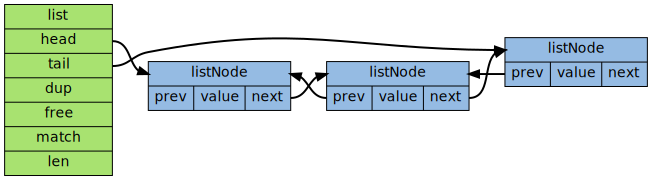
\includegraphics{graphviz-784672591f106642e353f784c9d64cec7a2adb26.pdf}

其中, \code{listNode} 是双端链表的节点:

\begin{Verbatim}[commandchars=\\\{\}]
\PYG{k}{typedef} \PYG{k}{struct} \PYG{n}{listNode} \PYG{p}{\PYGZob{}}

    \PYG{c+c1}{// 前驱节点}
    \PYG{k}{struct} \PYG{n}{listNode} \PYG{o}{*}\PYG{n}{prev}\PYG{p}{;}

    \PYG{c+c1}{// 后继节点}
    \PYG{k}{struct} \PYG{n}{listNode} \PYG{o}{*}\PYG{n}{next}\PYG{p}{;}

    \PYG{c+c1}{// 值}
    \PYG{k+kt}{void} \PYG{o}{*}\PYG{n}{value}\PYG{p}{;}

\PYG{p}{\PYGZcb{}} \PYG{n}{listNode}\PYG{p}{;}
\end{Verbatim}

而 \code{list} 则是双端链表本身:

\begin{Verbatim}[commandchars=\\\{\}]
\PYG{k}{typedef} \PYG{k}{struct} \PYG{n}{list} \PYG{p}{\PYGZob{}}

    \PYG{c+c1}{// 表头指针}
    \PYG{n}{listNode} \PYG{o}{*}\PYG{n}{head}\PYG{p}{;}

    \PYG{c+c1}{// 表尾指针}
    \PYG{n}{listNode} \PYG{o}{*}\PYG{n}{tail}\PYG{p}{;}

    \PYG{c+c1}{// 节点数量}
    \PYG{k+kt}{unsigned} \PYG{k+kt}{long} \PYG{n}{len}\PYG{p}{;}

    \PYG{c+c1}{// 复制函数}
    \PYG{k+kt}{void} \PYG{o}{*}\PYG{p}{(}\PYG{o}{*}\PYG{n}{dup}\PYG{p}{)}\PYG{p}{(}\PYG{k+kt}{void} \PYG{o}{*}\PYG{n}{ptr}\PYG{p}{)}\PYG{p}{;}
    \PYG{c+c1}{// 释放函数}
    \PYG{k+kt}{void} \PYG{p}{(}\PYG{o}{*}\PYG{n}{free}\PYG{p}{)}\PYG{p}{(}\PYG{k+kt}{void} \PYG{o}{*}\PYG{n}{ptr}\PYG{p}{)}\PYG{p}{;}
    \PYG{c+c1}{// 比对函数}
    \PYG{k+kt}{int} \PYG{p}{(}\PYG{o}{*}\PYG{n}{match}\PYG{p}{)}\PYG{p}{(}\PYG{k+kt}{void} \PYG{o}{*}\PYG{n}{ptr}\PYG{p}{,} \PYG{k+kt}{void} \PYG{o}{*}\PYG{n}{key}\PYG{p}{)}\PYG{p}{;}
\PYG{p}{\PYGZcb{}} \PYG{n}{list}\PYG{p}{;}
\end{Verbatim}

注意, \code{listNode} 的 \code{value} 属性的类型是 \code{void *} ,说明这个双端链表对节点所保存的值的类型不做限制。

对于不同类型的值,有时候需要不同的函数来处理这些值,因此, \code{list} 类型保留了三个函数指针 —— \code{dup} 、 \code{free} 和 \code{match} ,分别用于处理值的复制、释放和对比匹配。在对节点的值进行处理时,如果有给定这些函数,那么它们就会被调用。

举个例子:当删除一个 \code{listNode} 时,如果包含这个节点的 \code{list} 的 \code{list-\textgreater{}free} 函数不为空,那么删除函数就会先调用 \code{list-\textgreater{}free(listNode-\textgreater{}value)} 清空节点的值,再执行余下的删除操作(比如说,释放节点)。

另外,从这两个数据结构的定义上,也可以它们的一些行为和性能特征:
\begin{itemize}
\item {} 
\code{listNode} 带有 \code{prev} 和 \code{next} 两个指针,因此,对链表的遍历可以在两个方向上进行:从表头到表尾,或者从表尾到表头。

\item {} 
\code{list} 保存了 \code{head} 和 \code{tail} 两个指针,因此,对链表的表头和表尾进行插入的复杂度都为 $\theta(1)$ —— 这是高效实现 \href{http://redis.readthedocs.org/en/latest/list/lpush.html\#lpush}{\emph{LPUSH}} 、 \href{http://redis.readthedocs.org/en/latest/list/rpop.html\#rpop}{\emph{RPOP}} 、 \href{http://redis.readthedocs.org/en/latest/list/rpoplpush.html\#rpoplpush}{\emph{RPOPLPUSH}} 等命令的关键。

\item {} 
\code{list} 带有保存节点数量的 \code{len} 属性,所以计算链表长度的复杂度仅为 $\theta(1)$ ,这也保证了 \href{http://redis.readthedocs.org/en/latest/list/llen.html\#llen}{\emph{LLEN}} 命令不会成为性能瓶颈。

\end{itemize}

以下是用于操作双端链表的 API ,它们的作用以及算法复杂度:

\begin{tabulary}{\linewidth}{|L|L|L|}
\hline
\textbf{
函数
} & \textbf{
作用
} & \textbf{
算法复杂度
}\\\hline

\code{listCreate}
 & 
创建一个新链表
 & 
$O(1)$
\\\hline

\code{listRelease}
 & 
释放一个链表,以及该链表所包含的节点
 & 
$O(N)$
\\\hline

\code{listDup}
 & 
创建一个给定链表的副本
 & 
$O(N)$
\\\hline

\code{listRotate}
 & 
取出链表的表尾节点,将它插入到表头
 & 
$O(1)$
\\\hline

\code{listAddNodeHead}
 & 
将一个包含给定值的节点添加到链表的表头
 & 
$O(1)$
\\\hline

\code{listAddNodeTail}
 & 
将一个包含给定值的节点添加到链表的表尾
 & 
$O(1)$
\\\hline

\code{listInsertNode}
 & 
将一个包含给定值的节点添加到某个节点的之前或之后
 & 
$O(1)$
\\\hline

\code{listDelNode}
 & 
删除给定节点
 & 
$O(1)$
\\\hline

\code{listSearchKey}
 & 
在链表中查找和给定 key 匹配的节点
 & 
$O(N)$
\\\hline

\code{listIndex}
 & 
给据给定索引,返回列表中相应的节点
 & 
$O(N)$
\\\hline

\code{listLength}
 & 
返回给定链表的节点数量
 & 
$O(1)$
\\\hline

\code{listFirst}
 & 
返回链表的表头节点
 & 
$O(1)$
\\\hline

\code{listLast}
 & 
返回链表的表尾节点
 & 
$O(1)$
\\\hline

\code{listPrevNode}
 & 
返回给定节点的前一个节点
 & 
$O(1)$
\\\hline

\code{listNextNode}
 & 
返回给定节点的后一个节点
 & 
$O(1)$
\\\hline

\code{listNodeValue}
 & 
返回给定节点的值
 & 
$O(1)$
\\\hline
\end{tabulary}



\subsection{迭代器}
\label{internal-datastruct/adlist:id7}
Redis 为双端链表实现了一个\href{http://en.wikipedia.org/wiki/Iterator}{迭代器} ,
这个迭代器可以从两个方向对双端链表进行迭代:
\begin{itemize}
\item {} 
沿着节点的 \code{next} 指针前进,从表头向表尾迭代;

\item {} 
沿着节点的 \code{prev} 指针前进,从表尾向表头迭代;

\end{itemize}

以下是迭代器的数据结构定义:

\begin{Verbatim}[commandchars=\\\{\}]
\PYG{k}{typedef} \PYG{k}{struct} \PYG{n}{listIter} \PYG{p}{\PYGZob{}}

    \PYG{c+c1}{// 下一节点}
    \PYG{n}{listNode} \PYG{o}{*}\PYG{n}{next}\PYG{p}{;}

    \PYG{c+c1}{// 迭代方向}
    \PYG{k+kt}{int} \PYG{n}{direction}\PYG{p}{;}

\PYG{p}{\PYGZcb{}} \PYG{n}{listIter}\PYG{p}{;}
\end{Verbatim}

\code{direction} 记录迭代应该从那里开始:
\begin{itemize}
\item {} 
如果值为 \code{adlist.h/AL\_START\_HEAD} ,那么迭代器执行从表头到表尾的迭代;

\item {} 
如果值为 \code{adlist.h/AL\_START\_TAIL} ,那么迭代器执行从表尾到表头的迭代;

\end{itemize}

以下是迭代器的操作 API ,它们的作用以及算法复杂度:

\begin{tabulary}{\linewidth}{|L|L|L|}
\hline
\textbf{
函数
} & \textbf{
作用
} & \textbf{
算法复杂度
}\\\hline

\code{listGetIterator}
 & 
创建一个列表迭代器
 & 
$O(1)$
\\\hline

\code{listReleaseIterator}
 & 
释放迭代器
 & 
$O(1)$
\\\hline

\code{listRewind}
 & 
将迭代器的指针指向表头
 & 
$O(1)$
\\\hline

\code{listRewindTail}
 & 
将迭代器的指针指向表尾
 & 
$O(1)$
\\\hline

\code{listNext}
 & 
取出迭代器当前指向的节点
 & 
$O(1)$
\\\hline
\end{tabulary}



\subsection{小结}
\label{internal-datastruct/adlist:id9}\begin{itemize}
\item {} 
Redis 实现了自己的双端链表结构。

\item {} 
双端链表主要有两个作用:
\begin{itemize}
\item {} 
作为 Redis 列表类型的底层实现之一;

\item {} 
作为通用数据结构,被其他功能模块所使用;

\end{itemize}

\item {} 
双端链表及其节点的性能特性如下:
\begin{itemize}
\item {} 
节点带有前驱和后继指针,访问前驱节点和后继节点的复杂度为 $O(1)$ ,并且对链表的迭代可以在从表头到表尾和从表尾到表头两个方向进行;

\item {} 
链表带有指向表头和表尾的指针,因此对表头和表尾进行处理的复杂度为 $O(1)$ ;

\item {} 
链表带有记录节点数量的属性,所以可以在 $O(1)$ 复杂度内返回链表的节点数量(长度);

\end{itemize}

\end{itemize}


\section{字典}
\label{internal-datastruct/dict:dict-chapter}\label{internal-datastruct/dict::doc}\label{internal-datastruct/dict:id1}
\href{http://en.wikipedia.org/wiki/Associative\_array}{字典(dictionary),
又名映射(map)或关联数组(associative array),}
它是一种抽象数据结构,
由一集键值对(key-value pairs)组成,
各个键值对的键各不相同,
程序可以将新的键值对添加到字典中,
或者基于键进行查找、更新或删除等操作。

本章先对字典在 Redis 中的应用进行介绍,
接着讲解字典的具体实现方式,
以及这个字典实现要解决的问题,
最后,
以对字典迭代器的介绍作为本章的结束。


\subsection{字典的应用}
\label{internal-datastruct/dict:id2}
字典在 Redis 中的应用广泛,
使用频率可以说和 SDS 以及双端链表不相上下,
基本上各个功能模块都有用到字典的地方。

其中,
字典的主要用途有以下两个:
\begin{enumerate}
\item {} 
实现数据库键空间(key space);

\item {} 
用作 Hash 类型键的其中一种底层实现;

\end{enumerate}

以下两个小节分别介绍这两种用途。


\subsubsection{实现数据库键空间}
\label{internal-datastruct/dict:id3}
Redis 是一个键值对数据库,
数据库中的键值对就由字典保存:
每个数据库都有一个与之相对应的字典,
这个字典被称之为键空间(key space)。

当用户添加一个键值对到数据库时(不论键值对是什么类型),
程序就将该键值对添加到键空间;
当用户从数据库中删除一个键值对时,
程序就会将这个键值对从键空间中删除;
等等。

举个例子,执行 \href{http://redis.readthedocs.org/en/latest/server/flushdb.html\#flushdb}{\emph{FLUSHDB}} 可以清空键空间上的所有键值对数据:

\begin{Verbatim}[commandchars=\\\{\}]
\PYG{n}{redis}\PYG{o}{\PYGZgt{}} \PYG{n}{FLUSHDB}
\PYG{n}{OK}
\end{Verbatim}

执行 \href{http://redis.readthedocs.org/en/latest/server/dbsize.html\#dbsize}{\emph{DBSIZE}} 则返回键空间上现有的键值对:

\begin{Verbatim}[commandchars=\\\{\}]
\PYG{n}{redis}\PYG{o}{\PYGZgt{}} \PYG{n}{DBSIZE}
\PYG{p}{(}\PYG{n}{integer}\PYG{p}{)} \PYG{l+m+mi}{0}
\end{Verbatim}

还可以用 \href{http://redis.readthedocs.org/en/latest/string/set.html\#set}{\emph{SET}} 设置一个字符串键到键空间,
并用 \href{http://redis.readthedocs.org/en/latest/string/get.html\#get}{\emph{GET}} 从键空间中取出该字符串键的值:

\begin{Verbatim}[commandchars=\\\{\}]
\PYG{n}{redis}\PYG{o}{\PYGZgt{}} \PYG{n}{SET} \PYG{n}{number} \PYG{l+m+mi}{10086}
\PYG{n}{OK}

\PYG{n}{redis}\PYG{o}{\PYGZgt{}} \PYG{n}{GET} \PYG{n}{number}
\PYG{l+s}{"}\PYG{l+s}{10086}\PYG{l+s}{"}

\PYG{n}{redis}\PYG{o}{\PYGZgt{}} \PYG{n}{DBSIZE}
\PYG{p}{(}\PYG{n}{integer}\PYG{p}{)} \PYG{l+m+mi}{1}
\end{Verbatim}

后面的《{\hyperref[internal/db:db-chapter]{\emph{数据库}}}》一章会对键空间以及数据库的实现作详细的介绍,
到时我们将看到,
大部分针对数据库的命令,
比如 \href{http://redis.readthedocs.org/en/latest/server/dbsize.html\#dbsize}{\emph{DBSIZE}} 、 \href{http://redis.readthedocs.org/en/latest/server/flushdb.html\#flushdb}{\emph{FLUSHDB}} 、:ref:\emph{RANDOMKEY} ,
等等,
都是构建于对字典的操作之上的;
而那些创建、更新、删除和查找键值对的命令,
也无一例外地需要在键空间上进行操作。


\subsubsection{用作 Hash 类型键的其中一种底层实现}
\label{internal-datastruct/dict:hash}
Redis 的 Hash 类型键使用以下两种数据结构作为底层实现:
\begin{enumerate}
\item {} 
字典;

\item {} 
{\hyperref[compress-datastruct/ziplist:ziplist-chapter]{\emph{压缩列表}}};

\end{enumerate}

因为压缩列表比字典更节省内存,
所以程序在创建新 Hash 键时,
默认使用压缩列表作为底层实现,
当有需要时,
程序才会将底层实现从压缩列表转换到字典。

当用户操作一个 Hash 键时,
键值在底层就可能是一个哈希表:

\begin{Verbatim}[commandchars=\\\{\}]
\PYG{n}{redis}\PYG{o}{\PYGZgt{}} \PYG{n}{HSET} \PYG{n}{book} \PYG{n}{name} \PYG{l+s}{"}\PYG{l+s}{The design and implementation of Redis}\PYG{l+s}{"}
\PYG{p}{(}\PYG{n}{integer}\PYG{p}{)} \PYG{l+m+mi}{1}

\PYG{n}{redis}\PYG{o}{\PYGZgt{}} \PYG{n}{HSET} \PYG{n}{book} \PYG{n}{type} \PYG{l+s}{"}\PYG{l+s}{source code analysis}\PYG{l+s}{"}
\PYG{p}{(}\PYG{n}{integer}\PYG{p}{)} \PYG{l+m+mi}{1}

\PYG{n}{redis}\PYG{o}{\PYGZgt{}} \PYG{n}{HSET} \PYG{n}{book} \PYG{n}{release}\PYG{o}{-}\PYG{n}{date} \PYG{l+s}{"}\PYG{l+s}{2013.3.8}\PYG{l+s}{"}
\PYG{p}{(}\PYG{n}{integer}\PYG{p}{)} \PYG{l+m+mi}{1}

\PYG{n}{redis}\PYG{o}{\PYGZgt{}} \PYG{n}{HGETALL} \PYG{n}{book}
\PYG{l+m+mi}{1}\PYG{p}{)} \PYG{l+s}{"}\PYG{l+s}{name}\PYG{l+s}{"}
\PYG{l+m+mi}{2}\PYG{p}{)} \PYG{l+s}{"}\PYG{l+s}{The design and implementation of Redis}\PYG{l+s}{"}
\PYG{l+m+mi}{3}\PYG{p}{)} \PYG{l+s}{"}\PYG{l+s}{type}\PYG{l+s}{"}
\PYG{l+m+mi}{4}\PYG{p}{)} \PYG{l+s}{"}\PYG{l+s}{source code analysis}\PYG{l+s}{"}
\PYG{l+m+mi}{5}\PYG{p}{)} \PYG{l+s}{"}\PYG{l+s}{release-date}\PYG{l+s}{"}
\PYG{l+m+mi}{6}\PYG{p}{)} \PYG{l+s}{"}\PYG{l+s}{2013.3.8}\PYG{l+s}{"}
\end{Verbatim}

《{\hyperref[datatype/hash:hash-chapter]{\emph{哈希表}}}》章节给出了关于哈希类型键的更多信息,
并介绍了压缩列表和字典之间的转换条件。

介绍完了字典的用途,
现在让我们来看看字典数据结构的定义。


\subsection{字典的实现}
\label{internal-datastruct/dict:id4}
实现字典的方法有很多种:
\begin{itemize}
\item {} 
最简单的就是使用链表或数组, 但是这种方式只适用于元素个数不多的情况下;

\item {} 
要兼顾高效和简单性,可以使用哈希表;

\item {} 
如果追求更为稳定的性能特征, 并且希望高效地实现排序操作的话, 则可以使用更为复杂的平衡树;

\end{itemize}

在众多可能的实现中,
Redis 选择了高效且实现简单的哈希表作为字典的底层实现。

\code{dict.h/dict} 给出了这个字典的定义:

\begin{Verbatim}[commandchars=\\\{\}]
\PYG{c+cm}{/*}
\PYG{c+cm}{ * 字典}
\PYG{c+cm}{ *}
\PYG{c+cm}{ * 每个字典使用两个哈希表,用于实现渐进式 rehash}
\PYG{c+cm}{ */}
\PYG{k}{typedef} \PYG{k}{struct} \PYG{n}{dict} \PYG{p}{\PYGZob{}}

    \PYG{c+c1}{// 特定于类型的处理函数}
    \PYG{n}{dictType} \PYG{o}{*}\PYG{n}{type}\PYG{p}{;}

    \PYG{c+c1}{// 类型处理函数的私有数据}
    \PYG{k+kt}{void} \PYG{o}{*}\PYG{n}{privdata}\PYG{p}{;}

    \PYG{c+c1}{// 哈希表(2个)}
    \PYG{n}{dictht} \PYG{n}{ht}\PYG{p}{[}\PYG{l+m+mi}{2}\PYG{p}{]}\PYG{p}{;}

    \PYG{c+c1}{// 记录 rehash 进度的标志,值为-1 表示 rehash 未进行}
    \PYG{k+kt}{int} \PYG{n}{rehashidx}\PYG{p}{;}

    \PYG{c+c1}{// 当前正在运作的安全迭代器数量}
    \PYG{k+kt}{int} \PYG{n}{iterators}\PYG{p}{;}

\PYG{p}{\PYGZcb{}} \PYG{n}{dict}\PYG{p}{;}
\end{Verbatim}

以下是用于处理 \code{dict} 类型的 API ,
它们的作用及相应的算法复杂度:

\begin{tabulary}{\linewidth}{|L|L|L|}
\hline
\textbf{
操作
} & \textbf{
函数
} & \textbf{
算法复杂度
}\\\hline

创建一个新字典
 & 
\code{dictCreate}
 & 
$O(1)$
\\\hline

添加新键值对到字典
 & 
\code{dictAdd}
 & 
$O(1)$
\\\hline

添加或更新给定键的值
 & 
\code{dictReplace}
 & 
$O(1)$
\\\hline

在字典中查找给定键所在的节点
 & 
\code{dictFind}
 & 
$O(1)$
\\\hline

在字典中查找给定键的值
 & 
\code{dictFetchValue}
 & 
$O(1)$
\\\hline

从字典中随机返回一个节点
 & 
\code{dictGetRandomKey}
 & 
$O(N)$
\\\hline

根据给定键,删除字典中的键值对
 & 
\code{dictDelete}
 & 
$O(1)$
\\\hline

清空并释放字典
 & 
\code{dictRelease}
 & 
$O(N)$
\\\hline

清空并重置(但不释放)字典
 & 
\code{dictEmpty}
 & 
$O(N)$
\\\hline

缩小字典
 & 
\code{dictResize}
 & 
$O(N)$
\\\hline

扩大字典
 & 
\code{dictExpand}
 & 
$O(N)$
\\\hline

对字典进行给定步数的 rehash
 & 
\code{dictRehash}
 & 
$O(N)$
\\\hline

在给定毫秒内,对字典进行rehash
 & 
\code{dictRehashMilliseconds}
 & 
$O(N)$
\\\hline
\end{tabulary}

注意 \code{dict} 类型使用了两个指针分别指向两个哈希表。

其中,
0 号哈希表(\code{ht{[}0{]}})是字典主要使用的哈希表,
而 1 号哈希表(\code{ht{[}1{]}})则只有在程序对 0 号哈希表进行 rehash 时才使用。

接下来两个小节将对哈希表的实现,以及哈希表所使用的哈希算法进行介绍。


\subsubsection{哈希表实现}
\label{internal-datastruct/dict:id5}
字典所使用的哈希表实现由 \code{dict.h/dictht} 类型定义:

\begin{Verbatim}[commandchars=\\\{\}]
\PYG{c+cm}{/*}
\PYG{c+cm}{ * 哈希表}
\PYG{c+cm}{ */}
\PYG{k}{typedef} \PYG{k}{struct} \PYG{n}{dictht} \PYG{p}{\PYGZob{}}

    \PYG{c+c1}{// 哈希表节点指针数组(俗称桶,bucket)}
    \PYG{n}{dictEntry} \PYG{o}{*}\PYG{o}{*}\PYG{n}{table}\PYG{p}{;}

    \PYG{c+c1}{// 指针数组的大小}
    \PYG{k+kt}{unsigned} \PYG{k+kt}{long} \PYG{n}{size}\PYG{p}{;}

    \PYG{c+c1}{// 指针数组的长度掩码,用于计算索引值}
    \PYG{k+kt}{unsigned} \PYG{k+kt}{long} \PYG{n}{sizemask}\PYG{p}{;}

    \PYG{c+c1}{// 哈希表现有的节点数量}
    \PYG{k+kt}{unsigned} \PYG{k+kt}{long} \PYG{n}{used}\PYG{p}{;}

\PYG{p}{\PYGZcb{}} \PYG{n}{dictht}\PYG{p}{;}
\end{Verbatim}

\code{table} 属性是一个数组,
数组的每个元素都是一个指向 \code{dictEntry} 结构的指针。

每个 \code{dictEntry} 都保存着一个键值对,
以及一个指向另一个 \code{dictEntry} 结构的指针:

\begin{Verbatim}[commandchars=\\\{\}]
\PYG{c+cm}{/*}
\PYG{c+cm}{ * 哈希表节点}
\PYG{c+cm}{ */}
\PYG{k}{typedef} \PYG{k}{struct} \PYG{n}{dictEntry} \PYG{p}{\PYGZob{}}

    \PYG{c+c1}{// 键}
    \PYG{k+kt}{void} \PYG{o}{*}\PYG{n}{key}\PYG{p}{;}

    \PYG{c+c1}{// 值}
    \PYG{k}{union} \PYG{p}{\PYGZob{}}
        \PYG{k+kt}{void} \PYG{o}{*}\PYG{n}{val}\PYG{p}{;}
        \PYG{k+kt}{uint64\PYGZus{}t} \PYG{n}{u64}\PYG{p}{;}
        \PYG{k+kt}{int64\PYGZus{}t} \PYG{n}{s64}\PYG{p}{;}
    \PYG{p}{\PYGZcb{}} \PYG{n}{v}\PYG{p}{;}

    \PYG{c+c1}{// 链往后继节点}
    \PYG{k}{struct} \PYG{n}{dictEntry} \PYG{o}{*}\PYG{n}{next}\PYG{p}{;}

\PYG{p}{\PYGZcb{}} \PYG{n}{dictEntry}\PYG{p}{;}
\end{Verbatim}

\code{next} 属性指向另一个 \code{dictEntry} 结构,
多个 \code{dictEntry} 可以通过 \code{next} 指针串连成链表,
从这里可以看出,
\code{dictht} \href{http://en.wikipedia.org/wiki/Hash\_table\#Separate\_chaining}{使用链地址法来处理键碰撞}:
当多个不同的键拥有相同的哈希值时,哈希表用一个链表将这些键连接起来。

下图展示了一个由 \code{dictht} 和数个 \code{dictEntry} 组成的哈希表例子:

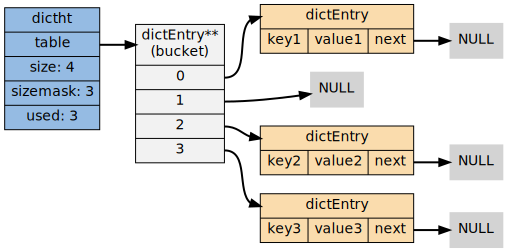
\includegraphics{graphviz-c720caba6b4d02c54fe310c148f0d56316ee80a2.pdf}

如果再加上之前列出的 \code{dict} 类型,那么整个字典结构可以表示如下:

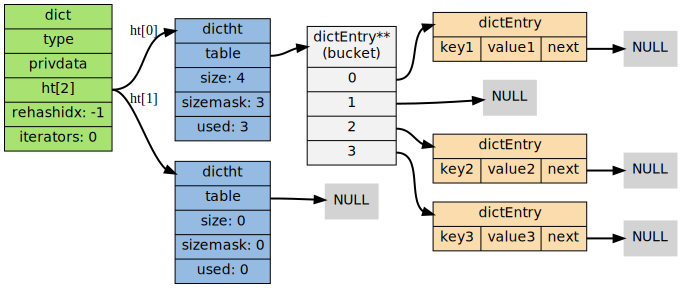
\includegraphics{graphviz-6989792733a041b23cdc0b8f126434590c50a4e4.pdf}

在上图的字典示例中,
字典虽然创建了两个哈希表,
但正在使用的只有 0 号哈希表,
这说明字典未进行 rehash 状态。


\subsubsection{哈希算法}
\label{internal-datastruct/dict:id7}
Redis 目前使用两种不同的哈希算法:
\begin{enumerate}
\item {} 
MurmurHash2 32 bit 算法:这种算法的分布率和速度都非常好, 具体信息请参考 MurmurHash 的主页: \href{http://code.google.com/p/smhasher/}{http://code.google.com/p/smhasher/} 。

\item {} 
基于 djb 算法实现的一个大小写无关散列算法:具体信息请参考 \href{http://www.cse.yorku.ca/~oz/hash.html}{http://www.cse.yorku.ca/\textasciitilde{}oz/hash.html} 。

\end{enumerate}

使用哪种算法取决于具体应用所处理的数据:
\begin{itemize}
\item {} 
命令表以及 Lua 脚本缓存都用到了算法 2 。

\item {} 
算法 1 的应用则更加广泛:数据库、集群、哈希键、阻塞操作等功能都用到了这个算法。

\end{itemize}


\subsection{创建新字典}
\label{internal-datastruct/dict:id8}
\code{dictCreate} 函数创建并返回一个新字典:

\begin{Verbatim}[commandchars=\\\{\}]
\PYG{n}{dict} \PYG{o}{*}\PYG{n}{d} \PYG{o}{=} \PYG{n}{dictCreate}\PYG{p}{(}\PYG{o}{\PYGZam{}}\PYG{n}{hash\PYGZus{}type}\PYG{p}{,} \PYG{n+nb}{NULL}\PYG{p}{)}\PYG{p}{;}
\end{Verbatim}

\code{d} 的值可以用图片表示如下:

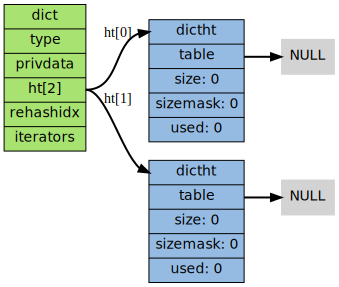
\includegraphics{graphviz-ce90f2a0f396c0ab66b48c0eb83f18fa8f4754f0.pdf}

新创建的两个哈希表都没有为 \code{table} 属性分配任何空间:
\begin{itemize}
\item {} 
\code{ht{[}0{]}-\textgreater{}table} 的空间分配将在第一次往字典添加键值对时进行;

\item {} 
\code{ht{[}1{]}-\textgreater{}table} 的空间分配将在 rehash 开始时进行;

\end{itemize}


\subsection{添加键值对到字典}
\label{internal-datastruct/dict:id9}
根据字典所处的状态,
将一个给定的键值对添加到字典可能会引起一系列复杂的操作:
\begin{itemize}
\item {} 
如果字典为未初始化(也即是字典的 0 号哈希表的 \code{table} 属性为空),那么程序需要对 0 号哈希表进行初始化;

\item {} 
如果在插入时发生了键碰撞,那么程序需要处理碰撞;

\item {} 
如果插入新元素使得字典满足了 rehash 条件,那么需要启动相应的 rehash 程序;

\end{itemize}

当程序处理完以上三种情况之后,新的键值对才会被真正地添加到字典上。

整个添加流程可以用下图表示:

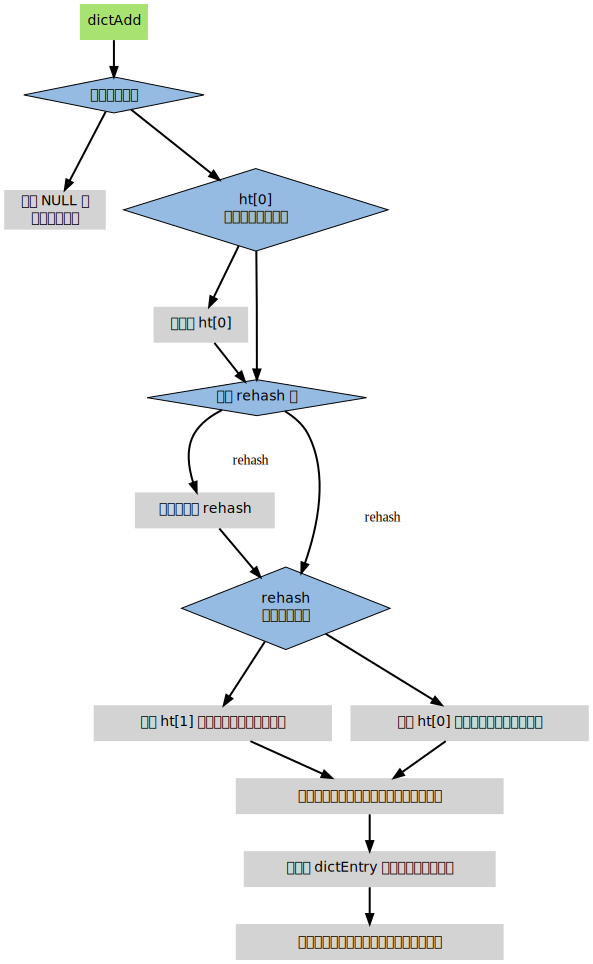
\includegraphics{graphviz-68f4129c529e0c49d38cfe664cad48af4412770a.pdf}

在接下来的三节中,
我们将分别看到添加操作如何在以下三种情况中执行:
\begin{enumerate}
\item {} 
字典为空;

\item {} 
添加新键值对时发生碰撞处理;

\item {} 
添加新键值对时触发了 rehash 操作;

\end{enumerate}


\subsection{添加新元素到空白字典}
\label{internal-datastruct/dict:id10}\label{internal-datastruct/dict:add-when-empty}
当第一次往空字典里添加键值对时,
程序会根据 \code{dict.h/DICT\_HT\_INITIAL\_SIZE} 里指定的大小为
\code{d-\textgreater{}ht{[}0{]}-\textgreater{}table} 分配空间
(在目前的版本中, \code{DICT\_HT\_INITIAL\_SIZE} 的值为 \code{4} )。

以下是字典空白时的样子:

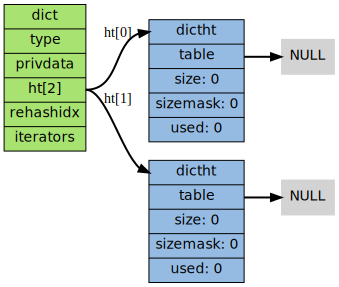
\includegraphics{graphviz-ce90f2a0f396c0ab66b48c0eb83f18fa8f4754f0.pdf}

以下是往空白字典添加了第一个键值对之后的样子:

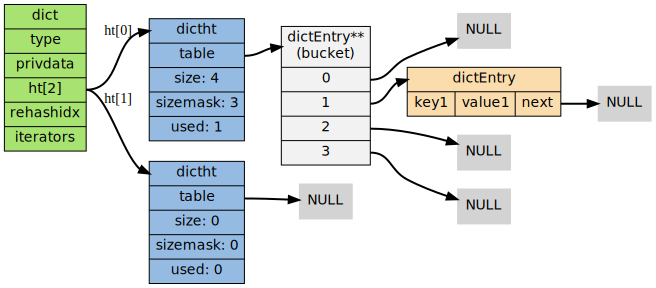
\includegraphics{graphviz-5db645431193228424095abdcf1a3270c9da385e.pdf}


\subsection{添加新键值对时发生碰撞处理}
\label{internal-datastruct/dict:id11}
在哈希表实现中,
当两个不同的键拥有相同的哈希值时,
我们称这两个键发生碰撞(collision),
而哈希表实现必须想办法对碰撞进行处理。

字典哈希表所使用的碰撞解决方法被称之为\href{http://en.wikipedia.org/wiki/Hash\_table\#Separate\_chaining}{链地址法}:
这种方法使用链表将多个哈希值相同的节点串连在一起,
从而解决冲突问题。

假设现在有一个带有三个节点的哈希表,如下图:

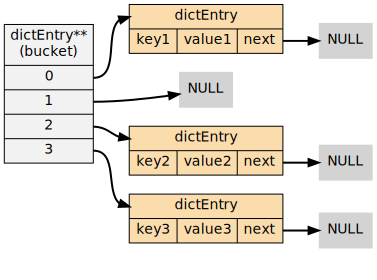
\includegraphics{graphviz-551247f8f670dc6b0eb2dbd6406aee607068249c.pdf}

对于一个新的键值对 \code{key4} 和 \code{value4} ,
如果 \code{key4} 的哈希值和 \code{key1} 的哈希值相同,
那么它们将在哈希表的 \code{0} 号索引上发生碰撞。

通过将 \code{key4-value4} 和 \code{key1-value1} 两个键值对用链表连接起来,
就可以解决碰撞的问题:

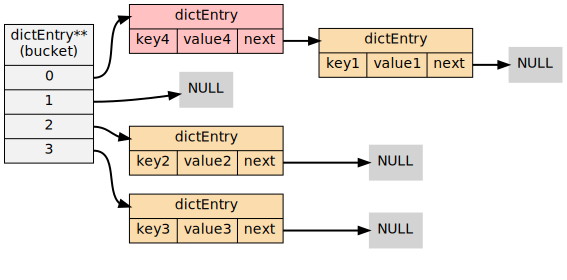
\includegraphics{graphviz-f351812afbaf4b7c29731b38d17dc4a24f902069.pdf}


\subsection{添加新键值对时触发了 rehash 操作}
\label{internal-datastruct/dict:rehash}
对于使用链地址法来解决碰撞问题的哈希表 \code{dictht} 来说,
哈希表的性能依赖于它的大小(\code{size}属性)和它所保存的节点的数量(\code{used}属性)之间的比率:
\begin{itemize}
\item {} 
比率在 1:1 时,哈希表的性能最好;

\item {} 
如果节点数量比哈希表的大小要大很多的话,那么哈希表就会退化成多个链表,哈希表本身的性能优势就不再存在;

\end{itemize}

举个例子,
对于下面这个哈希表,
平均每次失败查找只需要访问 1 个节点(非空节点访问 2 次,空节点访问 1 次):

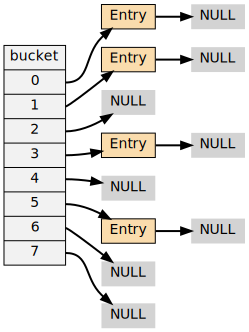
\includegraphics{graphviz-ff857f0c77749cd0213041b561bac0a6348f78e5.pdf}

而对于下面这个哈希表,
平均每次失败查找需要访问 5 个节点:

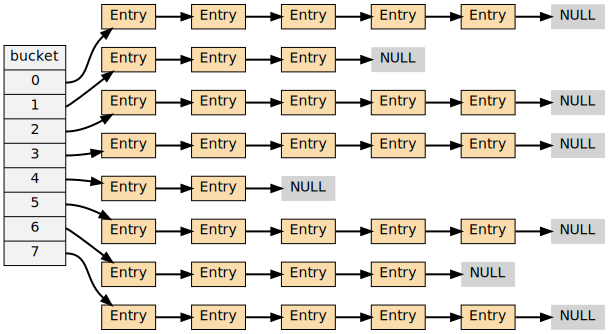
\includegraphics{graphviz-cbec5e98bba611d3021b57f5417b93538328af42.pdf}

为了在字典的键值对不断增多的情况下保持良好的性能,
字典需要对所使用的哈希表(\code{ht{[}0{]}})进行 rehash 操作:
在不修改任何键值对的情况下,对哈希表进行扩容,
尽量将比率维持在 1:1 左右。

\code{dictAdd} 在每次向字典添加新键值对之前, 都会对哈希表 \code{ht{[}0{]}} 进行检查,
对于 \code{ht{[}0{]}} 的 \code{size} 和 \code{used} 属性,
如果它们之间的比率 \code{ratio = used / size} 满足以下任何一个条件的话,rehash 过程就会被激活:
\begin{enumerate}
\item {} 
自然 rehash : \code{ratio \textgreater{}= 1} ,且变量 \code{dict\_can\_resize} 为真。

\item {} 
强制 rehash : \code{ratio} 大于变量 \code{dict\_force\_resize\_ratio} (目前版本中, \code{dict\_force\_resize\_ratio} 的值为 \code{5} )。

\end{enumerate}

\begin{notice}{note}{Note:}
什么时候 \code{dict\_can\_resize} 会为假?

在前面介绍字典的应用时也说到过,
一个数据库就是一个字典,
数据库里的哈希类型键也是一个字典,
当 Redis 使用子进程对数据库执行后台持久化任务时(比如执行 \code{BGSAVE} 或 \code{BGREWRITEAOF} 时),
为了最大化地利用系统的 \href{http://en.wikipedia.org/wiki/Copy-on-write}{copy on write} 机制,
程序会暂时将 \code{dict\_can\_resize} 设为假,
避免执行自然 rehash ,
从而减少程序对内存的触碰(touch)。

当持久化任务完成之后,
\code{dict\_can\_resize} 会重新被设为真。

另一方面,
当字典满足了强制 rehash 的条件时,
即使 \code{dict\_can\_resize} 不为真(有 \code{BGSAVE} 或 \code{BGREWRITEAOF} 正在执行),
这个字典一样会被 rehash 。
\end{notice}


\subsection{Rehash 执行过程}
\label{internal-datastruct/dict:id13}
字典的 rehash 操作实际上就是执行以下任务:
\begin{enumerate}
\item {} 
创建一个比 \code{ht{[}0{]}-\textgreater{}table} 更大的 \code{ht{[}1{]}-\textgreater{}table} ;

\item {} 
将 \code{ht{[}0{]}-\textgreater{}table} 中的所有键值对迁移到 \code{ht{[}1{]}-\textgreater{}table} ;

\item {} 
将原有 \code{ht{[}0{]}} 的数据清空,并将 \code{ht{[}1{]}} 替换为新的 \code{ht{[}0{]}} ;

\end{enumerate}

经过以上步骤之后,
程序就在不改变原有键值对数据的基础上,
增大了哈希表的大小。

作为例子,
以下四个小节展示了一次对哈希表进行 rehash 的完整过程。


\subsubsection{1. 开始 rehash}
\label{internal-datastruct/dict:id14}
这个阶段有两个事情要做:
\begin{enumerate}
\item {} 
设置字典的 \code{rehashidx} 为 \code{0} ,标识着 rehash 的开始;

\item {} 
为 \code{ht{[}1{]}-\textgreater{}table} 分配空间,大小至少为 \code{ht{[}0{]}-\textgreater{}used} 的两倍;

\end{enumerate}

这时的字典是这个样子:

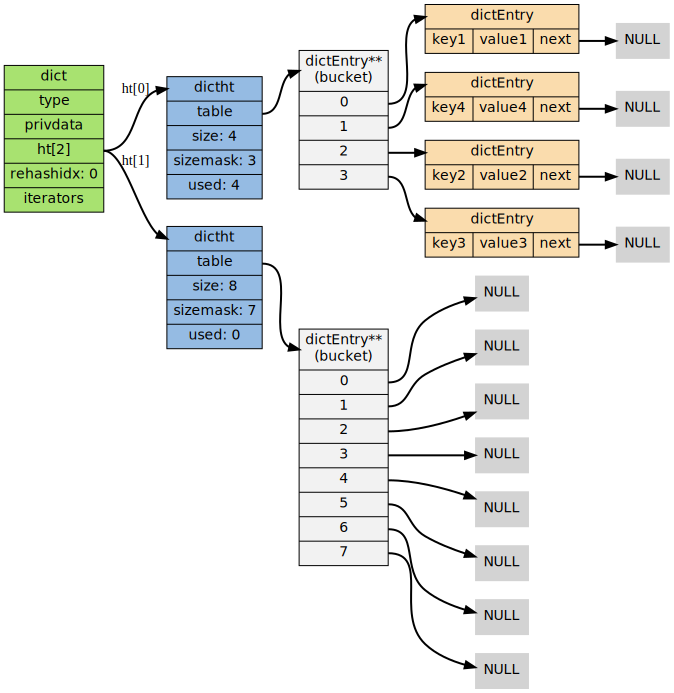
\includegraphics{graphviz-8af45a72833893e88a305ccd461561b9b00a8816.pdf}


\subsubsection{2. Rehash 进行中}
\label{internal-datastruct/dict:id15}
在这个阶段, \code{ht{[}0{]}-\textgreater{}table} 的节点会被逐渐迁移到 \code{ht{[}1{]}-\textgreater{}table} ,
因为 rehash 是分多次进行的(细节在下一节解释),
字典的 \code{rehashidx} 变量会记录 rehash 进行到 \code{ht{[}0{]}} 的哪个索引位置上。

以下是 \code{rehashidx} 值为 \code{2} 时,字典的样子:

\includegraphics{graphviz-8c861670330ef855a2e053e280506d6744e1e5d4.pdf}

注意除了节点的移动外,
字典的 \code{rehashidx} 、 \code{ht{[}0{]}-\textgreater{}used} 和 \code{ht{[}1{]}-\textgreater{}used} 三个属性也产生了变化。


\subsubsection{3. 节点迁移完毕}
\label{internal-datastruct/dict:id16}
到了这个阶段,所有的节点都已经从 \code{ht{[}0{]}} 迁移到 \code{ht{[}1{]}} 了:

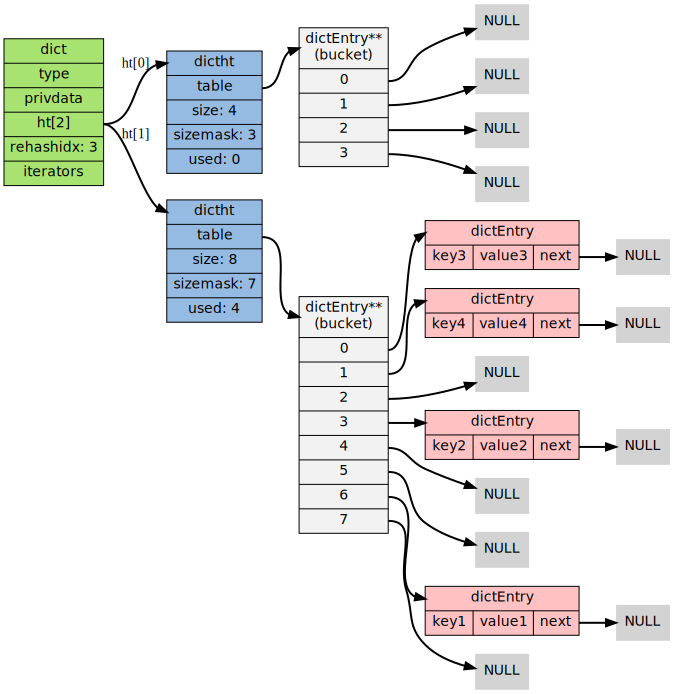
\includegraphics{graphviz-15aedc410b921c8a0fd3183c5141b7d1f1ed6eed.pdf}


\subsubsection{4. Rehash 完毕}
\label{internal-datastruct/dict:id17}
在 rehash 的最后阶段,程序会执行以下工作:
\begin{enumerate}
\item {} 
释放 \code{ht{[}0{]}} 的空间;

\item {} 
用 \code{ht{[}1{]}} 来代替 \code{ht{[}0{]}} ,使原来的 \code{ht{[}1{]}} 成为新的 \code{ht{[}0{]}} ;

\item {} 
创建一个新的空哈希表,并将它设置为 \code{ht{[}1{]}} ;

\item {} 
将字典的 \code{rehashidx} 属性设置为 \code{-1} ,标识 rehash 已停止;

\end{enumerate}

以下是字典 rehash 完毕之后的样子:

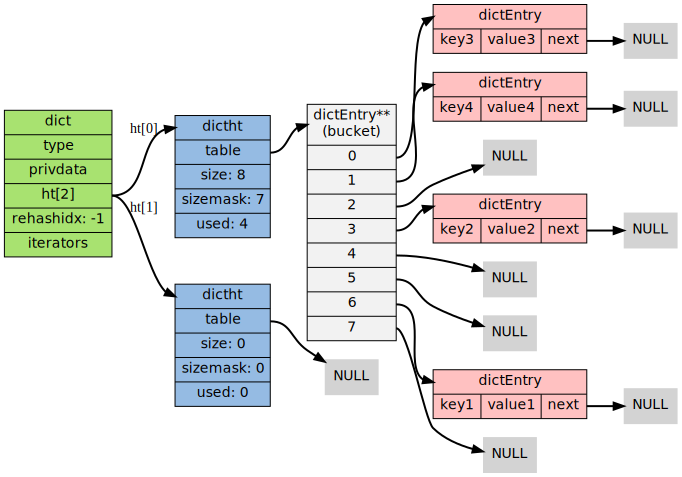
\includegraphics{graphviz-6d5b0f4115d30fac37af21f3834b5554d8824923.pdf}

对比字典 rehash 之前和 rehash 之后,
新的 \code{ht{[}0{]}} 空间更大,
并且字典原有的键值对也没有被修改或者删除。


\subsection{渐进式 rehash}
\label{internal-datastruct/dict:id18}
在上一节,我们了解了字典的 rehash 过程,
需要特别指出的是, rehash 程序并不是在激活之后就马上执行直到完成的,
而是分多次、渐进式地完成的。

假设这样一个场景:在一个有很多键值对的字典里,
某个用户在添加新键值对时触发了 rehash 过程,
如果这个 rehash 过程必须将所有键值对迁移完毕之后才将结果返回给用户,
这样的处理方式将是非常不友好的。

另一方面,
要求服务器必须阻塞直到 rehash 完成,
这对于 Redis 服务器本身也是不能接受的。

为了解决这个问题,
Redis 使用了渐进式(incremental)的 rehash 方式:
通过将 rehash 分散到多个步骤中进行,
从而避免了集中式的计算。

渐进式 rehash 主要由 \code{\_dictRehashStep} 和 \code{dictRehashMilliseconds} 两个函数进行:
\begin{itemize}
\item {} 
\code{\_dictRehashStep} 用于对数据库字典、以及哈希键的字典进行被动 rehash ;

\item {} 
\code{dictRehashMilliseconds} 则由 Redis 服务器常规任务程序(server cron job)执行,用于对数据库字典进行主动 rehash ;

\end{itemize}


\subsubsection{\_dictRehashStep}
\label{internal-datastruct/dict:dictrehashstep}
每次执行 \code{\_dictRehashStep} ,
\code{ht{[}0{]}-\textgreater{}table} 哈希表第一个不为空的索引上的所有节点就会全部迁移到 \code{ht{[}1{]}-\textgreater{}table} 。

在 rehash 开始进行之后(\code{d-\textgreater{}rehashidx} 不为 \code{-1}),
每次执行一次添加、查找、删除操作,
\code{\_dictRehashStep} 都会被执行一次:

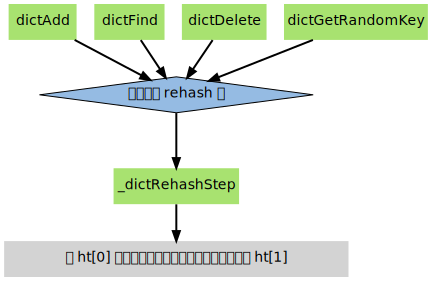
\includegraphics{graphviz-121adbc9859ad43720ccb8d4d91bf28062af3256.pdf}

因为字典会保持哈希表大小和节点数的比率在一个很小的范围内,
所以每个索引上的节点数量不会很多(从目前版本的 rehash 条件来看,平均只有一个,最多通常也不会超过五个),
所以在执行操作的同时,对单个索引上的节点进行迁移,
几乎不会对响应时间造成影响。


\subsubsection{dictRehashMilliseconds}
\label{internal-datastruct/dict:dictrehashmilliseconds}
\code{dictRehashMilliseconds} 可以在指定的毫秒数内,
对字典进行 rehash 。

当 Redis 的服务器常规任务执行时,
\code{dictRehashMilliseconds} 会被执行,
在规定的时间内,
尽可能地对数据库字典中那些需要 rehash 的字典进行 rehash ,
从而加速数据库字典的 rehash 进程(progress)。


\subsubsection{其他措施}
\label{internal-datastruct/dict:id19}
在哈希表进行 rehash 时,
字典还会采取一些特别的措施,
确保 rehash 顺利、正确地进行:
\begin{itemize}
\item {} 
因为在 rehash 时,字典会同时使用两个哈希表,所以在这期间的所有查找、删除等操作,除了在 \code{ht{[}0{]}} 上进行,还需要在 \code{ht{[}1{]}} 上进行。

\item {} 
在执行添加操作时,新的节点会直接添加到 \code{ht{[}1{]}} 而不是 \code{ht{[}0{]}} ,这样保证 \code{ht{[}0{]}} 的节点数量在整个 rehash 过程中都只减不增。

\end{itemize}


\subsection{字典的收缩}
\label{internal-datastruct/dict:id20}
上面关于 rehash 的章节描述了通过 rehash 对字典进行扩展(expand)的情况,
如果哈希表的可用节点数比已用节点数大很多的话,
那么也可以通过对哈希表进行 rehash 来收缩(shrink)字典。

收缩 rehash 和上面展示的扩展 rehash 的操作几乎一样,它执行以下步骤:
\begin{enumerate}
\item {} 
创建一个比 \code{ht{[}0{]}-\textgreater{}table} 小的 \code{ht{[}1{]}-\textgreater{}table} ;

\item {} 
将 \code{ht{[}0{]}-\textgreater{}table} 中的所有键值对迁移到 \code{ht{[}1{]}-\textgreater{}table} ;

\item {} 
将原有 \code{ht{[}0{]}} 的数据清空,并将 \code{ht{[}1{]}} 替换为新的 \code{ht{[}0{]}} ;

\end{enumerate}

扩展 rehash 和收缩 rehash 执行完全相同的过程,
一个 rehash 是扩展还是收缩字典,
关键在于新分配的 \code{ht{[}1{]}-\textgreater{}table} 的大小:
\begin{itemize}
\item {} 
如果 rehash 是扩展操作,那么 \code{ht{[}1{]}-\textgreater{}table} 比 \code{ht{[}0{]}-\textgreater{}table} 要大;

\item {} 
如果 rehash 是收缩操作,那么 \code{ht{[}1{]}-\textgreater{}table} 比 \code{ht{[}0{]}-\textgreater{}table} 要小;

\end{itemize}

字典的收缩规则由 \code{redis.c/htNeedsResize} 函数定义:

\begin{Verbatim}[commandchars=\\\{\}]
\PYG{c+cm}{/*}
\PYG{c+cm}{ * 检查字典的使用率是否低于系统允许的最小比率}
\PYG{c+cm}{ *}
\PYG{c+cm}{ * 是的话返回 1 ,否则返回 0 。}
\PYG{c+cm}{ */}
\PYG{k+kt}{int} \PYG{n+nf}{htNeedsResize}\PYG{p}{(}\PYG{n}{dict} \PYG{o}{*}\PYG{n}{dict}\PYG{p}{)} \PYG{p}{\PYGZob{}}
    \PYG{k+kt}{long} \PYG{k+kt}{long} \PYG{n}{size}\PYG{p}{,} \PYG{n}{used}\PYG{p}{;}

    \PYG{c+c1}{// 哈希表已用节点数量}
    \PYG{n}{size} \PYG{o}{=} \PYG{n}{dictSlots}\PYG{p}{(}\PYG{n}{dict}\PYG{p}{)}\PYG{p}{;}

    \PYG{c+c1}{// 哈希表大小}
    \PYG{n}{used} \PYG{o}{=} \PYG{n}{dictSize}\PYG{p}{(}\PYG{n}{dict}\PYG{p}{)}\PYG{p}{;}

    \PYG{c+c1}{// 当哈希表的大小大于 DICT\PYGZus{}HT\PYGZus{}INITIAL\PYGZus{}SIZE}
    \PYG{c+c1}{// 并且字典的填充率低于 REDIS\PYGZus{}HT\PYGZus{}MINFILL 时}
    \PYG{c+c1}{// 返回 1}
    \PYG{k}{return} \PYG{p}{(}\PYG{n}{size} \PYG{o}{\PYGZam{}}\PYG{o}{\PYGZam{}} \PYG{n}{used} \PYG{o}{\PYGZam{}}\PYG{o}{\PYGZam{}} \PYG{n}{size} \PYG{o}{\PYGZgt{}} \PYG{n}{DICT\PYGZus{}HT\PYGZus{}INITIAL\PYGZus{}SIZE} \PYG{o}{\PYGZam{}}\PYG{o}{\PYGZam{}}
            \PYG{p}{(}\PYG{n}{used}\PYG{o}{*}\PYG{l+m+mi}{100}\PYG{o}{/}\PYG{n}{size} \PYG{o}{\PYGZlt{}} \PYG{n}{REDIS\PYGZus{}HT\PYGZus{}MINFILL}\PYG{p}{)}\PYG{p}{)}\PYG{p}{;}
\PYG{p}{\PYGZcb{}}
\end{Verbatim}

在默认情况下,
\code{REDIS\_HT\_MINFILL} 的值为 \code{10} ,
也即是说,
当字典的填充率低于 10\% 时,
程序就可以对这个字典进行收缩操作了。

字典收缩和字典扩展的一个区别是:
\begin{itemize}
\item {} 
字典的扩展操作是自动触发的(不管是自动扩展还是强制扩展);

\item {} 
而字典的收缩操作则是由程序手动执行。

\end{itemize}

因此,
使用字典的程序可以决定何时对字典进行收缩:
\begin{itemize}
\item {} 
当字典用于实现哈希键的时候,
每次从字典中删除一个键值对,
程序就会执行一次 \code{htNeedsResize} 函数,
如果字典达到了收缩的标准,
程序将立即对字典进行收缩;

\item {} 
当字典用于实现数据库键空间(key space)的时候,
收缩的时机由 \code{redis.c/tryResizeHashTables} 函数决定,
具体信息请参考《{\hyperref[internal/db:db-chapter]{\emph{数据库}}}》一章的《{\hyperref[internal/db:db-expand-and-shrink]{\emph{数据库空间的收缩和扩展}}}》小节;

\end{itemize}




\subsection{字典其他操作}
\label{internal-datastruct/dict:id21}
除了添加操作和伸展/收缩操作之外,
字典还定义了其他一些操作,
比如常见的查找、删除和更新。

因为链地址法哈希表实现的相关信息可以从任何一本数据结构或算法书上找到,
这里不再对字典的其他操作进行介绍,
不过前面对创建字典、添加键值对、收缩和扩展 rehash 的讨论已经涵盖了字典模块的核心内容。


\subsection{字典的迭代}
\label{internal-datastruct/dict:id22}
字典带有自己的\href{http://en.wikipedia.org/wiki/Iterator}{迭代器}实现 ——
对字典进行迭代实际上就是对字典所使用的哈希表进行迭代:
\begin{itemize}
\item {} 
迭代器首先迭代字典的第一个哈希表, 然后,如果 rehash 正在进行的话, 就继续对第二个哈希表进行迭代。

\item {} 
当迭代哈希表时, 找到第一个不为空的索引, 然后迭代这个索引上的所有节点。

\item {} 
当这个索引迭代完了, 继续查找下一个不为空的索引, 如此循环, 一直到整个哈希表都迭代完为止。

\end{itemize}

整个迭代过程可以用伪代码表示如下:

\begin{Verbatim}[commandchars=\\\{\}]
\PYG{k}{def} \PYG{n+nf}{iter\PYGZus{}dict}\PYG{p}{(}\PYG{n+nb}{dict}\PYG{p}{)}\PYG{p}{:}

    \PYG{c}{\PYGZsh{} 迭代 0 号哈希表}
    \PYG{n}{iter\PYGZus{}table}\PYG{p}{(}\PYG{n}{ht}\PYG{p}{[}\PYG{l+m+mi}{0}\PYG{p}{]}\PYG{o}{-}\PYG{o}{\PYGZgt{}}\PYG{n}{table}\PYG{p}{)}

    \PYG{c}{\PYGZsh{} 如果正在执行 rehash ,那么也迭代 1 号哈希表}
    \PYG{k}{if} \PYG{n+nb}{dict}\PYG{o}{.}\PYG{n}{is\PYGZus{}rehashing}\PYG{p}{(}\PYG{p}{)}\PYG{p}{:} \PYG{n}{iter\PYGZus{}table}\PYG{p}{(}\PYG{n}{ht}\PYG{p}{[}\PYG{l+m+mi}{1}\PYG{p}{]}\PYG{o}{-}\PYG{o}{\PYGZgt{}}\PYG{n}{table}\PYG{p}{)}


\PYG{k}{def} \PYG{n+nf}{iter\PYGZus{}table}\PYG{p}{(}\PYG{n}{table}\PYG{p}{)}\PYG{p}{:}

    \PYG{c}{\PYGZsh{} 遍历哈希表上的所有索引}
    \PYG{k}{for} \PYG{n}{index} \PYG{o+ow}{in} \PYG{n}{table}\PYG{p}{:}

        \PYG{c}{\PYGZsh{} 跳过空索引}
        \PYG{k}{if} \PYG{n}{table}\PYG{p}{[}\PYG{n}{index}\PYG{p}{]}\PYG{o}{.}\PYG{n}{empty}\PYG{p}{(}\PYG{p}{)}\PYG{p}{:}
            \PYG{k}{continue}

        \PYG{c}{\PYGZsh{} 遍历索引上的所有节点}
        \PYG{k}{for} \PYG{n}{node} \PYG{o+ow}{in} \PYG{n}{table}\PYG{p}{[}\PYG{n}{index}\PYG{p}{]}\PYG{p}{:}

            \PYG{c}{\PYGZsh{} 处理节点}
            \PYG{n}{do\PYGZus{}something\PYGZus{}with}\PYG{p}{(}\PYG{n}{node}\PYG{p}{)}
\end{Verbatim}

字典的迭代器有两种:
\begin{itemize}
\item {} 
安全迭代器:在迭代进行过程中,可以对字典进行修改。

\item {} 
不安全迭代器: 在迭代进行过程中,不对字典进行修改。

\end{itemize}

以下是迭代器的数据结构定义:

\begin{Verbatim}[commandchars=\\\{\}]
\PYG{c+cm}{/*}
\PYG{c+cm}{ * 字典迭代器}
\PYG{c+cm}{ */}
\PYG{k}{typedef} \PYG{k}{struct} \PYG{n}{dictIterator} \PYG{p}{\PYGZob{}}

    \PYG{n}{dict} \PYG{o}{*}\PYG{n}{d}\PYG{p}{;}                \PYG{c+c1}{// 正在迭代的字典}

    \PYG{k+kt}{int} \PYG{n}{table}\PYG{p}{,}              \PYG{c+c1}{// 正在迭代的哈希表的号码(0 或者 1)}
        \PYG{n}{index}\PYG{p}{,}              \PYG{c+c1}{// 正在迭代的哈希表数组的索引}
        \PYG{n}{safe}\PYG{p}{;}               \PYG{c+c1}{// 是否安全?}

    \PYG{n}{dictEntry} \PYG{o}{*}\PYG{n}{entry}\PYG{p}{,}       \PYG{c+c1}{// 当前哈希节点}
              \PYG{o}{*}\PYG{n}{nextEntry}\PYG{p}{;}   \PYG{c+c1}{// 当前哈希节点的后继节点}

\PYG{p}{\PYGZcb{}} \PYG{n}{dictIterator}\PYG{p}{;}
\end{Verbatim}

以下函数是这个迭代器的 API ,它们的作用及相关算法复杂度:

\begin{tabulary}{\linewidth}{|L|p{8.5cm}|L|}
\hline
\textbf{
函数
} & \textbf{
作用
} & \textbf{
算法复杂度
}\\\hline

\code{dictGetIterator}
 & 
创建一个不安全迭代器。
 & 
$O(1)$
\\\hline

\code{dictGetSafeIterator}
 & 
创建一个安全迭代器。
 & 
$O(1)$
\\\hline

\code{dictNext}
 & 
返回迭代器指向的当前节点,如果迭代完毕,返回 \code{NULL} 。
 & 
$O(1)$
\\\hline

\code{dictReleaseIterator}
 & 
释放迭代器。
 & 
$O(1)$
\\\hline
\end{tabulary}



\subsection{小结}
\label{internal-datastruct/dict:id24}\begin{itemize}
\item {} 
字典由键值对构成的抽象数据结构。

\item {} 
Redis 中的数据库和哈希键都基于字典来实现。

\item {} 
Redis 字典的底层实现为哈希表,每个字典使用两个哈希表,一般情况下只使用 0 号哈希表,只有在 rehash 进行时,才会同时使用 0 号和 1 号哈希表。

\item {} 
哈希表使用链地址法来解决键冲突的问题。

\item {} 
Rehash 可以用于扩展或收缩哈希表。

\item {} 
对哈希表的 rehash 是分多次、渐进式地进行的。

\end{itemize}


\section{跳跃表}
\label{internal-datastruct/skiplist::doc}\label{internal-datastruct/skiplist:id1}
跳跃表(\href{http://en.wikipedia.org/wiki/Skip\_list}{skiplist})是一种随机化的数据,
由 William Pugh 在论文《Skip lists: a probabilistic alternative to balanced trees》中提出,
这种数据结构以有序的方式在层次化的链表中保存元素,
它的效率可以和平衡树媲美 ——
查找、删除、添加等操作都可以在对数期望时间下完成,
并且比起平衡树来说,
跳跃表的实现要简单直观得多。

以下是一个典型的跳跃表例子(图片来自\href{http://en.wikipedia.org/wiki/File:Skip\_list.svg}{维基百科}):

\scalebox{0.800000}{\includegraphics{skiplist.png}}

从图中可以看到,
跳跃表主要由以下部分构成:
\begin{itemize}
\item {} 
表头(head):负责维护跳跃表的节点指针。

\item {} 
跳跃表节点:保存着元素值,以及多个层。

\item {} 
层:保存着指向其他元素的指针。高层的指针越过的元素数量大于等于低层的指针,为了提高查找的效率,程序总是从高层先开始访问,然后随着元素值范围的缩小,慢慢降低层次。

\item {} 
表尾:全部由 \code{NULL} 组成,表示跳跃表的末尾。

\end{itemize}

因为跳跃表的定义可以在任何一本算法或数据结构的书中找到,
所以本章不介绍跳跃表的具体实现方式或者具体的算法,
而只介绍跳跃表在 Redis 的应用、核心数据结构和 API 。


\subsection{跳跃表的实现}
\label{internal-datastruct/skiplist:id3}
为了适应自身的功能需要,
Redis 基于 William Pugh 论文中描述的跳跃表进行了以下修改:
\begin{enumerate}
\item {} 
允许重复的 \code{score} 值:多个不同的 \code{member} 的 \code{score} 值可以相同。

\item {} 
进行对比操作时,不仅要检查 \code{score} 值,还要检查 \code{member} :当 \code{score} 值可以重复时,单靠 \code{score} 值无法判断一个元素的身份,所以需要连 \code{member} 域都一并检查才行。

\item {} 
每个节点都带有一个高度为 1 层的后退指针,用于从表尾方向向表头方向迭代:当执行 \href{http://redis.readthedocs.org/en/latest/sorted\_set/zrevrange.html\#zrevrange}{\emph{ZREVRANGE}} 或 \href{http://redis.readthedocs.org/en/latest/sorted\_set/zrevrangebyscore.html\#zrevrangebyscore}{\emph{ZREVRANGEBYSCORE}} 这类以逆序处理有序集的命令时,就会用到这个属性。

\end{enumerate}

这个修改版的跳跃表由 \code{redis.h/zskiplist} 结构定义:

\begin{Verbatim}[commandchars=\\\{\}]
\PYG{k}{typedef} \PYG{k}{struct} \PYG{n}{zskiplist} \PYG{p}{\PYGZob{}}

    \PYG{c+c1}{// 头节点,尾节点}
    \PYG{k}{struct} \PYG{n}{zskiplistNode} \PYG{o}{*}\PYG{n}{header}\PYG{p}{,} \PYG{o}{*}\PYG{n}{tail}\PYG{p}{;}

    \PYG{c+c1}{// 节点数量}
    \PYG{k+kt}{unsigned} \PYG{k+kt}{long} \PYG{n}{length}\PYG{p}{;}

    \PYG{c+c1}{// 目前表内节点的最大层数}
    \PYG{k+kt}{int} \PYG{n}{level}\PYG{p}{;}

\PYG{p}{\PYGZcb{}} \PYG{n}{zskiplist}\PYG{p}{;}
\end{Verbatim}

跳跃表的节点由 \code{redis.h/zskiplistNode} 定义:

\begin{Verbatim}[commandchars=\\\{\}]
\PYG{k}{typedef} \PYG{k}{struct} \PYG{n}{zskiplistNode} \PYG{p}{\PYGZob{}}

    \PYG{c+c1}{// member 对象}
    \PYG{n}{robj} \PYG{o}{*}\PYG{n}{obj}\PYG{p}{;}

    \PYG{c+c1}{// 分值}
    \PYG{k+kt}{double} \PYG{n}{score}\PYG{p}{;}

    \PYG{c+c1}{// 后退指针}
    \PYG{k}{struct} \PYG{n}{zskiplistNode} \PYG{o}{*}\PYG{n}{backward}\PYG{p}{;}

    \PYG{c+c1}{// 层}
    \PYG{k}{struct} \PYG{n}{zskiplistLevel} \PYG{p}{\PYGZob{}}

        \PYG{c+c1}{// 前进指针}
        \PYG{k}{struct} \PYG{n}{zskiplistNode} \PYG{o}{*}\PYG{n}{forward}\PYG{p}{;}

        \PYG{c+c1}{// 这个层跨越的节点数量}
        \PYG{k+kt}{unsigned} \PYG{k+kt}{int} \PYG{n}{span}\PYG{p}{;}

    \PYG{p}{\PYGZcb{}} \PYG{n}{level}\PYG{p}{[}\PYG{p}{]}\PYG{p}{;}

\PYG{p}{\PYGZcb{}} \PYG{n}{zskiplistNode}\PYG{p}{;}
\end{Verbatim}

以下是操作这两个数据结构的 API ,它们的作用以及相应的算法复杂度:

\begin{tabulary}{\linewidth}{|p{4.3cm}|p{5.8cm}|L|}
\hline
\textbf{
函数
} & \textbf{
作用
} & \textbf{
复杂度
}\\\hline

\code{zslCreateNode}
 & 
创建并返回一个新的跳跃表节点
 & 
最坏 $O(1)$
\\\hline

\code{zslFreeNode}
 & 
释放给定的跳跃表节点
 & 
最坏 $O(1)$
\\\hline

\code{zslCreate}
 & 
创建并初始化一个新的跳跃表
 & 
最坏 $O(N)$
\\\hline

\code{zslFree}
 & 
释放给定的跳跃表
 & 
最坏 $O(N)$
\\\hline

\code{zslInsert}
 & 
将一个包含给定 \code{score} 和 \code{member} 的新节点添加到跳跃表中
 & 
最坏 $O(N)$ 平均 $O(\log N)$
\\\hline

\code{zslDeleteNode}
 & 
删除给定的跳跃表节点
 & 
最坏 $O(N)$
\\\hline

\code{zslDelete}
 & 
删除匹配给定 \code{member} 和 \code{score} 的元素
 & 
最坏 $O(N)$ 平均 $O(\log N)$
\\\hline

\code{zslFirstInRange}
 & 
找到跳跃表中第一个符合给定范围的元素
 & 
最坏 $O(N)$ 平均 $O(\log N)$
\\\hline

\code{zslLastInRange}
 & 
找到跳跃表中最后一个符合给定范围的元素
 & 
最坏 $O(N)$ 平均 $O(\log N)$
\\\hline

\code{zslDeleteRangeByScore}
 & 
删除 \code{score} 值在给定范围内的所有节点
 & 
最坏 $O(N^2)$
\\\hline

\code{zslDeleteRangeByRank}
 & 
删除给定排序范围内的所有节点
 & 
最坏 $O(N^2)$
\\\hline

\code{zslGetRank}
 & 
返回目标元素在有序集中的排位
 & 
最坏 $O(N)$ 平均 $O(\log N)$
\\\hline

\code{zslGetElementByRank}
 & 
根据给定排位,返回该排位上的元素节点
 & 
最坏 $O(N)$ 平均 $O(\log N)$
\\\hline
\end{tabulary}



\subsection{跳跃表的应用}
\label{internal-datastruct/skiplist:id4}
和字典、链表或者字符串这几种在 Redis 中大量使用的数据结构不同,
跳跃表在 Redis 的唯一作用,
就是实现有序集数据类型。

跳跃表将指向有序集的 \code{score} 值和 \code{member} 域的指针作为元素,
并以 \code{score} 值为索引,
对有序集元素进行排序。

举个例子,
以下代码就创建了一个带有 3 个元素的有序集:

\begin{Verbatim}[commandchars=\\\{\}]
\PYG{n}{redis}\PYG{o}{\PYGZgt{}} \PYG{n}{ZADD} \PYG{n}{s} \PYG{l+m+mi}{6} \PYG{n}{x} \PYG{l+m+mi}{10} \PYG{n}{y} \PYG{l+m+mi}{15} \PYG{n}{z}
\PYG{p}{(}\PYG{n}{integer}\PYG{p}{)} \PYG{l+m+mi}{3}

\PYG{n}{redis}\PYG{o}{\PYGZgt{}} \PYG{n}{ZRANGE} \PYG{n}{s} \PYG{l+m+mi}{0} \PYG{o}{-}\PYG{l+m+mi}{1} \PYG{n}{WITHSCORES}
\PYG{l+m+mi}{1}\PYG{p}{)} \PYG{l+s}{"}\PYG{l+s}{x}\PYG{l+s}{"}
\PYG{l+m+mi}{2}\PYG{p}{)} \PYG{l+s}{"}\PYG{l+s}{6}\PYG{l+s}{"}
\PYG{l+m+mi}{3}\PYG{p}{)} \PYG{l+s}{"}\PYG{l+s}{y}\PYG{l+s}{"}
\PYG{l+m+mi}{4}\PYG{p}{)} \PYG{l+s}{"}\PYG{l+s}{10}\PYG{l+s}{"}
\PYG{l+m+mi}{5}\PYG{p}{)} \PYG{l+s}{"}\PYG{l+s}{z}\PYG{l+s}{"}
\PYG{l+m+mi}{6}\PYG{p}{)} \PYG{l+s}{"}\PYG{l+s}{15}\PYG{l+s}{"}
\end{Verbatim}

在底层实现中,
Redis 为 \code{x} 、 \code{y} 和 \code{z} 三个 \code{member} 分别创建了三个字符串,
并为 \code{6} 、 \code{10} 和 \code{15} 分别创建三个 \code{double} 类型的值,
然后用一个跳跃表将这些指针有序地保存起来,
形成这样一个跳跃表:

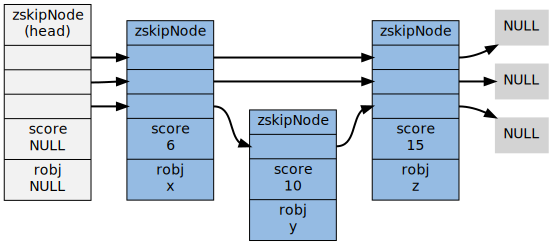
\includegraphics{graphviz-ba063df77d0d9a6581ef14368644db453ab8a7f7.pdf}

为了展示的方便,
在图片中我们直接将 \code{member} 和 \code{score} 值包含在表节点中,
但是在实际的定义中,
因为跳跃表要和另一个实现有序集的结构(字典)分享 \code{member} 和 \code{score} 值,
所以跳跃表只保存指向 \code{member} 和 \code{score} 的指针。
更详细的信息,请参考《{\hyperref[datatype/sorted_set:sorted-set-chapter]{\emph{有序集}}}》章节。


\subsection{小结}
\label{internal-datastruct/skiplist:id5}\begin{itemize}
\item {} 
跳跃表是一种随机化数据结构,它的查找、添加、删除操作都可以在对数期望时间下完成。

\item {} 
跳跃表目前在 Redis 的唯一作用就是作为有序集类型的底层数据结构(之一,另一个构成有序集的结构是字典)。

\item {} 
为了适应自身的需求,Redis 基于 William Pugh 论文中描述的跳跃表进行了修改,包括:
\begin{enumerate}
\item {} 
\code{score} 值可重复。

\item {} 
对比一个元素需要同时检查它的 \code{score} 和 \code{memeber} 。

\item {} 
每个节点带有高度为 1 层的后退指针,用于从表尾方向向表头方向迭代。

\end{enumerate}

\end{itemize}


\chapter{内存映射数据结构}
\label{index:id2}
虽然内部数据结构非常强大,
但是创建一系列完整的数据结构本身也是一件相当耗费内存的工作,
当一个对象包含的元素数量并不多,
或者元素本身的体积并不大时,
使用代价高昂的内部数据结构并不是最好的办法。

为了解决这一问题,
Redis 在条件允许的情况下,
会使用内存映射数据结构来代替内部数据结构。

内存映射数据结构是一系列经过特殊编码的字节序列,
创建它们所消耗的内存通常比作用类似的内部数据结构要少得多,
如果使用得当,
内存映射数据结构可以为用户节省大量的内存。

不过,
因为内存映射数据结构的编码和操作方式要比内部数据结构要复杂得多,
所以内存映射数据结构所占用的 CPU 时间会比作用类似的内部数据结构要多。

这一部分将对 Redis 目前正在使用的两种内存映射数据结构进行介绍。


\section{整数集合}
\label{compress-datastruct/intset::doc}\label{compress-datastruct/intset:id1}
整数集合(intset)用于有序、无重复地保存多个整数值,
它会根据元素的值,
自动选择该用什么长度的整数类型来保存元素。

举个例子,
如果在一个 intset 里面,
最长的元素可以用 \code{int16\_t} 类型来保存,
那么这个 intset 的所有元素都以 \code{int16\_t} 类型来保存。

另一方面,
如果有一个新元素要加入到这个 intset ,
并且这个元素不能用 \code{int16\_t} 类型来保存 ——
比如说,
新元素的长度为 \code{int32\_t} ,
那么这个 intset 就会自动进行“升级”:
先将集合中现有的所有元素从 \code{int16\_t}  类型转换为 \code{int32\_t} 类型,
接着再将新元素加入到集合中。

根据需要,
intset 可以自动从 \code{int16\_t} 升级到 \code{int32\_t} 或 \code{int64\_t} ,
或者从 \code{int32\_t} 升级到 \code{int64\_t} 。


\subsection{整数集合的应用}
\label{compress-datastruct/intset:id2}
Intset 是集合键的底层实现之一,如果一个集合:
\begin{enumerate}
\item {} 
只保存着整数元素;

\item {} 
元素的数量不多;

\end{enumerate}

那么 Redis 就会使用 intset 来保存集合元素。

具体的信息请参考《{\hyperref[datatype/set:set-chapter]{\emph{集合}}}》。


\subsection{数据结构和主要操作}
\label{compress-datastruct/intset:id3}
以下是 \code{intset.h/intset} 类型的定义:

\begin{Verbatim}[commandchars=\\\{\}]
\PYG{k}{typedef} \PYG{k}{struct} \PYG{n}{intset} \PYG{p}{\PYGZob{}}

    \PYG{c+c1}{// 保存元素所使用的类型的长度}
    \PYG{k+kt}{uint32\PYGZus{}t} \PYG{n}{encoding}\PYG{p}{;}

    \PYG{c+c1}{// 元素个数}
    \PYG{k+kt}{uint32\PYGZus{}t} \PYG{n}{length}\PYG{p}{;}

    \PYG{c+c1}{// 保存元素的数组}
    \PYG{k+kt}{int8\PYGZus{}t} \PYG{n}{contents}\PYG{p}{[}\PYG{p}{]}\PYG{p}{;}

\PYG{p}{\PYGZcb{}} \PYG{n}{intset}\PYG{p}{;}
\end{Verbatim}

\code{encoding} 的值可以是以下三个常量的其中一个(定义位于 \code{intset.c} ):

\begin{Verbatim}[commandchars=\\\{\}]
\PYG{c+cp}{\PYGZsh{}}\PYG{c+cp}{define INTSET\PYGZus{}ENC\PYGZus{}INT16 (sizeof(int16\PYGZus{}t))}
\PYG{c+cp}{\PYGZsh{}}\PYG{c+cp}{define INTSET\PYGZus{}ENC\PYGZus{}INT32 (sizeof(int32\PYGZus{}t))}
\PYG{c+cp}{\PYGZsh{}}\PYG{c+cp}{define INTSET\PYGZus{}ENC\PYGZus{}INT64 (sizeof(int64\PYGZus{}t))}
\end{Verbatim}

\code{contents} 数组是实际保存元素的地方,数组中的元素有以下两个特性:
\begin{itemize}
\item {} 
没有重复元素;

\item {} 
元素在数组中从小到大排列;

\end{itemize}

\code{contents} 数组的 \code{int8\_t} 类型声明比较容易让人误解,实际上, \code{intset} 并不使用 \code{int8\_t} 类型来保存任何元素,结构中的这个类型声明只是作为一个占位符使用:在对 \code{contents} 中的元素进行读取或者写入时,程序并不是直接使用 \code{contents} 来对元素进行索引,而是根据 \code{encoding} 的值,对 \code{contents} 进行类型转换和指针运算,计算出元素在内存中的正确位置。在添加新元素,进行内存分配时,分配的容量也是由 \code{encoding} 的值决定。

下表列出了处理 \code{intset} 的一些主要操作,以及这些操作的算法复杂度:

\begin{tabulary}{\linewidth}{|L|L|L|}
\hline
\textbf{
操作
} & \textbf{
函数
} & \textbf{
复杂度
}\\\hline

创建 intset
 & 
\code{intsetNew}
 & 
$\theta(1)$
\\\hline

删除 intset
 & 
无
 & 
无
\\\hline

添加新元素(不升级)
 & 
\code{intsetAdd}
 & 
$O(N)$
\\\hline

添加新元素(升级)
 & 
\code{intsetUpgradeAndAdd}
 & 
$O(N)$
\\\hline

按索引获取元素
 & 
\code{\_intsetGet}
 & 
$\theta(1)$
\\\hline

按索引设置元素
 & 
\code{\_intsetSet}
 & 
$\theta(1)$
\\\hline

查找元素,返回索引
 & 
\code{intsetSearch}
 & 
$O(\lg N)$
\\\hline

删除元素
 & 
\code{intsetRemove}
 & 
$O(N)$
\\\hline
\end{tabulary}



\subsection{intset 运行实例}
\label{compress-datastruct/intset:intset}
让我们跟踪一个 \code{intset} 的创建和添加过程,籍此了解 \code{intset} 的运作方式。


\subsubsection{创建新 intset}
\label{compress-datastruct/intset:id4}
\code{intset.c/intsetNew} 函数创建一个新的 \code{intset} ,并为它设置初始化值:

\begin{Verbatim}[commandchars=\\\{\}]
\PYG{n}{intset} \PYG{o}{*}\PYG{n}{is} \PYG{o}{=} \PYG{n}{intsetNew}\PYG{p}{(}\PYG{p}{)}\PYG{p}{;}

\PYG{c+c1}{// intset-\PYGZgt{}encoding = INTSET\PYGZus{}ENC\PYGZus{}INT16;}
\PYG{c+c1}{// intset-\PYGZgt{}length 0;}
\PYG{c+c1}{// intset-\PYGZgt{}contents = [];}
\end{Verbatim}

注意 \code{encoding} 使用 \code{INTSET\_ENC\_INT16} 作为初始值。


\subsubsection{添加新元素到 intset}
\label{compress-datastruct/intset:id5}
创建 \code{intset} 之后,就可以对它添加新元素了。

添加新元素到 \code{intset} 的工作由 \code{intset.c/intsetAdd} 函数完成,它需要处理以下三种情况:
\begin{enumerate}
\item {} 
元素已存在于集合,不做动作;

\item {} 
元素不存在于集合,并且添加新元素并不需要升级;

\item {} 
元素不存在于集合,但是要在升级之后,才能添加新元素;

\end{enumerate}

并且,
\code{intsetAdd} 需要维持 \code{intset-\textgreater{}contents} 的以下性质:
\begin{enumerate}
\item {} 
确保数组中没有重复元素;

\item {} 
确保数组中的元素按从小到大排序;

\end{enumerate}

整个 \code{intsetAdd} 的执行流程可以表示为下图:

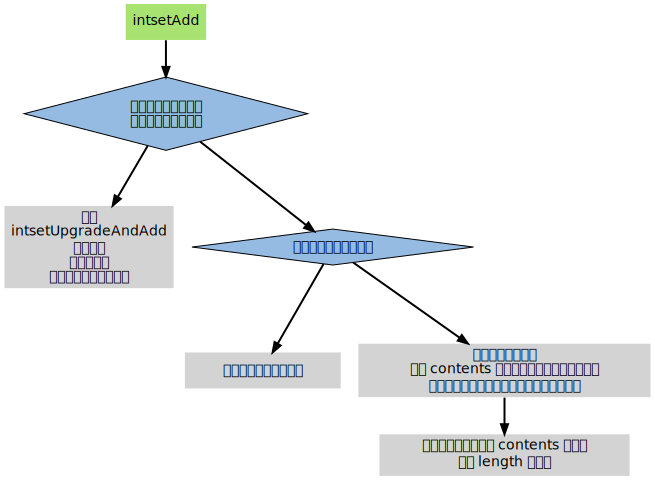
\includegraphics{graphviz-1565e65522fdcd4245030f17b5074729033297d8.pdf}

以下两个小节分别演示添加操作在升级和不升级两种情况下的执行过程。


\subsubsection{添加新元素到 intset (不需要升级)}
\label{compress-datastruct/intset:id6}
如果 intset 现有的编码方式适用于新元素,
那么可以直接将新元素添加到 intset ,
无须对 intset 进行升级。

以下代码演示了将三个 \code{int16\_t} 类型的整数添加到集合的过程,
以及在添加过程中,集合的状态:

\begin{Verbatim}[commandchars=\\\{\}]
\PYG{n}{intset} \PYG{o}{*}\PYG{n}{is} \PYG{o}{=} \PYG{n}{intsetNew}\PYG{p}{(}\PYG{p}{)}\PYG{p}{;}

\PYG{n}{intsetAdd}\PYG{p}{(}\PYG{n}{is}\PYG{p}{,} \PYG{l+m+mi}{10}\PYG{p}{,} \PYG{n+nb}{NULL}\PYG{p}{)}\PYG{p}{;}

\PYG{c+c1}{// is-\PYGZgt{}encoding = INTSET\PYGZus{}ENC\PYGZus{}INT16;}
\PYG{c+c1}{// is-\PYGZgt{}length = 1;}
\PYG{c+c1}{// is-\PYGZgt{}contents = [10];}

\PYG{n}{intsetAdd}\PYG{p}{(}\PYG{n}{is}\PYG{p}{,} \PYG{l+m+mi}{5}\PYG{p}{,} \PYG{n+nb}{NULL}\PYG{p}{)}\PYG{p}{;}

\PYG{c+c1}{// is-\PYGZgt{}encoding = INTSET\PYGZus{}ENC\PYGZus{}INT16;}
\PYG{c+c1}{// is-\PYGZgt{}length = 2;}
\PYG{c+c1}{// is-\PYGZgt{}contents = [5, 10];}

\PYG{n}{intsetAdd}\PYG{p}{(}\PYG{n}{is}\PYG{p}{,} \PYG{l+m+mi}{12}\PYG{p}{,} \PYG{n+nb}{NULL}\PYG{p}{)}\PYG{p}{;}

\PYG{c+c1}{// is-\PYGZgt{}encoding = INTSET\PYGZus{}ENC\PYGZus{}INT16;}
\PYG{c+c1}{// is-\PYGZgt{}length = 3;}
\PYG{c+c1}{// is-\PYGZgt{}contents = [5, 10, 12]}
\end{Verbatim}

因为添加的三个元素都可以表示为 \code{int16\_t} ,
因此 \code{is-\textgreater{}encoding} 一直都是 \code{INTSET\_ENC\_INT16} 。

另一方面, \code{is-\textgreater{}length} 和 \code{is-\textgreater{}contents} 的值则随着新元素的加入而被修改。


\subsubsection{添加新元素到 intset (需要升级)}
\label{compress-datastruct/intset:id7}
当要添加新元素到 intset ,并且 intset 当前的编码并不适用于新元素的编码时,就需要对 inset 进行升级。

以下代码演示了带升级的添加操作的执行过程:

\begin{Verbatim}[commandchars=\\\{\}]
\PYG{n}{intset} \PYG{o}{*}\PYG{n}{is} \PYG{o}{=} \PYG{n}{intsetNew}\PYG{p}{(}\PYG{p}{)}\PYG{p}{;}

\PYG{n}{intsetAdd}\PYG{p}{(}\PYG{n}{is}\PYG{p}{,} \PYG{l+m+mi}{1}\PYG{p}{,} \PYG{n+nb}{NULL}\PYG{p}{)}\PYG{p}{;}

\PYG{c+c1}{// is-\PYGZgt{}encoding = INTSET\PYGZus{}ENC\PYGZus{}INT16;}
\PYG{c+c1}{// is-\PYGZgt{}length = 1;}
\PYG{c+c1}{// is-\PYGZgt{}contents = [1];                  // 所有值使用 int16\PYGZus{}t 保存}

\PYG{n}{intsetAdd}\PYG{p}{(}\PYG{n}{is}\PYG{p}{,} \PYG{l+m+mi}{65535}\PYG{p}{,} \PYG{n+nb}{NULL}\PYG{p}{)}\PYG{p}{;}

\PYG{c+c1}{// is-\PYGZgt{}encoding = INTSET\PYGZus{}ENC\PYGZus{}INT32;     // 升级}
\PYG{c+c1}{// is-\PYGZgt{}length = 2;}
\PYG{c+c1}{// is-\PYGZgt{}contents = [1, 65535];           // 所有值使用 int32\PYGZus{}t 保存}

\PYG{n}{intsetAdd}\PYG{p}{(}\PYG{n}{is}\PYG{p}{,} \PYG{l+m+mi}{70000}\PYG{p}{,} \PYG{n+nb}{NULL}\PYG{p}{)}\PYG{p}{;}

\PYG{c+c1}{// is-\PYGZgt{}encoding = INTSET\PYGZus{}ENC\PYGZus{}INT32;}
\PYG{c+c1}{// is-\PYGZgt{}length = 3;}
\PYG{c+c1}{// is-\PYGZgt{}contents = [1, 65535, 70000];}

\PYG{n}{intsetAdd}\PYG{p}{(}\PYG{n}{is}\PYG{p}{,} \PYG{l+m+mi}{4294967295}\PYG{p}{,} \PYG{n+nb}{NULL}\PYG{p}{)}\PYG{p}{;}

\PYG{c+c1}{// is-\PYGZgt{}encoding = INTSET\PYGZus{}ENC\PYGZus{}INT64;                 // 升级}
\PYG{c+c1}{// is-\PYGZgt{}length = 4;}
\PYG{c+c1}{// is-\PYGZgt{}contents = [1, 65535, 70000, 4294967295];    // 所有值使用 int64\PYGZus{}t 保存}
\end{Verbatim}

在添加 \code{65535} 和 \code{4294967295} 之后,
\code{encoding} 属性的值,以及 \code{contents} 数组保存值的方式,都被改变了。


\subsection{升级}
\label{compress-datastruct/intset:id8}
在添加新元素时,如果 \code{intsetAdd} 发现新元素不能用现有的编码方式来保存,它就会将升级集合和添加新元素的任务转交给 \code{intsetUpgradeAndAdd} 来完成:

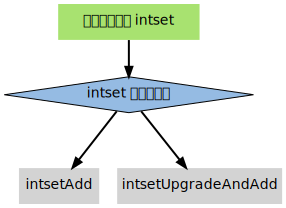
\includegraphics{graphviz-1058591c9a0d517a84afc9e1e5e90aa88e27fc1a.pdf}

\code{intsetUpgradeAndAdd} 需要完成以下几个任务:
\begin{enumerate}
\item {} 
对新元素进行检测,看保存这个新元素需要什么类型的编码;

\item {} 
将集合 \code{encoding} 属性的值设置为新编码类型,并根据新编码类型,对整个 \code{contents} 数组进行内存重分配。

\item {} 
调整 \code{contents} 数组内原有元素在内存中的排列方式,让它们从旧编码调整为新编码。

\item {} 
将新元素添加到集合中。

\end{enumerate}

整个过程中,最复杂的就是第三步,让我们用一个例子来理解这个步骤。


\subsubsection{升级实例}
\label{compress-datastruct/intset:id9}
假设有一个 \code{intset} ,里面包含三个用 \code{int16\_t} 方式保存的数值,分别是 \code{1} 、 \code{2} 和 \code{3} ,它的结构如下:

\begin{Verbatim}[commandchars=\\\{\}]
\PYG{n}{intset}\PYG{o}{-}\PYG{o}{\PYGZgt{}}\PYG{n}{encoding} \PYG{o}{=} \PYG{n}{INTSET\PYGZus{}ENC\PYGZus{}INT16}\PYG{p}{;}
\PYG{n}{intset}\PYG{o}{-}\PYG{o}{\PYGZgt{}}\PYG{n}{length} \PYG{o}{=} \PYG{l+m+mi}{3}\PYG{p}{;}
\PYG{n}{intset}\PYG{o}{-}\PYG{o}{\PYGZgt{}}\PYG{n}{contents} \PYG{o}{=} \PYG{p}{[}\PYG{l+m+mi}{1}\PYG{p}{,} \PYG{l+m+mi}{2}\PYG{p}{,} \PYG{l+m+mi}{3}\PYG{p}{]}\PYG{p}{;}
\end{Verbatim}

其中, \code{intset-\textgreater{}contents} 在内存中的排列如下:

\begin{Verbatim}[commandchars=\\\{\}]
\PYG{n}{bit}     \PYG{l+m+mi}{0}    \PYG{l+m+mi}{15}    \PYG{l+m+mi}{31}    \PYG{l+m+mi}{47}
\PYG{n}{value}   \PYG{o}{\textbar{}}  \PYG{l+m+mi}{1}  \PYG{o}{\textbar{}}  \PYG{l+m+mi}{2}  \PYG{o}{\textbar{}}  \PYG{l+m+mi}{3}  \PYG{o}{\textbar{}}
\end{Verbatim}

现在,我们要要将一个长度为 \code{int32\_t} 的值 \code{65535} 加入到集合中, \code{intset} 需要执行以下步骤:
\begin{enumerate}
\item {} 
将 \code{encoding} 属性设置为 \code{INTSET\_ENC\_INT32} 。

\item {} 
根据 \code{encoding} 属性的值,对 \code{contents} 数组进行内存重分配。

重分配完成之后, \code{contents} 在内存中的排列如下:

\begin{Verbatim}[commandchars=\\\{\}]
\PYG{n}{bit}     \PYG{l+m+mi}{0}    \PYG{l+m+mi}{15}    \PYG{l+m+mi}{31}    \PYG{l+m+mi}{47}     \PYG{l+m+mi}{63}        \PYG{l+m+mi}{95}       \PYG{l+m+mi}{127}
\PYG{n}{value}   \PYG{o}{\textbar{}}  \PYG{l+m+mi}{1}  \PYG{o}{\textbar{}}  \PYG{l+m+mi}{2}  \PYG{o}{\textbar{}}  \PYG{l+m+mi}{3}  \PYG{o}{\textbar{}}  \PYG{o}{?}  \PYG{o}{\textbar{}}    \PYG{o}{?}    \PYG{o}{\textbar{}}    \PYG{o}{?}    \PYG{o}{\textbar{}}
\end{Verbatim}

\code{contents} 数组现在共有可容纳 4 个 \code{int32\_t} 值的空间。

\item {} 
因为原来的 3 个 \code{int16\_t} 值还“挤在” \code{contents} 前面的 48 个位里, 所以程序需要对它们进行移动和类型转换, 从而让它们适应集合的新编码方式。

首先是移动 \code{3} :

\begin{Verbatim}[commandchars=\\\{\}]
\PYG{n}{bit}     \PYG{l+m+mi}{0}    \PYG{l+m+mi}{15}    \PYG{l+m+mi}{31}    \PYG{l+m+mi}{47}     \PYG{l+m+mi}{63}        \PYG{l+m+mi}{95}       \PYG{l+m+mi}{127}
\PYG{n}{value}   \PYG{o}{\textbar{}}  \PYG{l+m+mi}{1}  \PYG{o}{\textbar{}}  \PYG{l+m+mi}{2}  \PYG{o}{\textbar{}}  \PYG{l+m+mi}{3}  \PYG{o}{\textbar{}}  \PYG{o}{?}  \PYG{o}{\textbar{}}    \PYG{l+m+mi}{3}    \PYG{o}{\textbar{}}    \PYG{o}{?}    \PYG{o}{\textbar{}}
                       \PYG{o}{\textbar{}}             \PYG{o}{\PYGZca{}}
                       \PYG{o}{\textbar{}}             \PYG{o}{\textbar{}}
                       \PYG{o}{+}\PYG{o}{-}\PYG{o}{-}\PYG{o}{-}\PYG{o}{-}\PYG{o}{-}\PYG{o}{-}\PYG{o}{-}\PYG{o}{-}\PYG{o}{-}\PYG{o}{-}\PYG{o}{-}\PYG{o}{-}\PYG{o}{-}\PYG{o}{+}
                     \PYG{k+kt}{int16\PYGZus{}t} \PYG{o}{-}\PYG{o}{\PYGZgt{}} \PYG{k+kt}{int32\PYGZus{}t}
\end{Verbatim}

接着移动 \code{2} :

\begin{Verbatim}[commandchars=\\\{\}]
\PYG{n}{bit}     \PYG{l+m+mi}{0}    \PYG{l+m+mi}{15}    \PYG{l+m+mi}{31}   \PYG{l+m+mi}{47}     \PYG{l+m+mi}{63}        \PYG{l+m+mi}{95}       \PYG{l+m+mi}{127}
\PYG{n}{value}   \PYG{o}{\textbar{}}  \PYG{l+m+mi}{1}  \PYG{o}{\textbar{}}  \PYG{l+m+mi}{2}  \PYG{o}{\textbar{}}    \PYG{l+m+mi}{2}     \PYG{o}{\textbar{}}    \PYG{l+m+mi}{3}    \PYG{o}{\textbar{}}    \PYG{o}{?}    \PYG{o}{\textbar{}}
                 \PYG{o}{\textbar{}}       \PYG{o}{\PYGZca{}}
                 \PYG{o}{\textbar{}}       \PYG{o}{\textbar{}}
                 \PYG{o}{+}\PYG{o}{-}\PYG{o}{-}\PYG{o}{-}\PYG{o}{-}\PYG{o}{-}\PYG{o}{-}\PYG{o}{-}\PYG{o}{+}
            \PYG{k+kt}{int16\PYGZus{}t} \PYG{o}{-}\PYG{o}{\PYGZgt{}} \PYG{k+kt}{int32\PYGZus{}t}
\end{Verbatim}

最后,移动 \code{1} :

\begin{Verbatim}[commandchars=\\\{\}]
\PYG{n}{bit}     \PYG{l+m+mi}{0}   \PYG{l+m+mi}{15}    \PYG{l+m+mi}{31}   \PYG{l+m+mi}{47}     \PYG{l+m+mi}{63}        \PYG{l+m+mi}{95}       \PYG{l+m+mi}{127}
\PYG{n}{value}   \PYG{o}{\textbar{}}    \PYG{l+m+mi}{1}     \PYG{o}{\textbar{}}    \PYG{l+m+mi}{2}     \PYG{o}{\textbar{}}    \PYG{l+m+mi}{3}    \PYG{o}{\textbar{}}    \PYG{o}{?}    \PYG{o}{\textbar{}}
            \PYG{o}{\textbar{}} \PYG{o}{\PYGZca{}}
            \PYG{n}{V} \PYG{o}{\textbar{}}
    \PYG{k+kt}{int16\PYGZus{}t} \PYG{o}{-}\PYG{o}{\PYGZgt{}} \PYG{k+kt}{int32\PYGZus{}t}
\end{Verbatim}

\item {} 
最后,将新值 65535 添加到数组:

\begin{Verbatim}[commandchars=\\\{\}]
\PYG{n}{bit}     \PYG{l+m+mi}{0}   \PYG{l+m+mi}{15}    \PYG{l+m+mi}{31}   \PYG{l+m+mi}{47}     \PYG{l+m+mi}{63}        \PYG{l+m+mi}{95}       \PYG{l+m+mi}{127}
\PYG{n}{value}   \PYG{o}{\textbar{}}    \PYG{l+m+mi}{1}     \PYG{o}{\textbar{}}    \PYG{l+m+mi}{2}     \PYG{o}{\textbar{}}    \PYG{l+m+mi}{3}    \PYG{o}{\textbar{}}  \PYG{l+m+mi}{65535}  \PYG{o}{\textbar{}}
                                             \PYG{o}{\PYGZca{}}
                                             \PYG{o}{\textbar{}}
                                            \PYG{n}{add}
\end{Verbatim}

将 \code{intset-\textgreater{}length} 设置为 \code{4} 。

\end{enumerate}

至此,集合的升级和添加操作完成,现在的 \code{intset} 结构如下:

\begin{Verbatim}[commandchars=\\\{\}]
\PYG{n}{intset}\PYG{o}{-}\PYG{o}{\PYGZgt{}}\PYG{n}{encoding} \PYG{o}{=} \PYG{n}{INTSET\PYGZus{}ENC\PYGZus{}INT32}\PYG{p}{;}
\PYG{n}{intset}\PYG{o}{-}\PYG{o}{\PYGZgt{}}\PYG{n}{length} \PYG{o}{=} \PYG{l+m+mi}{4}\PYG{p}{;}
\PYG{n}{intset}\PYG{o}{-}\PYG{o}{\PYGZgt{}}\PYG{n}{contents} \PYG{o}{=} \PYG{p}{[}\PYG{l+m+mi}{1}\PYG{p}{,} \PYG{l+m+mi}{2}\PYG{p}{,} \PYG{l+m+mi}{3}\PYG{p}{,} \PYG{l+m+mi}{65535}\PYG{p}{]}\PYG{p}{;}
\end{Verbatim}


\subsection{关于升级}
\label{compress-datastruct/intset:id10}
关于升级操作,还有两点需要提醒一下:


\subsubsection{第一,从较短整数到较长整数的转换,并不会更改元素里面的值。}
\label{compress-datastruct/intset:id11}
在 C 语言中,从长度较短的带符号整数到长度较长的带符号整数之间的转换(比如从 \code{int16\_t} 转换为 \code{int32\_t} )总是可行的(不会溢出)、无损的。

另一方面,从较长整数到较短整数之间的转换可能是有损的(比如从 \code{int32\_t} 转换为 \code{int16\_t} )。

因为 intset 只进行从较短整数到较长整数的转换(也即是,只“升级”,不“降级”),因此,“升级”操作并不会修改元素原有的值。


\subsubsection{第二,集合编码元素的方式,由元素中长度最大的那个值来决定。}
\label{compress-datastruct/intset:id12}
就像前面演示的例子一样,
当要将一个 \code{int32\_t} 编码的新元素添加到集合时,
集合原有的所有 \code{int16\_t} 编码的元素,
都必须转换为 \code{int32\_t} 。

尽管这个集合真正需要用 \code{int32\_t} 长度来保存的元素只有一个,
但整个集合的所有元素都必须转换为这种类型。


\subsection{关于元素移动}
\label{compress-datastruct/intset:id13}
在进行升级的过程中,需要对数组内的元素进行“类型转换”和“移动”操作。

其中,
移动不仅出现在升级(\code{intsetUpgradeAndAdd})操作中,
还出现其他对 \code{contents} 数组内容进行增删的操作上,
比如 \code{intsetAdd} 和 \code{intsetRemove} ,
因为这种移动操作需要处理 intset 中的所有元素,
所以这些函数的复杂度都不低于 $O(N)$ 。


\subsection{其他操作}
\label{compress-datastruct/intset:id14}
以下是一些关于 intset 其他操作的讨论。


\subsubsection{读取}
\label{compress-datastruct/intset:id15}
有两种方式读取 \code{intset} 的元素,一种是 \code{\_intsetGet} ,另一种是 \code{intsetSearch} :
\begin{itemize}
\item {} 
\code{\_intsetGet} 接受一个给定的索引 \code{pos} ,并根据 \code{intset-\textgreater{}encoding} 的值进行指针运算,计算出给定索引在 \code{intset-\textgreater{}contents} 数组上的值。

\item {} 
\code{intsetSearch} 则使用\href{http://en.wikipedia.org/wiki/Binary\_search\_algorithm}{二分查找}算法,判断一个给定元素在 \code{contents} 数组上的索引。

\end{itemize}


\subsubsection{写入}
\label{compress-datastruct/intset:id17}
除了前面介绍过的 \code{intsetAdd} 和 \code{intsetUpgradeAndAdd} 之外, \code{\_intsetSet} 也对集合进行写入操作:
它接受一个索引 \code{pos} ,以及一个 \code{new\_value} ,将 \code{contents} 数组 \code{pos} 位置的值设为 \code{new\_value} 。


\subsubsection{删除}
\label{compress-datastruct/intset:id18}
删除单个元素的工作由 \code{intsetRemove} 操作,
它先调用 \code{intsetSearch} 找到需要被删除的元素在 \code{contents} 数组中的索引,
然后使用内存移位操作,将目标元素从内存中抹去,
最后,通过内存重分配,对 \code{contents} 数组的长度进行调整。


\subsubsection{降级}
\label{compress-datastruct/intset:id19}
Intset 不支持降级操作。

Intset 定位为一种受限的中间表示,
只能保存整数值,
而且元素的个数也不能超过 \code{redis.h/REDIS\_SET\_MAX\_INTSET\_ENTRIES} (目前版本值为 \code{512} )
这些条件决定了它被保存的时间不会太长,
因此对它进行太复杂的操作,
没有必要。

当然,如果内存确实十分紧张的话,给 intset 添加降级功能也是可以实现的,不过这可能会让 \code{intset} 的代码增长一倍。


\subsection{小结}
\label{compress-datastruct/intset:id20}\begin{itemize}
\item {} 
Intset 用于有序、无重复地保存多个整数值,它会根据元素的值,自动选择该用什么长度的整数类型来保存元素。

\item {} 
当一个位长度更长的整数值添加到 intset 时,需要对 intset 进行升级,新 intset 中每个元素的位长度都等于新添加值的位长度,但原有元素的值不变。

\item {} 
升级会引起整个 intset 进行内存重分配,并移动集合中的所有元素,这个操作的复杂度为 $O(N)$ 。

\item {} 
Intset 只支持升级,不支持降级。

\item {} 
Intset 是有序的,程序使用二分查找算法来实现查找操作,复杂度为 $O(\lg N)$ 。

\end{itemize}


\section{压缩列表}
\label{compress-datastruct/ziplist:ziplist-chapter}\label{compress-datastruct/ziplist::doc}\label{compress-datastruct/ziplist:id1}
Ziplist 是由一系列特殊编码的内存块构成的列表,
一个 ziplist 可以包含多个节点(entry),
每个节点可以保存一个长度受限的字符数组(不以 \code{\textbackslash{}0} 结尾的 \code{char} 数组)或者整数,
包括:
\begin{itemize}
\item {} \begin{description}
\item[{字符数组}] \leavevmode\begin{itemize}
\item {} 
长度小于等于 \code{63} ($2^{6}-1$)字节的字符数组

\item {} 
长度小于等于 \code{16383} ($2^{14}-1$) 字节的字符数组

\item {} 
长度小于等于 \code{4294967295} ($2^{32}-1$)字节的字符数组

\end{itemize}

\end{description}

\item {} \begin{description}
\item[{整数}] \leavevmode\begin{itemize}
\item {} 
\code{4} 位长,介于 \code{0} 至 \code{12} 之间的无符号整数

\item {} 
\code{1} 字节长,有符号整数

\item {} 
\code{3} 字节长,有符号整数

\item {} 
\code{int16\_t} 类型整数

\item {} 
\code{int32\_t} 类型整数

\item {} 
\code{int64\_t} 类型整数

\end{itemize}

\end{description}

\end{itemize}

因为 ziplist 节约内存的性质,
它被哈希键、列表键和有序集合键作为初始化的底层实现来使用,
更多信息请参考《{\hyperref[datatype/hash:hash-chapter]{\emph{哈希表}}}》、《{\hyperref[datatype/list:list-chapter]{\emph{列表}}}》和《{\hyperref[datatype/sorted_set:sorted-set-chapter]{\emph{有序集}}}》章节。

本章先介绍 ziplist 的组成结构,
以及 ziplist 节点的编码方式,
然后介绍 ziplist 的添加操作和删除操作的执行过程,
以及这两种操作可能引起的连锁更新现象,
最后介绍 ziplist 的遍历方法和节点查找方式。


\subsection{ziplist 的构成}
\label{compress-datastruct/ziplist:ziplist}
下图展示了一个 ziplist 的典型分布结构:

\begin{Verbatim}[commandchars=\\\{\}]
\PYG{n}{area}        \PYG{o}{\textbar{}}\PYG{o}{\PYGZlt{}}\PYG{o}{-}\PYG{o}{-}\PYG{o}{-}\PYG{o}{-} \PYG{n}{ziplist} \PYG{n}{header} \PYG{o}{-}\PYG{o}{-}\PYG{o}{-}\PYG{o}{-}\PYG{o}{\PYGZgt{}}\PYG{o}{\textbar{}}\PYG{o}{\PYGZlt{}}\PYG{o}{-}\PYG{o}{-}\PYG{o}{-}\PYG{o}{-}\PYG{o}{-}\PYG{o}{-}\PYG{o}{-}\PYG{o}{-}\PYG{o}{-}\PYG{o}{-}\PYG{o}{-} \PYG{n}{entries} \PYG{o}{-}\PYG{o}{-}\PYG{o}{-}\PYG{o}{-}\PYG{o}{-}\PYG{o}{-}\PYG{o}{-}\PYG{o}{-}\PYG{o}{-}\PYG{o}{-}\PYG{o}{-}\PYG{o}{-}\PYG{o}{-}\PYG{o}{\PYGZgt{}}\PYG{o}{\textbar{}}\PYG{o}{\PYGZlt{}}\PYG{o}{-}\PYG{n}{end}\PYG{o}{-}\PYG{o}{\PYGZgt{}}\PYG{o}{\textbar{}}

\PYG{n}{size}          \PYG{l+m+mi}{4} \PYG{n}{bytes}  \PYG{l+m+mi}{4} \PYG{n}{bytes}  \PYG{l+m+mi}{2} \PYG{n}{bytes}    \PYG{o}{?}        \PYG{o}{?}        \PYG{o}{?}        \PYG{o}{?}     \PYG{l+m+mi}{1} \PYG{n}{byte}
            \PYG{o}{+}\PYG{o}{-}\PYG{o}{-}\PYG{o}{-}\PYG{o}{-}\PYG{o}{-}\PYG{o}{-}\PYG{o}{-}\PYG{o}{-}\PYG{o}{-}\PYG{o}{+}\PYG{o}{-}\PYG{o}{-}\PYG{o}{-}\PYG{o}{-}\PYG{o}{-}\PYG{o}{-}\PYG{o}{-}\PYG{o}{-}\PYG{o}{+}\PYG{o}{-}\PYG{o}{-}\PYG{o}{-}\PYG{o}{-}\PYG{o}{-}\PYG{o}{-}\PYG{o}{-}\PYG{o}{+}\PYG{o}{-}\PYG{o}{-}\PYG{o}{-}\PYG{o}{-}\PYG{o}{-}\PYG{o}{-}\PYG{o}{-}\PYG{o}{-}\PYG{o}{+}\PYG{o}{-}\PYG{o}{-}\PYG{o}{-}\PYG{o}{-}\PYG{o}{-}\PYG{o}{-}\PYG{o}{-}\PYG{o}{-}\PYG{o}{+}\PYG{o}{-}\PYG{o}{-}\PYG{o}{-}\PYG{o}{-}\PYG{o}{-}\PYG{o}{-}\PYG{o}{-}\PYG{o}{-}\PYG{o}{+}\PYG{o}{-}\PYG{o}{-}\PYG{o}{-}\PYG{o}{-}\PYG{o}{-}\PYG{o}{-}\PYG{o}{-}\PYG{o}{-}\PYG{o}{+}\PYG{o}{-}\PYG{o}{-}\PYG{o}{-}\PYG{o}{-}\PYG{o}{-}\PYG{o}{-}\PYG{o}{-}\PYG{o}{+}
\PYG{n}{component}   \PYG{o}{\textbar{}} \PYG{n}{zlbytes} \PYG{o}{\textbar{}} \PYG{n}{zltail} \PYG{o}{\textbar{}} \PYG{n}{zllen} \PYG{o}{\textbar{}} \PYG{n}{entry1} \PYG{o}{\textbar{}} \PYG{n}{entry2} \PYG{o}{\textbar{}}  \PYG{p}{.}\PYG{p}{.}\PYG{p}{.}   \PYG{o}{\textbar{}} \PYG{n}{entryN} \PYG{o}{\textbar{}} \PYG{n}{zlend} \PYG{o}{\textbar{}}
            \PYG{o}{+}\PYG{o}{-}\PYG{o}{-}\PYG{o}{-}\PYG{o}{-}\PYG{o}{-}\PYG{o}{-}\PYG{o}{-}\PYG{o}{-}\PYG{o}{-}\PYG{o}{+}\PYG{o}{-}\PYG{o}{-}\PYG{o}{-}\PYG{o}{-}\PYG{o}{-}\PYG{o}{-}\PYG{o}{-}\PYG{o}{-}\PYG{o}{+}\PYG{o}{-}\PYG{o}{-}\PYG{o}{-}\PYG{o}{-}\PYG{o}{-}\PYG{o}{-}\PYG{o}{-}\PYG{o}{+}\PYG{o}{-}\PYG{o}{-}\PYG{o}{-}\PYG{o}{-}\PYG{o}{-}\PYG{o}{-}\PYG{o}{-}\PYG{o}{-}\PYG{o}{+}\PYG{o}{-}\PYG{o}{-}\PYG{o}{-}\PYG{o}{-}\PYG{o}{-}\PYG{o}{-}\PYG{o}{-}\PYG{o}{-}\PYG{o}{+}\PYG{o}{-}\PYG{o}{-}\PYG{o}{-}\PYG{o}{-}\PYG{o}{-}\PYG{o}{-}\PYG{o}{-}\PYG{o}{-}\PYG{o}{+}\PYG{o}{-}\PYG{o}{-}\PYG{o}{-}\PYG{o}{-}\PYG{o}{-}\PYG{o}{-}\PYG{o}{-}\PYG{o}{-}\PYG{o}{+}\PYG{o}{-}\PYG{o}{-}\PYG{o}{-}\PYG{o}{-}\PYG{o}{-}\PYG{o}{-}\PYG{o}{-}\PYG{o}{+}
                                       \PYG{o}{\PYGZca{}}                          \PYG{o}{\PYGZca{}}        \PYG{o}{\PYGZca{}}
\PYG{n}{address}                                \PYG{o}{\textbar{}}                          \PYG{o}{\textbar{}}        \PYG{o}{\textbar{}}
                                \PYG{n}{ZIPLIST\PYGZus{}ENTRY\PYGZus{}HEAD}                \PYG{o}{\textbar{}} \PYG{n}{ZIPLIST\PYGZus{}ENTRY\PYGZus{}END}
                                                                  \PYG{o}{\textbar{}}
                                                         \PYG{n}{ZIPLIST\PYGZus{}ENTRY\PYGZus{}TAIL}
\end{Verbatim}

图中各个域的作用如下:

\begin{tabulary}{\linewidth}{|p{2cm}|p{2cm}|p{10.5cm}|}
\hline
\textbf{
域
} & \textbf{
长度/类型
} & \textbf{
域的值
}\\\hline

\code{zlbytes}
 & 
\code{uint32\_t}
 & 
整个 ziplist 占用的内存字节数,对 ziplist 进行内存重分配,或者计算末端时使用。
\\\hline

\code{zltail}
 & 
\code{uint32\_t}
 & 
到达 ziplist 表尾节点的偏移量。
通过这个偏移量,可以在不遍历整个 ziplist 的前提下,弹出表尾节点。
\\\hline

\code{zllen}
 & 
\code{uint16\_t}
 & 
ziplist 中节点的数量。
当这个值小于 \code{UINT16\_MAX} (\code{65535})时,这个值就是 ziplist 中节点的数量;
当这个值等于 \code{UINT16\_MAX} 时,节点的数量需要遍历整个 ziplist 才能计算得出。
\\\hline

\code{entryX}
 & 
\code{?}
 & 
ziplist 所保存的节点,各个节点的长度根据内容而定。
\\\hline

\code{zlend}
 & 
\code{uint8\_t}
 & 
\code{255} 的二进制值 \code{1111 1111} (\code{UINT8\_MAX}) ,用于标记 ziplist 的末端。
\\\hline
\end{tabulary}


为了方便地取出 ziplist 的各个域以及一些指针地址, ziplist 模块定义了以下宏:

\begin{tabulary}{\linewidth}{|p{5.5cm}|p{7cm}|L|}
\hline
\textbf{
宏
} & \textbf{
作用
} & \textbf{
算法复杂度
}\\\hline

\code{ZIPLIST\_BYTES(ziplist)}
 & 
取出 \code{zlbytes} 的值
 & 
$\theta(1)$
\\\hline

\code{ZIPLIST\_TAIL\_OFFSET(ziplist)}
 & 
取出 \code{zltail} 的值
 & 
$\theta(1)$
\\\hline

\code{ZIPLIST\_LENGTH(ziplist)}
 & 
取出 \code{zllen} 的值
 & 
$\theta(1)$
\\\hline

\code{ZIPLIST\_HEADER\_SIZE}
 & 
返回 ziplist header 部分的长度,总是固定的 \code{10} 字节
 & 
$\theta(1)$
\\\hline

\code{ZIPLIST\_ENTRY\_HEAD(ziplist)}
 & 
返回到达 ziplist 第一个节点(表头)的地址
 & 
$\theta(1)$
\\\hline

\code{ZIPLIST\_ENTRY\_TAIL(ziplist)}
 & 
返回到达 ziplist 最后一个节点(表尾)的地址
 & 
$\theta(1)$
\\\hline

\code{ZIPLIST\_ENTRY\_END(ziplist)}
 & 
返回 ziplist 的末端,也即是 \code{zlend} 之前的地址
 & 
$\theta(1)$
\\\hline
\end{tabulary}


因为 ziplist header 部分的长度总是固定的(\code{4} 字节 + \code{4} 字节 + \code{2} 字节),
因此将指针移动到表头节点的复杂度为常数时间;
除此之外,
因为表尾节点的地址可以通过 \code{zltail} 计算得出,
因此将指针移动到表尾节点的复杂度也为常数时间。

以下是用于操作 ziplist 的函数:

\begin{tabulary}{\linewidth}{|p{4cm}|p{8.5cm}|L|}
\hline
\textbf{
函数名
} & \textbf{
作用
} & \textbf{
算法复杂度
}\\\hline

\code{ziplistNew}
 & 
创建一个新的 ziplist
 & 
$\theta(1)$
\\\hline

\code{ziplistResize}
 & 
重新调整 ziplist 的内存大小
 & 
$O(N)$
\\\hline

\code{ziplistPush}
 & 
将一个包含给定值的新节点推入 ziplist 的表头或者表尾
 & 
$O(N^2)$
\\\hline

\code{zipEntry}
 & 
取出给定地址上的节点,并将它的属性保存到 \code{zlentry} 结构然后返回
 & 
$\theta(1)$
\\\hline

\code{ziplistInsert}
 & 
将一个包含给定值的新节点插入到给定地址
 & 
$O(N^2)$
\\\hline

\code{ziplistDelete}
 & 
删除给定地址上的节点
 & 
$O(N^2)$
\\\hline

\code{ziplistDeleteRange}
 & 
在给定索引上,连续进行多次删除
 & 
$O(N^2)$
\\\hline

\code{ziplistFind}
 & 
在 ziplist 中查找并返回包含给定值的节点
 & 
$O(N)$
\\\hline

\code{ziplistLen}
 & 
返回 ziplist 保存的节点数量
 & 
$O(N)$
\\\hline

\code{ziplistBlobLen}
 & 
以字节为单位,返回 ziplist 占用的内存大小
 & 
$\theta(1)$
\\\hline
\end{tabulary}


因为 ziplist 由连续的内存块构成,
在最坏情况下,
当 \code{ziplistPush} 、 \code{ziplistDelete} 这类对节点进行增加或删除的函数之后,
程序需要执行一种称为连锁更新的动作来维持 ziplist 结构本身的性质,
所以这些函数的最坏复杂度都为 $O(N^2)$ 。
不过,因为这种最坏情况出现的概率并不高,
所以大可以放心使用 ziplist ,
而不必太担心出现最坏情况。


\subsection{节点的构成}
\label{compress-datastruct/ziplist:id2}
一个 ziplist 可以包含多个节点,每个节点可以划分为以下几个部分:

\begin{Verbatim}[commandchars=\\\{\}]
\PYG{n}{area}        \PYG{o}{\textbar{}}\PYG{o}{\PYGZlt{}}\PYG{o}{-}\PYG{o}{-}\PYG{o}{-}\PYG{o}{-}\PYG{o}{-}\PYG{o}{-}\PYG{o}{-}\PYG{o}{-}\PYG{o}{-}\PYG{o}{-}\PYG{o}{-}\PYG{o}{-}\PYG{o}{-}\PYG{o}{-}\PYG{o}{-}\PYG{o}{-}\PYG{o}{-}\PYG{o}{-}\PYG{o}{-} \PYG{n}{entry} \PYG{o}{-}\PYG{o}{-}\PYG{o}{-}\PYG{o}{-}\PYG{o}{-}\PYG{o}{-}\PYG{o}{-}\PYG{o}{-}\PYG{o}{-}\PYG{o}{-}\PYG{o}{-}\PYG{o}{-}\PYG{o}{-}\PYG{o}{-}\PYG{o}{-}\PYG{o}{-}\PYG{o}{-}\PYG{o}{-}\PYG{o}{-}\PYG{o}{-}\PYG{o}{\PYGZgt{}}\PYG{o}{\textbar{}}

            \PYG{o}{+}\PYG{o}{-}\PYG{o}{-}\PYG{o}{-}\PYG{o}{-}\PYG{o}{-}\PYG{o}{-}\PYG{o}{-}\PYG{o}{-}\PYG{o}{-}\PYG{o}{-}\PYG{o}{-}\PYG{o}{-}\PYG{o}{-}\PYG{o}{-}\PYG{o}{-}\PYG{o}{-}\PYG{o}{-}\PYG{o}{-}\PYG{o}{+}\PYG{o}{-}\PYG{o}{-}\PYG{o}{-}\PYG{o}{-}\PYG{o}{-}\PYG{o}{-}\PYG{o}{-}\PYG{o}{-}\PYG{o}{-}\PYG{o}{-}\PYG{o}{+}\PYG{o}{-}\PYG{o}{-}\PYG{o}{-}\PYG{o}{-}\PYG{o}{-}\PYG{o}{-}\PYG{o}{-}\PYG{o}{-}\PYG{o}{+}\PYG{o}{-}\PYG{o}{-}\PYG{o}{-}\PYG{o}{-}\PYG{o}{-}\PYG{o}{-}\PYG{o}{-}\PYG{o}{-}\PYG{o}{-}\PYG{o}{+}
\PYG{n}{component}   \PYG{o}{\textbar{}} \PYG{n}{pre\PYGZus{}entry\PYGZus{}length} \PYG{o}{\textbar{}} \PYG{n}{encoding} \PYG{o}{\textbar{}} \PYG{n}{length} \PYG{o}{\textbar{}} \PYG{n}{content} \PYG{o}{\textbar{}}
            \PYG{o}{+}\PYG{o}{-}\PYG{o}{-}\PYG{o}{-}\PYG{o}{-}\PYG{o}{-}\PYG{o}{-}\PYG{o}{-}\PYG{o}{-}\PYG{o}{-}\PYG{o}{-}\PYG{o}{-}\PYG{o}{-}\PYG{o}{-}\PYG{o}{-}\PYG{o}{-}\PYG{o}{-}\PYG{o}{-}\PYG{o}{-}\PYG{o}{+}\PYG{o}{-}\PYG{o}{-}\PYG{o}{-}\PYG{o}{-}\PYG{o}{-}\PYG{o}{-}\PYG{o}{-}\PYG{o}{-}\PYG{o}{-}\PYG{o}{-}\PYG{o}{+}\PYG{o}{-}\PYG{o}{-}\PYG{o}{-}\PYG{o}{-}\PYG{o}{-}\PYG{o}{-}\PYG{o}{-}\PYG{o}{-}\PYG{o}{+}\PYG{o}{-}\PYG{o}{-}\PYG{o}{-}\PYG{o}{-}\PYG{o}{-}\PYG{o}{-}\PYG{o}{-}\PYG{o}{-}\PYG{o}{-}\PYG{o}{+}
\end{Verbatim}

以下几个小节将分别对这个四个部分进行介绍。


\subsubsection{pre\_entry\_length}
\label{compress-datastruct/ziplist:pre-entry-length}
\code{pre\_entry\_length} 记录了前一个节点的长度,通过这个值,可以进行指针计算,从而跳转到上一个节点。

\begin{Verbatim}[commandchars=\\\{\}]
\PYG{n}{area}        \PYG{o}{\textbar{}}\PYG{o}{\PYGZlt{}}\PYG{o}{-}\PYG{o}{-}\PYG{o}{-}\PYG{o}{-} \PYG{n}{previous} \PYG{n}{entry} \PYG{o}{-}\PYG{o}{-}\PYG{o}{-}\PYG{o}{\PYGZgt{}}\PYG{o}{\textbar{}}\PYG{o}{\PYGZlt{}}\PYG{o}{-}\PYG{o}{-}\PYG{o}{-}\PYG{o}{-}\PYG{o}{-}\PYG{o}{-}\PYG{o}{-}\PYG{o}{-}\PYG{o}{-}\PYG{o}{-}\PYG{o}{-}\PYG{o}{-}\PYG{o}{-}\PYG{o}{-}\PYG{o}{-} \PYG{n}{current} \PYG{n}{entry} \PYG{o}{-}\PYG{o}{-}\PYG{o}{-}\PYG{o}{-}\PYG{o}{-}\PYG{o}{-}\PYG{o}{-}\PYG{o}{-}\PYG{o}{-}\PYG{o}{-}\PYG{o}{-}\PYG{o}{-}\PYG{o}{-}\PYG{o}{-}\PYG{o}{-}\PYG{o}{-}\PYG{o}{\PYGZgt{}}\PYG{o}{\textbar{}}

\PYG{n}{size}          \PYG{l+m+mi}{5} \PYG{n}{bytes}                   \PYG{l+m+mi}{1} \PYG{n}{byte}             \PYG{o}{?}          \PYG{o}{?}        \PYG{o}{?}
            \PYG{o}{+}\PYG{o}{-}\PYG{o}{-}\PYG{o}{-}\PYG{o}{-}\PYG{o}{-}\PYG{o}{-}\PYG{o}{-}\PYG{o}{-}\PYG{o}{-}\PYG{o}{-}\PYG{o}{-}\PYG{o}{-}\PYG{o}{-}\PYG{o}{-}\PYG{o}{-}\PYG{o}{-}\PYG{o}{-}\PYG{o}{-}\PYG{o}{-}\PYG{o}{-}\PYG{o}{-}\PYG{o}{-}\PYG{o}{-}\PYG{o}{-}\PYG{o}{-}\PYG{o}{+}\PYG{o}{-}\PYG{o}{-}\PYG{o}{-}\PYG{o}{-}\PYG{o}{-}\PYG{o}{-}\PYG{o}{-}\PYG{o}{-}\PYG{o}{-}\PYG{o}{-}\PYG{o}{-}\PYG{o}{-}\PYG{o}{-}\PYG{o}{-}\PYG{o}{-}\PYG{o}{-}\PYG{o}{-}\PYG{o}{-}\PYG{o}{-}\PYG{o}{-}\PYG{o}{-}\PYG{o}{-}\PYG{o}{-}\PYG{o}{-}\PYG{o}{-}\PYG{o}{-}\PYG{o}{-}\PYG{o}{-}\PYG{o}{-}\PYG{o}{+}\PYG{o}{-}\PYG{o}{-}\PYG{o}{-}\PYG{o}{-}\PYG{o}{-}\PYG{o}{-}\PYG{o}{-}\PYG{o}{-}\PYG{o}{+}\PYG{o}{-}\PYG{o}{-}\PYG{o}{-}\PYG{o}{-}\PYG{o}{-}\PYG{o}{-}\PYG{o}{-}\PYG{o}{-}\PYG{o}{-}\PYG{o}{+}
\PYG{n}{component}   \PYG{o}{\textbar{}} \PYG{p}{.}\PYG{p}{.}\PYG{p}{.}                     \PYG{o}{\textbar{}} \PYG{n}{pre\PYGZus{}entry\PYGZus{}length} \PYG{o}{\textbar{}} \PYG{n}{encoding} \PYG{o}{\textbar{}} \PYG{n}{length} \PYG{o}{\textbar{}} \PYG{n}{content} \PYG{o}{\textbar{}}
            \PYG{o}{\textbar{}}                         \PYG{o}{\textbar{}}                  \PYG{o}{\textbar{}}          \PYG{o}{\textbar{}}        \PYG{o}{\textbar{}}         \PYG{o}{\textbar{}}
\PYG{n}{value}       \PYG{o}{\textbar{}}                         \PYG{o}{\textbar{}} \PYG{l+m+mo}{0000} \PYG{l+m+mo}{0101}        \PYG{o}{\textbar{}}    \PYG{o}{?}     \PYG{o}{\textbar{}}   \PYG{o}{?}    \PYG{o}{\textbar{}}    \PYG{o}{?}    \PYG{o}{\textbar{}}
            \PYG{o}{+}\PYG{o}{-}\PYG{o}{-}\PYG{o}{-}\PYG{o}{-}\PYG{o}{-}\PYG{o}{-}\PYG{o}{-}\PYG{o}{-}\PYG{o}{-}\PYG{o}{-}\PYG{o}{-}\PYG{o}{-}\PYG{o}{-}\PYG{o}{-}\PYG{o}{-}\PYG{o}{-}\PYG{o}{-}\PYG{o}{-}\PYG{o}{-}\PYG{o}{-}\PYG{o}{-}\PYG{o}{-}\PYG{o}{-}\PYG{o}{-}\PYG{o}{-}\PYG{o}{+}\PYG{o}{-}\PYG{o}{-}\PYG{o}{-}\PYG{o}{-}\PYG{o}{-}\PYG{o}{-}\PYG{o}{-}\PYG{o}{-}\PYG{o}{-}\PYG{o}{-}\PYG{o}{-}\PYG{o}{-}\PYG{o}{-}\PYG{o}{-}\PYG{o}{-}\PYG{o}{-}\PYG{o}{-}\PYG{o}{-}\PYG{o}{-}\PYG{o}{-}\PYG{o}{-}\PYG{o}{-}\PYG{o}{-}\PYG{o}{-}\PYG{o}{-}\PYG{o}{-}\PYG{o}{-}\PYG{o}{-}\PYG{o}{-}\PYG{o}{+}\PYG{o}{-}\PYG{o}{-}\PYG{o}{-}\PYG{o}{-}\PYG{o}{-}\PYG{o}{-}\PYG{o}{-}\PYG{o}{-}\PYG{o}{+}\PYG{o}{-}\PYG{o}{-}\PYG{o}{-}\PYG{o}{-}\PYG{o}{-}\PYG{o}{-}\PYG{o}{-}\PYG{o}{-}\PYG{o}{-}\PYG{o}{+}
            \PYG{o}{\PYGZca{}}                         \PYG{o}{\PYGZca{}}
\PYG{n}{address}     \PYG{o}{\textbar{}}                         \PYG{o}{\textbar{}}
            \PYG{n}{p} \PYG{o}{=} \PYG{n}{e} \PYG{o}{-} \PYG{l+m+mi}{5}                 \PYG{n}{e}
\end{Verbatim}

上图展示了如何通过一个节点向前跳转到另一个节点:
用指向当前节点的指针 \code{e} ,
减去 \code{pre\_entry\_length} 的值(\code{0000 0101} 的十进制值, \code{5}),
得出的结果就是指向前一个节点的地址 \code{p} 。

根据编码方式的不同, \code{pre\_entry\_length} 域可能占用 \code{1} 字节或者 \code{5} 字节:
\begin{itemize}
\item {} 
\code{1} 字节:如果前一节点的长度小于 \code{254} 字节,那么只使用一个字节保存它的值。

\item {} 
\code{5} 字节:如果前一节点的长度大于等于 \code{254} 字节,那么将第 \code{1} 个字节的值设为 \code{254} ,然后用接下来的 \code{4} 个字节保存实际长度。

\end{itemize}

作为例子,
以下是一个长度为 \code{1} 字节的 \code{pre\_entry\_length} 域,
域的值为 \code{128} (二进制为 \code{1000 0000} ):

\begin{Verbatim}[commandchars=\\\{\}]
\PYG{n}{area}        \PYG{o}{\textbar{}}\PYG{o}{\PYGZlt{}}\PYG{o}{-}\PYG{o}{-}\PYG{o}{-}\PYG{o}{-}\PYG{o}{-}\PYG{o}{-}\PYG{o}{-}\PYG{o}{-}\PYG{o}{-}\PYG{o}{-}\PYG{o}{-}\PYG{o}{-}\PYG{o}{-}\PYG{o}{-}\PYG{o}{-}\PYG{o}{-}\PYG{o}{-}\PYG{o}{-}\PYG{o}{-} \PYG{n}{entry} \PYG{o}{-}\PYG{o}{-}\PYG{o}{-}\PYG{o}{-}\PYG{o}{-}\PYG{o}{-}\PYG{o}{-}\PYG{o}{-}\PYG{o}{-}\PYG{o}{-}\PYG{o}{-}\PYG{o}{-}\PYG{o}{-}\PYG{o}{-}\PYG{o}{-}\PYG{o}{-}\PYG{o}{-}\PYG{o}{-}\PYG{o}{-}\PYG{o}{-}\PYG{o}{\PYGZgt{}}\PYG{o}{\textbar{}}

\PYG{n}{size}          \PYG{l+m+mi}{1} \PYG{n}{byte}             \PYG{o}{?}          \PYG{o}{?}        \PYG{o}{?}
            \PYG{o}{+}\PYG{o}{-}\PYG{o}{-}\PYG{o}{-}\PYG{o}{-}\PYG{o}{-}\PYG{o}{-}\PYG{o}{-}\PYG{o}{-}\PYG{o}{-}\PYG{o}{-}\PYG{o}{-}\PYG{o}{-}\PYG{o}{-}\PYG{o}{-}\PYG{o}{-}\PYG{o}{-}\PYG{o}{-}\PYG{o}{-}\PYG{o}{+}\PYG{o}{-}\PYG{o}{-}\PYG{o}{-}\PYG{o}{-}\PYG{o}{-}\PYG{o}{-}\PYG{o}{-}\PYG{o}{-}\PYG{o}{-}\PYG{o}{-}\PYG{o}{+}\PYG{o}{-}\PYG{o}{-}\PYG{o}{-}\PYG{o}{-}\PYG{o}{-}\PYG{o}{-}\PYG{o}{-}\PYG{o}{-}\PYG{o}{+}\PYG{o}{-}\PYG{o}{-}\PYG{o}{-}\PYG{o}{-}\PYG{o}{-}\PYG{o}{-}\PYG{o}{-}\PYG{o}{-}\PYG{o}{-}\PYG{o}{+}
\PYG{n}{component}   \PYG{o}{\textbar{}} \PYG{n}{pre\PYGZus{}entry\PYGZus{}length} \PYG{o}{\textbar{}} \PYG{n}{encoding} \PYG{o}{\textbar{}} \PYG{n}{length} \PYG{o}{\textbar{}} \PYG{n}{content} \PYG{o}{\textbar{}}
            \PYG{o}{\textbar{}}                  \PYG{o}{\textbar{}}          \PYG{o}{\textbar{}}        \PYG{o}{\textbar{}}         \PYG{o}{\textbar{}}
\PYG{n}{value}       \PYG{o}{\textbar{}} \PYG{l+m+mi}{1000} \PYG{l+m+mo}{0000}        \PYG{o}{\textbar{}}          \PYG{o}{\textbar{}}        \PYG{o}{\textbar{}}         \PYG{o}{\textbar{}}
            \PYG{o}{+}\PYG{o}{-}\PYG{o}{-}\PYG{o}{-}\PYG{o}{-}\PYG{o}{-}\PYG{o}{-}\PYG{o}{-}\PYG{o}{-}\PYG{o}{-}\PYG{o}{-}\PYG{o}{-}\PYG{o}{-}\PYG{o}{-}\PYG{o}{-}\PYG{o}{-}\PYG{o}{-}\PYG{o}{-}\PYG{o}{-}\PYG{o}{+}\PYG{o}{-}\PYG{o}{-}\PYG{o}{-}\PYG{o}{-}\PYG{o}{-}\PYG{o}{-}\PYG{o}{-}\PYG{o}{-}\PYG{o}{-}\PYG{o}{-}\PYG{o}{+}\PYG{o}{-}\PYG{o}{-}\PYG{o}{-}\PYG{o}{-}\PYG{o}{-}\PYG{o}{-}\PYG{o}{-}\PYG{o}{-}\PYG{o}{+}\PYG{o}{-}\PYG{o}{-}\PYG{o}{-}\PYG{o}{-}\PYG{o}{-}\PYG{o}{-}\PYG{o}{-}\PYG{o}{-}\PYG{o}{-}\PYG{o}{+}
\end{Verbatim}

而以下则是一个长度为 5 字节的 \code{pre\_entry\_length} 域,
域的第一个字节被设为 \code{254} 的二进制 \code{1111 1110} ,
而之后的四个字节则被设置为 \code{10086} 的二进制 \code{10 0111 0110 0110} (多余的高位用 \code{0} 补完):

\begin{Verbatim}[commandchars=\\\{\}]
\PYG{n}{area}        \PYG{o}{\textbar{}}\PYG{o}{\PYGZlt{}}\PYG{o}{-}\PYG{o}{-}\PYG{o}{-}\PYG{o}{-}\PYG{o}{-}\PYG{o}{-}\PYG{o}{-}\PYG{o}{-}\PYG{o}{-}\PYG{o}{-}\PYG{o}{-}\PYG{o}{-}\PYG{o}{-}\PYG{o}{-}\PYG{o}{-}\PYG{o}{-}\PYG{o}{-}\PYG{o}{-}\PYG{o}{-}\PYG{o}{-}\PYG{o}{-}\PYG{o}{-}\PYG{o}{-}\PYG{o}{-}\PYG{o}{-}\PYG{o}{-}\PYG{o}{-}\PYG{o}{-}\PYG{o}{-}\PYG{o}{-} \PYG{n}{entry} \PYG{o}{-}\PYG{o}{-}\PYG{o}{-}\PYG{o}{-}\PYG{o}{-}\PYG{o}{-}\PYG{o}{-}\PYG{o}{-}\PYG{o}{-}\PYG{o}{-}\PYG{o}{-}\PYG{o}{-}\PYG{o}{-}\PYG{o}{-}\PYG{o}{-}\PYG{o}{-}\PYG{o}{-}\PYG{o}{-}\PYG{o}{-}\PYG{o}{-}\PYG{o}{-}\PYG{o}{-}\PYG{o}{-}\PYG{o}{-}\PYG{o}{-}\PYG{o}{-}\PYG{o}{-}\PYG{o}{-}\PYG{o}{-}\PYG{o}{-}\PYG{o}{-}\PYG{o}{-}\PYG{o}{-}\PYG{o}{-}\PYG{o}{\PYGZgt{}}\PYG{o}{\textbar{}}

\PYG{n}{size}          \PYG{l+m+mi}{5} \PYG{n}{bytes}                                     \PYG{o}{?}          \PYG{o}{?}        \PYG{o}{?}
            \PYG{o}{+}\PYG{o}{-}\PYG{o}{-}\PYG{o}{-}\PYG{o}{-}\PYG{o}{-}\PYG{o}{-}\PYG{o}{-}\PYG{o}{-}\PYG{o}{-}\PYG{o}{-}\PYG{o}{-}\PYG{o}{-}\PYG{o}{-}\PYG{o}{-}\PYG{o}{-}\PYG{o}{-}\PYG{o}{-}\PYG{o}{-}\PYG{o}{-}\PYG{o}{-}\PYG{o}{-}\PYG{o}{-}\PYG{o}{-}\PYG{o}{-}\PYG{o}{-}\PYG{o}{-}\PYG{o}{-}\PYG{o}{-}\PYG{o}{-}\PYG{o}{-}\PYG{o}{-}\PYG{o}{-}\PYG{o}{-}\PYG{o}{-}\PYG{o}{-}\PYG{o}{-}\PYG{o}{-}\PYG{o}{-}\PYG{o}{-}\PYG{o}{-}\PYG{o}{-}\PYG{o}{-}\PYG{o}{-}\PYG{o}{+}\PYG{o}{-}\PYG{o}{-}\PYG{o}{-}\PYG{o}{-}\PYG{o}{-}\PYG{o}{-}\PYG{o}{-}\PYG{o}{-}\PYG{o}{-}\PYG{o}{-}\PYG{o}{+}\PYG{o}{-}\PYG{o}{-}\PYG{o}{-}\PYG{o}{-}\PYG{o}{-}\PYG{o}{-}\PYG{o}{-}\PYG{o}{-}\PYG{o}{+}\PYG{o}{-}\PYG{o}{-}\PYG{o}{-}\PYG{o}{-}\PYG{o}{-}\PYG{o}{-}\PYG{o}{-}\PYG{o}{-}\PYG{o}{-}\PYG{o}{+}
\PYG{n}{component}   \PYG{o}{\textbar{}} \PYG{n}{pre\PYGZus{}entry\PYGZus{}length}                          \PYG{o}{\textbar{}} \PYG{n}{encoding} \PYG{o}{\textbar{}} \PYG{n}{length} \PYG{o}{\textbar{}} \PYG{n}{content} \PYG{o}{\textbar{}}
            \PYG{o}{\textbar{}}                                           \PYG{o}{\textbar{}}          \PYG{o}{\textbar{}}        \PYG{o}{\textbar{}}         \PYG{o}{\textbar{}}
            \PYG{o}{\textbar{}} \PYG{l+m+mi}{11111110} \PYG{l+m+mo}{00000000000000000010011101100110} \PYG{o}{\textbar{}} \PYG{o}{?}        \PYG{o}{\textbar{}} \PYG{o}{?}      \PYG{o}{\textbar{}} \PYG{o}{?}       \PYG{o}{\textbar{}}
            \PYG{o}{+}\PYG{o}{-}\PYG{o}{-}\PYG{o}{-}\PYG{o}{-}\PYG{o}{-}\PYG{o}{-}\PYG{o}{-}\PYG{o}{-}\PYG{o}{-}\PYG{o}{-}\PYG{o}{-}\PYG{o}{-}\PYG{o}{-}\PYG{o}{-}\PYG{o}{-}\PYG{o}{-}\PYG{o}{-}\PYG{o}{-}\PYG{o}{-}\PYG{o}{-}\PYG{o}{-}\PYG{o}{-}\PYG{o}{-}\PYG{o}{-}\PYG{o}{-}\PYG{o}{-}\PYG{o}{-}\PYG{o}{-}\PYG{o}{-}\PYG{o}{-}\PYG{o}{-}\PYG{o}{-}\PYG{o}{-}\PYG{o}{-}\PYG{o}{-}\PYG{o}{-}\PYG{o}{-}\PYG{o}{-}\PYG{o}{-}\PYG{o}{-}\PYG{o}{-}\PYG{o}{-}\PYG{o}{-}\PYG{o}{+}\PYG{o}{-}\PYG{o}{-}\PYG{o}{-}\PYG{o}{-}\PYG{o}{-}\PYG{o}{-}\PYG{o}{-}\PYG{o}{-}\PYG{o}{-}\PYG{o}{-}\PYG{o}{+}\PYG{o}{-}\PYG{o}{-}\PYG{o}{-}\PYG{o}{-}\PYG{o}{-}\PYG{o}{-}\PYG{o}{-}\PYG{o}{-}\PYG{o}{+}\PYG{o}{-}\PYG{o}{-}\PYG{o}{-}\PYG{o}{-}\PYG{o}{-}\PYG{o}{-}\PYG{o}{-}\PYG{o}{-}\PYG{o}{-}\PYG{o}{+}
            \PYG{o}{\textbar{}}\PYG{o}{\PYGZlt{}}\PYG{o}{-}\PYG{o}{-}\PYG{o}{-}\PYG{o}{-}\PYG{o}{-}\PYG{o}{-}\PYG{o}{-}\PYG{o}{\PYGZgt{}}\PYG{o}{\textbar{}}\PYG{o}{\PYGZlt{}}\PYG{o}{-}\PYG{o}{-}\PYG{o}{-}\PYG{o}{-}\PYG{o}{-}\PYG{o}{-}\PYG{o}{-}\PYG{o}{-}\PYG{o}{-}\PYG{o}{-}\PYG{o}{-}\PYG{o}{-}\PYG{o}{-}\PYG{o}{-}\PYG{o}{-}\PYG{o}{-}\PYG{o}{-}\PYG{o}{-}\PYG{o}{-}\PYG{o}{-}\PYG{o}{-}\PYG{o}{-}\PYG{o}{-}\PYG{o}{-}\PYG{o}{-}\PYG{o}{-}\PYG{o}{-}\PYG{o}{-}\PYG{o}{-}\PYG{o}{-}\PYG{o}{-}\PYG{o}{\PYGZgt{}}\PYG{o}{\textbar{}}
              \PYG{l+m+mi}{1} \PYG{n}{byte}       \PYG{l+m+mi}{4} \PYG{n}{bytes}
\end{Verbatim}

\subsubsection{encoding 和 length}
\label{compress-datastruct/ziplist:encoding-length}
\code{encoding} 和 \code{length} 两部分一起决定了 \code{content} 部分所保存的数据的类型(以及长度)。

其中, \code{encoding} 域的长度为两个 bit ,
它的值可以是 \code{00} 、 \code{01} 、 \code{10} 和 \code{11} :
\begin{itemize}
\item {} 
\code{00} 、 \code{01} 和 \code{10} 表示 \code{content} 部分保存着字符数组。

\item {} 
\code{11} 表示 \code{content} 部分保存着整数。

\end{itemize}

以 \code{00} 、 \code{01} 和 \code{10} 开头的字符数组的编码方式如下:

\begin{tabulary}{\linewidth}{|p{8.5cm}|L|p{4.2cm}|}
\hline
\textbf{
编码
} & \textbf{
编码长度
} & \textbf{
content 部分保存的值
}\\\hline

\code{00bbbbbb}
 & 
1 byte
 & 
长度小于等于 63 字节的字符数组。
\\\hline

\code{01bbbbbb xxxxxxxx}
 & 
2 byte
 & 
长度小于等于 16383 字节的字符数组。
\\\hline

\code{10\_\_\_\_ aaaaaaaa bbbbbbbb cccccccc dddddddd}
 & 
5 byte
 & 
长度小于等于 4294967295 的字符数组。
\\\hline
\end{tabulary}


表格中的下划线 \code{\_} 表示留空,而变量 \code{b} 、 \code{x} 等则代表实际的二进制数据。为了方便阅读,多个字节之间用空格隔开。

\code{11} 开头的整数编码如下:

\begin{tabulary}{\linewidth}{|L|L|L|}
\hline
\textbf{
编码
} & \textbf{
编码长度
} & \textbf{
content 部分保存的值
}\\\hline

\code{11000000}
 & 
1 byte
 & 
\code{int16\_t} 类型的整数
\\\hline

\code{11010000}
 & 
1 byte
 & 
\code{int32\_t} 类型的整数
\\\hline

\code{11100000}
 & 
1 byte
 & 
\code{int64\_t} 类型的整数
\\\hline

\code{11110000}
 & 
1 byte
 & 
24 bit 有符号整数
\\\hline

\code{11111110}
 & 
1 byte
 & 
8 bit 有符号整数
\\\hline

\code{1111xxxx}
 & 
1 byte
 & 
4 bit 无符号整数,介于 \code{0} 至 \code{12} 之间
\\\hline
\end{tabulary}



\subsubsection{content}
\label{compress-datastruct/ziplist:content}
\code{content} 部分保存着节点的内容,它的类型和长度由 \code{encoding} 和 \code{length} 决定。

以下是一个保存着字符数组 \code{hello world} 的节点的例子:

\begin{Verbatim}[commandchars=\\\{\}]
\PYG{n}{area}      \PYG{o}{\textbar{}}\PYG{o}{\PYGZlt{}}\PYG{o}{-}\PYG{o}{-}\PYG{o}{-}\PYG{o}{-}\PYG{o}{-}\PYG{o}{-}\PYG{o}{-}\PYG{o}{-}\PYG{o}{-}\PYG{o}{-}\PYG{o}{-}\PYG{o}{-}\PYG{o}{-}\PYG{o}{-}\PYG{o}{-}\PYG{o}{-}\PYG{o}{-}\PYG{o}{-}\PYG{o}{-}\PYG{o}{-}\PYG{o}{-}\PYG{o}{-} \PYG{n}{entry} \PYG{o}{-}\PYG{o}{-}\PYG{o}{-}\PYG{o}{-}\PYG{o}{-}\PYG{o}{-}\PYG{o}{-}\PYG{o}{-}\PYG{o}{-}\PYG{o}{-}\PYG{o}{-}\PYG{o}{-}\PYG{o}{-}\PYG{o}{-}\PYG{o}{-}\PYG{o}{-}\PYG{o}{-}\PYG{o}{-}\PYG{o}{-}\PYG{o}{-}\PYG{o}{-}\PYG{o}{-}\PYG{o}{-}\PYG{o}{\PYGZgt{}}\PYG{o}{\textbar{}}

\PYG{n}{size}        \PYG{o}{?}                  \PYG{l+m+mi}{2} \PYG{n}{bit}      \PYG{l+m+mi}{6} \PYG{n}{bit}    \PYG{l+m+mi}{11} \PYG{n}{byte}
          \PYG{o}{+}\PYG{o}{-}\PYG{o}{-}\PYG{o}{-}\PYG{o}{-}\PYG{o}{-}\PYG{o}{-}\PYG{o}{-}\PYG{o}{-}\PYG{o}{-}\PYG{o}{-}\PYG{o}{-}\PYG{o}{-}\PYG{o}{-}\PYG{o}{-}\PYG{o}{-}\PYG{o}{-}\PYG{o}{-}\PYG{o}{-}\PYG{o}{+}\PYG{o}{-}\PYG{o}{-}\PYG{o}{-}\PYG{o}{-}\PYG{o}{-}\PYG{o}{-}\PYG{o}{-}\PYG{o}{-}\PYG{o}{-}\PYG{o}{-}\PYG{o}{+}\PYG{o}{-}\PYG{o}{-}\PYG{o}{-}\PYG{o}{-}\PYG{o}{-}\PYG{o}{-}\PYG{o}{-}\PYG{o}{-}\PYG{o}{+}\PYG{o}{-}\PYG{o}{-}\PYG{o}{-}\PYG{o}{-}\PYG{o}{-}\PYG{o}{-}\PYG{o}{-}\PYG{o}{-}\PYG{o}{-}\PYG{o}{-}\PYG{o}{-}\PYG{o}{-}\PYG{o}{-}\PYG{o}{-}\PYG{o}{-}\PYG{o}{+}
\PYG{n}{component} \PYG{o}{\textbar{}} \PYG{n}{pre\PYGZus{}entry\PYGZus{}length} \PYG{o}{\textbar{}} \PYG{n}{encoding} \PYG{o}{\textbar{}} \PYG{n}{length} \PYG{o}{\textbar{}} \PYG{n}{content}       \PYG{o}{\textbar{}}
          \PYG{o}{\textbar{}}                  \PYG{o}{\textbar{}}          \PYG{o}{\textbar{}}        \PYG{o}{\textbar{}}               \PYG{o}{\textbar{}}
\PYG{n}{value}     \PYG{o}{\textbar{}} \PYG{o}{?}                \PYG{o}{\textbar{}}    \PYG{l+m+mo}{00}    \PYG{o}{\textbar{}} \PYG{l+m+mo}{001011} \PYG{o}{\textbar{}} \PYG{n}{hello} \PYG{n}{world}   \PYG{o}{\textbar{}}
          \PYG{o}{+}\PYG{o}{-}\PYG{o}{-}\PYG{o}{-}\PYG{o}{-}\PYG{o}{-}\PYG{o}{-}\PYG{o}{-}\PYG{o}{-}\PYG{o}{-}\PYG{o}{-}\PYG{o}{-}\PYG{o}{-}\PYG{o}{-}\PYG{o}{-}\PYG{o}{-}\PYG{o}{-}\PYG{o}{-}\PYG{o}{-}\PYG{o}{+}\PYG{o}{-}\PYG{o}{-}\PYG{o}{-}\PYG{o}{-}\PYG{o}{-}\PYG{o}{-}\PYG{o}{-}\PYG{o}{-}\PYG{o}{-}\PYG{o}{-}\PYG{o}{+}\PYG{o}{-}\PYG{o}{-}\PYG{o}{-}\PYG{o}{-}\PYG{o}{-}\PYG{o}{-}\PYG{o}{-}\PYG{o}{-}\PYG{o}{+}\PYG{o}{-}\PYG{o}{-}\PYG{o}{-}\PYG{o}{-}\PYG{o}{-}\PYG{o}{-}\PYG{o}{-}\PYG{o}{-}\PYG{o}{-}\PYG{o}{-}\PYG{o}{-}\PYG{o}{-}\PYG{o}{-}\PYG{o}{-}\PYG{o}{-}\PYG{o}{+}
\end{Verbatim}

\code{encoding} 域的值 \code{00} 表示节点保存着一个长度小于等于 63 字节的字符数组,
\code{length} 域给出了这个字符数组的准确长度 —— \code{11} 字节(的二进制 \code{001011}),
\code{content} 则保存着字符数组值 \code{hello world} 本身(为了表示的简单, \code{content} 部分使用字符而不是二进制表示)。

以下是另一个节点,它保存着整数 \code{10086} :

\begin{Verbatim}[commandchars=\\\{\}]
\PYG{n}{area}      \PYG{o}{\textbar{}}\PYG{o}{\PYGZlt{}}\PYG{o}{-}\PYG{o}{-}\PYG{o}{-}\PYG{o}{-}\PYG{o}{-}\PYG{o}{-}\PYG{o}{-}\PYG{o}{-}\PYG{o}{-}\PYG{o}{-}\PYG{o}{-}\PYG{o}{-}\PYG{o}{-}\PYG{o}{-}\PYG{o}{-}\PYG{o}{-}\PYG{o}{-}\PYG{o}{-}\PYG{o}{-}\PYG{o}{-}\PYG{o}{-}\PYG{o}{-} \PYG{n}{entry} \PYG{o}{-}\PYG{o}{-}\PYG{o}{-}\PYG{o}{-}\PYG{o}{-}\PYG{o}{-}\PYG{o}{-}\PYG{o}{-}\PYG{o}{-}\PYG{o}{-}\PYG{o}{-}\PYG{o}{-}\PYG{o}{-}\PYG{o}{-}\PYG{o}{-}\PYG{o}{-}\PYG{o}{-}\PYG{o}{-}\PYG{o}{-}\PYG{o}{-}\PYG{o}{-}\PYG{o}{-}\PYG{o}{-}\PYG{o}{\PYGZgt{}}\PYG{o}{\textbar{}}

\PYG{n}{size}        \PYG{o}{?}                  \PYG{l+m+mi}{2} \PYG{n}{bit}      \PYG{l+m+mi}{6} \PYG{n}{bit}    \PYG{l+m+mi}{2} \PYG{n}{bytes}
          \PYG{o}{+}\PYG{o}{-}\PYG{o}{-}\PYG{o}{-}\PYG{o}{-}\PYG{o}{-}\PYG{o}{-}\PYG{o}{-}\PYG{o}{-}\PYG{o}{-}\PYG{o}{-}\PYG{o}{-}\PYG{o}{-}\PYG{o}{-}\PYG{o}{-}\PYG{o}{-}\PYG{o}{-}\PYG{o}{-}\PYG{o}{-}\PYG{o}{+}\PYG{o}{-}\PYG{o}{-}\PYG{o}{-}\PYG{o}{-}\PYG{o}{-}\PYG{o}{-}\PYG{o}{-}\PYG{o}{-}\PYG{o}{-}\PYG{o}{-}\PYG{o}{+}\PYG{o}{-}\PYG{o}{-}\PYG{o}{-}\PYG{o}{-}\PYG{o}{-}\PYG{o}{-}\PYG{o}{-}\PYG{o}{-}\PYG{o}{+}\PYG{o}{-}\PYG{o}{-}\PYG{o}{-}\PYG{o}{-}\PYG{o}{-}\PYG{o}{-}\PYG{o}{-}\PYG{o}{-}\PYG{o}{-}\PYG{o}{-}\PYG{o}{-}\PYG{o}{-}\PYG{o}{-}\PYG{o}{-}\PYG{o}{-}\PYG{o}{+}
\PYG{n}{component} \PYG{o}{\textbar{}} \PYG{n}{pre\PYGZus{}entry\PYGZus{}length} \PYG{o}{\textbar{}} \PYG{n}{encoding} \PYG{o}{\textbar{}} \PYG{n}{length} \PYG{o}{\textbar{}} \PYG{n}{content}       \PYG{o}{\textbar{}}
          \PYG{o}{\textbar{}}                  \PYG{o}{\textbar{}}          \PYG{o}{\textbar{}}        \PYG{o}{\textbar{}}               \PYG{o}{\textbar{}}
\PYG{n}{value}     \PYG{o}{\textbar{}} \PYG{o}{?}                \PYG{o}{\textbar{}}    \PYG{l+m+mi}{11}    \PYG{o}{\textbar{}} \PYG{l+m+mo}{000000} \PYG{o}{\textbar{}} \PYG{l+m+mi}{10086}         \PYG{o}{\textbar{}}
          \PYG{o}{+}\PYG{o}{-}\PYG{o}{-}\PYG{o}{-}\PYG{o}{-}\PYG{o}{-}\PYG{o}{-}\PYG{o}{-}\PYG{o}{-}\PYG{o}{-}\PYG{o}{-}\PYG{o}{-}\PYG{o}{-}\PYG{o}{-}\PYG{o}{-}\PYG{o}{-}\PYG{o}{-}\PYG{o}{-}\PYG{o}{-}\PYG{o}{+}\PYG{o}{-}\PYG{o}{-}\PYG{o}{-}\PYG{o}{-}\PYG{o}{-}\PYG{o}{-}\PYG{o}{-}\PYG{o}{-}\PYG{o}{-}\PYG{o}{-}\PYG{o}{+}\PYG{o}{-}\PYG{o}{-}\PYG{o}{-}\PYG{o}{-}\PYG{o}{-}\PYG{o}{-}\PYG{o}{-}\PYG{o}{-}\PYG{o}{+}\PYG{o}{-}\PYG{o}{-}\PYG{o}{-}\PYG{o}{-}\PYG{o}{-}\PYG{o}{-}\PYG{o}{-}\PYG{o}{-}\PYG{o}{-}\PYG{o}{-}\PYG{o}{-}\PYG{o}{-}\PYG{o}{-}\PYG{o}{-}\PYG{o}{-}\PYG{o}{+}
\end{Verbatim}

\code{encoding} 域的值 \code{11} 表示节点保存的是一个整数;
而 \code{length} 域的值 \code{000000} 表示这个节点的值的类型为 \code{int16\_t} ;
最后, \code{content} 保存着整数值 \code{10086} 本身(为了表示的简单, \code{content} 部分用十进制而不是二进制表示)。


\subsection{创建新 ziplist}
\label{compress-datastruct/ziplist:id3}
函数 \code{ziplistNew} 用于创建一个新的空白 ziplist ,这个 ziplist 可以表示为下图:

\begin{Verbatim}[commandchars=\\\{\}]
\PYG{n}{area}        \PYG{o}{\textbar{}}\PYG{o}{\PYGZlt{}}\PYG{o}{-}\PYG{o}{-}\PYG{o}{-}\PYG{o}{-} \PYG{n}{ziplist} \PYG{n}{header} \PYG{o}{-}\PYG{o}{-}\PYG{o}{-}\PYG{o}{-}\PYG{o}{\PYGZgt{}}\PYG{o}{\textbar{}}\PYG{o}{\PYGZlt{}}\PYG{o}{-}\PYG{o}{-} \PYG{n}{end} \PYG{o}{-}\PYG{o}{-}\PYG{o}{\PYGZgt{}}\PYG{o}{\textbar{}}

\PYG{n}{size}          \PYG{l+m+mi}{4} \PYG{n}{bytes}   \PYG{l+m+mi}{4} \PYG{n}{bytes} \PYG{l+m+mi}{2} \PYG{n}{bytes}  \PYG{l+m+mi}{1} \PYG{n}{byte}
            \PYG{o}{+}\PYG{o}{-}\PYG{o}{-}\PYG{o}{-}\PYG{o}{-}\PYG{o}{-}\PYG{o}{-}\PYG{o}{-}\PYG{o}{-}\PYG{o}{-}\PYG{o}{+}\PYG{o}{-}\PYG{o}{-}\PYG{o}{-}\PYG{o}{-}\PYG{o}{-}\PYG{o}{-}\PYG{o}{-}\PYG{o}{-}\PYG{o}{+}\PYG{o}{-}\PYG{o}{-}\PYG{o}{-}\PYG{o}{-}\PYG{o}{-}\PYG{o}{-}\PYG{o}{-}\PYG{o}{+}\PYG{o}{-}\PYG{o}{-}\PYG{o}{-}\PYG{o}{-}\PYG{o}{-}\PYG{o}{-}\PYG{o}{-}\PYG{o}{-}\PYG{o}{-}\PYG{o}{-}\PYG{o}{-}\PYG{o}{+}
\PYG{n}{component}   \PYG{o}{\textbar{}} \PYG{n}{zlbytes} \PYG{o}{\textbar{}} \PYG{n}{zltail} \PYG{o}{\textbar{}} \PYG{n}{zllen} \PYG{o}{\textbar{}} \PYG{n}{zlend}     \PYG{o}{\textbar{}}
            \PYG{o}{\textbar{}}         \PYG{o}{\textbar{}}        \PYG{o}{\textbar{}}       \PYG{o}{\textbar{}}           \PYG{o}{\textbar{}}
\PYG{n}{value}       \PYG{o}{\textbar{}}  \PYG{l+m+mi}{1011}   \PYG{o}{\textbar{}}  \PYG{l+m+mi}{1010}  \PYG{o}{\textbar{}}   \PYG{l+m+mi}{0}   \PYG{o}{\textbar{}} \PYG{l+m+mi}{1111} \PYG{l+m+mi}{1111} \PYG{o}{\textbar{}}
            \PYG{o}{+}\PYG{o}{-}\PYG{o}{-}\PYG{o}{-}\PYG{o}{-}\PYG{o}{-}\PYG{o}{-}\PYG{o}{-}\PYG{o}{-}\PYG{o}{-}\PYG{o}{+}\PYG{o}{-}\PYG{o}{-}\PYG{o}{-}\PYG{o}{-}\PYG{o}{-}\PYG{o}{-}\PYG{o}{-}\PYG{o}{-}\PYG{o}{+}\PYG{o}{-}\PYG{o}{-}\PYG{o}{-}\PYG{o}{-}\PYG{o}{-}\PYG{o}{-}\PYG{o}{-}\PYG{o}{+}\PYG{o}{-}\PYG{o}{-}\PYG{o}{-}\PYG{o}{-}\PYG{o}{-}\PYG{o}{-}\PYG{o}{-}\PYG{o}{-}\PYG{o}{-}\PYG{o}{-}\PYG{o}{-}\PYG{o}{+}
                                       \PYG{o}{\PYGZca{}}
                                       \PYG{o}{\textbar{}}
                               \PYG{n}{ZIPLIST\PYGZus{}ENTRY\PYGZus{}HEAD}
                                       \PYG{o}{\PYGZam{}}
\PYG{n}{address}                        \PYG{n}{ZIPLIST\PYGZus{}ENTRY\PYGZus{}TAIL}
                                       \PYG{o}{\PYGZam{}}
                               \PYG{n}{ZIPLIST\PYGZus{}ENTRY\PYGZus{}END}
\end{Verbatim}

空白 ziplist 的表头、表尾和末端处于同一地址。

创建了 ziplist 之后,
就可以往里面添加新节点了,
根据新节点添加位置的不同,
这个工作可以分为两类来进行:
\begin{enumerate}
\item {} 
将节点添加到 ziplist 末端:在这种情况下,新节点的后面没有任何节点。

\item {} 
将节点添加到某个/某些节点的前面:在这种情况下,新节点的后面有至少一个节点。

\end{enumerate}

以下两个小节分别讨论这两种情况。


\subsection{将节点添加到末端}
\label{compress-datastruct/ziplist:id4}
将新节点添加到 ziplist 的末端需要执行以下三个步骤:
\begin{enumerate}
\item {} 
记录到达 ziplist 末端所需的偏移量(因为之后的内存重分配可能会改变 ziplist 的地址,因此记录偏移量而不是保存指针)

\item {} 
根据新节点要保存的值,计算出编码这个值所需的空间大小,以及编码它前一个节点的长度所需的空间大小,然后对 ziplist 进行内存重分配。

\item {} 
设置新节点的各项属性: \code{pre\_entry\_length} 、 \code{encoding} 、 \code{length} 和 \code{content} 。

\item {} 
更新 ziplist 的各项属性,比如记录空间占用的 \code{zlbytes} ,到达表尾节点的偏移量 \code{zltail} ,以及记录节点数量的 \code{zllen} 。

\end{enumerate}

举个例子,假设现在要将一个新节点添加到只含有一个节点的 ziplist 上,程序首先要执行步骤 1 ,定位 ziplist 的末端:

\begin{Verbatim}[commandchars=\\\{\}]
\PYG{n}{area}        \PYG{o}{\textbar{}}\PYG{o}{\PYGZlt{}}\PYG{o}{-}\PYG{o}{-}\PYG{o}{-}\PYG{o}{-} \PYG{n}{ziplist} \PYG{n}{header} \PYG{o}{-}\PYG{o}{-}\PYG{o}{-}\PYG{o}{-}\PYG{o}{\PYGZgt{}}\PYG{o}{\textbar{}}\PYG{o}{\PYGZlt{}}\PYG{o}{-}\PYG{o}{-}\PYG{o}{-} \PYG{n}{entries} \PYG{o}{-}\PYG{o}{-}\PYG{o}{\PYGZgt{}}\PYG{o}{\textbar{}}\PYG{o}{\PYGZlt{}}\PYG{o}{-}\PYG{o}{-} \PYG{n}{end} \PYG{o}{-}\PYG{o}{-}\PYG{o}{\PYGZgt{}}\PYG{o}{\textbar{}}

\PYG{n}{size}          \PYG{l+m+mi}{4} \PYG{n}{bytes}  \PYG{l+m+mi}{4} \PYG{n}{bytes}  \PYG{l+m+mi}{2} \PYG{n}{bytes}  \PYG{l+m+mi}{5} \PYG{n}{bytes}          \PYG{l+m+mi}{1} \PYG{n}{bytes}
            \PYG{o}{+}\PYG{o}{-}\PYG{o}{-}\PYG{o}{-}\PYG{o}{-}\PYG{o}{-}\PYG{o}{-}\PYG{o}{-}\PYG{o}{-}\PYG{o}{-}\PYG{o}{+}\PYG{o}{-}\PYG{o}{-}\PYG{o}{-}\PYG{o}{-}\PYG{o}{-}\PYG{o}{-}\PYG{o}{-}\PYG{o}{-}\PYG{o}{+}\PYG{o}{-}\PYG{o}{-}\PYG{o}{-}\PYG{o}{-}\PYG{o}{-}\PYG{o}{-}\PYG{o}{-}\PYG{o}{+}\PYG{o}{-}\PYG{o}{-}\PYG{o}{-}\PYG{o}{-}\PYG{o}{-}\PYG{o}{-}\PYG{o}{-}\PYG{o}{-}\PYG{o}{-}\PYG{o}{-}\PYG{o}{-}\PYG{o}{-}\PYG{o}{-}\PYG{o}{-}\PYG{o}{-}\PYG{o}{-}\PYG{o}{+}\PYG{o}{-}\PYG{o}{-}\PYG{o}{-}\PYG{o}{-}\PYG{o}{-}\PYG{o}{-}\PYG{o}{-}\PYG{o}{-}\PYG{o}{-}\PYG{o}{-}\PYG{o}{-}\PYG{o}{+}
\PYG{n}{component}   \PYG{o}{\textbar{}} \PYG{n}{zlbytes} \PYG{o}{\textbar{}} \PYG{n}{zltail} \PYG{o}{\textbar{}} \PYG{n}{zllen} \PYG{o}{\textbar{}} \PYG{n}{entry} \PYG{l+m+mi}{1}        \PYG{o}{\textbar{}} \PYG{n}{zlend}     \PYG{o}{\textbar{}}
            \PYG{o}{\textbar{}}         \PYG{o}{\textbar{}}        \PYG{o}{\textbar{}}       \PYG{o}{\textbar{}}                \PYG{o}{\textbar{}}           \PYG{o}{\textbar{}}
\PYG{n}{value}       \PYG{o}{\textbar{}}  \PYG{l+m+mi}{10000}  \PYG{o}{\textbar{}}  \PYG{l+m+mi}{1010}  \PYG{o}{\textbar{}}   \PYG{l+m+mi}{1}   \PYG{o}{\textbar{}} \PYG{o}{?}              \PYG{o}{\textbar{}} \PYG{l+m+mi}{1111} \PYG{l+m+mi}{1111} \PYG{o}{\textbar{}}
            \PYG{o}{+}\PYG{o}{-}\PYG{o}{-}\PYG{o}{-}\PYG{o}{-}\PYG{o}{-}\PYG{o}{-}\PYG{o}{-}\PYG{o}{-}\PYG{o}{-}\PYG{o}{+}\PYG{o}{-}\PYG{o}{-}\PYG{o}{-}\PYG{o}{-}\PYG{o}{-}\PYG{o}{-}\PYG{o}{-}\PYG{o}{-}\PYG{o}{+}\PYG{o}{-}\PYG{o}{-}\PYG{o}{-}\PYG{o}{-}\PYG{o}{-}\PYG{o}{-}\PYG{o}{-}\PYG{o}{+}\PYG{o}{-}\PYG{o}{-}\PYG{o}{-}\PYG{o}{-}\PYG{o}{-}\PYG{o}{-}\PYG{o}{-}\PYG{o}{-}\PYG{o}{-}\PYG{o}{-}\PYG{o}{-}\PYG{o}{-}\PYG{o}{-}\PYG{o}{-}\PYG{o}{-}\PYG{o}{-}\PYG{o}{+}\PYG{o}{-}\PYG{o}{-}\PYG{o}{-}\PYG{o}{-}\PYG{o}{-}\PYG{o}{-}\PYG{o}{-}\PYG{o}{-}\PYG{o}{-}\PYG{o}{-}\PYG{o}{-}\PYG{o}{+}
                                       \PYG{o}{\PYGZca{}}                \PYG{o}{\PYGZca{}}
                                       \PYG{o}{\textbar{}}                \PYG{o}{\textbar{}}
\PYG{n}{address}                         \PYG{n}{ZIPLIST\PYGZus{}ENTRY\PYGZus{}HEAD}   \PYG{n}{ZIPLIST\PYGZus{}ENTRY\PYGZus{}END}
                                       \PYG{o}{\PYGZam{}}
                                \PYG{n}{ZIPLIST\PYGZus{}ENTRY\PYGZus{}TAIL}
\end{Verbatim}

然后执行步骤 2 ,程序需要计算新节点所需的空间:

假设我们要添加到节点里的值为字符数组 \code{hello world} ,
那么保存这个值共需要 12 字节的空间:
\begin{itemize}
\item {} 
11 字节用于保存字符数组本身;

\item {} 
另外 1 字节中的 2 bit 用于保存类型编码 \code{00} , 而其余 6 bit 则保存字符数组长度 \code{11} 的二进制 \code{001011} 。

\end{itemize}

另外,节点还需要 1 字节,
用于保存前一个节点的长度 \code{5} (二进制 \code{101} )。

合算起来,为了添加新节点, ziplist 总共需要多分配 13 字节空间。
以下是分配完成之后,
ziplist 的样子:

\begin{Verbatim}[commandchars=\\\{\}]
\PYG{n}{area}        \PYG{o}{\textbar{}}\PYG{o}{\PYGZlt{}}\PYG{o}{-}\PYG{o}{-}\PYG{o}{-}\PYG{o}{-} \PYG{n}{ziplist} \PYG{n}{header} \PYG{o}{-}\PYG{o}{-}\PYG{o}{-}\PYG{o}{-}\PYG{o}{\PYGZgt{}}\PYG{o}{\textbar{}}\PYG{o}{\PYGZlt{}}\PYG{o}{-}\PYG{o}{-}\PYG{o}{-}\PYG{o}{-}\PYG{o}{-}\PYG{o}{-}\PYG{o}{-}\PYG{o}{-}\PYG{o}{-}\PYG{o}{-}\PYG{o}{-}\PYG{o}{-} \PYG{n}{entries} \PYG{o}{-}\PYG{o}{-}\PYG{o}{-}\PYG{o}{-}\PYG{o}{-}\PYG{o}{-}\PYG{o}{-}\PYG{o}{-}\PYG{o}{-}\PYG{o}{-}\PYG{o}{-}\PYG{o}{-}\PYG{o}{\PYGZgt{}}\PYG{o}{\textbar{}}\PYG{o}{\PYGZlt{}}\PYG{o}{-}\PYG{o}{-} \PYG{n}{end} \PYG{o}{-}\PYG{o}{-}\PYG{o}{\PYGZgt{}}\PYG{o}{\textbar{}}

\PYG{n}{size}          \PYG{l+m+mi}{4} \PYG{n}{bytes}  \PYG{l+m+mi}{4} \PYG{n}{bytes}  \PYG{l+m+mi}{2} \PYG{n}{bytes}  \PYG{l+m+mi}{5} \PYG{n}{bytes}          \PYG{l+m+mi}{13} \PYG{n}{bytes}           \PYG{l+m+mi}{1} \PYG{n}{bytes}
            \PYG{o}{+}\PYG{o}{-}\PYG{o}{-}\PYG{o}{-}\PYG{o}{-}\PYG{o}{-}\PYG{o}{-}\PYG{o}{-}\PYG{o}{-}\PYG{o}{-}\PYG{o}{+}\PYG{o}{-}\PYG{o}{-}\PYG{o}{-}\PYG{o}{-}\PYG{o}{-}\PYG{o}{-}\PYG{o}{-}\PYG{o}{-}\PYG{o}{+}\PYG{o}{-}\PYG{o}{-}\PYG{o}{-}\PYG{o}{-}\PYG{o}{-}\PYG{o}{-}\PYG{o}{-}\PYG{o}{+}\PYG{o}{-}\PYG{o}{-}\PYG{o}{-}\PYG{o}{-}\PYG{o}{-}\PYG{o}{-}\PYG{o}{-}\PYG{o}{-}\PYG{o}{-}\PYG{o}{-}\PYG{o}{-}\PYG{o}{-}\PYG{o}{-}\PYG{o}{-}\PYG{o}{-}\PYG{o}{-}\PYG{o}{+}\PYG{o}{-}\PYG{o}{-}\PYG{o}{-}\PYG{o}{-}\PYG{o}{-}\PYG{o}{-}\PYG{o}{-}\PYG{o}{-}\PYG{o}{-}\PYG{o}{-}\PYG{o}{-}\PYG{o}{-}\PYG{o}{-}\PYG{o}{-}\PYG{o}{-}\PYG{o}{-}\PYG{o}{-}\PYG{o}{-}\PYG{o}{+}\PYG{o}{-}\PYG{o}{-}\PYG{o}{-}\PYG{o}{-}\PYG{o}{-}\PYG{o}{-}\PYG{o}{-}\PYG{o}{-}\PYG{o}{-}\PYG{o}{-}\PYG{o}{-}\PYG{o}{+}
\PYG{n}{component}   \PYG{o}{\textbar{}} \PYG{n}{zlbytes} \PYG{o}{\textbar{}} \PYG{n}{zltail} \PYG{o}{\textbar{}} \PYG{n}{zllen} \PYG{o}{\textbar{}} \PYG{n}{entry} \PYG{l+m+mi}{1}        \PYG{o}{\textbar{}} \PYG{n}{entry} \PYG{l+m+mi}{2}          \PYG{o}{\textbar{}} \PYG{n}{zlend}     \PYG{o}{\textbar{}}
            \PYG{o}{\textbar{}}         \PYG{o}{\textbar{}}        \PYG{o}{\textbar{}}       \PYG{o}{\textbar{}}                \PYG{o}{\textbar{}}                  \PYG{o}{\textbar{}}           \PYG{o}{\textbar{}}
\PYG{n}{value}       \PYG{o}{\textbar{}}  \PYG{l+m+mi}{10000}  \PYG{o}{\textbar{}}  \PYG{l+m+mi}{1010}  \PYG{o}{\textbar{}}   \PYG{l+m+mi}{1}   \PYG{o}{\textbar{}} \PYG{o}{?}              \PYG{o}{\textbar{}} \PYG{n}{pre\PYGZus{}entry\PYGZus{}length} \PYG{o}{\textbar{}} \PYG{l+m+mi}{1111} \PYG{l+m+mi}{1111} \PYG{o}{\textbar{}}
            \PYG{o}{\textbar{}}         \PYG{o}{\textbar{}}        \PYG{o}{\textbar{}}       \PYG{o}{\textbar{}}                \PYG{o}{\textbar{}} \PYG{o}{?}                \PYG{o}{\textbar{}}           \PYG{o}{\textbar{}}
            \PYG{o}{\textbar{}}         \PYG{o}{\textbar{}}        \PYG{o}{\textbar{}}       \PYG{o}{\textbar{}}                \PYG{o}{\textbar{}}                  \PYG{o}{\textbar{}}           \PYG{o}{\textbar{}}
            \PYG{o}{\textbar{}}         \PYG{o}{\textbar{}}        \PYG{o}{\textbar{}}       \PYG{o}{\textbar{}}                \PYG{o}{\textbar{}} \PYG{n}{encoding}         \PYG{o}{\textbar{}}           \PYG{o}{\textbar{}}
            \PYG{o}{\textbar{}}         \PYG{o}{\textbar{}}        \PYG{o}{\textbar{}}       \PYG{o}{\textbar{}}                \PYG{o}{\textbar{}} \PYG{o}{?}                \PYG{o}{\textbar{}}           \PYG{o}{\textbar{}}
            \PYG{o}{\textbar{}}         \PYG{o}{\textbar{}}        \PYG{o}{\textbar{}}       \PYG{o}{\textbar{}}                \PYG{o}{\textbar{}}                  \PYG{o}{\textbar{}}           \PYG{o}{\textbar{}}
            \PYG{o}{\textbar{}}         \PYG{o}{\textbar{}}        \PYG{o}{\textbar{}}       \PYG{o}{\textbar{}}                \PYG{o}{\textbar{}} \PYG{n}{length}           \PYG{o}{\textbar{}}           \PYG{o}{\textbar{}}
            \PYG{o}{\textbar{}}         \PYG{o}{\textbar{}}        \PYG{o}{\textbar{}}       \PYG{o}{\textbar{}}                \PYG{o}{\textbar{}} \PYG{o}{?}                \PYG{o}{\textbar{}}           \PYG{o}{\textbar{}}
            \PYG{o}{\textbar{}}         \PYG{o}{\textbar{}}        \PYG{o}{\textbar{}}       \PYG{o}{\textbar{}}                \PYG{o}{\textbar{}}                  \PYG{o}{\textbar{}}           \PYG{o}{\textbar{}}
            \PYG{o}{\textbar{}}         \PYG{o}{\textbar{}}        \PYG{o}{\textbar{}}       \PYG{o}{\textbar{}}                \PYG{o}{\textbar{}} \PYG{n}{content}          \PYG{o}{\textbar{}}           \PYG{o}{\textbar{}}
            \PYG{o}{\textbar{}}         \PYG{o}{\textbar{}}        \PYG{o}{\textbar{}}       \PYG{o}{\textbar{}}                \PYG{o}{\textbar{}} \PYG{o}{?}                \PYG{o}{\textbar{}}           \PYG{o}{\textbar{}}
            \PYG{o}{\textbar{}}         \PYG{o}{\textbar{}}        \PYG{o}{\textbar{}}       \PYG{o}{\textbar{}}                \PYG{o}{\textbar{}}                  \PYG{o}{\textbar{}}           \PYG{o}{\textbar{}}
            \PYG{o}{+}\PYG{o}{-}\PYG{o}{-}\PYG{o}{-}\PYG{o}{-}\PYG{o}{-}\PYG{o}{-}\PYG{o}{-}\PYG{o}{-}\PYG{o}{-}\PYG{o}{+}\PYG{o}{-}\PYG{o}{-}\PYG{o}{-}\PYG{o}{-}\PYG{o}{-}\PYG{o}{-}\PYG{o}{-}\PYG{o}{-}\PYG{o}{+}\PYG{o}{-}\PYG{o}{-}\PYG{o}{-}\PYG{o}{-}\PYG{o}{-}\PYG{o}{-}\PYG{o}{-}\PYG{o}{+}\PYG{o}{-}\PYG{o}{-}\PYG{o}{-}\PYG{o}{-}\PYG{o}{-}\PYG{o}{-}\PYG{o}{-}\PYG{o}{-}\PYG{o}{-}\PYG{o}{-}\PYG{o}{-}\PYG{o}{-}\PYG{o}{-}\PYG{o}{-}\PYG{o}{-}\PYG{o}{-}\PYG{o}{+}\PYG{o}{-}\PYG{o}{-}\PYG{o}{-}\PYG{o}{-}\PYG{o}{-}\PYG{o}{-}\PYG{o}{-}\PYG{o}{-}\PYG{o}{-}\PYG{o}{-}\PYG{o}{-}\PYG{o}{-}\PYG{o}{-}\PYG{o}{-}\PYG{o}{-}\PYG{o}{-}\PYG{o}{-}\PYG{o}{-}\PYG{o}{+}\PYG{o}{-}\PYG{o}{-}\PYG{o}{-}\PYG{o}{-}\PYG{o}{-}\PYG{o}{-}\PYG{o}{-}\PYG{o}{-}\PYG{o}{-}\PYG{o}{-}\PYG{o}{-}\PYG{o}{+}
                                       \PYG{o}{\PYGZca{}}                \PYG{o}{\PYGZca{}}
                                       \PYG{o}{\textbar{}}                \PYG{o}{\textbar{}}
\PYG{n}{address}                       \PYG{n}{ZIPLIST\PYGZus{}ENTRY\PYGZus{}HEAD}   \PYG{n}{ZIPLIST\PYGZus{}ENTRY\PYGZus{}END}
                                       \PYG{o}{\PYGZam{}}
                              \PYG{n}{ZIPLIST\PYGZus{}ENTRY\PYGZus{}TAIL}
\end{Verbatim}

步骤三,更新新节点的各项属性(为了表示的简单, \code{content} 的内容使用字符而不是二进制来表示):

\begin{Verbatim}[commandchars=\\\{\}]
\PYG{n}{area}        \PYG{o}{\textbar{}}\PYG{o}{\PYGZlt{}}\PYG{o}{-}\PYG{o}{-}\PYG{o}{-}\PYG{o}{-} \PYG{n}{ziplist} \PYG{n}{header} \PYG{o}{-}\PYG{o}{-}\PYG{o}{-}\PYG{o}{-}\PYG{o}{\PYGZgt{}}\PYG{o}{\textbar{}}\PYG{o}{\PYGZlt{}}\PYG{o}{-}\PYG{o}{-}\PYG{o}{-}\PYG{o}{-}\PYG{o}{-}\PYG{o}{-}\PYG{o}{-}\PYG{o}{-}\PYG{o}{-}\PYG{o}{-}\PYG{o}{-}\PYG{o}{-} \PYG{n}{entries} \PYG{o}{-}\PYG{o}{-}\PYG{o}{-}\PYG{o}{-}\PYG{o}{-}\PYG{o}{-}\PYG{o}{-}\PYG{o}{-}\PYG{o}{-}\PYG{o}{-}\PYG{o}{-}\PYG{o}{-}\PYG{o}{\PYGZgt{}}\PYG{o}{\textbar{}}\PYG{o}{\PYGZlt{}}\PYG{o}{-}\PYG{o}{-} \PYG{n}{end} \PYG{o}{-}\PYG{o}{-}\PYG{o}{\PYGZgt{}}\PYG{o}{\textbar{}}

\PYG{n}{size}          \PYG{l+m+mi}{4} \PYG{n}{bytes}  \PYG{l+m+mi}{4} \PYG{n}{bytes}  \PYG{l+m+mi}{2} \PYG{n}{bytes}  \PYG{l+m+mi}{5} \PYG{n}{bytes}          \PYG{l+m+mi}{13} \PYG{n}{bytes}           \PYG{l+m+mi}{1} \PYG{n}{bytes}
            \PYG{o}{+}\PYG{o}{-}\PYG{o}{-}\PYG{o}{-}\PYG{o}{-}\PYG{o}{-}\PYG{o}{-}\PYG{o}{-}\PYG{o}{-}\PYG{o}{-}\PYG{o}{+}\PYG{o}{-}\PYG{o}{-}\PYG{o}{-}\PYG{o}{-}\PYG{o}{-}\PYG{o}{-}\PYG{o}{-}\PYG{o}{-}\PYG{o}{+}\PYG{o}{-}\PYG{o}{-}\PYG{o}{-}\PYG{o}{-}\PYG{o}{-}\PYG{o}{-}\PYG{o}{-}\PYG{o}{+}\PYG{o}{-}\PYG{o}{-}\PYG{o}{-}\PYG{o}{-}\PYG{o}{-}\PYG{o}{-}\PYG{o}{-}\PYG{o}{-}\PYG{o}{-}\PYG{o}{-}\PYG{o}{-}\PYG{o}{-}\PYG{o}{-}\PYG{o}{-}\PYG{o}{-}\PYG{o}{-}\PYG{o}{+}\PYG{o}{-}\PYG{o}{-}\PYG{o}{-}\PYG{o}{-}\PYG{o}{-}\PYG{o}{-}\PYG{o}{-}\PYG{o}{-}\PYG{o}{-}\PYG{o}{-}\PYG{o}{-}\PYG{o}{-}\PYG{o}{-}\PYG{o}{-}\PYG{o}{-}\PYG{o}{-}\PYG{o}{-}\PYG{o}{-}\PYG{o}{+}\PYG{o}{-}\PYG{o}{-}\PYG{o}{-}\PYG{o}{-}\PYG{o}{-}\PYG{o}{-}\PYG{o}{-}\PYG{o}{-}\PYG{o}{-}\PYG{o}{-}\PYG{o}{-}\PYG{o}{+}
\PYG{n}{component}   \PYG{o}{\textbar{}} \PYG{n}{zlbytes} \PYG{o}{\textbar{}} \PYG{n}{zltail} \PYG{o}{\textbar{}} \PYG{n}{zllen} \PYG{o}{\textbar{}} \PYG{n}{entry} \PYG{l+m+mi}{1}        \PYG{o}{\textbar{}} \PYG{n}{entry} \PYG{l+m+mi}{2}          \PYG{o}{\textbar{}} \PYG{n}{zlend}     \PYG{o}{\textbar{}}
            \PYG{o}{\textbar{}}         \PYG{o}{\textbar{}}        \PYG{o}{\textbar{}}       \PYG{o}{\textbar{}}                \PYG{o}{\textbar{}}                  \PYG{o}{\textbar{}}           \PYG{o}{\textbar{}}
\PYG{n}{value}       \PYG{o}{\textbar{}}  \PYG{l+m+mi}{10000}  \PYG{o}{\textbar{}}  \PYG{l+m+mi}{1010}  \PYG{o}{\textbar{}}   \PYG{l+m+mi}{1}   \PYG{o}{\textbar{}} \PYG{o}{?}              \PYG{o}{\textbar{}} \PYG{n}{pre\PYGZus{}entry\PYGZus{}length} \PYG{o}{\textbar{}} \PYG{l+m+mi}{1111} \PYG{l+m+mi}{1111} \PYG{o}{\textbar{}}
            \PYG{o}{\textbar{}}         \PYG{o}{\textbar{}}        \PYG{o}{\textbar{}}       \PYG{o}{\textbar{}}                \PYG{o}{\textbar{}} \PYG{l+m+mi}{101}              \PYG{o}{\textbar{}}           \PYG{o}{\textbar{}}
            \PYG{o}{\textbar{}}         \PYG{o}{\textbar{}}        \PYG{o}{\textbar{}}       \PYG{o}{\textbar{}}                \PYG{o}{\textbar{}}                  \PYG{o}{\textbar{}}           \PYG{o}{\textbar{}}
            \PYG{o}{\textbar{}}         \PYG{o}{\textbar{}}        \PYG{o}{\textbar{}}       \PYG{o}{\textbar{}}                \PYG{o}{\textbar{}} \PYG{n}{encoding}         \PYG{o}{\textbar{}}           \PYG{o}{\textbar{}}
            \PYG{o}{\textbar{}}         \PYG{o}{\textbar{}}        \PYG{o}{\textbar{}}       \PYG{o}{\textbar{}}                \PYG{o}{\textbar{}} \PYG{l+m+mo}{00}               \PYG{o}{\textbar{}}           \PYG{o}{\textbar{}}
            \PYG{o}{\textbar{}}         \PYG{o}{\textbar{}}        \PYG{o}{\textbar{}}       \PYG{o}{\textbar{}}                \PYG{o}{\textbar{}}                  \PYG{o}{\textbar{}}           \PYG{o}{\textbar{}}
            \PYG{o}{\textbar{}}         \PYG{o}{\textbar{}}        \PYG{o}{\textbar{}}       \PYG{o}{\textbar{}}                \PYG{o}{\textbar{}} \PYG{n}{length}           \PYG{o}{\textbar{}}           \PYG{o}{\textbar{}}
            \PYG{o}{\textbar{}}         \PYG{o}{\textbar{}}        \PYG{o}{\textbar{}}       \PYG{o}{\textbar{}}                \PYG{o}{\textbar{}} \PYG{l+m+mo}{001011}           \PYG{o}{\textbar{}}           \PYG{o}{\textbar{}}
            \PYG{o}{\textbar{}}         \PYG{o}{\textbar{}}        \PYG{o}{\textbar{}}       \PYG{o}{\textbar{}}                \PYG{o}{\textbar{}}                  \PYG{o}{\textbar{}}           \PYG{o}{\textbar{}}
            \PYG{o}{\textbar{}}         \PYG{o}{\textbar{}}        \PYG{o}{\textbar{}}       \PYG{o}{\textbar{}}                \PYG{o}{\textbar{}} \PYG{n}{content}          \PYG{o}{\textbar{}}           \PYG{o}{\textbar{}}
            \PYG{o}{\textbar{}}         \PYG{o}{\textbar{}}        \PYG{o}{\textbar{}}       \PYG{o}{\textbar{}}                \PYG{o}{\textbar{}} \PYG{n}{hello} \PYG{n}{world}      \PYG{o}{\textbar{}}           \PYG{o}{\textbar{}}
            \PYG{o}{\textbar{}}         \PYG{o}{\textbar{}}        \PYG{o}{\textbar{}}       \PYG{o}{\textbar{}}                \PYG{o}{\textbar{}}                  \PYG{o}{\textbar{}}           \PYG{o}{\textbar{}}
            \PYG{o}{+}\PYG{o}{-}\PYG{o}{-}\PYG{o}{-}\PYG{o}{-}\PYG{o}{-}\PYG{o}{-}\PYG{o}{-}\PYG{o}{-}\PYG{o}{-}\PYG{o}{+}\PYG{o}{-}\PYG{o}{-}\PYG{o}{-}\PYG{o}{-}\PYG{o}{-}\PYG{o}{-}\PYG{o}{-}\PYG{o}{-}\PYG{o}{+}\PYG{o}{-}\PYG{o}{-}\PYG{o}{-}\PYG{o}{-}\PYG{o}{-}\PYG{o}{-}\PYG{o}{-}\PYG{o}{+}\PYG{o}{-}\PYG{o}{-}\PYG{o}{-}\PYG{o}{-}\PYG{o}{-}\PYG{o}{-}\PYG{o}{-}\PYG{o}{-}\PYG{o}{-}\PYG{o}{-}\PYG{o}{-}\PYG{o}{-}\PYG{o}{-}\PYG{o}{-}\PYG{o}{-}\PYG{o}{-}\PYG{o}{+}\PYG{o}{-}\PYG{o}{-}\PYG{o}{-}\PYG{o}{-}\PYG{o}{-}\PYG{o}{-}\PYG{o}{-}\PYG{o}{-}\PYG{o}{-}\PYG{o}{-}\PYG{o}{-}\PYG{o}{-}\PYG{o}{-}\PYG{o}{-}\PYG{o}{-}\PYG{o}{-}\PYG{o}{-}\PYG{o}{-}\PYG{o}{+}\PYG{o}{-}\PYG{o}{-}\PYG{o}{-}\PYG{o}{-}\PYG{o}{-}\PYG{o}{-}\PYG{o}{-}\PYG{o}{-}\PYG{o}{-}\PYG{o}{-}\PYG{o}{-}\PYG{o}{+}
                                       \PYG{o}{\PYGZca{}}                \PYG{o}{\PYGZca{}}
                                       \PYG{o}{\textbar{}}                \PYG{o}{\textbar{}}
\PYG{n}{address}                       \PYG{n}{ZIPLIST\PYGZus{}ENTRY\PYGZus{}HEAD}   \PYG{n}{ZIPLIST\PYGZus{}ENTRY\PYGZus{}END}
                                       \PYG{o}{\PYGZam{}}
                              \PYG{n}{ZIPLIST\PYGZus{}ENTRY\PYGZus{}TAIL}
\end{Verbatim}

最后一步,更新 ziplist 的 \code{zlbytes} 、 \code{zltail} 和 \code{zllen} 属性:

\begin{Verbatim}[commandchars=\\\{\}]
\PYG{n}{area}        \PYG{o}{\textbar{}}\PYG{o}{\PYGZlt{}}\PYG{o}{-}\PYG{o}{-}\PYG{o}{-}\PYG{o}{-} \PYG{n}{ziplist} \PYG{n}{header} \PYG{o}{-}\PYG{o}{-}\PYG{o}{-}\PYG{o}{-}\PYG{o}{\PYGZgt{}}\PYG{o}{\textbar{}}\PYG{o}{\PYGZlt{}}\PYG{o}{-}\PYG{o}{-}\PYG{o}{-}\PYG{o}{-}\PYG{o}{-}\PYG{o}{-}\PYG{o}{-}\PYG{o}{-}\PYG{o}{-}\PYG{o}{-}\PYG{o}{-}\PYG{o}{-} \PYG{n}{entries} \PYG{o}{-}\PYG{o}{-}\PYG{o}{-}\PYG{o}{-}\PYG{o}{-}\PYG{o}{-}\PYG{o}{-}\PYG{o}{-}\PYG{o}{-}\PYG{o}{-}\PYG{o}{-}\PYG{o}{-}\PYG{o}{\PYGZgt{}}\PYG{o}{\textbar{}}\PYG{o}{\PYGZlt{}}\PYG{o}{-}\PYG{o}{-} \PYG{n}{end} \PYG{o}{-}\PYG{o}{-}\PYG{o}{\PYGZgt{}}\PYG{o}{\textbar{}}

\PYG{n}{size}          \PYG{l+m+mi}{4} \PYG{n}{bytes}  \PYG{l+m+mi}{4} \PYG{n}{bytes}  \PYG{l+m+mi}{2} \PYG{n}{bytes}  \PYG{l+m+mi}{5} \PYG{n}{bytes}          \PYG{l+m+mi}{13} \PYG{n}{bytes}           \PYG{l+m+mi}{1} \PYG{n}{bytes}
            \PYG{o}{+}\PYG{o}{-}\PYG{o}{-}\PYG{o}{-}\PYG{o}{-}\PYG{o}{-}\PYG{o}{-}\PYG{o}{-}\PYG{o}{-}\PYG{o}{-}\PYG{o}{+}\PYG{o}{-}\PYG{o}{-}\PYG{o}{-}\PYG{o}{-}\PYG{o}{-}\PYG{o}{-}\PYG{o}{-}\PYG{o}{-}\PYG{o}{+}\PYG{o}{-}\PYG{o}{-}\PYG{o}{-}\PYG{o}{-}\PYG{o}{-}\PYG{o}{-}\PYG{o}{-}\PYG{o}{+}\PYG{o}{-}\PYG{o}{-}\PYG{o}{-}\PYG{o}{-}\PYG{o}{-}\PYG{o}{-}\PYG{o}{-}\PYG{o}{-}\PYG{o}{-}\PYG{o}{-}\PYG{o}{-}\PYG{o}{-}\PYG{o}{-}\PYG{o}{-}\PYG{o}{-}\PYG{o}{-}\PYG{o}{+}\PYG{o}{-}\PYG{o}{-}\PYG{o}{-}\PYG{o}{-}\PYG{o}{-}\PYG{o}{-}\PYG{o}{-}\PYG{o}{-}\PYG{o}{-}\PYG{o}{-}\PYG{o}{-}\PYG{o}{-}\PYG{o}{-}\PYG{o}{-}\PYG{o}{-}\PYG{o}{-}\PYG{o}{-}\PYG{o}{-}\PYG{o}{+}\PYG{o}{-}\PYG{o}{-}\PYG{o}{-}\PYG{o}{-}\PYG{o}{-}\PYG{o}{-}\PYG{o}{-}\PYG{o}{-}\PYG{o}{-}\PYG{o}{-}\PYG{o}{-}\PYG{o}{+}
\PYG{n}{component}   \PYG{o}{\textbar{}} \PYG{n}{zlbytes} \PYG{o}{\textbar{}} \PYG{n}{zltail} \PYG{o}{\textbar{}} \PYG{n}{zllen} \PYG{o}{\textbar{}} \PYG{n}{entry} \PYG{l+m+mi}{1}        \PYG{o}{\textbar{}} \PYG{n}{entry} \PYG{l+m+mi}{2}          \PYG{o}{\textbar{}} \PYG{n}{zlend}     \PYG{o}{\textbar{}}
            \PYG{o}{\textbar{}}         \PYG{o}{\textbar{}}        \PYG{o}{\textbar{}}       \PYG{o}{\textbar{}}                \PYG{o}{\textbar{}}                  \PYG{o}{\textbar{}}           \PYG{o}{\textbar{}}
\PYG{n}{value}       \PYG{o}{\textbar{}}  \PYG{l+m+mi}{11101}  \PYG{o}{\textbar{}}  \PYG{l+m+mi}{1111}  \PYG{o}{\textbar{}}  \PYG{l+m+mi}{10}   \PYG{o}{\textbar{}} \PYG{o}{?}              \PYG{o}{\textbar{}} \PYG{n}{pre\PYGZus{}entry\PYGZus{}length} \PYG{o}{\textbar{}} \PYG{l+m+mi}{1111} \PYG{l+m+mi}{1111} \PYG{o}{\textbar{}}
            \PYG{o}{\textbar{}}         \PYG{o}{\textbar{}}        \PYG{o}{\textbar{}}       \PYG{o}{\textbar{}}                \PYG{o}{\textbar{}} \PYG{l+m+mi}{101}              \PYG{o}{\textbar{}}           \PYG{o}{\textbar{}}
            \PYG{o}{\textbar{}}         \PYG{o}{\textbar{}}        \PYG{o}{\textbar{}}       \PYG{o}{\textbar{}}                \PYG{o}{\textbar{}}                  \PYG{o}{\textbar{}}           \PYG{o}{\textbar{}}
            \PYG{o}{\textbar{}}         \PYG{o}{\textbar{}}        \PYG{o}{\textbar{}}       \PYG{o}{\textbar{}}                \PYG{o}{\textbar{}} \PYG{n}{encoding}         \PYG{o}{\textbar{}}           \PYG{o}{\textbar{}}
            \PYG{o}{\textbar{}}         \PYG{o}{\textbar{}}        \PYG{o}{\textbar{}}       \PYG{o}{\textbar{}}                \PYG{o}{\textbar{}} \PYG{l+m+mo}{00}               \PYG{o}{\textbar{}}           \PYG{o}{\textbar{}}
            \PYG{o}{\textbar{}}         \PYG{o}{\textbar{}}        \PYG{o}{\textbar{}}       \PYG{o}{\textbar{}}                \PYG{o}{\textbar{}}                  \PYG{o}{\textbar{}}           \PYG{o}{\textbar{}}
            \PYG{o}{\textbar{}}         \PYG{o}{\textbar{}}        \PYG{o}{\textbar{}}       \PYG{o}{\textbar{}}                \PYG{o}{\textbar{}} \PYG{n}{length}           \PYG{o}{\textbar{}}           \PYG{o}{\textbar{}}
            \PYG{o}{\textbar{}}         \PYG{o}{\textbar{}}        \PYG{o}{\textbar{}}       \PYG{o}{\textbar{}}                \PYG{o}{\textbar{}} \PYG{l+m+mo}{001011}           \PYG{o}{\textbar{}}           \PYG{o}{\textbar{}}
            \PYG{o}{\textbar{}}         \PYG{o}{\textbar{}}        \PYG{o}{\textbar{}}       \PYG{o}{\textbar{}}                \PYG{o}{\textbar{}}                  \PYG{o}{\textbar{}}           \PYG{o}{\textbar{}}
            \PYG{o}{\textbar{}}         \PYG{o}{\textbar{}}        \PYG{o}{\textbar{}}       \PYG{o}{\textbar{}}                \PYG{o}{\textbar{}} \PYG{n}{content}          \PYG{o}{\textbar{}}           \PYG{o}{\textbar{}}
            \PYG{o}{\textbar{}}         \PYG{o}{\textbar{}}        \PYG{o}{\textbar{}}       \PYG{o}{\textbar{}}                \PYG{o}{\textbar{}} \PYG{n}{hello} \PYG{n}{world}      \PYG{o}{\textbar{}}           \PYG{o}{\textbar{}}
            \PYG{o}{\textbar{}}         \PYG{o}{\textbar{}}        \PYG{o}{\textbar{}}       \PYG{o}{\textbar{}}                \PYG{o}{\textbar{}}                  \PYG{o}{\textbar{}}           \PYG{o}{\textbar{}}
            \PYG{o}{+}\PYG{o}{-}\PYG{o}{-}\PYG{o}{-}\PYG{o}{-}\PYG{o}{-}\PYG{o}{-}\PYG{o}{-}\PYG{o}{-}\PYG{o}{-}\PYG{o}{+}\PYG{o}{-}\PYG{o}{-}\PYG{o}{-}\PYG{o}{-}\PYG{o}{-}\PYG{o}{-}\PYG{o}{-}\PYG{o}{-}\PYG{o}{+}\PYG{o}{-}\PYG{o}{-}\PYG{o}{-}\PYG{o}{-}\PYG{o}{-}\PYG{o}{-}\PYG{o}{-}\PYG{o}{+}\PYG{o}{-}\PYG{o}{-}\PYG{o}{-}\PYG{o}{-}\PYG{o}{-}\PYG{o}{-}\PYG{o}{-}\PYG{o}{-}\PYG{o}{-}\PYG{o}{-}\PYG{o}{-}\PYG{o}{-}\PYG{o}{-}\PYG{o}{-}\PYG{o}{-}\PYG{o}{-}\PYG{o}{+}\PYG{o}{-}\PYG{o}{-}\PYG{o}{-}\PYG{o}{-}\PYG{o}{-}\PYG{o}{-}\PYG{o}{-}\PYG{o}{-}\PYG{o}{-}\PYG{o}{-}\PYG{o}{-}\PYG{o}{-}\PYG{o}{-}\PYG{o}{-}\PYG{o}{-}\PYG{o}{-}\PYG{o}{-}\PYG{o}{-}\PYG{o}{+}\PYG{o}{-}\PYG{o}{-}\PYG{o}{-}\PYG{o}{-}\PYG{o}{-}\PYG{o}{-}\PYG{o}{-}\PYG{o}{-}\PYG{o}{-}\PYG{o}{-}\PYG{o}{-}\PYG{o}{+}
                                       \PYG{o}{\PYGZca{}}                \PYG{o}{\PYGZca{}}                  \PYG{o}{\PYGZca{}}
                                       \PYG{o}{\textbar{}}                \PYG{o}{\textbar{}}                  \PYG{o}{\textbar{}}
\PYG{n}{address}                                \PYG{o}{\textbar{}}          \PYG{n}{ZIPLIST\PYGZus{}ENTRY\PYGZus{}TAIL}   \PYG{n}{ZIPLIST\PYGZus{}ENTRY\PYGZus{}END}
                                       \PYG{o}{\textbar{}}
                               \PYG{n}{ZIPLIST\PYGZus{}ENTRY\PYGZus{}HEAD}
\end{Verbatim}

到这一步,添加新节点到表尾的工作正式完成。

\begin{notice}{note}{Note:}
这里没有演示往空 ziplist 添加第一个节点的过程,
因为这个过程和上面演示的添加第二个节点的过程类似;
而且因为第一个节点的存在,
添加第二个节点的过程可以更好地展示“将节点添加到表尾”这一操作的一般性。
\end{notice}


\subsection{将节点添加到某个/某些节点的前面}
\label{compress-datastruct/ziplist:id5}
比起将新节点添加到 ziplist 的末端,
将一个新节点添加到某个/某些节点的前面要复杂得多,
因为这种操作除了将新节点添加到 ziplist 以外,
还可能引起后续一系列节点的改变。

举个例子,假设我们要将一个新节点 \code{new} 添加到节点 \code{prev} 和 \code{next} 之间:

\begin{Verbatim}[commandchars=\\\{\}]
   \PYG{n}{add} \PYG{n}{new} \PYG{n}{entry} \PYG{n}{here}
           \PYG{o}{\textbar{}}
           \PYG{n}{V}
\PYG{o}{+}\PYG{o}{-}\PYG{o}{-}\PYG{o}{-}\PYG{o}{-}\PYG{o}{-}\PYG{o}{-}\PYG{o}{-}\PYG{o}{-}\PYG{o}{-}\PYG{o}{-}\PYG{o}{+}\PYG{o}{-}\PYG{o}{-}\PYG{o}{-}\PYG{o}{-}\PYG{o}{-}\PYG{o}{-}\PYG{o}{-}\PYG{o}{-}\PYG{o}{-}\PYG{o}{-}\PYG{o}{+}\PYG{o}{-}\PYG{o}{-}\PYG{o}{-}\PYG{o}{-}\PYG{o}{-}\PYG{o}{-}\PYG{o}{-}\PYG{o}{-}\PYG{o}{-}\PYG{o}{-}\PYG{o}{+}\PYG{o}{-}\PYG{o}{-}\PYG{o}{-}\PYG{o}{-}\PYG{o}{-}\PYG{o}{-}\PYG{o}{-}\PYG{o}{-}\PYG{o}{-}\PYG{o}{-}\PYG{o}{+}\PYG{o}{-}\PYG{o}{-}\PYG{o}{-}\PYG{o}{-}\PYG{o}{-}\PYG{o}{-}\PYG{o}{-}\PYG{o}{-}\PYG{o}{-}\PYG{o}{-}\PYG{o}{+}
\PYG{o}{\textbar{}}          \PYG{o}{\textbar{}}          \PYG{o}{\textbar{}}          \PYG{o}{\textbar{}}          \PYG{o}{\textbar{}}          \PYG{o}{\textbar{}}
\PYG{o}{\textbar{}}   \PYG{n}{prev}   \PYG{o}{\textbar{}}   \PYG{n}{next}   \PYG{o}{\textbar{}} \PYG{n}{next} \PYG{o}{+} \PYG{l+m+mi}{1} \PYG{o}{\textbar{}} \PYG{n}{next} \PYG{o}{+} \PYG{l+m+mi}{2} \PYG{o}{\textbar{}}   \PYG{p}{.}\PYG{p}{.}\PYG{p}{.}    \PYG{o}{\textbar{}}
\PYG{o}{\textbar{}}          \PYG{o}{\textbar{}}          \PYG{o}{\textbar{}}          \PYG{o}{\textbar{}}          \PYG{o}{\textbar{}}          \PYG{o}{\textbar{}}
\PYG{o}{+}\PYG{o}{-}\PYG{o}{-}\PYG{o}{-}\PYG{o}{-}\PYG{o}{-}\PYG{o}{-}\PYG{o}{-}\PYG{o}{-}\PYG{o}{-}\PYG{o}{-}\PYG{o}{+}\PYG{o}{-}\PYG{o}{-}\PYG{o}{-}\PYG{o}{-}\PYG{o}{-}\PYG{o}{-}\PYG{o}{-}\PYG{o}{-}\PYG{o}{-}\PYG{o}{-}\PYG{o}{+}\PYG{o}{-}\PYG{o}{-}\PYG{o}{-}\PYG{o}{-}\PYG{o}{-}\PYG{o}{-}\PYG{o}{-}\PYG{o}{-}\PYG{o}{-}\PYG{o}{-}\PYG{o}{+}\PYG{o}{-}\PYG{o}{-}\PYG{o}{-}\PYG{o}{-}\PYG{o}{-}\PYG{o}{-}\PYG{o}{-}\PYG{o}{-}\PYG{o}{-}\PYG{o}{-}\PYG{o}{+}\PYG{o}{-}\PYG{o}{-}\PYG{o}{-}\PYG{o}{-}\PYG{o}{-}\PYG{o}{-}\PYG{o}{-}\PYG{o}{-}\PYG{o}{-}\PYG{o}{-}\PYG{o}{+}
\end{Verbatim}

程序首先为新节点扩大 ziplist 的空间:

\begin{Verbatim}[commandchars=\\\{\}]
\PYG{o}{+}\PYG{o}{-}\PYG{o}{-}\PYG{o}{-}\PYG{o}{-}\PYG{o}{-}\PYG{o}{-}\PYG{o}{-}\PYG{o}{-}\PYG{o}{-}\PYG{o}{-}\PYG{o}{+}\PYG{o}{-}\PYG{o}{-}\PYG{o}{-}\PYG{o}{-}\PYG{o}{-}\PYG{o}{-}\PYG{o}{-}\PYG{o}{-}\PYG{o}{-}\PYG{o}{-}\PYG{o}{+}\PYG{o}{-}\PYG{o}{-}\PYG{o}{-}\PYG{o}{-}\PYG{o}{-}\PYG{o}{-}\PYG{o}{-}\PYG{o}{-}\PYG{o}{-}\PYG{o}{-}\PYG{o}{+}\PYG{o}{-}\PYG{o}{-}\PYG{o}{-}\PYG{o}{-}\PYG{o}{-}\PYG{o}{-}\PYG{o}{-}\PYG{o}{-}\PYG{o}{-}\PYG{o}{-}\PYG{o}{+}\PYG{o}{-}\PYG{o}{-}\PYG{o}{-}\PYG{o}{-}\PYG{o}{-}\PYG{o}{-}\PYG{o}{-}\PYG{o}{-}\PYG{o}{-}\PYG{o}{-}\PYG{o}{+}\PYG{o}{-}\PYG{o}{-}\PYG{o}{-}\PYG{o}{-}\PYG{o}{-}\PYG{o}{-}\PYG{o}{-}\PYG{o}{-}\PYG{o}{-}\PYG{o}{-}\PYG{o}{+}
\PYG{o}{\textbar{}}          \PYG{o}{\textbar{}}          \PYG{o}{\textbar{}}          \PYG{o}{\textbar{}}          \PYG{o}{\textbar{}}          \PYG{o}{\textbar{}}          \PYG{o}{\textbar{}}
\PYG{o}{\textbar{}}   \PYG{n}{prev}   \PYG{o}{\textbar{}}   \PYG{o}{?}\PYG{o}{?}\PYG{o}{?}    \PYG{o}{\textbar{}}   \PYG{n}{next}   \PYG{o}{\textbar{}} \PYG{n}{next} \PYG{o}{+} \PYG{l+m+mi}{1} \PYG{o}{\textbar{}} \PYG{n}{next} \PYG{o}{+} \PYG{l+m+mi}{2} \PYG{o}{\textbar{}}   \PYG{p}{.}\PYG{p}{.}\PYG{p}{.}    \PYG{o}{\textbar{}}
\PYG{o}{\textbar{}}          \PYG{o}{\textbar{}}          \PYG{o}{\textbar{}}          \PYG{o}{\textbar{}}          \PYG{o}{\textbar{}}          \PYG{o}{\textbar{}}          \PYG{o}{\textbar{}}
\PYG{o}{+}\PYG{o}{-}\PYG{o}{-}\PYG{o}{-}\PYG{o}{-}\PYG{o}{-}\PYG{o}{-}\PYG{o}{-}\PYG{o}{-}\PYG{o}{-}\PYG{o}{-}\PYG{o}{+}\PYG{o}{-}\PYG{o}{-}\PYG{o}{-}\PYG{o}{-}\PYG{o}{-}\PYG{o}{-}\PYG{o}{-}\PYG{o}{-}\PYG{o}{-}\PYG{o}{-}\PYG{o}{+}\PYG{o}{-}\PYG{o}{-}\PYG{o}{-}\PYG{o}{-}\PYG{o}{-}\PYG{o}{-}\PYG{o}{-}\PYG{o}{-}\PYG{o}{-}\PYG{o}{-}\PYG{o}{+}\PYG{o}{-}\PYG{o}{-}\PYG{o}{-}\PYG{o}{-}\PYG{o}{-}\PYG{o}{-}\PYG{o}{-}\PYG{o}{-}\PYG{o}{-}\PYG{o}{-}\PYG{o}{+}\PYG{o}{-}\PYG{o}{-}\PYG{o}{-}\PYG{o}{-}\PYG{o}{-}\PYG{o}{-}\PYG{o}{-}\PYG{o}{-}\PYG{o}{-}\PYG{o}{-}\PYG{o}{+}\PYG{o}{-}\PYG{o}{-}\PYG{o}{-}\PYG{o}{-}\PYG{o}{-}\PYG{o}{-}\PYG{o}{-}\PYG{o}{-}\PYG{o}{-}\PYG{o}{-}\PYG{o}{+}

           \PYG{o}{\textbar{}}\PYG{o}{\PYGZlt{}}\PYG{o}{-}\PYG{o}{-}\PYG{o}{-}\PYG{o}{-}\PYG{o}{-}\PYG{o}{-}\PYG{o}{-}\PYG{o}{-}\PYG{o}{\PYGZgt{}}\PYG{o}{\textbar{}}
              \PYG{n}{expand}
              \PYG{n}{space}
\end{Verbatim}

然后设置 new 节点的各项值 ——
到目前为止,一切都和前面介绍的添加操作一样:

\begin{Verbatim}[commandchars=\\\{\}]
             \PYG{n}{set} \PYG{n}{value}\PYG{p}{,}
             \PYG{n}{property}\PYG{p}{,}
             \PYG{n}{length}\PYG{p}{,}
             \PYG{n}{etc}\PYG{p}{.}
                \PYG{o}{\textbar{}}
                \PYG{n}{v}
\PYG{o}{+}\PYG{o}{-}\PYG{o}{-}\PYG{o}{-}\PYG{o}{-}\PYG{o}{-}\PYG{o}{-}\PYG{o}{-}\PYG{o}{-}\PYG{o}{-}\PYG{o}{-}\PYG{o}{+}\PYG{o}{-}\PYG{o}{-}\PYG{o}{-}\PYG{o}{-}\PYG{o}{-}\PYG{o}{-}\PYG{o}{-}\PYG{o}{-}\PYG{o}{-}\PYG{o}{-}\PYG{o}{+}\PYG{o}{-}\PYG{o}{-}\PYG{o}{-}\PYG{o}{-}\PYG{o}{-}\PYG{o}{-}\PYG{o}{-}\PYG{o}{-}\PYG{o}{-}\PYG{o}{-}\PYG{o}{+}\PYG{o}{-}\PYG{o}{-}\PYG{o}{-}\PYG{o}{-}\PYG{o}{-}\PYG{o}{-}\PYG{o}{-}\PYG{o}{-}\PYG{o}{-}\PYG{o}{-}\PYG{o}{+}\PYG{o}{-}\PYG{o}{-}\PYG{o}{-}\PYG{o}{-}\PYG{o}{-}\PYG{o}{-}\PYG{o}{-}\PYG{o}{-}\PYG{o}{-}\PYG{o}{-}\PYG{o}{+}\PYG{o}{-}\PYG{o}{-}\PYG{o}{-}\PYG{o}{-}\PYG{o}{-}\PYG{o}{-}\PYG{o}{-}\PYG{o}{-}\PYG{o}{-}\PYG{o}{-}\PYG{o}{+}
\PYG{o}{\textbar{}}          \PYG{o}{\textbar{}}          \PYG{o}{\textbar{}}          \PYG{o}{\textbar{}}          \PYG{o}{\textbar{}}          \PYG{o}{\textbar{}}          \PYG{o}{\textbar{}}
\PYG{o}{\textbar{}}   \PYG{n}{prev}   \PYG{o}{\textbar{}}   \PYG{n}{new}    \PYG{o}{\textbar{}}   \PYG{n}{next}   \PYG{o}{\textbar{}} \PYG{n}{next} \PYG{o}{+} \PYG{l+m+mi}{1} \PYG{o}{\textbar{}} \PYG{n}{next} \PYG{o}{+} \PYG{l+m+mi}{2} \PYG{o}{\textbar{}}   \PYG{p}{.}\PYG{p}{.}\PYG{p}{.}    \PYG{o}{\textbar{}}
\PYG{o}{\textbar{}}          \PYG{o}{\textbar{}}          \PYG{o}{\textbar{}}          \PYG{o}{\textbar{}}          \PYG{o}{\textbar{}}          \PYG{o}{\textbar{}}          \PYG{o}{\textbar{}}
\PYG{o}{+}\PYG{o}{-}\PYG{o}{-}\PYG{o}{-}\PYG{o}{-}\PYG{o}{-}\PYG{o}{-}\PYG{o}{-}\PYG{o}{-}\PYG{o}{-}\PYG{o}{-}\PYG{o}{+}\PYG{o}{-}\PYG{o}{-}\PYG{o}{-}\PYG{o}{-}\PYG{o}{-}\PYG{o}{-}\PYG{o}{-}\PYG{o}{-}\PYG{o}{-}\PYG{o}{-}\PYG{o}{+}\PYG{o}{-}\PYG{o}{-}\PYG{o}{-}\PYG{o}{-}\PYG{o}{-}\PYG{o}{-}\PYG{o}{-}\PYG{o}{-}\PYG{o}{-}\PYG{o}{-}\PYG{o}{+}\PYG{o}{-}\PYG{o}{-}\PYG{o}{-}\PYG{o}{-}\PYG{o}{-}\PYG{o}{-}\PYG{o}{-}\PYG{o}{-}\PYG{o}{-}\PYG{o}{-}\PYG{o}{+}\PYG{o}{-}\PYG{o}{-}\PYG{o}{-}\PYG{o}{-}\PYG{o}{-}\PYG{o}{-}\PYG{o}{-}\PYG{o}{-}\PYG{o}{-}\PYG{o}{-}\PYG{o}{+}\PYG{o}{-}\PYG{o}{-}\PYG{o}{-}\PYG{o}{-}\PYG{o}{-}\PYG{o}{-}\PYG{o}{-}\PYG{o}{-}\PYG{o}{-}\PYG{o}{-}\PYG{o}{+}
\end{Verbatim}

现在,新的 \code{new} 节点取代原来的 \code{prev} 节点,
成为了 \code{next} 节点的新前驱节点,
不过,
因为这时 \code{next} 节点的 \code{pre\_entry\_length} 域编码的仍然是 \code{prev} 节点的长度,
所以程序需要将 \code{new} 节点的长度编码进 \code{next} 节点的 \code{pre\_entry\_length} 域里,
这里会出现三种可能:
\begin{enumerate}
\item {} 
\code{next} 的 \code{pre\_entry\_length} 域的长度正好能够编码 \code{new} 的长度(都是 1 字节或者都是 5 字节)

\item {} 
\code{next} 的 \code{pre\_entry\_length} 只有 1 字节长,但编码 \code{new} 的长度需要 5 字节

\item {} 
\code{next} 的 \code{pre\_entry\_length} 有 5 字节长,但编码 \code{new} 的长度只需要 1 字节

\end{enumerate}

对于情况 1 和 3 ,
程序直接更新 \code{next} 的 \code{pre\_entry\_length} 域。

如果是第二种情况,
那么程序必须对 ziplist 进行内存重分配,
从而扩展 \code{next} 的空间。
然而,因为 \code{next} 的空间长度改变了,
所以程序又必须检查 \code{next} 的后继节点 —— \code{next+1} ,
看它的 \code{pre\_entry\_length} 能否编码 \code{next} 的新长度,
如果不能的话,程序又需要继续对 \code{next+1} 进行扩容。。。

这就是说,
在某个/某些节点的前面添加新节点之后,
程序必须沿着路径一个个检查后续的节点是否满足新长度的编码要求,
直到遇到一个能满足要求的节点(如果有一个能满足,那么这个节点之后的其他节点也满足),
或者到达 ziplist 的末端 \code{zlend} 为止,
这种检查操作的复杂度为 $O(N^2)$ 。

不过,因为只有在新添加节点的后面有连续多个长度接近 254 的节点时,
这种连锁更新才会发生,
所以可以普遍地认为,
这种连锁更新发生的概率非常小,
在一般情况下,
将添加操作看成是 $O(N)$ 复杂度也是可以的。

执行完这三种情况的其中一种后,
程序更新 ziplist 的各项属性,
至此,添加操作完成。

\begin{notice}{note}{Note:}
在第三种情况中,程序实际上是可以执行类似于情况二的动作的:
它可以一个个地检查新节点之后的节点,
尝试收缩它们的空间长度,
不过 Redis 决定不这么做,
因为在一些情况下,比如前面提到的,有连续多个长度接近 254 的节点时,
可能会出现重复的扩展——收缩——再扩展——再收缩的抖动(flapping)效果,
这会让操作的性能变得非常差。
\end{notice}


\subsection{删除节点}
\label{compress-datastruct/ziplist:id6}
删除节点和添加操作的步骤类似。

1) 定位目标节点,并计算节点的空间长度 \code{target-size} :

\begin{Verbatim}[commandchars=\\\{\}]
   \PYG{n}{target} \PYG{n}{start} \PYG{n}{here}
           \PYG{o}{\textbar{}}
           \PYG{n}{V}
\PYG{o}{+}\PYG{o}{-}\PYG{o}{-}\PYG{o}{-}\PYG{o}{-}\PYG{o}{-}\PYG{o}{-}\PYG{o}{-}\PYG{o}{-}\PYG{o}{-}\PYG{o}{-}\PYG{o}{+}\PYG{o}{-}\PYG{o}{-}\PYG{o}{-}\PYG{o}{-}\PYG{o}{-}\PYG{o}{-}\PYG{o}{-}\PYG{o}{-}\PYG{o}{-}\PYG{o}{-}\PYG{o}{+}\PYG{o}{-}\PYG{o}{-}\PYG{o}{-}\PYG{o}{-}\PYG{o}{-}\PYG{o}{-}\PYG{o}{-}\PYG{o}{-}\PYG{o}{-}\PYG{o}{-}\PYG{o}{+}\PYG{o}{-}\PYG{o}{-}\PYG{o}{-}\PYG{o}{-}\PYG{o}{-}\PYG{o}{-}\PYG{o}{-}\PYG{o}{-}\PYG{o}{-}\PYG{o}{-}\PYG{o}{+}\PYG{o}{-}\PYG{o}{-}\PYG{o}{-}\PYG{o}{-}\PYG{o}{-}\PYG{o}{-}\PYG{o}{-}\PYG{o}{-}\PYG{o}{-}\PYG{o}{-}\PYG{o}{+}\PYG{o}{-}\PYG{o}{-}\PYG{o}{-}\PYG{o}{-}\PYG{o}{-}\PYG{o}{-}\PYG{o}{-}\PYG{o}{-}\PYG{o}{-}\PYG{o}{-}\PYG{o}{+}
\PYG{o}{\textbar{}}          \PYG{o}{\textbar{}}          \PYG{o}{\textbar{}}          \PYG{o}{\textbar{}}          \PYG{o}{\textbar{}}          \PYG{o}{\textbar{}}          \PYG{o}{\textbar{}}
\PYG{o}{\textbar{}}   \PYG{n}{prev}   \PYG{o}{\textbar{}}  \PYG{n}{target}  \PYG{o}{\textbar{}}   \PYG{n}{next}   \PYG{o}{\textbar{}} \PYG{n}{next} \PYG{o}{+} \PYG{l+m+mi}{1} \PYG{o}{\textbar{}} \PYG{n}{next} \PYG{o}{+} \PYG{l+m+mi}{2} \PYG{o}{\textbar{}}   \PYG{p}{.}\PYG{p}{.}\PYG{p}{.}    \PYG{o}{\textbar{}}
\PYG{o}{\textbar{}}          \PYG{o}{\textbar{}}          \PYG{o}{\textbar{}}          \PYG{o}{\textbar{}}          \PYG{o}{\textbar{}}          \PYG{o}{\textbar{}}          \PYG{o}{\textbar{}}
\PYG{o}{+}\PYG{o}{-}\PYG{o}{-}\PYG{o}{-}\PYG{o}{-}\PYG{o}{-}\PYG{o}{-}\PYG{o}{-}\PYG{o}{-}\PYG{o}{-}\PYG{o}{-}\PYG{o}{+}\PYG{o}{-}\PYG{o}{-}\PYG{o}{-}\PYG{o}{-}\PYG{o}{-}\PYG{o}{-}\PYG{o}{-}\PYG{o}{-}\PYG{o}{-}\PYG{o}{-}\PYG{o}{+}\PYG{o}{-}\PYG{o}{-}\PYG{o}{-}\PYG{o}{-}\PYG{o}{-}\PYG{o}{-}\PYG{o}{-}\PYG{o}{-}\PYG{o}{-}\PYG{o}{-}\PYG{o}{+}\PYG{o}{-}\PYG{o}{-}\PYG{o}{-}\PYG{o}{-}\PYG{o}{-}\PYG{o}{-}\PYG{o}{-}\PYG{o}{-}\PYG{o}{-}\PYG{o}{-}\PYG{o}{+}\PYG{o}{-}\PYG{o}{-}\PYG{o}{-}\PYG{o}{-}\PYG{o}{-}\PYG{o}{-}\PYG{o}{-}\PYG{o}{-}\PYG{o}{-}\PYG{o}{-}\PYG{o}{+}\PYG{o}{-}\PYG{o}{-}\PYG{o}{-}\PYG{o}{-}\PYG{o}{-}\PYG{o}{-}\PYG{o}{-}\PYG{o}{-}\PYG{o}{-}\PYG{o}{-}\PYG{o}{+}

           \PYG{o}{\textbar{}}\PYG{o}{\PYGZlt{}}\PYG{o}{-}\PYG{o}{-}\PYG{o}{-}\PYG{o}{-}\PYG{o}{-}\PYG{o}{-}\PYG{o}{-}\PYG{o}{-}\PYG{o}{\PYGZgt{}}\PYG{o}{\textbar{}}
            \PYG{n}{target}\PYG{o}{-}\PYG{n}{size}
\end{Verbatim}

2) 进行内存移位,覆盖 \code{target} 原本的数据,然后通过内存重分配,收缩多余空间:

\begin{Verbatim}[commandchars=\\\{\}]
   \PYG{n}{target} \PYG{n}{start} \PYG{n}{here}
           \PYG{o}{\textbar{}}
           \PYG{n}{V}
\PYG{o}{+}\PYG{o}{-}\PYG{o}{-}\PYG{o}{-}\PYG{o}{-}\PYG{o}{-}\PYG{o}{-}\PYG{o}{-}\PYG{o}{-}\PYG{o}{-}\PYG{o}{-}\PYG{o}{+}\PYG{o}{-}\PYG{o}{-}\PYG{o}{-}\PYG{o}{-}\PYG{o}{-}\PYG{o}{-}\PYG{o}{-}\PYG{o}{-}\PYG{o}{-}\PYG{o}{-}\PYG{o}{+}\PYG{o}{-}\PYG{o}{-}\PYG{o}{-}\PYG{o}{-}\PYG{o}{-}\PYG{o}{-}\PYG{o}{-}\PYG{o}{-}\PYG{o}{-}\PYG{o}{-}\PYG{o}{+}\PYG{o}{-}\PYG{o}{-}\PYG{o}{-}\PYG{o}{-}\PYG{o}{-}\PYG{o}{-}\PYG{o}{-}\PYG{o}{-}\PYG{o}{-}\PYG{o}{-}\PYG{o}{+}\PYG{o}{-}\PYG{o}{-}\PYG{o}{-}\PYG{o}{-}\PYG{o}{-}\PYG{o}{-}\PYG{o}{-}\PYG{o}{-}\PYG{o}{-}\PYG{o}{-}\PYG{o}{+}
\PYG{o}{\textbar{}}          \PYG{o}{\textbar{}}          \PYG{o}{\textbar{}}          \PYG{o}{\textbar{}}          \PYG{o}{\textbar{}}          \PYG{o}{\textbar{}}
\PYG{o}{\textbar{}}   \PYG{n}{prev}   \PYG{o}{\textbar{}}   \PYG{n}{next}   \PYG{o}{\textbar{}} \PYG{n}{next} \PYG{o}{+} \PYG{l+m+mi}{1} \PYG{o}{\textbar{}} \PYG{n}{next} \PYG{o}{+} \PYG{l+m+mi}{2} \PYG{o}{\textbar{}}   \PYG{p}{.}\PYG{p}{.}\PYG{p}{.}    \PYG{o}{\textbar{}}
\PYG{o}{\textbar{}}          \PYG{o}{\textbar{}}          \PYG{o}{\textbar{}}          \PYG{o}{\textbar{}}          \PYG{o}{\textbar{}}          \PYG{o}{\textbar{}}
\PYG{o}{+}\PYG{o}{-}\PYG{o}{-}\PYG{o}{-}\PYG{o}{-}\PYG{o}{-}\PYG{o}{-}\PYG{o}{-}\PYG{o}{-}\PYG{o}{-}\PYG{o}{-}\PYG{o}{+}\PYG{o}{-}\PYG{o}{-}\PYG{o}{-}\PYG{o}{-}\PYG{o}{-}\PYG{o}{-}\PYG{o}{-}\PYG{o}{-}\PYG{o}{-}\PYG{o}{-}\PYG{o}{+}\PYG{o}{-}\PYG{o}{-}\PYG{o}{-}\PYG{o}{-}\PYG{o}{-}\PYG{o}{-}\PYG{o}{-}\PYG{o}{-}\PYG{o}{-}\PYG{o}{-}\PYG{o}{+}\PYG{o}{-}\PYG{o}{-}\PYG{o}{-}\PYG{o}{-}\PYG{o}{-}\PYG{o}{-}\PYG{o}{-}\PYG{o}{-}\PYG{o}{-}\PYG{o}{-}\PYG{o}{+}\PYG{o}{-}\PYG{o}{-}\PYG{o}{-}\PYG{o}{-}\PYG{o}{-}\PYG{o}{-}\PYG{o}{-}\PYG{o}{-}\PYG{o}{-}\PYG{o}{-}\PYG{o}{+}

           \PYG{o}{\textbar{}} \PYG{o}{\PYGZlt{}}\PYG{o}{-}\PYG{o}{-}\PYG{o}{-}\PYG{o}{-}\PYG{o}{-}\PYG{o}{-}\PYG{o}{-}\PYG{o}{-}\PYG{o}{-}\PYG{o}{-}\PYG{o}{-}\PYG{o}{-}\PYG{o}{-}\PYG{o}{-}\PYG{o}{-}\PYG{o}{-}\PYG{o}{-}\PYG{o}{-}\PYG{o}{-}\PYG{o}{-}\PYG{o}{-}\PYG{o}{-}\PYG{o}{-}\PYG{o}{-}\PYG{o}{-}\PYG{o}{-}\PYG{o}{-}\PYG{o}{-}\PYG{o}{-}\PYG{o}{-}\PYG{o}{-}\PYG{o}{-}\PYG{o}{-}\PYG{o}{-}\PYG{o}{-}\PYG{o}{-}\PYG{o}{-}\PYG{o}{-}\PYG{o}{-}\PYG{o}{-}\PYG{o}{-}\PYG{o}{-} \PYG{n}{memmove}
\end{Verbatim}

3) 检查 \code{next} 、 \code{next+1} 等后续节点能否满足新前驱节点的编码。和添加操作一样,删除操作也可能会引起连锁更新。


\subsection{遍历}
\label{compress-datastruct/ziplist:id7}
可以对 ziplist 进行从前向后的遍历,或者从后先前的遍历。

当进行从前向后的遍历时,
程序从指向节点 \code{e1} 的指针 \code{p} 开始,
计算节点 \code{e1} 的长度(\code{e1-size}),
然后将 \code{p} 加上 \code{e1-size} ,
就将指针后移到了下一个节点 \code{e2} 。。。
一直这样做下去,直到 \code{p} 遇到 \code{ZIPLIST\_ENTRY\_END} 为止,
这样整个 ziplist 就遍历完了:

\begin{Verbatim}[commandchars=\\\{\}]
                               \PYG{n}{p} \PYG{o}{+} \PYG{n}{e1}\PYG{o}{-}\PYG{n}{size} \PYG{o}{+} \PYG{n}{e2}\PYG{o}{-}\PYG{n}{size}
                 \PYG{n}{p} \PYG{o}{+} \PYG{n}{e1}\PYG{o}{-}\PYG{n}{size}     \PYG{o}{\textbar{}}
           \PYG{n}{p}          \PYG{o}{\textbar{}}          \PYG{o}{\textbar{}}
           \PYG{o}{\textbar{}}          \PYG{o}{\textbar{}}          \PYG{o}{\textbar{}}
           \PYG{n}{V}          \PYG{n}{V}          \PYG{n}{V}
\PYG{o}{+}\PYG{o}{-}\PYG{o}{-}\PYG{o}{-}\PYG{o}{-}\PYG{o}{-}\PYG{o}{-}\PYG{o}{-}\PYG{o}{-}\PYG{o}{-}\PYG{o}{-}\PYG{o}{+}\PYG{o}{-}\PYG{o}{-}\PYG{o}{-}\PYG{o}{-}\PYG{o}{-}\PYG{o}{-}\PYG{o}{-}\PYG{o}{-}\PYG{o}{-}\PYG{o}{-}\PYG{o}{+}\PYG{o}{-}\PYG{o}{-}\PYG{o}{-}\PYG{o}{-}\PYG{o}{-}\PYG{o}{-}\PYG{o}{-}\PYG{o}{-}\PYG{o}{-}\PYG{o}{-}\PYG{o}{+}\PYG{o}{-}\PYG{o}{-}\PYG{o}{-}\PYG{o}{-}\PYG{o}{-}\PYG{o}{-}\PYG{o}{-}\PYG{o}{-}\PYG{o}{-}\PYG{o}{-}\PYG{o}{+}\PYG{o}{-}\PYG{o}{-}\PYG{o}{-}\PYG{o}{-}\PYG{o}{-}\PYG{o}{-}\PYG{o}{-}\PYG{o}{-}\PYG{o}{-}\PYG{o}{-}\PYG{o}{+}\PYG{o}{-}\PYG{o}{-}\PYG{o}{-}\PYG{o}{-}\PYG{o}{-}\PYG{o}{-}\PYG{o}{-}\PYG{o}{-}\PYG{o}{-}\PYG{o}{-}\PYG{o}{+}\PYG{o}{-}\PYG{o}{-}\PYG{o}{-}\PYG{o}{-}\PYG{o}{-}\PYG{o}{-}\PYG{o}{-}\PYG{o}{-}\PYG{o}{-}\PYG{o}{-}\PYG{o}{+}
\PYG{o}{\textbar{}} \PYG{n}{ZIPLIST}  \PYG{o}{\textbar{}}          \PYG{o}{\textbar{}}          \PYG{o}{\textbar{}}          \PYG{o}{\textbar{}}          \PYG{o}{\textbar{}}          \PYG{o}{\textbar{}} \PYG{n}{ZIPLIST}  \PYG{o}{\textbar{}}
\PYG{o}{\textbar{}} \PYG{n}{ENTRY}    \PYG{o}{\textbar{}}    \PYG{n}{e1}    \PYG{o}{\textbar{}}    \PYG{n}{e2}    \PYG{o}{\textbar{}}    \PYG{n}{e3}    \PYG{o}{\textbar{}}    \PYG{n}{e4}    \PYG{o}{\textbar{}}   \PYG{p}{.}\PYG{p}{.}\PYG{p}{.}    \PYG{o}{\textbar{}} \PYG{n}{ENTRY}    \PYG{o}{\textbar{}}
\PYG{o}{\textbar{}} \PYG{n}{HEAD}     \PYG{o}{\textbar{}}          \PYG{o}{\textbar{}}          \PYG{o}{\textbar{}}          \PYG{o}{\textbar{}}          \PYG{o}{\textbar{}}          \PYG{o}{\textbar{}} \PYG{n}{END}      \PYG{o}{\textbar{}}
\PYG{o}{+}\PYG{o}{-}\PYG{o}{-}\PYG{o}{-}\PYG{o}{-}\PYG{o}{-}\PYG{o}{-}\PYG{o}{-}\PYG{o}{-}\PYG{o}{-}\PYG{o}{-}\PYG{o}{+}\PYG{o}{-}\PYG{o}{-}\PYG{o}{-}\PYG{o}{-}\PYG{o}{-}\PYG{o}{-}\PYG{o}{-}\PYG{o}{-}\PYG{o}{-}\PYG{o}{-}\PYG{o}{+}\PYG{o}{-}\PYG{o}{-}\PYG{o}{-}\PYG{o}{-}\PYG{o}{-}\PYG{o}{-}\PYG{o}{-}\PYG{o}{-}\PYG{o}{-}\PYG{o}{-}\PYG{o}{+}\PYG{o}{-}\PYG{o}{-}\PYG{o}{-}\PYG{o}{-}\PYG{o}{-}\PYG{o}{-}\PYG{o}{-}\PYG{o}{-}\PYG{o}{-}\PYG{o}{-}\PYG{o}{+}\PYG{o}{-}\PYG{o}{-}\PYG{o}{-}\PYG{o}{-}\PYG{o}{-}\PYG{o}{-}\PYG{o}{-}\PYG{o}{-}\PYG{o}{-}\PYG{o}{-}\PYG{o}{+}\PYG{o}{-}\PYG{o}{-}\PYG{o}{-}\PYG{o}{-}\PYG{o}{-}\PYG{o}{-}\PYG{o}{-}\PYG{o}{-}\PYG{o}{-}\PYG{o}{-}\PYG{o}{+}\PYG{o}{-}\PYG{o}{-}\PYG{o}{-}\PYG{o}{-}\PYG{o}{-}\PYG{o}{-}\PYG{o}{-}\PYG{o}{-}\PYG{o}{-}\PYG{o}{-}\PYG{o}{+}

           \PYG{o}{\textbar{}}\PYG{o}{\PYGZlt{}}\PYG{o}{-}\PYG{o}{-}\PYG{o}{-}\PYG{o}{-}\PYG{o}{-}\PYG{o}{-}\PYG{o}{-}\PYG{o}{-}\PYG{o}{\PYGZgt{}}\PYG{o}{\textbar{}}\PYG{o}{\PYGZlt{}}\PYG{o}{-}\PYG{o}{-}\PYG{o}{-}\PYG{o}{-}\PYG{o}{-}\PYG{o}{-}\PYG{o}{-}\PYG{o}{-}\PYG{o}{\PYGZgt{}}\PYG{o}{\textbar{}}
             \PYG{n}{e1}\PYG{o}{-}\PYG{n}{size}    \PYG{n}{e2}\PYG{o}{-}\PYG{n}{size}
\end{Verbatim}

当进行从后往前遍历的时候,
程序从指向节点 \code{eN} 的指针 \code{p} 出发,
取出 \code{eN} 的 \code{pre\_entry\_length} 值,
然后用 \code{p} 减去 \code{pre\_entry\_length} ,
这就将指针移动到了前一个节点 \code{eN-1} 。。。
一直这样做下去,直到 \code{p} 遇到 \code{ZIPLIST\_ENTRY\_HEAD} 为止,
这样整个 ziplist 就遍历完了。

\begin{Verbatim}[commandchars=\\\{\}]
                                         \PYG{n}{p} \PYG{o}{-} \PYG{n}{eN}\PYG{p}{.}\PYG{n}{pre\PYGZus{}entry\PYGZus{}length}
                                            \PYG{o}{\textbar{}}
                                            \PYG{o}{\textbar{}}          \PYG{n}{p}
                                            \PYG{o}{\textbar{}}          \PYG{o}{\textbar{}}
                                            \PYG{n}{V}          \PYG{n}{V}
\PYG{o}{+}\PYG{o}{-}\PYG{o}{-}\PYG{o}{-}\PYG{o}{-}\PYG{o}{-}\PYG{o}{-}\PYG{o}{-}\PYG{o}{-}\PYG{o}{-}\PYG{o}{-}\PYG{o}{+}\PYG{o}{-}\PYG{o}{-}\PYG{o}{-}\PYG{o}{-}\PYG{o}{-}\PYG{o}{-}\PYG{o}{-}\PYG{o}{-}\PYG{o}{-}\PYG{o}{-}\PYG{o}{+}\PYG{o}{-}\PYG{o}{-}\PYG{o}{-}\PYG{o}{-}\PYG{o}{-}\PYG{o}{-}\PYG{o}{-}\PYG{o}{-}\PYG{o}{-}\PYG{o}{-}\PYG{o}{+}\PYG{o}{-}\PYG{o}{-}\PYG{o}{-}\PYG{o}{-}\PYG{o}{-}\PYG{o}{-}\PYG{o}{-}\PYG{o}{-}\PYG{o}{-}\PYG{o}{-}\PYG{o}{+}\PYG{o}{-}\PYG{o}{-}\PYG{o}{-}\PYG{o}{-}\PYG{o}{-}\PYG{o}{-}\PYG{o}{-}\PYG{o}{-}\PYG{o}{-}\PYG{o}{-}\PYG{o}{+}\PYG{o}{-}\PYG{o}{-}\PYG{o}{-}\PYG{o}{-}\PYG{o}{-}\PYG{o}{-}\PYG{o}{-}\PYG{o}{-}\PYG{o}{-}\PYG{o}{-}\PYG{o}{+}\PYG{o}{-}\PYG{o}{-}\PYG{o}{-}\PYG{o}{-}\PYG{o}{-}\PYG{o}{-}\PYG{o}{-}\PYG{o}{-}\PYG{o}{-}\PYG{o}{-}\PYG{o}{+}
\PYG{o}{\textbar{}} \PYG{n}{ZIPLIST}  \PYG{o}{\textbar{}}          \PYG{o}{\textbar{}}          \PYG{o}{\textbar{}}          \PYG{o}{\textbar{}}          \PYG{o}{\textbar{}}          \PYG{o}{\textbar{}} \PYG{n}{ZIPLIST}  \PYG{o}{\textbar{}}
\PYG{o}{\textbar{}} \PYG{n}{ENTRY}    \PYG{o}{\textbar{}}    \PYG{n}{e1}    \PYG{o}{\textbar{}}    \PYG{n}{e2}    \PYG{o}{\textbar{}}   \PYG{p}{.}\PYG{p}{.}\PYG{p}{.}    \PYG{o}{\textbar{}}   \PYG{n}{eN}\PYG{o}{-}\PYG{l+m+mi}{1}   \PYG{o}{\textbar{}}    \PYG{n}{eN}    \PYG{o}{\textbar{}} \PYG{n}{ENTRY}    \PYG{o}{\textbar{}}
\PYG{o}{\textbar{}} \PYG{n}{HEAD}     \PYG{o}{\textbar{}}          \PYG{o}{\textbar{}}          \PYG{o}{\textbar{}}          \PYG{o}{\textbar{}}          \PYG{o}{\textbar{}}          \PYG{o}{\textbar{}} \PYG{n}{END}      \PYG{o}{\textbar{}}
\PYG{o}{+}\PYG{o}{-}\PYG{o}{-}\PYG{o}{-}\PYG{o}{-}\PYG{o}{-}\PYG{o}{-}\PYG{o}{-}\PYG{o}{-}\PYG{o}{-}\PYG{o}{-}\PYG{o}{+}\PYG{o}{-}\PYG{o}{-}\PYG{o}{-}\PYG{o}{-}\PYG{o}{-}\PYG{o}{-}\PYG{o}{-}\PYG{o}{-}\PYG{o}{-}\PYG{o}{-}\PYG{o}{+}\PYG{o}{-}\PYG{o}{-}\PYG{o}{-}\PYG{o}{-}\PYG{o}{-}\PYG{o}{-}\PYG{o}{-}\PYG{o}{-}\PYG{o}{-}\PYG{o}{-}\PYG{o}{+}\PYG{o}{-}\PYG{o}{-}\PYG{o}{-}\PYG{o}{-}\PYG{o}{-}\PYG{o}{-}\PYG{o}{-}\PYG{o}{-}\PYG{o}{-}\PYG{o}{-}\PYG{o}{+}\PYG{o}{-}\PYG{o}{-}\PYG{o}{-}\PYG{o}{-}\PYG{o}{-}\PYG{o}{-}\PYG{o}{-}\PYG{o}{-}\PYG{o}{-}\PYG{o}{-}\PYG{o}{+}\PYG{o}{-}\PYG{o}{-}\PYG{o}{-}\PYG{o}{-}\PYG{o}{-}\PYG{o}{-}\PYG{o}{-}\PYG{o}{-}\PYG{o}{-}\PYG{o}{-}\PYG{o}{+}\PYG{o}{-}\PYG{o}{-}\PYG{o}{-}\PYG{o}{-}\PYG{o}{-}\PYG{o}{-}\PYG{o}{-}\PYG{o}{-}\PYG{o}{-}\PYG{o}{-}\PYG{o}{+}
\end{Verbatim}


\subsection{查找元素、根据值定位节点}
\label{compress-datastruct/ziplist:id8}
这两个操作和遍历的原理基本相同,不再赘述。


\subsection{小结}
\label{compress-datastruct/ziplist:id9}\begin{itemize}
\item {} 
ziplist 是由一系列特殊编码的内存块构成的列表,它可以保存字符数组或整数值,它还是哈希键、列表键和有序集合键的底层实现之一。

\item {} 
ziplist 典型分布结构如下:

\begin{Verbatim}[commandchars=\\\{\}]
\PYG{n}{area}        \PYG{o}{\textbar{}}\PYG{o}{\PYGZlt{}}\PYG{o}{-}\PYG{o}{-}\PYG{o}{-}\PYG{o}{-} \PYG{n}{ziplist} \PYG{n}{header} \PYG{o}{-}\PYG{o}{-}\PYG{o}{-}\PYG{o}{-}\PYG{o}{\PYGZgt{}}\PYG{o}{\textbar{}}\PYG{o}{\PYGZlt{}}\PYG{o}{-}\PYG{o}{-}\PYG{o}{-}\PYG{o}{-}\PYG{o}{-}\PYG{o}{-}\PYG{o}{-}\PYG{o}{-}\PYG{o}{-}\PYG{o}{-}\PYG{o}{-} \PYG{n}{entries} \PYG{o}{-}\PYG{o}{-}\PYG{o}{-}\PYG{o}{-}\PYG{o}{-}\PYG{o}{-}\PYG{o}{-}\PYG{o}{-}\PYG{o}{-}\PYG{o}{-}\PYG{o}{-}\PYG{o}{-}\PYG{o}{-}\PYG{o}{\PYGZgt{}}\PYG{o}{\textbar{}}\PYG{o}{\PYGZlt{}}\PYG{o}{-}\PYG{n}{end}\PYG{o}{-}\PYG{o}{\PYGZgt{}}\PYG{o}{\textbar{}}

\PYG{n}{size}          \PYG{l+m+mi}{4} \PYG{n}{bytes}  \PYG{l+m+mi}{4} \PYG{n}{bytes}  \PYG{l+m+mi}{2} \PYG{n}{bytes}    \PYG{o}{?}        \PYG{o}{?}        \PYG{o}{?}        \PYG{o}{?}     \PYG{l+m+mi}{1} \PYG{n}{byte}
            \PYG{o}{+}\PYG{o}{-}\PYG{o}{-}\PYG{o}{-}\PYG{o}{-}\PYG{o}{-}\PYG{o}{-}\PYG{o}{-}\PYG{o}{-}\PYG{o}{-}\PYG{o}{+}\PYG{o}{-}\PYG{o}{-}\PYG{o}{-}\PYG{o}{-}\PYG{o}{-}\PYG{o}{-}\PYG{o}{-}\PYG{o}{-}\PYG{o}{+}\PYG{o}{-}\PYG{o}{-}\PYG{o}{-}\PYG{o}{-}\PYG{o}{-}\PYG{o}{-}\PYG{o}{-}\PYG{o}{+}\PYG{o}{-}\PYG{o}{-}\PYG{o}{-}\PYG{o}{-}\PYG{o}{-}\PYG{o}{-}\PYG{o}{-}\PYG{o}{-}\PYG{o}{+}\PYG{o}{-}\PYG{o}{-}\PYG{o}{-}\PYG{o}{-}\PYG{o}{-}\PYG{o}{-}\PYG{o}{-}\PYG{o}{-}\PYG{o}{+}\PYG{o}{-}\PYG{o}{-}\PYG{o}{-}\PYG{o}{-}\PYG{o}{-}\PYG{o}{-}\PYG{o}{-}\PYG{o}{-}\PYG{o}{+}\PYG{o}{-}\PYG{o}{-}\PYG{o}{-}\PYG{o}{-}\PYG{o}{-}\PYG{o}{-}\PYG{o}{-}\PYG{o}{-}\PYG{o}{+}\PYG{o}{-}\PYG{o}{-}\PYG{o}{-}\PYG{o}{-}\PYG{o}{-}\PYG{o}{-}\PYG{o}{-}\PYG{o}{+}
\PYG{n}{component}   \PYG{o}{\textbar{}} \PYG{n}{zlbytes} \PYG{o}{\textbar{}} \PYG{n}{zltail} \PYG{o}{\textbar{}} \PYG{n}{zllen} \PYG{o}{\textbar{}} \PYG{n}{entry1} \PYG{o}{\textbar{}} \PYG{n}{entry2} \PYG{o}{\textbar{}}  \PYG{p}{.}\PYG{p}{.}\PYG{p}{.}   \PYG{o}{\textbar{}} \PYG{n}{entryN} \PYG{o}{\textbar{}} \PYG{n}{zlend} \PYG{o}{\textbar{}}
            \PYG{o}{+}\PYG{o}{-}\PYG{o}{-}\PYG{o}{-}\PYG{o}{-}\PYG{o}{-}\PYG{o}{-}\PYG{o}{-}\PYG{o}{-}\PYG{o}{-}\PYG{o}{+}\PYG{o}{-}\PYG{o}{-}\PYG{o}{-}\PYG{o}{-}\PYG{o}{-}\PYG{o}{-}\PYG{o}{-}\PYG{o}{-}\PYG{o}{+}\PYG{o}{-}\PYG{o}{-}\PYG{o}{-}\PYG{o}{-}\PYG{o}{-}\PYG{o}{-}\PYG{o}{-}\PYG{o}{+}\PYG{o}{-}\PYG{o}{-}\PYG{o}{-}\PYG{o}{-}\PYG{o}{-}\PYG{o}{-}\PYG{o}{-}\PYG{o}{-}\PYG{o}{+}\PYG{o}{-}\PYG{o}{-}\PYG{o}{-}\PYG{o}{-}\PYG{o}{-}\PYG{o}{-}\PYG{o}{-}\PYG{o}{-}\PYG{o}{+}\PYG{o}{-}\PYG{o}{-}\PYG{o}{-}\PYG{o}{-}\PYG{o}{-}\PYG{o}{-}\PYG{o}{-}\PYG{o}{-}\PYG{o}{+}\PYG{o}{-}\PYG{o}{-}\PYG{o}{-}\PYG{o}{-}\PYG{o}{-}\PYG{o}{-}\PYG{o}{-}\PYG{o}{-}\PYG{o}{+}\PYG{o}{-}\PYG{o}{-}\PYG{o}{-}\PYG{o}{-}\PYG{o}{-}\PYG{o}{-}\PYG{o}{-}\PYG{o}{+}
                                       \PYG{o}{\PYGZca{}}                          \PYG{o}{\PYGZca{}}        \PYG{o}{\PYGZca{}}
\PYG{n}{address}                                \PYG{o}{\textbar{}}                          \PYG{o}{\textbar{}}        \PYG{o}{\textbar{}}
                                \PYG{n}{ZIPLIST\PYGZus{}ENTRY\PYGZus{}HEAD}                \PYG{o}{\textbar{}}   \PYG{n}{ZIPLIST\PYGZus{}ENTRY\PYGZus{}END}
                                                                  \PYG{o}{\textbar{}}
                                                         \PYG{n}{ZIPLIST\PYGZus{}ENTRY\PYGZus{}TAIL}
\end{Verbatim}

\item {} 
ziplist 节点的分布结构如下:

\begin{Verbatim}[commandchars=\\\{\}]
\PYG{n}{area}        \PYG{o}{\textbar{}}\PYG{o}{\PYGZlt{}}\PYG{o}{-}\PYG{o}{-}\PYG{o}{-}\PYG{o}{-}\PYG{o}{-}\PYG{o}{-}\PYG{o}{-}\PYG{o}{-}\PYG{o}{-}\PYG{o}{-}\PYG{o}{-}\PYG{o}{-}\PYG{o}{-}\PYG{o}{-}\PYG{o}{-}\PYG{o}{-}\PYG{o}{-}\PYG{o}{-}\PYG{o}{-} \PYG{n}{entry} \PYG{o}{-}\PYG{o}{-}\PYG{o}{-}\PYG{o}{-}\PYG{o}{-}\PYG{o}{-}\PYG{o}{-}\PYG{o}{-}\PYG{o}{-}\PYG{o}{-}\PYG{o}{-}\PYG{o}{-}\PYG{o}{-}\PYG{o}{-}\PYG{o}{-}\PYG{o}{-}\PYG{o}{-}\PYG{o}{-}\PYG{o}{-}\PYG{o}{-}\PYG{o}{\PYGZgt{}}\PYG{o}{\textbar{}}

            \PYG{o}{+}\PYG{o}{-}\PYG{o}{-}\PYG{o}{-}\PYG{o}{-}\PYG{o}{-}\PYG{o}{-}\PYG{o}{-}\PYG{o}{-}\PYG{o}{-}\PYG{o}{-}\PYG{o}{-}\PYG{o}{-}\PYG{o}{-}\PYG{o}{-}\PYG{o}{-}\PYG{o}{-}\PYG{o}{-}\PYG{o}{-}\PYG{o}{+}\PYG{o}{-}\PYG{o}{-}\PYG{o}{-}\PYG{o}{-}\PYG{o}{-}\PYG{o}{-}\PYG{o}{-}\PYG{o}{-}\PYG{o}{-}\PYG{o}{-}\PYG{o}{+}\PYG{o}{-}\PYG{o}{-}\PYG{o}{-}\PYG{o}{-}\PYG{o}{-}\PYG{o}{-}\PYG{o}{-}\PYG{o}{-}\PYG{o}{+}\PYG{o}{-}\PYG{o}{-}\PYG{o}{-}\PYG{o}{-}\PYG{o}{-}\PYG{o}{-}\PYG{o}{-}\PYG{o}{-}\PYG{o}{-}\PYG{o}{+}
\PYG{n}{component}   \PYG{o}{\textbar{}} \PYG{n}{pre\PYGZus{}entry\PYGZus{}length} \PYG{o}{\textbar{}} \PYG{n}{encoding} \PYG{o}{\textbar{}} \PYG{n}{length} \PYG{o}{\textbar{}} \PYG{n}{content} \PYG{o}{\textbar{}}
            \PYG{o}{+}\PYG{o}{-}\PYG{o}{-}\PYG{o}{-}\PYG{o}{-}\PYG{o}{-}\PYG{o}{-}\PYG{o}{-}\PYG{o}{-}\PYG{o}{-}\PYG{o}{-}\PYG{o}{-}\PYG{o}{-}\PYG{o}{-}\PYG{o}{-}\PYG{o}{-}\PYG{o}{-}\PYG{o}{-}\PYG{o}{-}\PYG{o}{+}\PYG{o}{-}\PYG{o}{-}\PYG{o}{-}\PYG{o}{-}\PYG{o}{-}\PYG{o}{-}\PYG{o}{-}\PYG{o}{-}\PYG{o}{-}\PYG{o}{-}\PYG{o}{+}\PYG{o}{-}\PYG{o}{-}\PYG{o}{-}\PYG{o}{-}\PYG{o}{-}\PYG{o}{-}\PYG{o}{-}\PYG{o}{-}\PYG{o}{+}\PYG{o}{-}\PYG{o}{-}\PYG{o}{-}\PYG{o}{-}\PYG{o}{-}\PYG{o}{-}\PYG{o}{-}\PYG{o}{-}\PYG{o}{-}\PYG{o}{+}
\end{Verbatim}

\item {} 
添加和删除 ziplist 节点有可能会引起连锁更新,因此,添加和删除操作的最坏复杂度为 $O(N^2)$ ,不过,因为连锁更新的出现概率并不高,所以一般可以将添加和删除操作的复杂度视为 $O(N)$ 。

\end{itemize}


\chapter{Redis 数据类型}
\label{index:id3}
既然 Redis 的键值对可以保存不同类型的值,
那么很自然就需要对键值的类型进行检查以及多态处理。

为了让基于类型的操作更加方便地执行,
Redis 创建了自己的类型系统。

在这一部分,
我们将对 Redis 所使用的对象系统进行了解,
并分别观察字符串、哈希表、列表、集合和有序集类型的底层实现。


\section{对象处理机制}
\label{datatype/object:object-chapter}\label{datatype/object::doc}\label{datatype/object:id1}
在 Redis 的命令中,用于对键(key)进行处理的命令占了很大一部分,
而对于键所保存的值的类型(后简称“键的类型”),键能执行的命令又各不相同。

比如说,
\href{http://redis.readthedocs.org/en/latest/list/lpush.html\#lpush}{\emph{LPUSH}} 和 \href{http://redis.readthedocs.org/en/latest/list/llen.html\#llen}{\emph{LLEN}} 只能用于列表键,
而 \href{http://redis.readthedocs.org/en/latest/set/sadd.html\#sadd}{\emph{SADD}} 和 \href{http://redis.readthedocs.org/en/latest/set/srandmember.html\#srandmember}{\emph{SRANDMEMBER}} 只能用于集合键,
等等。

另外一些命令,
比如 \href{http://redis.readthedocs.org/en/latest/key/del.html\#del}{\emph{DEL}} 、 \href{http://redis.readthedocs.org/en/latest/key/ttl.html\#ttl}{\emph{TTL}} 和 \href{http://redis.readthedocs.org/en/latest/key/type.html\#type}{\emph{TYPE}} ,
可以用于任何类型的键,
但是,
要正确实现这些命令,
必须为不同类型的键设置不同的处理方式:
比如说,
删除一个列表键和删除一个字符串键的操作过程就不太一样。

以上的描述说明,Redis 必须让每个键都带有类型信息,
使得程序可以检查键的类型,
并为它选择合适的处理方式。

另外,在前面介绍各个底层数据结构时有提到,
Redis 的每一种数据类型,比如字符串、列表、有序集,
它们都拥有不只一种底层实现(Redis 内部称之为编码,encoding),
这说明,
每当对某种数据类型的键进行操作时,
程序都必须根据键所采取的编码,
进行不同的操作。

比如说,
集合类型就可以由字典和整数集合两种不同的数据结构实现,
但是,
当用户执行 \href{http://redis.readthedocs.org/en/latest/sorted\_set/zadd.html\#zadd}{\emph{ZADD}} 命令时,
他/她应该不必关心集合使用的是什么编码,
只要 Redis 能按照 \href{http://redis.readthedocs.org/en/latest/sorted\_set/zadd.html\#zadd}{\emph{ZADD}} 命令的指示,
将新元素添加到集合就可以了。

这说明,操作数据类型的命令除了要对键的类型进行检查之外,
还需要根据数据类型的不同编码进行多态处理。

为了解决以上问题,
Redis 构建了自己的类型系统,
这个系统的主要功能包括:
\begin{itemize}
\item {} 
\code{redisObject} 对象。

\item {} 
基于 \code{redisObject} 对象的类型检查。

\item {} 
基于 \code{redisObject} 对象的显式多态函数。

\item {} 
对 \code{redisObject} 进行分配、共享和销毁的机制。

\end{itemize}

以下小节将分别介绍类型系统的这几个方面。

\begin{notice}{note}{Note:}
因为 C 并不是面向对象语言,这里将 \code{redisObject} 称呼为对象一是为了讲述的方便,
二是希望通过模仿 OOP 的常用术语,让这里的内容更容易被理解,
\code{redisObject} 实际上是只是一个结构类型。
\end{notice}


\subsection{redisObject 数据结构,以及 Redis 的数据类型}
\label{datatype/object:redisobject-redis}
\code{redisObject} 是 Redis 类型系统的核心,
数据库中的每个键、值,以及 Redis 本身处理的参数,
都表示为这种数据类型。

\code{redisObject} 的定义位于 \code{redis.h} :

\begin{Verbatim}[commandchars=\\\{\}]
\PYG{c+cm}{/*}
\PYG{c+cm}{ * Redis 对象}
\PYG{c+cm}{ */}
\PYG{k}{typedef} \PYG{k}{struct} \PYG{n}{redisObject} \PYG{p}{\PYGZob{}}

    \PYG{c+c1}{// 类型}
    \PYG{k+kt}{unsigned} \PYG{n}{type}\PYG{o}{:}\PYG{l+m+mi}{4}\PYG{p}{;}

    \PYG{c+c1}{// 对齐位}
    \PYG{k+kt}{unsigned} \PYG{n}{notused}\PYG{o}{:}\PYG{l+m+mi}{2}\PYG{p}{;}

    \PYG{c+c1}{// 编码方式}
    \PYG{k+kt}{unsigned} \PYG{n}{encoding}\PYG{o}{:}\PYG{l+m+mi}{4}\PYG{p}{;}

    \PYG{c+c1}{// LRU 时间(相对于 server.lruclock)}
    \PYG{k+kt}{unsigned} \PYG{n}{lru}\PYG{o}{:}\PYG{l+m+mi}{22}\PYG{p}{;}

    \PYG{c+c1}{// 引用计数}
    \PYG{k+kt}{int} \PYG{n}{refcount}\PYG{p}{;}

    \PYG{c+c1}{// 指向对象的值}
    \PYG{k+kt}{void} \PYG{o}{*}\PYG{n}{ptr}\PYG{p}{;}

\PYG{p}{\PYGZcb{}} \PYG{n}{robj}\PYG{p}{;}
\end{Verbatim}

\code{type} 、 \code{encoding} 和 \code{ptr} 是最重要的三个属性。

\code{type} 记录了对象所保存的值的类型,它的值可能是以下常量的其中一个(定义位于 \code{redis.h}):

\begin{Verbatim}[commandchars=\\\{\}]
\PYG{c+cm}{/*}
\PYG{c+cm}{ * 对象类型}
\PYG{c+cm}{ */}
\PYG{c+cp}{\PYGZsh{}}\PYG{c+cp}{define REDIS\PYGZus{}STRING 0  }\PYG{c+c1}{// 字符串}
\PYG{c+cp}{\PYGZsh{}}\PYG{c+cp}{define REDIS\PYGZus{}LIST 1    }\PYG{c+c1}{// 列表}
\PYG{c+cp}{\PYGZsh{}}\PYG{c+cp}{define REDIS\PYGZus{}SET 2     }\PYG{c+c1}{// 集合}
\PYG{c+cp}{\PYGZsh{}}\PYG{c+cp}{define REDIS\PYGZus{}ZSET 3    }\PYG{c+c1}{// 有序集}
\PYG{c+cp}{\PYGZsh{}}\PYG{c+cp}{define REDIS\PYGZus{}HASH 4    }\PYG{c+c1}{// 哈希表}
\end{Verbatim}

\code{encoding} 记录了对象所保存的值的编码,它的值可能是以下常量的其中一个(定义位于 \code{redis.h}):

\begin{Verbatim}[commandchars=\\\{\}]
\PYG{c+cm}{/*}
\PYG{c+cm}{ * 对象编码}
\PYG{c+cm}{ */}
\PYG{c+cp}{\PYGZsh{}}\PYG{c+cp}{define REDIS\PYGZus{}ENCODING\PYGZus{}RAW 0            }\PYG{c+c1}{// 编码为字符串}
\PYG{c+cp}{\PYGZsh{}}\PYG{c+cp}{define REDIS\PYGZus{}ENCODING\PYGZus{}INT 1            }\PYG{c+c1}{// 编码为整数}
\PYG{c+cp}{\PYGZsh{}}\PYG{c+cp}{define REDIS\PYGZus{}ENCODING\PYGZus{}HT 2             }\PYG{c+c1}{// 编码为哈希表}
\PYG{c+cp}{\PYGZsh{}}\PYG{c+cp}{define REDIS\PYGZus{}ENCODING\PYGZus{}ZIPMAP 3         }\PYG{c+c1}{// 编码为 zipmap}
\PYG{c+cp}{\PYGZsh{}}\PYG{c+cp}{define REDIS\PYGZus{}ENCODING\PYGZus{}LINKEDLIST 4     }\PYG{c+c1}{// 编码为双端链表}
\PYG{c+cp}{\PYGZsh{}}\PYG{c+cp}{define REDIS\PYGZus{}ENCODING\PYGZus{}ZIPLIST 5        }\PYG{c+c1}{// 编码为压缩列表}
\PYG{c+cp}{\PYGZsh{}}\PYG{c+cp}{define REDIS\PYGZus{}ENCODING\PYGZus{}INTSET 6         }\PYG{c+c1}{// 编码为整数集合}
\PYG{c+cp}{\PYGZsh{}}\PYG{c+cp}{define REDIS\PYGZus{}ENCODING\PYGZus{}SKIPLIST 7       }\PYG{c+c1}{// 编码为跳跃表}
\end{Verbatim}

\code{ptr} 是一个指针,指向实际保存值的数据结构,这个数据结构由 \code{type} 属性和 \code{encoding} 属性决定。

举个例子,如果一个 \code{redisObject} 的 \code{type} 属性为 \code{REDIS\_LIST} , \code{encoding} 属性为 \code{REDIS\_ENCODING\_LINKEDLIST} ,那么这个对象就是一个 Redis 列表,它的值保存在一个双端链表内,而 \code{ptr} 指针就指向这个双端链表;

另一方面,如果一个 \code{redisObject} 的 \code{type} 属性为 \code{REDIS\_HASH} , \code{encoding} 属性为 \code{REDIS\_ENCODING\_ZIPMAP} ,那么这个对象就是一个 Redis 哈希表,它的值保存在一个 \code{zipmap} 里,而 \code{ptr} 指针就指向这个 \code{zipmap} ;诸如此类。

下图展示了 \code{redisObject} 、Redis 所有数据类型、以及 Redis 所有编码方式(底层实现)三者之间的关系:

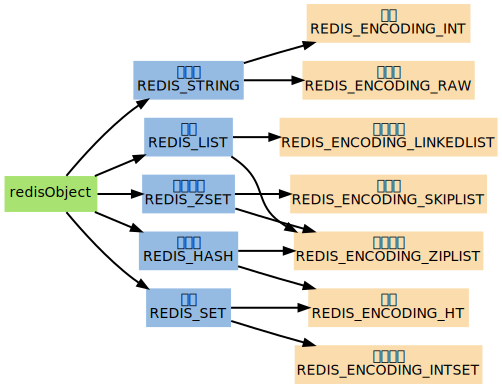
\includegraphics{graphviz-243b3a1747269b8e966a9bdd9db2129d983f2b23.pdf}

这个图展示了 Redis 各种数据类型,以及它们的编码方式。

\begin{notice}{note}{Note:}
\code{REDIS\_ENCODING\_ZIPMAP} 没有出现在图中,
因为从 Redis 2.6 开始,
它不再是任何数据类型的底层结构。
\end{notice}


\subsection{命令的类型检查和多态}
\label{datatype/object:id2}
有了 \code{redisObject} 结构的存在,
在执行处理数据类型的命令时,
进行类型检查和对编码进行多态操作就简单得多了。

当执行一个处理数据类型的命令时,
Redis 执行以下步骤:
\begin{enumerate}
\item {} 
根据给定 \code{key} ,在数据库字典中查找和它像对应的 \code{redisObject} ,如果没找到,就返回 \code{NULL} 。

\item {} 
检查 \code{redisObject} 的 \code{type} 属性和执行命令所需的类型是否相符,如果不相符,返回类型错误。

\item {} 
根据 \code{redisObject} 的 \code{encoding} 属性所指定的编码,选择合适的操作函数来处理底层的数据结构。

\item {} 
返回数据结构的操作结果作为命令的返回值。

\end{enumerate}

作为例子,以下展示了对键 \code{key} 执行 \code{LPOP} 命令的完整过程:

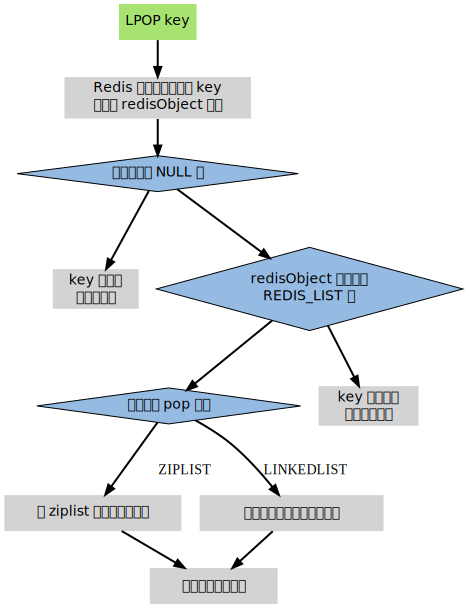
\includegraphics{graphviz-19bb826a6b2f1b39218ae00e804c65654128cc74.pdf}


\subsection{对象共享}
\label{datatype/object:id3}
有一些对象在 Redis 中非常常见,
比如命令的返回值 \code{OK} 、 \code{ERROR} 、 \code{WRONGTYPE} 等字符,
另外,一些小范围的整数,比如个位、十位、百位的整数都非常常见。

为了利用这种常见情况,
Redis 在内部使用了一个 \href{http://en.wikipedia.org/wiki/Flyweight\_pattern}{Flyweight 模式} :
通过预分配一些常见的值对象,
并在多个数据结构之间共享这些对象,
程序避免了重复分配的麻烦,
也节约了一些 CPU 时间。

Redis 预分配的值对象有如下这些:
\begin{itemize}
\item {} 
各种命令的返回值,比如执行成功时返回的 \code{OK} ,执行错误时返回的 \code{ERROR} ,类型错误时返回的 \code{WRONGTYPE} ,命令入队事务时返回的 \code{QUEUED} ,等等。

\item {} 
包括 \code{0} 在内,小于 \code{redis.h/REDIS\_SHARED\_INTEGERS} 的所有整数(\code{REDIS\_SHARED\_INTEGERS} 的默认值为 \code{10000})

\end{itemize}

因为命令的回复值直接返回给客户端,
所以它们的值无须进行共享;
另一方面,
如果某个命令的输入值是一个小于 \code{REDIS\_SHARED\_INTEGERS} 的整数对象,
那么当这个对象要被保存进数据库时,
Redis 就会释放原来的值,
并将值的指针指向共享对象。

作为例子,下图展示了三个列表,它们都带有指向共享对象数组中某个值对象的指针:

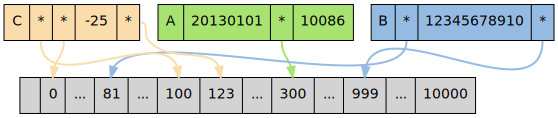
\includegraphics{graphviz-10fd6efbb50d4f8410ec42a39fa72d7247f90b4d.pdf}

三个列表的值分别为:
\begin{itemize}
\item {} 
列表 A : \code{{[}20130101, 300, 10086{]}} ,

\item {} 
列表 B : \code{{[}81, 12345678910, 999{]}} ,

\item {} 
列表 C : \code{{[}100, 0, -25, 123{]}} 。

\end{itemize}

\begin{notice}{note}{Note:}
共享对象只能被带指针的数据结构使用。

需要提醒的一点是,
共享对象只能被字典和双端链表这类能带有指针的数据结构使用。

像整数集合和压缩列表这些只能保存字符串、整数等字面值的内存数据结构,
就不能使用共享对象。
\end{notice}


\subsection{引用计数以及对象的销毁}
\label{datatype/object:id4}
当将 \code{redisObject} 用作数据库的键或者值,
而不是用来储存参数时,
对象的生命期是非常长的,
因为 C 语言本身没有自动释放内存的相关机制,
如果只依靠程序员的记忆来对对象进行追踪和销毁,
基本是不太可能的。

另一方面,正如前面提到的,一个共享对象可能被多个数据结构所引用,
这时像是“这个对象被引用了多少次?”之类的问题就会出现。

为了解决以上两个问题,
Redis 的对象系统使用了\href{http://en.wikipedia.org/wiki/Reference\_counting}{引用计数}技术来负责维持和销毁对象,
它的运作机制如下:
\begin{itemize}
\item {} 
每个 \code{redisObject} 结构都带有一个 \code{refcount} 属性,指示这个对象被引用了多少次。

\item {} 
当新创建一个对象时,它的 \code{refcount} 属性被设置为 \code{1} 。

\item {} 
当对一个对象进行共享时,Redis 将这个对象的 \code{refcount} 增一。

\item {} 
当使用完一个对象之后,或者取消对共享对象的引用之后,程序将对象的 \code{refcount} 减一。

\item {} 
当对象的 \code{refcount} 降至 \code{0} 时,这个 \code{redisObject} 结构,以及它所引用的数据结构的内存,都会被释放。

\end{itemize}


\subsection{小结}
\label{datatype/object:id6}\begin{itemize}
\item {} 
Redis 使用自己实现的对象机制来实现类型判断、命令多态和基于引用计数的垃圾回收。

\item {} 
一种 Redis 类型的键可以有多种底层实现。

\item {} 
Redis 会预分配一些常用的数据对象,并通过共享这些对象来减少内存占用,和避免频繁地为小对象分配内存。

\end{itemize}


\section{字符串}
\label{datatype/string::doc}\label{datatype/string:string-chapter}\label{datatype/string:id1}
\code{REDIS\_STRING} (字符串)是 Redis 使用得最为广泛的数据类型,
它除了是 \code{SET} 、 \code{GET} 等命令的操作对象之外,
数据库中的所有键,
以及执行命令时提供给 Redis 的参数,
都是用这种类型保存的。


\subsection{字符串编码}
\label{datatype/string:id2}
字符串类型分别使用 \code{REDIS\_ENCODING\_INT} 和 \code{REDIS\_ENCODING\_RAW} 两种编码:
\begin{itemize}
\item {} 
\code{REDIS\_ENCODING\_INT} 使用 \code{long} 类型来保存 \code{long} 类型值。

\item {} 
\code{REDIS\_ENCODING\_RAW} 则使用 \code{sdshdr} 结构来保存 \code{sds} (也即是 \code{char*} )、 \code{long long} 、 \code{double} 和 \code{long double} 类型值。

\end{itemize}

换句话来说,
在 Redis 中,
只有能表示为 \code{long} 类型的值,
才会以整数的形式保存,
其他类型的整数、小数和字符串,
都是用 \code{sdshdr} 结构来保存。

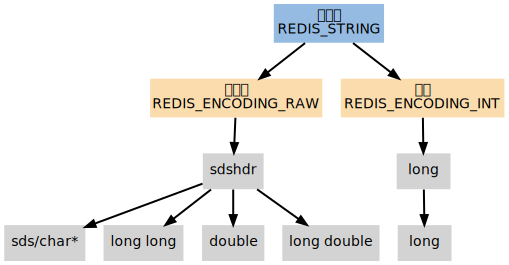
\includegraphics{graphviz-bb7ecaf3be8e729365b5a9241cdcb04aa5a709d1.pdf}


\subsection{编码的选择}
\label{datatype/string:id3}
新创建的字符串默认使用 \code{REDIS\_ENCODING\_RAW} 编码,
在将字符串作为键或者值保存进数据库时,
程序会尝试将字符串转为 \code{REDIS\_ENCODING\_INT} 编码。


\subsection{字符串命令的实现}
\label{datatype/string:id4}
Redis 的字符串类型命令,
基本上是通过包装 \code{sds} 数据结构的操作函数来实现的,
没有什么需要说明的地方。


\section{哈希表}
\label{datatype/hash:hash-chapter}\label{datatype/hash::doc}\label{datatype/hash:id1}
\code{REDIS\_HASH} (哈希表)是 \href{http://redis.readthedocs.org/en/latest/hash/hset.html\#hset}{\emph{HSET}} 、 \href{http://redis.readthedocs.org/en/latest/hash/hlen.html\#hlen}{\emph{HLEN}} 等命令的操作对象,
它使用 \code{REDIS\_ENCODING\_ZIPLIST} 和 \code{REDIS\_ENCODING\_HT} 两种编码方式:

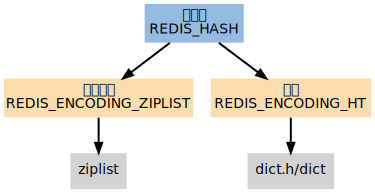
\includegraphics{graphviz-145365a458984496cfecacd67b29f5d42c39a401.pdf}


\subsection{字典编码的哈希表}
\label{datatype/hash:id2}
当哈希表使用字典编码时,
程序将哈希表的键(key)保存为字典的键,
将哈希表的值(value)保存为字典的值。

哈希表所使用的字典的键和值都是字符串对象。

下图展示了一个包含三个键值对的哈希表:

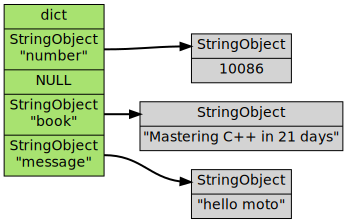
\includegraphics{graphviz-47d8c87484f68b0f34687f02b323dbd8d369d1ce.pdf}


\subsection{压缩列表编码的哈希表}
\label{datatype/hash:id3}
当使用 \code{REDIS\_ENCODING\_ZIPLIST} 编码哈希表时,
程序通过将键和值一同推入压缩列表,
从而形成保存哈希表所需的键-值对结构:

\begin{Verbatim}[commandchars=\\\{\}]
\PYG{o}{+}\PYG{o}{-}\PYG{o}{-}\PYG{o}{-}\PYG{o}{-}\PYG{o}{-}\PYG{o}{-}\PYG{o}{-}\PYG{o}{-}\PYG{o}{-}\PYG{o}{+}\PYG{o}{-}\PYG{o}{-}\PYG{o}{-}\PYG{o}{-}\PYG{o}{-}\PYG{o}{-}\PYG{o}{+}\PYG{o}{-}\PYG{o}{-}\PYG{o}{-}\PYG{o}{-}\PYG{o}{-}\PYG{o}{-}\PYG{o}{+}\PYG{o}{-}\PYG{o}{-}\PYG{o}{-}\PYG{o}{-}\PYG{o}{-}\PYG{o}{-}\PYG{o}{+}\PYG{o}{-}\PYG{o}{-}\PYG{o}{-}\PYG{o}{-}\PYG{o}{-}\PYG{o}{-}\PYG{o}{+}\PYG{o}{-}\PYG{o}{-}\PYG{o}{-}\PYG{o}{-}\PYG{o}{-}\PYG{o}{-}\PYG{o}{+}\PYG{o}{-}\PYG{o}{-}\PYG{o}{-}\PYG{o}{-}\PYG{o}{-}\PYG{o}{-}\PYG{o}{+}\PYG{o}{-}\PYG{o}{-}\PYG{o}{-}\PYG{o}{-}\PYG{o}{-}\PYG{o}{-}\PYG{o}{+}\PYG{o}{-}\PYG{o}{-}\PYG{o}{-}\PYG{o}{-}\PYG{o}{-}\PYG{o}{-}\PYG{o}{+}\PYG{o}{-}\PYG{o}{-}\PYG{o}{-}\PYG{o}{-}\PYG{o}{-}\PYG{o}{-}\PYG{o}{-}\PYG{o}{-}\PYG{o}{-}\PYG{o}{+}
\PYG{o}{\textbar{}} \PYG{n}{ZIPLIST} \PYG{o}{\textbar{}}      \PYG{o}{\textbar{}}      \PYG{o}{\textbar{}}      \PYG{o}{\textbar{}}      \PYG{o}{\textbar{}}      \PYG{o}{\textbar{}}      \PYG{o}{\textbar{}}      \PYG{o}{\textbar{}}      \PYG{o}{\textbar{}} \PYG{n}{ZIPLIST} \PYG{o}{\textbar{}}
\PYG{o}{\textbar{}} \PYG{n}{ENTRY}   \PYG{o}{\textbar{}} \PYG{n}{key1} \PYG{o}{\textbar{}} \PYG{n}{val1} \PYG{o}{\textbar{}} \PYG{n}{key2} \PYG{o}{\textbar{}} \PYG{n}{val2} \PYG{o}{\textbar{}} \PYG{p}{.}\PYG{p}{.}\PYG{p}{.}  \PYG{o}{\textbar{}} \PYG{p}{.}\PYG{p}{.}\PYG{p}{.}  \PYG{o}{\textbar{}} \PYG{n}{keyN} \PYG{o}{\textbar{}} \PYG{n}{valN} \PYG{o}{\textbar{}} \PYG{n}{ENTRY}   \PYG{o}{\textbar{}}
\PYG{o}{\textbar{}} \PYG{n}{HEAD}    \PYG{o}{\textbar{}}      \PYG{o}{\textbar{}}      \PYG{o}{\textbar{}}      \PYG{o}{\textbar{}}      \PYG{o}{\textbar{}}      \PYG{o}{\textbar{}}      \PYG{o}{\textbar{}}      \PYG{o}{\textbar{}}      \PYG{o}{\textbar{}} \PYG{n}{END}     \PYG{o}{\textbar{}}
\PYG{o}{+}\PYG{o}{-}\PYG{o}{-}\PYG{o}{-}\PYG{o}{-}\PYG{o}{-}\PYG{o}{-}\PYG{o}{-}\PYG{o}{-}\PYG{o}{-}\PYG{o}{+}\PYG{o}{-}\PYG{o}{-}\PYG{o}{-}\PYG{o}{-}\PYG{o}{-}\PYG{o}{-}\PYG{o}{+}\PYG{o}{-}\PYG{o}{-}\PYG{o}{-}\PYG{o}{-}\PYG{o}{-}\PYG{o}{-}\PYG{o}{+}\PYG{o}{-}\PYG{o}{-}\PYG{o}{-}\PYG{o}{-}\PYG{o}{-}\PYG{o}{-}\PYG{o}{+}\PYG{o}{-}\PYG{o}{-}\PYG{o}{-}\PYG{o}{-}\PYG{o}{-}\PYG{o}{-}\PYG{o}{+}\PYG{o}{-}\PYG{o}{-}\PYG{o}{-}\PYG{o}{-}\PYG{o}{-}\PYG{o}{-}\PYG{o}{+}\PYG{o}{-}\PYG{o}{-}\PYG{o}{-}\PYG{o}{-}\PYG{o}{-}\PYG{o}{-}\PYG{o}{+}\PYG{o}{-}\PYG{o}{-}\PYG{o}{-}\PYG{o}{-}\PYG{o}{-}\PYG{o}{-}\PYG{o}{+}\PYG{o}{-}\PYG{o}{-}\PYG{o}{-}\PYG{o}{-}\PYG{o}{-}\PYG{o}{-}\PYG{o}{+}\PYG{o}{-}\PYG{o}{-}\PYG{o}{-}\PYG{o}{-}\PYG{o}{-}\PYG{o}{-}\PYG{o}{-}\PYG{o}{-}\PYG{o}{-}\PYG{o}{+}
\end{Verbatim}

新添加的 key-value 对会被添加到压缩列表的表尾。

当进行查找/删除或更新操作时,程序先定位到键的位置,然后再通过对键的位置来定位值的位置。


\subsection{编码的选择}
\label{datatype/hash:id4}
创建空白哈希表时,
程序默认使用 \code{REDIS\_ENCODING\_ZIPLIST} 编码,
当以下任何一个条件被满足时,
程序将编码从切换为 \code{REDIS\_ENCODING\_HT} :
\begin{itemize}
\item {} 
哈希表中某个键或某个值的长度大于 \code{server.hash\_max\_ziplist\_value} (默认值为 \code{64} )。

\item {} 
压缩列表中的节点数量大于 \code{server.hash\_max\_ziplist\_entries} (默认值为 \code{512} )。

\end{itemize}


\subsection{哈希命令的实现}
\label{datatype/hash:id5}
哈希类型命令的实现全都是对字典和压缩列表操作函数的包装,
以及几个在两种编码之间进行转换的函数,
没有特别要讲解的地方。


\section{列表}
\label{datatype/list:list-chapter}\label{datatype/list::doc}\label{datatype/list:id1}
\code{REDIS\_LIST} (列表)是 \href{http://redis.readthedocs.org/en/latest/list/lpush.html\#lpush}{\emph{LPUSH}} 、 \href{http://redis.readthedocs.org/en/latest/list/lrange.html\#lrange}{\emph{LRANGE}} 等命令的操作对象,
它使用 \code{REDIS\_ENCODING\_ZIPLIST} 和 \code{REDIS\_ENCODING\_LINKEDLIST} 这两种方式编码:

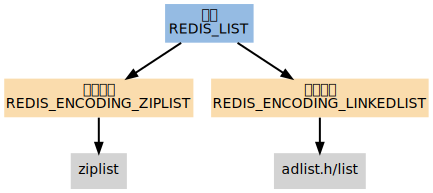
\includegraphics{graphviz-9d1b937227cf948b8a9bfb3137570475e5407d2c.pdf}


\subsection{编码的选择}
\label{datatype/list:id2}
创建新列表时 Redis 默认使用 \code{REDIS\_ENCODING\_ZIPLIST} 编码,
当以下任意一个条件被满足时,
列表会被转换成 \code{REDIS\_ENCODING\_LINKEDLIST} 编码:
\begin{itemize}
\item {} 
试图往列表新添加一个字符串值,且这个字符串的长度超过 \code{server.list\_max\_ziplist\_value} (默认值为 \code{64} )。

\item {} 
\code{ziplist} 包含的节点超过 \code{server.list\_max\_ziplist\_entries} (默认值为 \code{512} )。

\end{itemize}


\subsection{列表命令的实现}
\label{datatype/list:id3}
因为两种底层实现的抽象方式和列表的抽象方式非常接近,
所以列表命令几乎就是通过一对一地映射到底层数据结构的操作来实现的。

既然这些映射都非常直观,
这里就不做赘述了,
在以下的内容中,
我们将焦点放在 \href{http://redis.readthedocs.org/en/latest/list/blpop.html\#blpop}{\emph{BLPOP}} 、 \href{http://redis.readthedocs.org/en/latest/list/brpop.html\#brpop}{\emph{BRPOP}} 和 \href{http://redis.readthedocs.org/en/latest/list/brpoplpush.html\#brpoplpush}{\emph{BRPOPLPUSH}} 这个几个阻塞命令的实现原理上。


\subsection{阻塞的条件}
\label{datatype/list:id4}
\href{http://redis.readthedocs.org/en/latest/list/blpop.html\#blpop}{\emph{BLPOP}} 、 \href{http://redis.readthedocs.org/en/latest/list/brpop.html\#brpop}{\emph{BRPOP}} 和 \href{http://redis.readthedocs.org/en/latest/list/brpoplpush.html\#brpoplpush}{\emph{BRPOPLPUSH}} 三个命令都可能造成客户端被阻塞,
以下将这些命令统称为列表的阻塞原语。

阻塞原语并不是一定会造成客户端阻塞:
\begin{itemize}
\item {} 
只有当这些命令被用于空列表时, 它们才会阻塞客户端。

\item {} 
如果被处理的列表不为空的话, 它们就执行无阻塞版本的 \href{http://redis.readthedocs.org/en/latest/list/lpop.html\#lpop}{\emph{LPOP}} 、 \href{http://redis.readthedocs.org/en/latest/list/rpop.html\#rpop}{\emph{RPOP}} 或 \href{http://redis.readthedocs.org/en/latest/list/rpoplpush.html\#rpoplpush}{\emph{RPOPLPUSH}} 命令。

\end{itemize}

作为例子,以下流程图展示了 \href{http://redis.readthedocs.org/en/latest/list/blpop.html\#blpop}{\emph{BLPOP}} 决定是否对客户端进行阻塞过程:

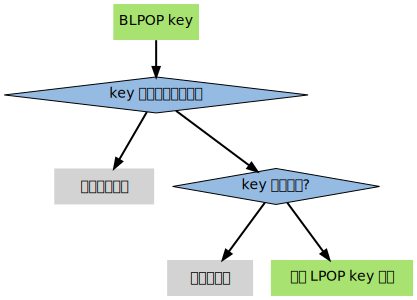
\includegraphics{graphviz-657d8e78e1f1357fdff05173a259334670b87f85.pdf}


\subsection{阻塞}
\label{datatype/list:id5}
当一个阻塞原语的处理目标为空键时,
执行该阻塞原语的客户端就会被阻塞。

阻塞一个客户端需要执行以下步骤:
\begin{enumerate}
\item {} 
将客户端的状态设为“正在阻塞”,并记录阻塞这个客户端的各个键,以及阻塞的最长时限(timeout)等数据。

\item {} 
将客户端的信息记录到 \code{server.db{[}i{]}-\textgreater{}blocking\_keys} 中(其中 \code{i} 为客户端所使用的数据库号码)。

\item {} 
继续维持客户端和服务器之间的网络连接,但不再向客户端传送任何信息,造成客户端阻塞。

\end{enumerate}

步骤 2 是将来解除阻塞的关键,
\code{server.db{[}i{]}-\textgreater{}blocking\_keys} 是一个字典,
字典的键是那些造成客户端阻塞的键,
而字典的值是一个链表,
链表里保存了所有因为这个键而被阻塞的客户端
(被同一个键所阻塞的客户端可能不止一个):

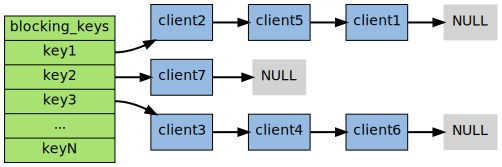
\includegraphics{graphviz-72233dd6a912518ff6874fdad4e20356091a6063.pdf}

在上图展示的 \code{blocking\_keys} 例子中, \code{client2} 、 \code{client5} 和 \code{client1} 三个客户端就正被 \code{key1} 阻塞,
而其他几个客户端也正在被别的两个 key 阻塞。

当客户端被阻塞之后,脱离阻塞状态有以下三种方法:
\begin{enumerate}
\item {} 
被动脱离:有其他客户端为造成阻塞的键推入了新元素。

\item {} 
主动脱离:到达执行阻塞原语时设定的最大阻塞时间。

\item {} 
强制脱离:客户端强制终止和服务器的连接,或者服务器停机。

\end{enumerate}

以下内容将分别介绍被动脱离和主动脱离的实现方式。


\subsection{阻塞因 LPUSH 、 RPUSH 、 LINSERT 等添加命令而被取消}
\label{datatype/list:lpush-rpush-linsert}
通过将新元素推入造成客户端阻塞的某个键中,
可以让相应的客户端从阻塞状态中脱离出来
(取消阻塞的客户端数量取决于推入元素的数量)。

\href{http://redis.readthedocs.org/en/latest/list/lpush.html\#lpush}{\emph{LPUSH}} 、 \href{http://redis.readthedocs.org/en/latest/list/rpush.html\#rpush}{\emph{RPUSH}} 和 \href{http://redis.readthedocs.org/en/latest/list/linsert.html\#linsert}{\emph{LINSERT}} 这三个添加新元素到列表的命令,
在底层都由一个 \code{pushGenericCommand} 的函数实现,
这个函数的运作流程如下图:

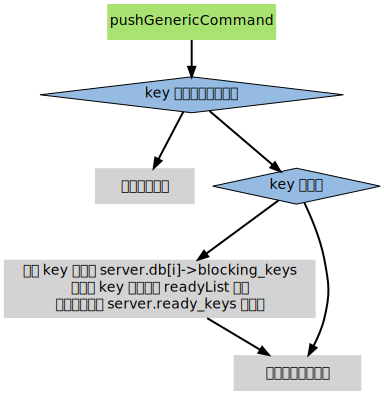
\includegraphics{graphviz-be4975476661a3e683475377d30b659d70bee64c.pdf}

当向一个空键推入新元素时,
\code{pushGenericCommand} 函数执行以下两件事:
\begin{enumerate}
\item {} 
检查这个键是否存在于前面提到的 \code{server.db{[}i{]}-\textgreater{}blocking\_keys} 字典里, 如果是的话, 那么说明有至少一个客户端因为这个 key 而被阻塞,程序会为这个键创建一个 \code{redis.h/readyList} 结构, 并将它添加到 \code{server.ready\_keys} 链表中。

\item {} 
将给定的值添加到列表键中。

\end{enumerate}

\code{readyList} 结构的定义如下:

\begin{Verbatim}[commandchars=\\\{\}]
\PYG{k}{typedef} \PYG{k}{struct} \PYG{n}{readyList} \PYG{p}{\PYGZob{}}
    \PYG{n}{redisDb} \PYG{o}{*}\PYG{n}{db}\PYG{p}{;}
    \PYG{n}{robj} \PYG{o}{*}\PYG{n}{key}\PYG{p}{;}
\PYG{p}{\PYGZcb{}} \PYG{n}{readyList}\PYG{p}{;}
\end{Verbatim}

\code{readyList} 结构的 \code{key} 属性指向造成阻塞的键,而 \code{db} 则指向该键所在的数据库。

举个例子,
假设某个非阻塞客户端正在使用 \code{0} 号数据库,
而这个数据库当前的 \code{blocking\_keys} 属性的值如下:

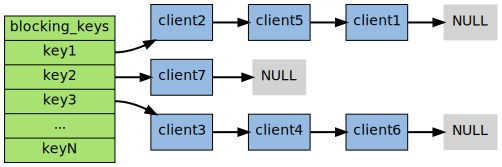
\includegraphics{graphviz-72233dd6a912518ff6874fdad4e20356091a6063.pdf}

如果这时客户端对该数据库执行 \code{PUSH key3 value} ,
那么 \code{pushGenericCommand} 将创建一个 \code{db} 属性指向 \code{0} 号数据库、
\code{key} 属性指向 \code{key3} 键对象的 \code{readyList} 结构 ,
并将它添加到服务器 \code{server.ready\_keys} 属性的链表中:

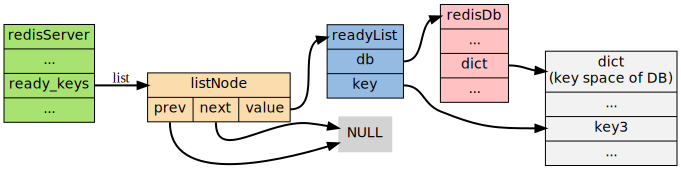
\includegraphics{graphviz-f2450c693b205a3c1cf1e82a4a09150c614ed631.pdf}

在我们这个例子中,
到目前为止,
\code{pushGenericCommand} 函数完成了以下两件事:
\begin{enumerate}
\item {} 
将 \code{readyList} 添加到服务器。

\item {} 
将新元素 \code{value} 添加到键 \code{key3} 。

\end{enumerate}

虽然 \code{key3} 已经不再是空键,
但到目前为止,
被 \code{key3} 阻塞的客户端还没有任何一个被解除阻塞状态。

为了做到这一点,
Redis 的主进程在执行完 \code{pushGenericCommand} 函数之后,
会继续调用 \code{handleClientsBlockedOnLists} 函数,
这个函数执行以下操作:
\begin{enumerate}
\item {} 
如果 \code{server.ready\_keys} 不为空,那么弹出该链表的表头元素,并取出元素中的 \code{readyList} 值。

\item {} 
根据 \code{readyList} 值所保存的 \code{key} 和 \code{db} ,在 \code{server.blocking\_keys} 中查找所有因为 \code{key} 而被阻塞的客户端(以链表的形式保存)。

\item {} 
如果 \code{key} 不为空,那么从 \code{key} 中弹出一个元素,并弹出客户端链表的第一个客户端,然后将被弹出元素返回给被弹出客户端作为阻塞原语的返回值。

\item {} 
根据 \code{readyList} 结构的属性,删除 \code{server.blocking\_keys} 中相应的客户端数据,取消客户端的阻塞状态。

\item {} 
继续执行步骤 3 和 4 ,直到 \code{key} 没有元素可弹出,或者所有因为 \code{key} 而阻塞的客户端都取消阻塞为止。

\item {} 
继续执行步骤 1 ,直到 \code{ready\_keys} 链表里的所有 \code{readyList} 结构都被处理完为止。

\end{enumerate}

用一段伪代码描述以上操作可能会更直观一些:

\begin{Verbatim}[commandchars=\\\{\}]
\PYG{k}{def} \PYG{n+nf}{handleClientsBlockedOnLists}\PYG{p}{(}\PYG{p}{)}\PYG{p}{:}

    \PYG{c}{\PYGZsh{} 执行直到 ready\PYGZus{}keys 为空}
    \PYG{k}{while} \PYG{n}{server}\PYG{o}{.}\PYG{n}{ready\PYGZus{}keys} \PYG{o}{!=} \PYG{n}{NULL}\PYG{p}{:}

        \PYG{c}{\PYGZsh{} 弹出链表中的第一个 readyList}
        \PYG{n}{rl} \PYG{o}{=} \PYG{n}{server}\PYG{o}{.}\PYG{n}{ready\PYGZus{}keys}\PYG{o}{.}\PYG{n}{pop\PYGZus{}first\PYGZus{}node}\PYG{p}{(}\PYG{p}{)}

        \PYG{c}{\PYGZsh{} 遍历所有因为这个键而被阻塞的客户端}
        \PYG{k}{for} \PYG{n}{client} \PYG{o+ow}{in} \PYG{n}{all\PYGZus{}client\PYGZus{}blocking\PYGZus{}by\PYGZus{}key}\PYG{p}{(}\PYG{n}{rl}\PYG{o}{.}\PYG{n}{key}\PYG{p}{,} \PYG{n}{rl}\PYG{o}{.}\PYG{n}{db}\PYG{p}{)}\PYG{p}{:}

            \PYG{c}{\PYGZsh{} 只要还有客户端被这个键阻塞,就一直从键中弹出元素}
            \PYG{c}{\PYGZsh{} 如果被阻塞客户端执行的是 BLPOP ,那么对键执行 LPOP}
            \PYG{c}{\PYGZsh{} 如果执行的是 BRPOP ,那么对键执行 RPOP}
            \PYG{n}{element} \PYG{o}{=} \PYG{n}{rl}\PYG{o}{.}\PYG{n}{key}\PYG{o}{.}\PYG{n}{pop\PYGZus{}element}\PYG{p}{(}\PYG{p}{)}

            \PYG{k}{if} \PYG{n}{element} \PYG{o}{==} \PYG{n}{NULL}\PYG{p}{:}
                \PYG{c}{\PYGZsh{} 键为空,跳出 for 循环}
                \PYG{c}{\PYGZsh{} 余下的未解除阻塞的客户端只能等待下次新元素的进入了}
                \PYG{k}{break}
            \PYG{k}{else}\PYG{p}{:}
                \PYG{c}{\PYGZsh{} 清除客户端的阻塞信息}
                \PYG{n}{server}\PYG{o}{.}\PYG{n}{blocking\PYGZus{}keys}\PYG{o}{.}\PYG{n}{remove\PYGZus{}blocking\PYGZus{}info}\PYG{p}{(}\PYG{n}{client}\PYG{p}{)}
                \PYG{c}{\PYGZsh{} 将元素返回给客户端,脱离阻塞状态}
                \PYG{n}{client}\PYG{o}{.}\PYG{n}{reply\PYGZus{}list\PYGZus{}item}\PYG{p}{(}\PYG{n}{element}\PYG{p}{)}
\end{Verbatim}


\subsection{先阻塞先服务(FBFS)策略}
\label{datatype/list:fbfs}
值得一提的是,
当程序添加一个新的被阻塞客户端到 \code{server.blocking\_keys} 字典的链表中时,
它将该客户端放在链表的最后,
而当 \code{handleClientsBlockedOnLists} 取消客户端的阻塞时,
它从链表的最前面开始取消阻塞:
这个链表形成了一个 FIFO 队列,
最先被阻塞的客户端总值最先脱离阻塞状态,
Redis 文档称这种模式为先阻塞先服务(FBFS,first-block-first-serve)。

举个例子,在下图所示的阻塞状况中,
如果客户端对数据库执行 \code{PUSH key3 value} ,
那么只有 \code{client3} 会被取消阻塞,
\code{client6} 和 \code{client4} 仍然阻塞;
如果客户端对数据库执行 \code{PUSH key3 value1 value2} ,
那么 \code{client3} 和 \code{client4} 的阻塞都会被取消,
而客户端 \code{client6} 依然处于阻塞状态:

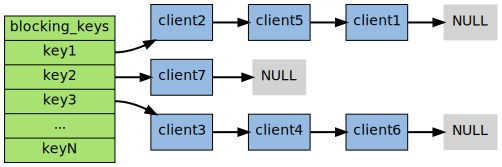
\includegraphics{graphviz-72233dd6a912518ff6874fdad4e20356091a6063.pdf}


\subsection{阻塞因超过最大等待时间而被取消}
\label{datatype/list:id6}
前面提到过,
当客户端被阻塞时,
所有造成它阻塞的键,
以及阻塞的最长时限会被记录在客户端里面,
并且该客户端的状态会被设置为“正在阻塞”。

每次 Redis 服务器常规操作函数(server cron job)执行时,
程序都会检查所有连接到服务器的客户端,
查看那些处于“正在阻塞”状态的客户端的最大阻塞时限是否已经过期,
如果是的话,
就给客户端返回一个空白回复,
然后撤销对客户端的阻塞。

可以用一段伪代码来描述这个过程:

\begin{Verbatim}[commandchars=\\\{\}]
\PYG{k}{def} \PYG{n+nf}{server\PYGZus{}cron\PYGZus{}job}\PYG{p}{(}\PYG{p}{)}\PYG{p}{:}

    \PYG{c}{\PYGZsh{} 其他操作 ...}

    \PYG{c}{\PYGZsh{} 遍历所有已连接客户端}
    \PYG{k}{for} \PYG{n}{client} \PYG{o+ow}{in} \PYG{n}{server}\PYG{o}{.}\PYG{n}{all\PYGZus{}connected\PYGZus{}client}\PYG{p}{:}

        \PYG{c}{\PYGZsh{} 如果客户端状态为“正在阻塞”,并且最大阻塞时限已到达}
        \PYG{k}{if} \PYG{n}{client}\PYG{o}{.}\PYG{n}{state} \PYG{o}{==} \PYG{n}{BLOCKING} \PYG{o+ow}{and} \PYGZbs{}
           \PYG{n}{client}\PYG{o}{.}\PYG{n}{max\PYGZus{}blocking\PYGZus{}timestamp} \PYG{o}{\PYGZlt{}} \PYG{n}{current\PYGZus{}timestamp}\PYG{p}{(}\PYG{p}{)}\PYG{p}{:}

            \PYG{c}{\PYGZsh{} 那么给客户端发送空回复,脱离阻塞状态}
            \PYG{n}{client}\PYG{o}{.}\PYG{n}{send\PYGZus{}empty\PYGZus{}reply}\PYG{p}{(}\PYG{p}{)}

            \PYG{c}{\PYGZsh{} 并清除客户端在服务器上的阻塞信息}
            \PYG{n}{server}\PYG{o}{.}\PYG{n}{blocking\PYGZus{}keys}\PYG{o}{.}\PYG{n}{remove\PYGZus{}blocking\PYGZus{}info}\PYG{p}{(}\PYG{n}{client}\PYG{p}{)}

    \PYG{c}{\PYGZsh{} 其他操作 ...}
\end{Verbatim}


\section{集合}
\label{datatype/set:set-chapter}\label{datatype/set::doc}\label{datatype/set:id1}
\code{REDIS\_SET} (集合)是 \href{http://redis.readthedocs.org/en/latest/set/sadd.html\#sadd}{\emph{SADD}} 、 \href{http://redis.readthedocs.org/en/latest/set/srandmember.html\#srandmember}{\emph{SRANDMEMBER}} 等命令的操作对象,
它使用 \code{REDIS\_ENCODING\_INTSET} 和 \code{REDIS\_ENCODING\_HT} 两种方式编码:

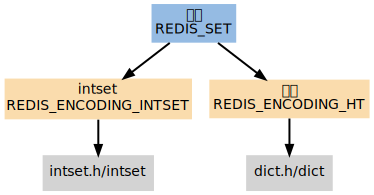
\includegraphics{graphviz-2f54a5b62b3507f0e6d579358e426c78b0dfbd5c.pdf}


\subsection{编码的选择}
\label{datatype/set:id2}
第一个添加到集合的元素,
决定了创建集合时所使用的编码:
\begin{itemize}
\item {} 
如果第一个元素可以表示为 \code{long long} 类型值(也即是,它是一个整数), 那么集合的初始编码为 \code{REDIS\_ENCODING\_INTSET} 。

\item {} 
否则,集合的初始编码为 \code{REDIS\_ENCODING\_HT} 。

\end{itemize}


\subsection{编码的切换}
\label{datatype/set:id3}
如果一个集合使用 \code{REDIS\_ENCODING\_INTSET} 编码,
那么当以下任何一个条件被满足时,
这个集合会被转换成 \code{REDIS\_ENCODING\_HT} 编码:
\begin{itemize}
\item {} 
\code{intset} 保存的整数值个数超过 \code{server.set\_max\_intset\_entries} (默认值为 \code{512} )。

\item {} 
试图往集合里添加一个新元素,并且这个元素不能被表示为 \code{long long} 类型(也即是,它不是一个整数)。

\end{itemize}


\subsection{字典编码的集合}
\label{datatype/set:id4}
当使用 \code{REDIS\_ENCODING\_HT} 编码时,
集合将元素保存到字典的键里面,
而字典的值则统一设为 \code{NULL} 。

作为例子,
以下图片展示了一个以 \code{REDIS\_ENCODING\_HT} 编码表示的集合,
集合的成员为 \code{elem1} 、 \code{elem2} 和 \code{elem3} :

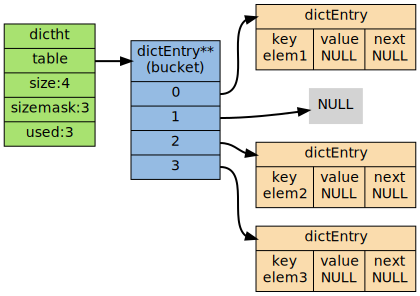
\includegraphics{graphviz-3b62c50ed475dc6c91adbb8079f0e0104f644931.pdf}


\subsection{集合命令的实现}
\label{datatype/set:id5}
Redis 集合类型命令的实现,
主要是对 \code{intset} 和 \code{dict} 两个数据结构的操作函数的包装,
以及一些在两种编码之间进行转换的函数,
大部分都没有什么需要解释的地方,
唯一比较有趣的是 \href{http://redis.readthedocs.org/en/latest/set/sinter.html\#sinter}{\emph{SINTER}} 、 \href{http://redis.readthedocs.org/en/latest/set/sunion.html\#sunion}{\emph{SUNION}} 等命令之下的算法实现,
以下三个小节就分别讨论它们所使用的算法。


\subsection{求交集算法}
\label{datatype/set:id6}
\href{http://redis.readthedocs.org/en/latest/set/sinter.html\#sinter}{\emph{SINTER}} 和 \href{http://redis.readthedocs.org/en/latest/set/sinterstore.html\#sinterstore}{\emph{SINTERSTORE}} 两个命令所使用的求并交集算法可以用 Python 表示如下:

\begin{Verbatim}[commandchars=\\\{\}]
\PYG{c}{\PYGZsh{} coding: utf-8}

\PYG{k}{def} \PYG{n+nf}{sinter}\PYG{p}{(}\PYG{o}{*}\PYG{n}{multi\PYGZus{}set}\PYG{p}{)}\PYG{p}{:}

    \PYG{c}{\PYGZsh{} 根据集合的基数进行排序}
    \PYG{n}{sorted\PYGZus{}multi\PYGZus{}set} \PYG{o}{=} \PYG{n+nb}{sorted}\PYG{p}{(}\PYG{n}{multi\PYGZus{}set}\PYG{p}{,} \PYG{k}{lambda} \PYG{n}{x}\PYG{p}{,} \PYG{n}{y}\PYG{p}{:} \PYG{n+nb}{len}\PYG{p}{(}\PYG{n}{x}\PYG{p}{)} \PYG{o}{-} \PYG{n+nb}{len}\PYG{p}{(}\PYG{n}{y}\PYG{p}{)}\PYG{p}{)}

    \PYG{c}{\PYGZsh{} 使用基数最小的集合作为基础结果集,有助于降低常数项}
    \PYG{n}{result} \PYG{o}{=} \PYG{n}{sorted\PYGZus{}multi\PYGZus{}set}\PYG{p}{[}\PYG{l+m+mi}{0}\PYG{p}{]}\PYG{o}{.}\PYG{n}{copy}\PYG{p}{(}\PYG{p}{)}

    \PYG{c}{\PYGZsh{} 剔除所有在 sorted\PYGZus{}multi\PYGZus{}set[0] 中存在}
    \PYG{c}{\PYGZsh{} 但在其他某个集合中不存在的元素}
    \PYG{k}{for} \PYG{n}{elem} \PYG{o+ow}{in} \PYG{n}{sorted\PYGZus{}multi\PYGZus{}set}\PYG{p}{[}\PYG{l+m+mi}{0}\PYG{p}{]}\PYG{p}{:}

        \PYG{k}{for} \PYG{n}{s} \PYG{o+ow}{in} \PYG{n}{sorted\PYGZus{}multi\PYGZus{}set}\PYG{p}{[}\PYG{l+m+mi}{1}\PYG{p}{:}\PYG{p}{]}\PYG{p}{:}

            \PYG{k}{if} \PYG{p}{(}\PYG{o+ow}{not} \PYG{n}{elem} \PYG{o+ow}{in} \PYG{n}{s}\PYG{p}{)}\PYG{p}{:}
                \PYG{n}{result}\PYG{o}{.}\PYG{n}{remove}\PYG{p}{(}\PYG{n}{elem}\PYG{p}{)}
                \PYG{k}{break}

    \PYG{k}{return} \PYG{n}{result}
\end{Verbatim}

算法的复杂度为 $O(N^2)$ ,
执行步数为 $S * T$ ,
其中 $S$ 为输入集合中基数最小的集合,
而 $T$ 则为输入集合的数量。


\subsection{求并集算法}
\label{datatype/set:id7}
\href{http://redis.readthedocs.org/en/latest/set/sunion.html\#sunion}{\emph{SUNION}} 和 \href{http://redis.readthedocs.org/en/latest/set/sunionstore.html\#sunionstore}{\emph{SUNIONSTORE}} 两个命令所使用的求并集算法可以用 Python 表示如下:

\begin{Verbatim}[commandchars=\\\{\}]
\PYG{c}{\PYGZsh{} coding: utf-8}

\PYG{k}{def} \PYG{n+nf}{sunion}\PYG{p}{(}\PYG{o}{*}\PYG{n}{multi\PYGZus{}set}\PYG{p}{)}\PYG{p}{:}

    \PYG{n}{result} \PYG{o}{=} \PYG{n+nb}{set}\PYG{p}{(}\PYG{p}{)}

    \PYG{k}{for} \PYG{n}{s} \PYG{o+ow}{in} \PYG{n}{multi\PYGZus{}set}\PYG{p}{:}
        \PYG{k}{for} \PYG{n}{elem} \PYG{o+ow}{in} \PYG{n}{s}\PYG{p}{:}
            \PYG{c}{\PYGZsh{} 重复的元素会被自动忽略}
            \PYG{n}{result}\PYG{o}{.}\PYG{n}{add}\PYG{p}{(}\PYG{n}{elem}\PYG{p}{)}

    \PYG{k}{return} \PYG{n}{result}
\end{Verbatim}

算法的复杂度为 $O(N)$ 。


\subsection{求差集算法}
\label{datatype/set:id8}
Redis 为 \href{http://redis.readthedocs.org/en/latest/set/sdiff.html\#sdiff}{\emph{SDIFF}} 和 \href{http://redis.readthedocs.org/en/latest/set/sdiffstore.html\#sdiffstore}{\emph{SDIFFSTORE}} 两个命令准备了两种求集合差的算法。

以 Python 代码表示的算法一定义如下:

\begin{Verbatim}[commandchars=\\\{\}]
\PYG{c}{\PYGZsh{} coding: utf-8}

\PYG{k}{def} \PYG{n+nf}{sdiff\PYGZus{}1}\PYG{p}{(}\PYG{o}{*}\PYG{n}{multi\PYGZus{}set}\PYG{p}{)}\PYG{p}{:}

    \PYG{n}{result} \PYG{o}{=} \PYG{n}{multi\PYGZus{}set}\PYG{p}{[}\PYG{l+m+mi}{0}\PYG{p}{]}\PYG{o}{.}\PYG{n}{copy}\PYG{p}{(}\PYG{p}{)}

    \PYG{n}{sorted\PYGZus{}multi\PYGZus{}set} \PYG{o}{=} \PYG{n+nb}{sorted}\PYG{p}{(}\PYG{n}{multi\PYGZus{}set}\PYG{p}{[}\PYG{l+m+mi}{1}\PYG{p}{:}\PYG{p}{]}\PYG{p}{,} \PYG{k}{lambda} \PYG{n}{x}\PYG{p}{,} \PYG{n}{y}\PYG{p}{:} \PYG{n+nb}{len}\PYG{p}{(}\PYG{n}{x}\PYG{p}{)} \PYG{o}{-} \PYG{n+nb}{len}\PYG{p}{(}\PYG{n}{y}\PYG{p}{)}\PYG{p}{)}

    \PYG{c}{\PYGZsh{} 当 elem 存在于除 multi\PYGZus{}set[0] 之外的集合时}
    \PYG{c}{\PYGZsh{} 将 elem 从 result 中删除}
    \PYG{k}{for} \PYG{n}{elem} \PYG{o+ow}{in} \PYG{n}{multi\PYGZus{}set}\PYG{p}{[}\PYG{l+m+mi}{0}\PYG{p}{]}\PYG{p}{:}

        \PYG{k}{for} \PYG{n}{s} \PYG{o+ow}{in} \PYG{n}{sorted\PYGZus{}multi\PYGZus{}set}\PYG{p}{:}

            \PYG{k}{if} \PYG{n}{elem} \PYG{o+ow}{in} \PYG{n}{s}\PYG{p}{:}
                \PYG{n}{result}\PYG{o}{.}\PYG{n}{remove}\PYG{p}{(}\PYG{n}{elem}\PYG{p}{)}
                \PYG{k}{break}

    \PYG{k}{return} \PYG{n}{result}
\end{Verbatim}

这个算法的复杂度为 $O(N^2)$ ,
执行步数为 $S*T$ ,
其中 $S$ 为输入集合中基数最小的集合,
而 $T$ 则为除第一个集合之外,
其他集合的数量。

以 Python 代码表示的算法二定于如下:

\begin{Verbatim}[commandchars=\\\{\}]
\PYG{c}{\PYGZsh{} coding: utf-8}

\PYG{k}{def} \PYG{n+nf}{sdiff\PYGZus{}2}\PYG{p}{(}\PYG{o}{*}\PYG{n}{multi\PYGZus{}set}\PYG{p}{)}\PYG{p}{:}
    \PYG{c}{\PYGZsh{} 用第一个集合作为结果集的起始值}
    \PYG{n}{result} \PYG{o}{=} \PYG{n}{multi\PYGZus{}set}\PYG{p}{[}\PYG{l+m+mi}{0}\PYG{p}{]}\PYG{o}{.}\PYG{n}{copy}\PYG{p}{(}\PYG{p}{)}

    \PYG{k}{for} \PYG{n}{s} \PYG{o+ow}{in} \PYG{n}{multi\PYGZus{}set}\PYG{p}{[}\PYG{l+m+mi}{1}\PYG{p}{:}\PYG{p}{]}\PYG{p}{:}
        \PYG{k}{for} \PYG{n}{elem} \PYG{o+ow}{in} \PYG{n}{s}\PYG{p}{:}
            \PYG{c}{\PYGZsh{} 从结果集中删去其他集合中包含的元素}
            \PYG{k}{if} \PYG{n}{elem} \PYG{o+ow}{in} \PYG{n}{result}\PYG{p}{:}
                \PYG{n}{result}\PYG{o}{.}\PYG{n}{remove}\PYG{p}{(}\PYG{n}{elem}\PYG{p}{)}

    \PYG{k}{return} \PYG{n}{result}
\end{Verbatim}

这个算法的复杂度同样为 $O(N^2)$ ,
执行步数为 $S$ ,
其中 $S$ 为所有集合的基数总和。

Redis 使用一个程序决定该使用那个求差集算法,
程序用 Python 表示如下:

\begin{Verbatim}[commandchars=\\\{\}]
\PYG{c}{\PYGZsh{} coding: utf-8}

\PYG{k+kn}{from} \PYG{n+nn}{sdiff\PYGZus{}1} \PYG{k+kn}{import} \PYG{n}{sdiff\PYGZus{}1}
\PYG{k+kn}{from} \PYG{n+nn}{sdiff\PYGZus{}2} \PYG{k+kn}{import} \PYG{n}{sdiff\PYGZus{}2}

\PYG{k}{def} \PYG{n+nf}{sdiff}\PYG{p}{(}\PYG{o}{*}\PYG{n}{multi\PYGZus{}set}\PYG{p}{)}\PYG{p}{:}

    \PYG{c}{\PYGZsh{} 算法一的常数项较低,给它一点额外的优先级}
    \PYG{n}{algo\PYGZus{}one\PYGZus{}advantage} \PYG{o}{=} \PYG{l+m+mi}{2} 
    \PYG{n}{algo\PYGZus{}one\PYGZus{}weight} \PYG{o}{=} \PYG{n+nb}{len}\PYG{p}{(}\PYG{n}{multi\PYGZus{}set}\PYG{p}{[}\PYG{l+m+mi}{0}\PYG{p}{]}\PYG{p}{)} \PYG{o}{*} \PYG{n+nb}{len}\PYG{p}{(}\PYG{n}{multi\PYGZus{}set}\PYG{p}{[}\PYG{l+m+mi}{1}\PYG{p}{:}\PYG{p}{]}\PYG{p}{)} \PYG{o}{/} \PYG{n}{algo\PYGZus{}one\PYGZus{}advantage}

    \PYG{n}{algo\PYGZus{}two\PYGZus{}weight} \PYG{o}{=} \PYG{n+nb}{sum}\PYG{p}{(}\PYG{n+nb}{map}\PYG{p}{(}\PYG{n+nb}{len}\PYG{p}{,} \PYG{n}{multi\PYGZus{}set}\PYG{p}{)}\PYG{p}{)}

    \PYG{k}{if} \PYG{n}{algo\PYGZus{}one\PYGZus{}weight} \PYG{o}{\PYGZlt{}}\PYG{o}{=} \PYG{n}{algo\PYGZus{}two\PYGZus{}weight}\PYG{p}{:}
        \PYG{k}{return} \PYG{n}{sdiff\PYGZus{}1}\PYG{p}{(}\PYG{o}{*}\PYG{n}{multi\PYGZus{}set}\PYG{p}{)}
    \PYG{k}{else}\PYG{p}{:}
        \PYG{k}{return} \PYG{n}{sdiff\PYGZus{}2}\PYG{p}{(}\PYG{o}{*}\PYG{n}{multi\PYGZus{}set}\PYG{p}{)}
\end{Verbatim}


\section{有序集}
\label{datatype/sorted_set:sorted-set-chapter}\label{datatype/sorted_set::doc}\label{datatype/sorted_set:id1}
\code{REDIS\_ZSET} (有序集)是 \href{http://redis.readthedocs.org/en/latest/sorted\_set/zadd.html\#zadd}{\emph{ZADD}} 、 \href{http://redis.readthedocs.org/en/latest/sorted\_set/zcount.html\#zcount}{\emph{ZCOUNT}} 等命令的操作对象,
它使用 \code{REDIS\_ENCODING\_ZIPLIST} 和 \code{REDIS\_ENCODING\_SKIPLIST} 两种方式编码:

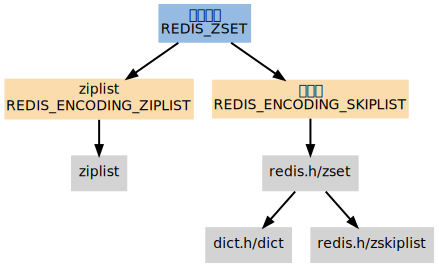
\includegraphics{graphviz-4d10098056ec25ed0e239f64bbcac524bce31bc8.pdf}


\subsection{编码的选择}
\label{datatype/sorted_set:id2}
在通过 \href{http://redis.readthedocs.org/en/latest/sorted\_set/zadd.html\#zadd}{\emph{ZADD}} 命令添加第一个元素到空 \code{key} 时,
程序通过检查输入的第一个元素来决定该创建什么编码的有序集。

如果第一个元素符合以下条件的话,
就创建一个 \code{REDIS\_ENCODING\_ZIPLIST} 编码的有序集:
\begin{itemize}
\item {} 
服务器属性 \code{server.zset\_max\_ziplist\_entries} 的值大于 \code{0} (默认为 \code{128} )。

\item {} 
元素的 \code{member} 长度小于服务器属性 \code{server.zset\_max\_ziplist\_value} 的值(默认为 \code{64} )。

\end{itemize}

否则,程序就创建一个 \code{REDIS\_ENCODING\_SKIPLIST} 编码的有序集。


\subsection{编码的转换}
\label{datatype/sorted_set:id3}
对于一个 \code{REDIS\_ENCODING\_ZIPLIST} 编码的有序集,
只要满足以下任一条件,
就将它转换为 \code{REDIS\_ENCODING\_SKIPLIST} 编码:
\begin{itemize}
\item {} 
\code{ziplist} 所保存的元素数量超过服务器属性 \code{server.zset\_max\_ziplist\_entries} 的值(默认值为 \code{128} )

\item {} 
新添加元素的 \code{member} 的长度大于服务器属性 \code{server.zset\_max\_ziplist\_value} 的值(默认值为 \code{64} )

\end{itemize}


\subsection{ZIPLIST 编码的有序集}
\label{datatype/sorted_set:ziplist}
当使用 \code{REDIS\_ENCODING\_ZIPLIST} 编码时,
有序集将元素保存到 \code{ziplist} 数据结构里面。

其中,每个有序集元素以两个相邻的 \code{ziplist} 节点表示,
第一个节点保存元素的 \code{member} 域,
第二个元素保存元素的 \code{score} 域。

多个元素之间按 \code{score} 值从小到大排序,
如果两个元素的 \code{score} 相同,
那么按字典序对 \code{member} 进行对比,
决定那个元素排在前面,
那个元素排在后面。

\begin{Verbatim}[commandchars=\\\{\}]
          \PYG{o}{\textbar{}}\PYG{o}{\PYGZlt{}}\PYG{o}{-}\PYG{o}{-}  \PYG{n}{element} \PYG{l+m+mi}{1} \PYG{o}{-}\PYG{o}{-}\PYG{o}{\PYGZgt{}}\PYG{o}{\textbar{}}\PYG{o}{\PYGZlt{}}\PYG{o}{-}\PYG{o}{-}  \PYG{n}{element} \PYG{l+m+mi}{2} \PYG{o}{-}\PYG{o}{-}\PYG{o}{\PYGZgt{}}\PYG{o}{\textbar{}}\PYG{o}{\PYGZlt{}}\PYG{o}{-}\PYG{o}{-}   \PYG{p}{.}\PYG{p}{.}\PYG{p}{.}\PYG{p}{.}\PYG{p}{.}\PYG{p}{.}\PYG{p}{.}   \PYG{o}{-}\PYG{o}{-}\PYG{o}{\PYGZgt{}}\PYG{o}{\textbar{}}

\PYG{o}{+}\PYG{o}{-}\PYG{o}{-}\PYG{o}{-}\PYG{o}{-}\PYG{o}{-}\PYG{o}{-}\PYG{o}{-}\PYG{o}{-}\PYG{o}{-}\PYG{o}{+}\PYG{o}{-}\PYG{o}{-}\PYG{o}{-}\PYG{o}{-}\PYG{o}{-}\PYG{o}{-}\PYG{o}{-}\PYG{o}{-}\PYG{o}{-}\PYG{o}{+}\PYG{o}{-}\PYG{o}{-}\PYG{o}{-}\PYG{o}{-}\PYG{o}{-}\PYG{o}{-}\PYG{o}{-}\PYG{o}{-}\PYG{o}{+}\PYG{o}{-}\PYG{o}{-}\PYG{o}{-}\PYG{o}{-}\PYG{o}{-}\PYG{o}{-}\PYG{o}{-}\PYG{o}{-}\PYG{o}{-}\PYG{o}{+}\PYG{o}{-}\PYG{o}{-}\PYG{o}{-}\PYG{o}{-}\PYG{o}{-}\PYG{o}{-}\PYG{o}{-}\PYG{o}{-}\PYG{o}{+}\PYG{o}{-}\PYG{o}{-}\PYG{o}{-}\PYG{o}{-}\PYG{o}{-}\PYG{o}{-}\PYG{o}{-}\PYG{o}{-}\PYG{o}{-}\PYG{o}{+}\PYG{o}{-}\PYG{o}{-}\PYG{o}{-}\PYG{o}{-}\PYG{o}{-}\PYG{o}{-}\PYG{o}{-}\PYG{o}{-}\PYG{o}{-}\PYG{o}{+}\PYG{o}{-}\PYG{o}{-}\PYG{o}{-}\PYG{o}{-}\PYG{o}{-}\PYG{o}{-}\PYG{o}{-}\PYG{o}{-}\PYG{o}{-}\PYG{o}{+}
\PYG{o}{\textbar{}} \PYG{n}{ZIPLIST} \PYG{o}{\textbar{}}         \PYG{o}{\textbar{}}        \PYG{o}{\textbar{}}         \PYG{o}{\textbar{}}        \PYG{o}{\textbar{}}         \PYG{o}{\textbar{}}         \PYG{o}{\textbar{}} \PYG{n}{ZIPLIST} \PYG{o}{\textbar{}}
\PYG{o}{\textbar{}} \PYG{n}{ENTRY}   \PYG{o}{\textbar{}} \PYG{n}{member1} \PYG{o}{\textbar{}} \PYG{n}{score1} \PYG{o}{\textbar{}} \PYG{n}{member2} \PYG{o}{\textbar{}} \PYG{n}{score2} \PYG{o}{\textbar{}}   \PYG{p}{.}\PYG{p}{.}\PYG{p}{.}   \PYG{o}{\textbar{}}   \PYG{p}{.}\PYG{p}{.}\PYG{p}{.}   \PYG{o}{\textbar{}} \PYG{n}{ENTRY}   \PYG{o}{\textbar{}}
\PYG{o}{\textbar{}} \PYG{n}{HEAD}    \PYG{o}{\textbar{}}         \PYG{o}{\textbar{}}        \PYG{o}{\textbar{}}         \PYG{o}{\textbar{}}        \PYG{o}{\textbar{}}         \PYG{o}{\textbar{}}         \PYG{o}{\textbar{}} \PYG{n}{END}     \PYG{o}{\textbar{}}
\PYG{o}{+}\PYG{o}{-}\PYG{o}{-}\PYG{o}{-}\PYG{o}{-}\PYG{o}{-}\PYG{o}{-}\PYG{o}{-}\PYG{o}{-}\PYG{o}{-}\PYG{o}{+}\PYG{o}{-}\PYG{o}{-}\PYG{o}{-}\PYG{o}{-}\PYG{o}{-}\PYG{o}{-}\PYG{o}{-}\PYG{o}{-}\PYG{o}{-}\PYG{o}{+}\PYG{o}{-}\PYG{o}{-}\PYG{o}{-}\PYG{o}{-}\PYG{o}{-}\PYG{o}{-}\PYG{o}{-}\PYG{o}{-}\PYG{o}{+}\PYG{o}{-}\PYG{o}{-}\PYG{o}{-}\PYG{o}{-}\PYG{o}{-}\PYG{o}{-}\PYG{o}{-}\PYG{o}{-}\PYG{o}{-}\PYG{o}{+}\PYG{o}{-}\PYG{o}{-}\PYG{o}{-}\PYG{o}{-}\PYG{o}{-}\PYG{o}{-}\PYG{o}{-}\PYG{o}{-}\PYG{o}{+}\PYG{o}{-}\PYG{o}{-}\PYG{o}{-}\PYG{o}{-}\PYG{o}{-}\PYG{o}{-}\PYG{o}{-}\PYG{o}{-}\PYG{o}{-}\PYG{o}{+}\PYG{o}{-}\PYG{o}{-}\PYG{o}{-}\PYG{o}{-}\PYG{o}{-}\PYG{o}{-}\PYG{o}{-}\PYG{o}{-}\PYG{o}{-}\PYG{o}{+}\PYG{o}{-}\PYG{o}{-}\PYG{o}{-}\PYG{o}{-}\PYG{o}{-}\PYG{o}{-}\PYG{o}{-}\PYG{o}{-}\PYG{o}{-}\PYG{o}{+}

\PYG{n}{score1} \PYG{o}{\PYGZlt{}}\PYG{o}{=} \PYG{n}{score2} \PYG{o}{\PYGZlt{}}\PYG{o}{=} \PYG{p}{.}\PYG{p}{.}\PYG{p}{.}
\end{Verbatim}

虽然元素是按 \code{score} 域有序排序的,
但对 \code{ziplist} 的节点指针只能线性地移动,
所以在 \code{REDIS\_ENCODING\_ZIPLIST} 编码的有序集中,
查找某个给定元素的复杂度为 $O(N)$ 。

每次执行添加/删除/更新操作都需要执行一次查找元素的操作,
因此这些函数的复杂度都不低于 $O(N)$ ,
至于这些操作的实际复杂度,
取决于它们底层所执行的 \code{ziplist} 操作。


\subsection{SKIPLIST 编码的有序集}
\label{datatype/sorted_set:skiplist}
当使用 \code{REDIS\_ENCODING\_SKIPLIST} 编码时,
有序集元素由 \code{redis.h/zset} 结构来保存:

\begin{Verbatim}[commandchars=\\\{\}]
\PYG{c+cm}{/*}
\PYG{c+cm}{ * 有序集}
\PYG{c+cm}{ */}
\PYG{k}{typedef} \PYG{k}{struct} \PYG{n}{zset} \PYG{p}{\PYGZob{}}

    \PYG{c+c1}{// 字典}
    \PYG{n}{dict} \PYG{o}{*}\PYG{n}{dict}\PYG{p}{;}

    \PYG{c+c1}{// 跳跃表}
    \PYG{n}{zskiplist} \PYG{o}{*}\PYG{n}{zsl}\PYG{p}{;}

\PYG{p}{\PYGZcb{}} \PYG{n}{zset}\PYG{p}{;}
\end{Verbatim}

\code{zset} 同时使用字典和跳跃表两个数据结构来保存有序集元素。

其中,
元素的成员由一个 \code{redisObject} 结构表示,
而元素的 \code{score} 则是一个 \code{double} 类型的浮点数,
字典和跳跃表两个结构通过将指针共同指向这两个值来节约空间
(不用每个元素都复制两份)。

下图展示了一个 \code{REDIS\_ENCODING\_SKIPLIST} 编码的有序集:

\includegraphics{graphviz-5d772961d2edb1bd85a0b0471c18863006733bf4.pdf}

通过使用字典结构,
并将 \code{member} 作为键,
\code{score} 作为值,
有序集可以在 $O(1)$ 复杂度内:
\begin{itemize}
\item {} 
检查给定 \code{member} 是否存在于有序集(被很多底层函数使用);

\item {} 
取出 \code{member} 对应的 \code{score} 值(实现 \href{http://redis.readthedocs.org/en/latest/sorted\_set/zscore.html\#zscore}{\emph{ZSCORE}} 命令)。

\end{itemize}

另一方面,
通过使用跳跃表,
可以让有序集支持以下两种操作:
\begin{itemize}
\item {} 
在 $O(\log N)$ 期望时间、 $O(N)$ 最坏时间内根据 \code{score} 对 \code{member} 进行定位(被很多底层函数使用);

\item {} 
范围性查找和处理操作,这是(高效地)实现 \href{http://redis.readthedocs.org/en/latest/sorted\_set/zrange.html\#zrange}{\emph{ZRANGE}} 、 \href{http://redis.readthedocs.org/en/latest/sorted\_set/zrank.html\#zrank}{\emph{ZRANK}} 和 \href{http://redis.readthedocs.org/en/latest/sorted\_set/zinterstore.html\#zinterstore}{\emph{ZINTERSTORE}} 等命令的关键。

\end{itemize}

通过同时使用字典和跳跃表,
有序集可以高效地实现按成员查找和按顺序查找两种操作。


\chapter{功能的实现}
\label{index:id4}
除了针对单个键值对的操作外,
Redis 还提供了一些同时对多个键值对进行处理的功能,
比如事务和 Lua 脚本。

另外,
一些辅助性的功能,
比如慢查询,
以及一些和数据库无关的功能,
比如订阅与发布,
我们也会经常用到。

通过理解这些功能的底层实现,
我们可以更有效地使用它们。

这一部分将对这些功能进行介绍。


\section{事务}
\label{feature/transaction::doc}\label{feature/transaction:id1}
Redis 通过 \href{http://redis.readthedocs.org/en/latest/transaction/multi.html\#multi}{\emph{MULTI}} 、 \href{http://redis.readthedocs.org/en/latest/transaction/discard.html\#discard}{\emph{DISCARD}} 、 \href{http://redis.readthedocs.org/en/latest/transaction/exec.html\#exec}{\emph{EXEC}} 和 \href{http://redis.readthedocs.org/en/latest/transaction/watch.html\#watch}{\emph{WATCH}} 四个命令来实现事务功能,
本章首先讨论使用 \href{http://redis.readthedocs.org/en/latest/transaction/multi.html\#multi}{\emph{MULTI}} 、 \href{http://redis.readthedocs.org/en/latest/transaction/discard.html\#discard}{\emph{DISCARD}} 和 \href{http://redis.readthedocs.org/en/latest/transaction/exec.html\#exec}{\emph{EXEC}} 三个命令实现的一般事务,
然后再来讨论带有 \href{http://redis.readthedocs.org/en/latest/transaction/watch.html\#watch}{\emph{WATCH}} 的事务的实现。

因为事务的安全性也非常重要,
所以本章最后通过常见的 ACID 性质对 Redis 事务的安全性进行了说明。


\subsection{事务}
\label{feature/transaction:id2}
事务提供了一种“将多个命令打包,
然后一次性、按顺序地执行”的机制,
并且事务在执行的期间不会主动中断 ——
服务器在执行完事务中的所有命令之后,
才会继续处理其他客户端的其他命令。

以下是一个事务的例子,
它先以 \href{http://redis.readthedocs.org/en/latest/transaction/multi.html\#multi}{\emph{MULTI}} 开始一个事务,
然后将多个命令入队到事务中,
最后由 \href{http://redis.readthedocs.org/en/latest/transaction/exec.html\#exec}{\emph{EXEC}} 命令触发事务,
一并执行事务中的所有命令:

\begin{Verbatim}[commandchars=\\\{\}]
\PYG{n}{redis}\PYG{o}{\PYGZgt{}} \PYG{n}{MULTI}
\PYG{n}{OK}

\PYG{n}{redis}\PYG{o}{\PYGZgt{}} \PYG{n}{SET} \PYG{n}{book}\PYG{o}{-}\PYG{n}{name} \PYG{l+s}{"}\PYG{l+s}{Mastering C++ in 21 days}\PYG{l+s}{"}
\PYG{n}{QUEUED}

\PYG{n}{redis}\PYG{o}{\PYGZgt{}} \PYG{n}{GET} \PYG{n}{book}\PYG{o}{-}\PYG{n}{name}
\PYG{n}{QUEUED}

\PYG{n}{redis}\PYG{o}{\PYGZgt{}} \PYG{n}{SADD} \PYG{n}{tag} \PYG{l+s}{"}\PYG{l+s}{C++}\PYG{l+s}{"} \PYG{l+s}{"}\PYG{l+s}{Programming}\PYG{l+s}{"} \PYG{l+s}{"}\PYG{l+s}{Mastering Series}\PYG{l+s}{"}
\PYG{n}{QUEUED}

\PYG{n}{redis}\PYG{o}{\PYGZgt{}} \PYG{n}{SMEMBERS} \PYG{n}{tag}
\PYG{n}{QUEUED}

\PYG{n}{redis}\PYG{o}{\PYGZgt{}} \PYG{n}{EXEC}
\PYG{l+m+mi}{1}\PYG{p}{)} \PYG{n}{OK}
\PYG{l+m+mi}{2}\PYG{p}{)} \PYG{l+s}{"}\PYG{l+s}{Mastering C++ in 21 days}\PYG{l+s}{"}
\PYG{l+m+mi}{3}\PYG{p}{)} \PYG{p}{(}\PYG{n}{integer}\PYG{p}{)} \PYG{l+m+mi}{3}
\PYG{l+m+mi}{4}\PYG{p}{)} \PYG{l+m+mi}{1}\PYG{p}{)} \PYG{l+s}{"}\PYG{l+s}{Mastering Series}\PYG{l+s}{"}
   \PYG{l+m+mi}{2}\PYG{p}{)} \PYG{l+s}{"}\PYG{l+s}{C++}\PYG{l+s}{"}
   \PYG{l+m+mi}{3}\PYG{p}{)} \PYG{l+s}{"}\PYG{l+s}{Programming}\PYG{l+s}{"}
\end{Verbatim}

一个事务从开始到执行会经历以下三个阶段:
\begin{enumerate}
\item {} 
开始事务。

\item {} 
命令入队。

\item {} 
执行事务。

\end{enumerate}

下文将分别介绍事务的这三个阶段。


\subsection{开始事务}
\label{feature/transaction:id3}
\href{http://redis.readthedocs.org/en/latest/transaction/multi.html\#multi}{\emph{MULTI}} 命令的执行标记着事务的开始:

\begin{Verbatim}[commandchars=\\\{\}]
\PYG{n}{redis}\PYG{o}{\PYGZgt{}} \PYG{n}{MULTI}
\PYG{n}{OK}
\end{Verbatim}

这个命令唯一做的就是,
将客户端的 \code{REDIS\_MULTI} 选项打开,
让客户端从非事务状态切换到事务状态。

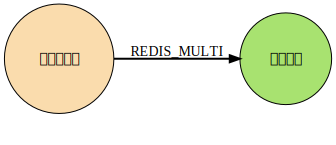
\includegraphics{graphviz-0ff9f2e58803dbb8c1c400e1f8191f77d4c2917e.pdf}


\subsection{命令入队}
\label{feature/transaction:id4}
当客户端处于非事务状态下时,
所有发送给服务器端的命令都会立即被服务器执行:

\begin{Verbatim}[commandchars=\\\{\}]
\PYG{n}{redis}\PYG{o}{\PYGZgt{}} \PYG{n}{SET} \PYG{n}{msg} \PYG{l+s}{"}\PYG{l+s}{hello moto}\PYG{l+s}{"}
\PYG{n}{OK}

\PYG{n}{redis}\PYG{o}{\PYGZgt{}} \PYG{n}{GET} \PYG{n}{msg}
\PYG{l+s}{"}\PYG{l+s}{hello moto}\PYG{l+s}{"}
\end{Verbatim}

但是,
当客户端进入事务状态之后,
服务器在收到来自客户端的命令时,
不会立即执行命令,
而是将这些命令全部放进一个事务队列里,
然后返回 \code{QUEUED} ,
表示命令已入队:

\begin{Verbatim}[commandchars=\\\{\}]
\PYG{n}{redis}\PYG{o}{\PYGZgt{}} \PYG{n}{MULTI}
\PYG{n}{OK}

\PYG{n}{redis}\PYG{o}{\PYGZgt{}} \PYG{n}{SET} \PYG{n}{msg} \PYG{l+s}{"}\PYG{l+s}{hello moto}\PYG{l+s}{"}
\PYG{n}{QUEUED}

\PYG{n}{redis}\PYG{o}{\PYGZgt{}} \PYG{n}{GET} \PYG{n}{msg}
\PYG{n}{QUEUED}
\end{Verbatim}

以下流程图展示了这一行为:

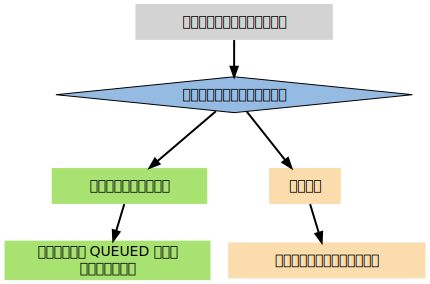
\includegraphics{graphviz-8a0f8eae0bb8180e877b799921dd690267c2d3b4.pdf}

事务队列是一个数组,
每个数组项是都包含三个属性:
\begin{enumerate}
\item {} 
要执行的命令(cmd)。

\item {} 
命令的参数(argv)。

\item {} 
参数的个数(argc)。

\end{enumerate}

举个例子,
如果客户端执行以下命令:

\begin{Verbatim}[commandchars=\\\{\}]
\PYG{n}{redis}\PYG{o}{\PYGZgt{}} \PYG{n}{MULTI}
\PYG{n}{OK}

\PYG{n}{redis}\PYG{o}{\PYGZgt{}} \PYG{n}{SET} \PYG{n}{book}\PYG{o}{-}\PYG{n}{name} \PYG{l+s}{"}\PYG{l+s}{Mastering C++ in 21 days}\PYG{l+s}{"}
\PYG{n}{QUEUED}

\PYG{n}{redis}\PYG{o}{\PYGZgt{}} \PYG{n}{GET} \PYG{n}{book}\PYG{o}{-}\PYG{n}{name}
\PYG{n}{QUEUED}

\PYG{n}{redis}\PYG{o}{\PYGZgt{}} \PYG{n}{SADD} \PYG{n}{tag} \PYG{l+s}{"}\PYG{l+s}{C++}\PYG{l+s}{"} \PYG{l+s}{"}\PYG{l+s}{Programming}\PYG{l+s}{"} \PYG{l+s}{"}\PYG{l+s}{Mastering Series}\PYG{l+s}{"}
\PYG{n}{QUEUED}

\PYG{n}{redis}\PYG{o}{\PYGZgt{}} \PYG{n}{SMEMBERS} \PYG{n}{tag}
\PYG{n}{QUEUED}
\end{Verbatim}

那么程序将为客户端创建以下事务队列:

\begin{tabulary}{\linewidth}{|L|L|L|L|}
\hline
\textbf{
数组索引
} & \textbf{
cmd
} & \textbf{
argv
} & \textbf{
argc
}\\\hline

\code{0}
 & 
\code{SET}
 & 
\code{{[}"book-name", "Mastering C++ in 21 days"{]}}
 & 
\code{2}
\\\hline

\code{1}
 & 
\code{GET}
 & 
\code{{[}"book-name"{]}}
 & 
\code{1}
\\\hline

\code{2}
 & 
\code{SADD}
 & 
\code{{[}"tag", "C++", "Programming", "Mastering Series"{]}}
 & 
\code{4}
\\\hline

\code{3}
 & 
\code{SMEMBERS}
 & 
\code{{[}"tag"{]}}
 & 
\code{1}
\\\hline
\end{tabulary}



\subsection{执行事务}
\label{feature/transaction:id5}
前面说到,
当客户端进入事务状态之后,
客户端发送的命令就会被放进事务队列里。

但其实并不是所有的命令都会被放进事务队列,
其中的例外就是 \href{http://redis.readthedocs.org/en/latest/transaction/exec.html\#exec}{\emph{EXEC}} 、 \href{http://redis.readthedocs.org/en/latest/transaction/discard.html\#discard}{\emph{DISCARD}} 、 \href{http://redis.readthedocs.org/en/latest/transaction/multi.html\#multi}{\emph{MULTI}} 和 \href{http://redis.readthedocs.org/en/latest/transaction/watch.html\#watch}{\emph{WATCH}} 这四个命令 ——
当这四个命令从客户端发送到服务器时,
它们会像客户端处于非事务状态一样,
直接被服务器执行:

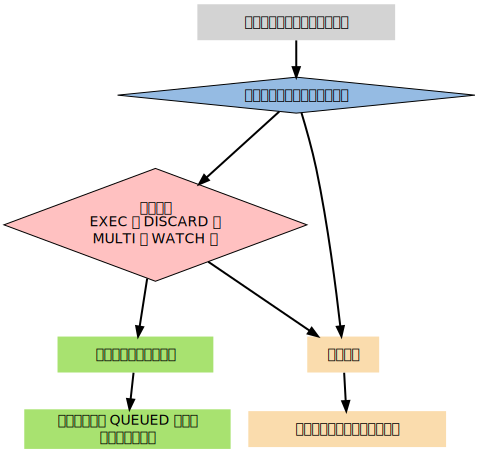
\includegraphics{graphviz-836c8a3dc33526a649d9ecf5b7b959d72b38cc7d.pdf}

如果客户端正处于事务状态,
那么当 \href{http://redis.readthedocs.org/en/latest/transaction/exec.html\#exec}{\emph{EXEC}} 命令执行时,
服务器根据客户端所保存的事务队列,
以先进先出(FIFO)的方式执行事务队列中的命令:
最先入队的命令最先执行,
而最后入队的命令最后执行。

比如说,对于以下事务队列:

\begin{tabulary}{\linewidth}{|L|L|L|L|}
\hline
\textbf{
数组索引
} & \textbf{
cmd
} & \textbf{
argv
} & \textbf{
argc
}\\\hline

\code{0}
 & 
\code{SET}
 & 
\code{{[}"book-name", "Mastering C++ in 21 days"{]}}
 & 
\code{2}
\\\hline

\code{1}
 & 
\code{GET}
 & 
\code{{[}"book-name"{]}}
 & 
\code{1}
\\\hline

\code{2}
 & 
\code{SADD}
 & 
\code{{[}"tag", "C++", "Programming", "Mastering Series"{]}}
 & 
\code{4}
\\\hline

\code{3}
 & 
\code{SMEMBERS}
 & 
\code{{[}"tag"{]}}
 & 
\code{1}
\\\hline
\end{tabulary}


程序会首先执行 \href{http://redis.readthedocs.org/en/latest/string/set.html\#set}{\emph{SET}} 命令,
然后执行 \href{http://redis.readthedocs.org/en/latest/string/get.html\#get}{\emph{GET}} 命令,
再然后执行 \href{http://redis.readthedocs.org/en/latest/set/sadd.html\#sadd}{\emph{SADD}} 命令,
最后执行 \href{http://redis.readthedocs.org/en/latest/set/smembers.html\#smembers}{\emph{SMEMBERS}} 命令。

执行事务中的命令所得的结果会以 FIFO 的顺序保存到一个回复队列中。

比如说,对于上面给出的事务队列,程序将为队列中的命令创建如下回复队列:

\begin{tabulary}{\linewidth}{|L|L|L|}
\hline
\textbf{
数组索引
} & \textbf{
回复类型
} & \textbf{
回复内容
}\\\hline

\code{0}
 & 
status code reply
 & 
\code{OK}
\\\hline

\code{1}
 & 
bulk reply
 & 
\code{"Mastering C++ in 21 days"}
\\\hline

\code{2}
 & 
integer reply
 & 
\code{3}
\\\hline

\code{3}
 & 
multi-bulk reply
 & 
\code{{[}"Mastering Series", "C++", "Programming"{]}}
\\\hline
\end{tabulary}


当事务队列里的所有命令被执行完之后,
\href{http://redis.readthedocs.org/en/latest/transaction/exec.html\#exec}{\emph{EXEC}} 命令会将回复队列作为自己的执行结果返回给客户端,
客户端从事务状态返回到非事务状态,
至此,
事务执行完毕。

事务的整个执行过程可以用以下伪代码表示:

\begin{Verbatim}[commandchars=\\\{\}]
\PYG{k}{def} \PYG{n+nf}{execute\PYGZus{}transaction}\PYG{p}{(}\PYG{p}{)}\PYG{p}{:}

    \PYG{c}{\PYGZsh{} 创建空白的回复队列}
    \PYG{n}{reply\PYGZus{}queue} \PYG{o}{=} \PYG{p}{[}\PYG{p}{]}

    \PYG{c}{\PYGZsh{} 取出事务队列里的所有命令、参数和参数数量}
    \PYG{k}{for} \PYG{n}{cmd}\PYG{p}{,} \PYG{n}{argv}\PYG{p}{,} \PYG{n}{argc} \PYG{o+ow}{in} \PYG{n}{client}\PYG{o}{.}\PYG{n}{transaction\PYGZus{}queue}\PYG{p}{:}

        \PYG{c}{\PYGZsh{} 执行命令,并取得命令的返回值}
        \PYG{n}{reply} \PYG{o}{=} \PYG{n}{execute\PYGZus{}redis\PYGZus{}command}\PYG{p}{(}\PYG{n}{cmd}\PYG{p}{,} \PYG{n}{argv}\PYG{p}{,} \PYG{n}{argc}\PYG{p}{)}

        \PYG{c}{\PYGZsh{} 将返回值追加到回复队列末尾}
        \PYG{n}{reply\PYGZus{}queue}\PYG{o}{.}\PYG{n}{append}\PYG{p}{(}\PYG{n}{reply}\PYG{p}{)}

    \PYG{c}{\PYGZsh{} 清除客户端的事务状态}
    \PYG{n}{clear\PYGZus{}transaction\PYGZus{}state}\PYG{p}{(}\PYG{n}{client}\PYG{p}{)}

    \PYG{c}{\PYGZsh{} 清空事务队列}
    \PYG{n}{clear\PYGZus{}transaction\PYGZus{}queue}\PYG{p}{(}\PYG{n}{client}\PYG{p}{)}

    \PYG{c}{\PYGZsh{} 将事务的执行结果返回给客户端}
    \PYG{n}{send\PYGZus{}reply\PYGZus{}to\PYGZus{}client}\PYG{p}{(}\PYG{n}{client}\PYG{p}{,} \PYG{n}{reply\PYGZus{}queue}\PYG{p}{)}
\end{Verbatim}


\subsection{在事务和非事务状态下执行命令}
\label{feature/transaction:id6}
无论在事务状态下,
还是在非事务状态下,
Redis 命令都由同一个函数执行,
所以它们共享很多服务器的一般设置,
比如 AOF 的配置、RDB 的配置,以及内存限制,等等。

不过事务中的命令和普通命令在执行上还是有一点区别的,其中最重要的两点是:
\begin{enumerate}
\item {} 
非事务状态下的命令以单个命令为单位执行,前一个命令和后一个命令的客户端不一定是同一个;

而事务状态则是以一个事务为单位,执行事务队列中的所有命令:除非当前事务执行完毕,否则服务器不会中断事务,也不会执行其他客户端的其他命令。

\item {} 
在非事务状态下,执行命令所得的结果会立即被返回给客户端;

而事务则是将所有命令的结果集合到回复队列,再作为 \href{http://redis.readthedocs.org/en/latest/transaction/exec.html\#exec}{\emph{EXEC}} 命令的结果返回给客户端。

\end{enumerate}


\subsection{事务状态下的 DISCARD 、 MULTI 和 WATCH 命令}
\label{feature/transaction:discard-multi-watch}
除了 \href{http://redis.readthedocs.org/en/latest/transaction/exec.html\#exec}{\emph{EXEC}} 之外,
服务器在客户端处于事务状态时,
不加入到事务队列而直接执行的另外三个命令是 \href{http://redis.readthedocs.org/en/latest/transaction/discard.html\#discard}{\emph{DISCARD}} 、 \href{http://redis.readthedocs.org/en/latest/transaction/multi.html\#multi}{\emph{MULTI}} 和 \href{http://redis.readthedocs.org/en/latest/transaction/watch.html\#watch}{\emph{WATCH}} 。

\href{http://redis.readthedocs.org/en/latest/transaction/discard.html\#discard}{\emph{DISCARD}} 命令用于取消一个事务,
它清空客户端的整个事务队列,
然后将客户端从事务状态调整回非事务状态,
最后返回字符串 \code{OK} 给客户端,
说明事务已被取消。

Redis 的事务是不可嵌套的,
当客户端已经处于事务状态,
而客户端又再向服务器发送 \href{http://redis.readthedocs.org/en/latest/transaction/multi.html\#multi}{\emph{MULTI}} 时,
服务器只是简单地向客户端发送一个错误,
然后继续等待其他命令的入队。
\href{http://redis.readthedocs.org/en/latest/transaction/multi.html\#multi}{\emph{MULTI}} 命令的发送不会造成整个事务失败,
也不会修改事务队列中已有的数据。

\href{http://redis.readthedocs.org/en/latest/transaction/watch.html\#watch}{\emph{WATCH}} 只能在客户端进入事务状态之前执行,
在事务状态下发送 \href{http://redis.readthedocs.org/en/latest/transaction/watch.html\#watch}{\emph{WATCH}} 命令会引发一个错误,
但它不会造成整个事务失败,
也不会修改事务队列中已有的数据(和前面处理 \href{http://redis.readthedocs.org/en/latest/transaction/multi.html\#multi}{\emph{MULTI}} 的情况一样)。


\subsection{带 WATCH 的事务}
\label{feature/transaction:watch}
\href{http://redis.readthedocs.org/en/latest/transaction/watch.html\#watch}{\emph{WATCH}} 命令用于在事务开始之前监视任意数量的键:
当调用 \href{http://redis.readthedocs.org/en/latest/transaction/exec.html\#exec}{\emph{EXEC}} 命令执行事务时,
如果任意一个被监视的键已经被其他客户端修改了,
那么整个事务不再执行,
直接返回失败。

以下示例展示了一个执行失败的事务例子:

\begin{Verbatim}[commandchars=\\\{\}]
\PYG{n}{redis}\PYG{o}{\PYGZgt{}} \PYG{n}{WATCH} \PYG{n}{name}
\PYG{n}{OK}

\PYG{n}{redis}\PYG{o}{\PYGZgt{}} \PYG{n}{MULTI}
\PYG{n}{OK}

\PYG{n}{redis}\PYG{o}{\PYGZgt{}} \PYG{n}{SET} \PYG{n}{name} \PYG{n}{peter}
\PYG{n}{QUEUED}

\PYG{n}{redis}\PYG{o}{\PYGZgt{}} \PYG{n}{EXEC}
\PYG{p}{(}\PYG{n}{nil}\PYG{p}{)}
\end{Verbatim}

以下执行序列展示了上面的例子是如何失败的:

\begin{tabulary}{\linewidth}{|L|L|L|}
\hline
\textbf{
时间
} & \textbf{
客户端 A
} & \textbf{
客户端 B
}\\\hline

T1
 & 
\code{WATCH name}
 & \\\hline

T2
 & 
\code{MULTI}
 & \\\hline

T3
 & 
\code{SET name peter}
 & \\\hline

T4
 &  & 
\code{SET name john}
\\\hline

T5
 & 
\code{EXEC}
 & \\\hline
\end{tabulary}


在时间 T4 ,客户端 B 修改了 \code{name} 键的值,
当客户端 A 在 T5 执行 \href{http://redis.readthedocs.org/en/latest/transaction/exec.html\#exec}{\emph{EXEC}} 时,Redis 会发现 \code{name} 这个被监视的键已经被修改,
因此客户端 A 的事务不会被执行,而是直接返回失败。

下文就来介绍 \href{http://redis.readthedocs.org/en/latest/transaction/watch.html\#watch}{\emph{WATCH}} 的实现机制,并且看看事务系统是如何检查某个被监视的键是否被修改,从而保证事务的安全性的。


\subsection{WATCH 命令的实现}
\label{feature/transaction:id7}
在每个代表数据库的 \code{redis.h/redisDb} 结构类型中,
都保存了一个 \code{watched\_keys} 字典,
字典的键是这个数据库被监视的键,
而字典的值则是一个链表,
链表中保存了所有监视这个键的客户端。

比如说,以下字典就展示了一个 \code{watched\_keys} 字典的例子:

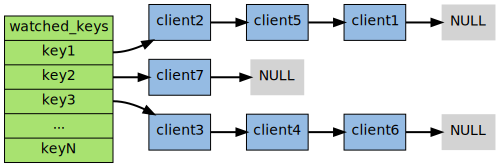
\includegraphics{graphviz-9aea81f33da1373550c590eb0b7ca0c2b3d38366.pdf}

其中, 键 \code{key1} 正在被 \code{client2} 、 \code{client5} 和 \code{client1} 三个客户端监视,
其他一些键也分别被其他别的客户端监视着。

\href{http://redis.readthedocs.org/en/latest/transaction/watch.html\#watch}{\emph{WATCH}} 命令的作用,
就是将当前客户端和要监视的键在 \code{watched\_keys} 中进行关联。

举个例子,
如果当前客户端为 \code{client10086} ,
那么当客户端执行 \code{WATCH key1 key2} 时,
前面展示的 \code{watched\_keys} 将被修改成这个样子:

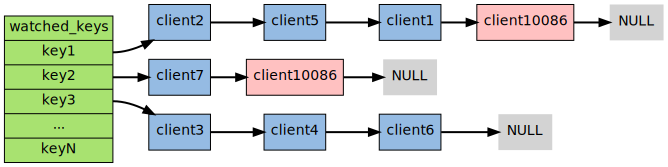
\includegraphics{graphviz-fe5e31054c282a3cdd86656994fe1678a3d4f201.pdf}

通过 \code{watched\_keys} 字典,
如果程序想检查某个键是否被监视,
那么它只要检查字典中是否存在这个键即可;
如果程序要获取监视某个键的所有客户端,
那么只要取出键的值(一个链表),
然后对链表进行遍历即可。


\subsection{WATCH 的触发}
\label{feature/transaction:id8}
在任何对数据库键空间(key space)进行修改的命令成功执行之后
(比如 \href{http://redis.readthedocs.org/en/latest/server/flushdb.html\#flushdb}{\emph{FLUSHDB}} 、 \href{http://redis.readthedocs.org/en/latest/string/set.html\#set}{\emph{SET}} 、 \href{http://redis.readthedocs.org/en/latest/key/del.html\#del}{\emph{DEL}} 、 \href{http://redis.readthedocs.org/en/latest/list/lpush.html\#lpush}{\emph{LPUSH}} 、 \href{http://redis.readthedocs.org/en/latest/set/sadd.html\#sadd}{\emph{SADD}} 、 \href{http://redis.readthedocs.org/en/latest/sorted\_set/zrem.html\#zrem}{\emph{ZREM}} ,诸如此类),
\code{multi.c/touchWatchKey} 函数都会被调用 ——
它检查数据库的 \code{watched\_keys} 字典,
看是否有客户端在监视已经被命令修改的键,
如果有的话,
程序将所有监视这个/这些被修改键的客户端的 \code{REDIS\_DIRTY\_CAS} 选项打开:

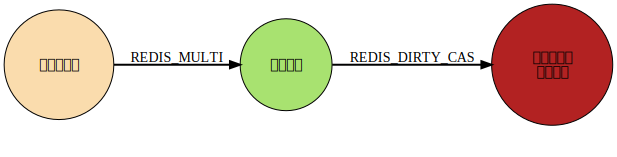
\includegraphics{graphviz-e5c66122242aa10939b696dfeeb905343c5202bd.pdf}

当客户端发送 \href{http://redis.readthedocs.org/en/latest/transaction/exec.html\#exec}{\emph{EXEC}} 命令、触发事务执行时,
服务器会对客户端的状态进行检查:
\begin{itemize}
\item {} 
如果客户端的 \code{REDIS\_DIRTY\_CAS} 选项已经被打开,那么说明被客户端监视的键至少有一个已经被修改了,事务的安全性已经被破坏。服务器会放弃执行这个事务,直接向客户端返回空回复,表示事务执行失败。

\item {} 
如果 \code{REDIS\_DIRTY\_CAS} 选项没有被打开,那么说明所有监视键都安全,服务器正式执行事务。

\end{itemize}

可以用一段伪代码来表示这个检查:

\begin{Verbatim}[commandchars=\\\{\}]
\PYG{k}{def} \PYG{n+nf}{check\PYGZus{}safety\PYGZus{}before\PYGZus{}execute\PYGZus{}trasaction}\PYG{p}{(}\PYG{p}{)}\PYG{p}{:}

    \PYG{k}{if} \PYG{n}{client}\PYG{o}{.}\PYG{n}{state} \PYG{o}{\PYGZam{}}\PYG{o}{\PYGZam{}} \PYG{n}{REDIS\PYGZus{}DIRTY\PYGZus{}CAS}\PYG{p}{:}
        \PYG{c}{\PYGZsh{} 安全性已破坏,清除事务状态}
        \PYG{n}{clear\PYGZus{}transaction\PYGZus{}state}\PYG{p}{(}\PYG{n}{client}\PYG{p}{)}
        \PYG{c}{\PYGZsh{} 清空事务队列}
        \PYG{n}{clear\PYGZus{}transaction\PYGZus{}queue}\PYG{p}{(}\PYG{n}{client}\PYG{p}{)}
        \PYG{c}{\PYGZsh{} 返回空回复给客户端}
        \PYG{n}{send\PYGZus{}empty\PYGZus{}reply}\PYG{p}{(}\PYG{n}{client}\PYG{p}{)}
    \PYG{k}{else}
        \PYG{c}{\PYGZsh{} 安全性完好,执行事务}
        \PYG{n}{execute\PYGZus{}transaction}\PYG{p}{(}\PYG{p}{)}
\end{Verbatim}

举个例子,假设数据库的 \code{watched\_keys} 字典如下图所示:

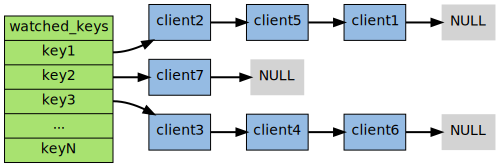
\includegraphics{graphviz-9aea81f33da1373550c590eb0b7ca0c2b3d38366.pdf}

如果某个客户端对 \code{key1} 进行了修改(比如执行 \code{DEL key1} ),
那么所有监视 \code{key1} 的客户端,
包括 \code{client2} 、 \code{client5} 和 \code{client1} 的 \code{REDIS\_DIRTY\_CAS} 选项都会被打开,
当客户端 \code{client2} 、 \code{client5} 和 \code{client1} 执行 \href{http://redis.readthedocs.org/en/latest/transaction/exec.html\#exec}{\emph{EXEC}} 的时候,
它们的事务都会以失败告终。

最后,当一个客户端结束它的事务时,无论事务是成功执行,还是失败, \code{watched\_keys} 字典中和这个客户端相关的资料都会被清除。


\subsection{事务的 ACID 性质}
\label{feature/transaction:acid}
在传统的关系式数据库中,常常用 \href{http://en.wikipedia.org/wiki/ACID}{ACID 性质}来检验事务功能的安全性。

Redis 事务保证了其中的一致性(C)和隔离性(I),但并不保证原子性(A)和持久性(D)。

以下四小节是关于这四个性质的详细讨论。


\subsubsection{原子性(Atomicity)}
\label{feature/transaction:atomicity}
单个 Redis 命令的执行是原子性的,但 Redis 没有在事务上增加任何维持原子性的机制,所以 Redis 事务的执行并不是原子性的。

如果一个事务队列中的所有命令都被成功地执行,那么称这个事务执行成功。

另一方面,如果 Redis 服务器进程在执行事务的过程中被停止 —— 比如接到 KILL 信号、宿主机器停机,等等,那么事务执行失败。

当事务失败时,Redis 也不会进行任何的重试或者回滚动作。


\subsubsection{一致性(Consistency)}
\label{feature/transaction:consistency}
Redis 的一致性问题可以分为三部分来讨论:入队错误、执行错误、Redis 进程被终结。


\paragraph{入队错误}
\label{feature/transaction:id10}
在命令入队的过程中,如果客户端向服务器发送了错误的命令,比如命令的参数数量不对,等等,
那么服务器将向客户端返回一个出错信息,
并且将客户端的事务状态设为 \code{REDIS\_DIRTY\_EXEC} 。

当客户端执行 \href{http://redis.readthedocs.org/en/latest/transaction/exec.html\#exec}{\emph{EXEC}} 命令时,
Redis 会拒绝执行状态为 \code{REDIS\_DIRTY\_EXEC} 的事务,
并返回失败信息。

\begin{Verbatim}[commandchars=\\\{\}]
redis 127.0.0.1:6379\textgreater{} MULTI
OK

redis 127.0.0.1:6379\textgreater{} set key
(error) ERR wrong number of arguments for 'set' command

redis 127.0.0.1:6379\textgreater{} EXISTS key
QUEUED

redis 127.0.0.1:6379\textgreater{} EXEC
(error) EXECABORT Transaction discarded because of previous errors.
\end{Verbatim}

因此,带有不正确入队命令的事务不会被执行,也不会影响数据库的一致性。


\paragraph{执行错误}
\label{feature/transaction:id11}
如果命令在事务执行的过程中发生错误,比如说,对一个不同类型的 key 执行了错误的操作,
那么 Redis 只会将错误包含在事务的结果中,
这不会引起事务中断或整个失败,不会影响已执行事务命令的结果,也不会影响后面要执行的事务命令,
所以它对事务的一致性也没有影响。


\paragraph{Redis 进程被终结}
\label{feature/transaction:redis}
如果 Redis 服务器进程在执行事务的过程中被其他进程终结,或者被管理员强制杀死,那么根据 Redis 所使用的持久化模式,可能有以下情况出现:
\begin{itemize}
\item {} 
内存模式:如果 Redis 没有采取任何持久化机制,那么重启之后的数据库总是空白的,所以数据总是一致的。

\item {} 
RDB 模式:在执行事务时,Redis 不会中断事务去执行保存 RDB 的工作,只有在事务执行之后,保存 RDB 的工作才有可能开始。所以当 RDB 模式下的 Redis 服务器进程在事务中途被杀死时,事务内执行的命令,不管成功了多少,都不会被保存到 RDB 文件里。恢复数据库需要使用现有的 RDB 文件,而这个 RDB 文件的数据保存的是最近一次的数据库快照(snapshot),所以它的数据可能不是最新的,但只要 RDB 文件本身没有因为其他问题而出错,那么还原后的数据库就是一致的。

\item {} 
AOF 模式:因为保存 AOF 文件的工作在后台线程进行,所以即使是在事务执行的中途,保存 AOF 文件的工作也可以继续进行,因此,根据事务语句是否被写入并保存到 AOF 文件,有以下两种情况发生:

1)如果事务语句未写入到 AOF 文件,或 AOF 未被 SYNC 调用保存到磁盘,那么当进程被杀死之后,Redis 可以根据最近一次成功保存到磁盘的 AOF 文件来还原数据库,只要 AOF 文件本身没有因为其他问题而出错,那么还原后的数据库总是一致的,但其中的数据不一定是最新的。

2)如果事务的部分语句被写入到 AOF 文件,并且 AOF 文件被成功保存,那么不完整的事务执行信息就会遗留在 AOF 文件里,当重启 Redis 时,程序会检测到 AOF 文件并不完整,Redis 会退出,并报告错误。需要使用 redis-check-aof 工具将部分成功的事务命令移除之后,才能再次启动服务器。还原之后的数据总是一致的,而且数据也是最新的(直到事务执行之前为止)。

\end{itemize}


\subsubsection{隔离性(Isolation)}
\label{feature/transaction:isolation}
Redis 是单进程程序,并且它保证在执行事务时,不会对事务进行中断,事务可以运行直到执行完所有事务队列中的命令为止。因此,Redis 的事务是总是带有隔离性的。


\subsubsection{持久性(Durability)}
\label{feature/transaction:durability}
因为事务不过是用队列包裹起了一组 Redis 命令,并没有提供任何额外的持久性功能,所以事务的持久性由 Redis 所使用的持久化模式决定:
\begin{itemize}
\item {} 
在单纯的内存模式下,事务肯定是不持久的。

\item {} 
在 RDB 模式下,服务器可能在事务执行之后、RDB 文件更新之前的这段时间失败,所以 RDB 模式下的 Redis 事务也是不持久的。

\item {} 
在 AOF 的“总是 SYNC ”模式下,事务的每条命令在执行成功之后,都会立即调用 \code{fsync} 或 \code{fdatasync} 将事务数据写入到 AOF 文件。但是,这种保存是由后台线程进行的,主线程不会阻塞直到保存成功,所以从命令执行成功到数据保存到硬盘之间,还是有一段非常小的间隔,所以这种模式下的事务也是不持久的。

其他 AOF 模式也和“总是 SYNC ”模式类似,所以它们都是不持久的。

\end{itemize}


\subsection{小结}
\label{feature/transaction:id12}\begin{itemize}
\item {} 
事务提供了一种将多个命令打包,然后一次性、有序地执行的机制。

\item {} 
事务在执行过程中不会被中断,所有事务命令执行完之后,事务才能结束。

\item {} 
多个命令会被入队到事务队列中,然后按先进先出(FIFO)的顺序执行。

\item {} 
带 \code{WATCH} 命令的事务会将客户端和被监视的键在数据库的 \code{watched\_keys} 字典中进行关联,当键被修改时,程序会将所有监视被修改键的客户端的 \code{REDIS\_DIRTY\_CAS} 选项打开。

\item {} 
只有在客户端的 \code{REDIS\_DIRTY\_CAS} 选项未被打开时,才能执行事务,否则事务直接返回失败。

\item {} 
Redis 的事务保证了 ACID 中的一致性(C)和隔离性(I),但并不保证原子性(A)和持久性(D)。

\end{itemize}


\section{订阅与发布}
\label{feature/pubsub::doc}\label{feature/pubsub:id1}
Redis 通过 \href{http://redis.readthedocs.org/en/latest/pub\_sub/publish.html\#publish}{\emph{PUBLISH}} 、 \href{http://redis.readthedocs.org/en/latest/pub\_sub/subscribe.html\#subscribe}{\emph{SUBSCRIBE}} 等命令实现了订阅与发布模式,
这个功能提供两种信息机制,
分别是订阅/发布到频道和订阅/发布到模式,
下文先讨论订阅/发布到频道的实现,
再讨论订阅/发布到模式的实现。


\subsection{频道的订阅与信息发送}
\label{feature/pubsub:id2}
Redis 的 \href{http://redis.readthedocs.org/en/latest/pub\_sub/subscribe.html\#subscribe}{\emph{SUBSCRIBE}} 命令可以让客户端订阅任意数量的频道,
每当有新信息发送到被订阅的频道时,
信息就会被发送给所有订阅指定频道的客户端。

作为例子,
下图展示了频道 \code{channel1} ,
以及订阅这个频道的三个客户端 —— \code{client2} 、 \code{client5} 和 \code{client1} 之间的关系:

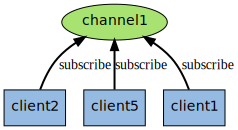
\includegraphics{graphviz-58f7b1f1f52b28f59291d194555fc9f4b1462a4c.pdf}

当有新消息通过 \href{http://redis.readthedocs.org/en/latest/pub\_sub/publish.html\#publish}{\emph{PUBLISH}} 命令发送给频道 \code{channel1} 时,
这个消息就会被发送给订阅它的三个客户端:

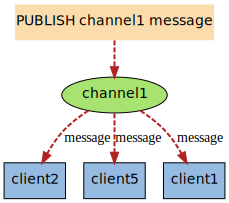
\includegraphics{graphviz-84c95abf88d6c0ac55b007da08805a4b9a582fdf.pdf}

在后面的内容中,
我们将探讨 \href{http://redis.readthedocs.org/en/latest/pub\_sub/subscribe.html\#subscribe}{\emph{SUBSCRIBE}} 和 \href{http://redis.readthedocs.org/en/latest/pub\_sub/publish.html\#publish}{\emph{PUBLISH}} 命令的实现,
以及这套订阅与发布机制的运作原理。


\subsection{订阅频道}
\label{feature/pubsub:id3}
每个 Redis 服务器进程都维持着一个表示服务器状态的 \code{redis.h/redisServer} 结构,
结构的 \code{pubsub\_channels} 属性是一个字典,
这个字典就用于保存订阅频道的信息:

\begin{Verbatim}[commandchars=\\\{\}]
\PYG{k}{struct} \PYG{n}{redisServer} \PYG{p}{\PYGZob{}}
    \PYG{c+c1}{// ...}
    \PYG{n}{dict} \PYG{o}{*}\PYG{n}{pubsub\PYGZus{}channels}\PYG{p}{;}
    \PYG{c+c1}{// ...}
\PYG{p}{\PYGZcb{}}\PYG{p}{;}
\end{Verbatim}

其中,字典的键为正在被订阅的频道,
而字典的值则是一个链表,
链表中保存了所有订阅这个频道的客户端。

比如说,在下图展示的这个 \code{pubsub\_channels} 示例中, \code{client2} 、 \code{client5} 和 \code{client1} 就订阅了 \code{channel1} ,
而其他频道也分别被别的客户端所订阅:

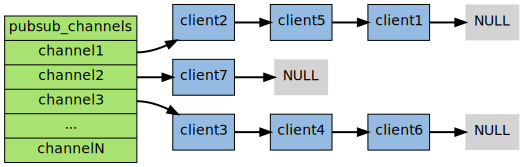
\includegraphics{graphviz-241c988b86bb9bed6bf26537e654baaab4eef77b.pdf}

当客户端调用 \href{http://redis.readthedocs.org/en/latest/pub\_sub/subscribe.html\#subscribe}{\emph{SUBSCRIBE}} 命令时,
程序就将客户端和要订阅的频道在 \code{pubsub\_channels} 字典中关联起来。

举个例子,如果客户端 \code{client10086} 执行命令 \code{SUBSCRIBE channel1 channel2 channel3} ,那么前面展示的 \code{pubsub\_channels} 将变成下面这个样子:

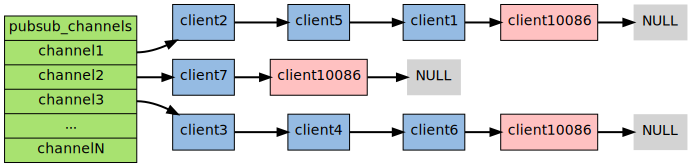
\includegraphics{graphviz-cb250b1be4aaaedc9d5ddde113a80998d7f9c480.pdf}

\href{http://redis.readthedocs.org/en/latest/pub\_sub/subscribe.html\#subscribe}{\emph{SUBSCRIBE}} 命令的行为可以用伪代码表示如下:

\begin{Verbatim}[commandchars=\\\{\}]
\PYG{k}{def} \PYG{n+nf}{SUBSCRIBE}\PYG{p}{(}\PYG{n}{client}\PYG{p}{,} \PYG{n}{channels}\PYG{p}{)}\PYG{p}{:}

    \PYG{c}{\PYGZsh{} 遍历所有输入频道}
    \PYG{k}{for} \PYG{n}{channel} \PYG{o+ow}{in} \PYG{n}{channels}\PYG{p}{:}

        \PYG{c}{\PYGZsh{} 将客户端添加到链表的末尾}
        \PYG{n}{redisServer}\PYG{o}{.}\PYG{n}{pubsub\PYGZus{}channels}\PYG{p}{[}\PYG{n}{channel}\PYG{p}{]}\PYG{o}{.}\PYG{n}{append}\PYG{p}{(}\PYG{n}{client}\PYG{p}{)}
\end{Verbatim}

通过 \code{pubsub\_channels} 字典,
程序只要检查某个频道是否字典的键,
就可以知道该频道是否正在被客户端订阅;
只要取出某个键的值,
就可以得到所有订阅该频道的客户端的信息。


\subsection{发送信息到频道}
\label{feature/pubsub:id4}
了解了 \code{pubsub\_channels} 字典的结构之后,
解释 \href{http://redis.readthedocs.org/en/latest/pub\_sub/publish.html\#publish}{\emph{PUBLISH}} 命令的实现就非常简单了:
当调用 \code{PUBLISH channel message} 命令,
程序首先根据 \code{channel} 定位到字典的键,
然后将信息发送给字典值链表中的所有客户端。

比如说,对于以下这个 \code{pubsub\_channels} 实例,
如果某个客户端执行命令 \code{PUBLISH channel1 "hello moto"} ,那么 \code{client2} 、 \code{client5} 和 \code{client1} 三个客户端都将接收到 \code{"hello moto"} 信息:

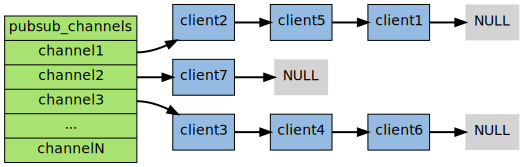
\includegraphics{graphviz-241c988b86bb9bed6bf26537e654baaab4eef77b.pdf}

\href{http://redis.readthedocs.org/en/latest/pub\_sub/publish.html\#publish}{\emph{PUBLISH}} 命令的实现可以用以下伪代码来描述:

\begin{Verbatim}[commandchars=\\\{\}]
\PYG{k}{def} \PYG{n+nf}{PUBLISH}\PYG{p}{(}\PYG{n}{channel}\PYG{p}{,} \PYG{n}{message}\PYG{p}{)}\PYG{p}{:}

    \PYG{c}{\PYGZsh{} 遍历所有订阅频道 channel 的客户端}
    \PYG{k}{for} \PYG{n}{client} \PYG{o+ow}{in} \PYG{n}{server}\PYG{o}{.}\PYG{n}{pubsub\PYGZus{}channels}\PYG{p}{[}\PYG{n}{channel}\PYG{p}{]}\PYG{p}{:}

        \PYG{c}{\PYGZsh{} 将信息发送给它们}
        \PYG{n}{send\PYGZus{}message}\PYG{p}{(}\PYG{n}{client}\PYG{p}{,} \PYG{n}{message}\PYG{p}{)}
\end{Verbatim}


\subsection{退订频道}
\label{feature/pubsub:id5}
使用 \href{http://redis.readthedocs.org/en/latest/pub\_sub/unsubscribe.html\#unsubscribe}{\emph{UNSUBSCRIBE}} 命令可以退订指定的频道,
这个命令执行的是订阅的反操作:
它从 \code{pubsub\_channels} 字典的给定频道(键)中,
删除关于当前客户端的信息,
这样被退订频道的信息就不会再发送给这个客户端。


\subsection{模式的订阅与信息发送}
\label{feature/pubsub:id6}
当使用 \href{http://redis.readthedocs.org/en/latest/pub\_sub/publish.html\#publish}{\emph{PUBLISH}} 命令发送信息到某个频道时,
不仅所有订阅该频道的客户端会收到信息,
如果有某个/某些模式和这个频道匹配的话,
那么所有订阅这个/这些频道的客户端也同样会收到信息。

下图展示了一个带有频道和模式的例子,
其中 \code{tweet.shop.*} 模式匹配了 \code{tweet.shop.kindle} 频道和 \code{tweet.shop.ipad} 频道,
并且有不同的客户端分别订阅它们三个:

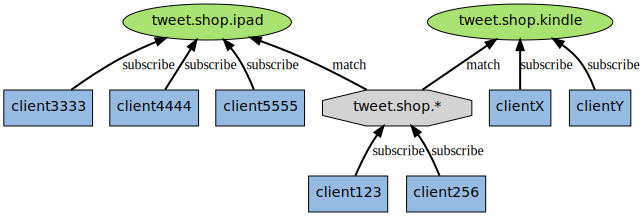
\includegraphics{graphviz-49c2b60cc3c2b52ec1623fbd8a9002eb6f335a54.pdf}

当有信息发送到 \code{tweet.shop.kindle} 频道时,
信息除了发送给 \code{clientX} 和 \code{clientY} 之外,
还会发送给订阅 \code{tweet.shop.*} 模式的 \code{client123} 和 \code{client256} :

\includegraphics{graphviz-3d1f513ee0718a326d53152b2b97f82977e38ad6.pdf}

另一方面,
如果接收到信息的是频道 \code{tweet.shop.ipad} ,
那么 \code{client123} 和 \code{client256} 同样会收到信息:

\includegraphics{graphviz-ba8c4d4dd538464659aeb52d6c366f23ad3d0dc1.pdf}


\subsection{订阅模式}
\label{feature/pubsub:id7}
\code{redisServer.pubsub\_patterns} 属性是一个链表,链表中保存着所有和模式相关的信息:

\begin{Verbatim}[commandchars=\\\{\}]
\PYG{k}{struct} \PYG{n}{redisServer} \PYG{p}{\PYGZob{}}
    \PYG{c+c1}{// ...}
    \PYG{n}{list} \PYG{o}{*}\PYG{n}{pubsub\PYGZus{}patterns}\PYG{p}{;}
    \PYG{c+c1}{// ...}
\PYG{p}{\PYGZcb{}}\PYG{p}{;}
\end{Verbatim}

链表中的每个节点都包含一个 \code{redis.h/pubsubPattern} 结构:

\begin{Verbatim}[commandchars=\\\{\}]
\PYG{k}{typedef} \PYG{k}{struct} \PYG{n}{pubsubPattern} \PYG{p}{\PYGZob{}}
    \PYG{n}{redisClient} \PYG{o}{*}\PYG{n}{client}\PYG{p}{;}
    \PYG{n}{robj} \PYG{o}{*}\PYG{n}{pattern}\PYG{p}{;}
\PYG{p}{\PYGZcb{}} \PYG{n}{pubsubPattern}\PYG{p}{;}
\end{Verbatim}

\code{client} 属性保存着订阅模式的客户端,而 \code{pattern} 属性则保存着被订阅的模式。

每当调用 \code{PSUBSCRIBE} 命令订阅一个模式时,
程序就创建一个包含客户端信息和被订阅模式的 \code{pubsubPattern} 结构,
并将该结构添加到 \code{redisServer.pubsub\_patterns} 链表中。

作为例子,下图展示了一个包含两个模式的 \code{pubsub\_patterns} 链表,
其中 \code{client123} 和 \code{client256} 都正在订阅 \code{tweet.shop.*} 模式:

\includegraphics{graphviz-b8d101c1b582531bce2b0daef87adbaf30ebc195.pdf}

如果这时客户端 \code{client10086} 执行 \code{PSUBSCRIBE broadcast.list.*} ,
那么 \code{pubsub\_patterns} 链表将被更新成这样:

\includegraphics{graphviz-a84f3abf466ca19297faaa4e11d37f9257355c60.pdf}

通过遍历整个 \code{pubsub\_patterns} 链表,程序可以检查所有正在被订阅的模式,以及订阅这些模式的客户端。


\subsection{发送信息到模式}
\label{feature/pubsub:id8}
发送信息到模式的工作也是由 \href{http://redis.readthedocs.org/en/latest/pub\_sub/publish.html\#publish}{\emph{PUBLISH}} 命令进行的,
在前面讲解频道的时候,
我们给出了这样一段伪代码,
说它定义了 \href{http://redis.readthedocs.org/en/latest/pub\_sub/publish.html\#publish}{\emph{PUBLISH}} 命令的行为:

\begin{Verbatim}[commandchars=\\\{\}]
\PYG{k}{def} \PYG{n+nf}{PUBLISH}\PYG{p}{(}\PYG{n}{channel}\PYG{p}{,} \PYG{n}{message}\PYG{p}{)}\PYG{p}{:}

    \PYG{c}{\PYGZsh{} 遍历所有订阅频道 channel 的客户端}
    \PYG{k}{for} \PYG{n}{client} \PYG{o+ow}{in} \PYG{n}{server}\PYG{o}{.}\PYG{n}{pubsub\PYGZus{}channels}\PYG{p}{[}\PYG{n}{channel}\PYG{p}{]}\PYG{p}{:}

        \PYG{c}{\PYGZsh{} 将信息发送给它们}
        \PYG{n}{send\PYGZus{}message}\PYG{p}{(}\PYG{n}{client}\PYG{p}{,} \PYG{n}{message}\PYG{p}{)}
\end{Verbatim}

但是,这段伪代码并没有完整描述 \href{http://redis.readthedocs.org/en/latest/pub\_sub/publish.html\#publish}{\emph{PUBLISH}} 命令的行为,
因为 \href{http://redis.readthedocs.org/en/latest/pub\_sub/publish.html\#publish}{\emph{PUBLISH}} 除了将 \code{message} 发送到所有订阅 \code{channel} 的客户端之外,
它还会将 \code{channel} 和 \code{pubsub\_patterns} 中的模式进行对比,
如果 \code{channel} 和某个模式匹配的话,
那么也将 \code{message} 发送到订阅那个模式的客户端。

完整描述 \href{http://redis.readthedocs.org/en/latest/pub\_sub/publish.html\#publish}{\emph{PUBLISH}} 功能的伪代码定于如下:

\begin{Verbatim}[commandchars=\\\{\}]
\PYG{k}{def} \PYG{n+nf}{PUBLISH}\PYG{p}{(}\PYG{n}{channel}\PYG{p}{,} \PYG{n}{message}\PYG{p}{)}\PYG{p}{:}

    \PYG{c}{\PYGZsh{} 遍历所有订阅频道 channel 的客户端}
    \PYG{k}{for} \PYG{n}{client} \PYG{o+ow}{in} \PYG{n}{server}\PYG{o}{.}\PYG{n}{pubsub\PYGZus{}channels}\PYG{p}{[}\PYG{n}{channel}\PYG{p}{]}\PYG{p}{:}

        \PYG{c}{\PYGZsh{} 将信息发送给它们}
        \PYG{n}{send\PYGZus{}message}\PYG{p}{(}\PYG{n}{client}\PYG{p}{,} \PYG{n}{message}\PYG{p}{)}

    \PYG{c}{\PYGZsh{} 取出所有模式,以及订阅模式的客户端}
    \PYG{k}{for} \PYG{n}{pattern}\PYG{p}{,} \PYG{n}{client} \PYG{o+ow}{in} \PYG{n}{server}\PYG{o}{.}\PYG{n}{pubsub\PYGZus{}patterns}\PYG{p}{:}

        \PYG{c}{\PYGZsh{} 如果 channel 和模式匹配}
        \PYG{k}{if} \PYG{n}{match}\PYG{p}{(}\PYG{n}{channel}\PYG{p}{,} \PYG{n}{pattern}\PYG{p}{)}\PYG{p}{:}

            \PYG{c}{\PYGZsh{} 那么也将信息发给订阅这个模式的客户端}
            \PYG{n}{send\PYGZus{}message}\PYG{p}{(}\PYG{n}{client}\PYG{p}{,} \PYG{n}{message}\PYG{p}{)}
\end{Verbatim}

举个例子,如果 Redis 服务器的 \code{pubsub\_patterns} 状态如下:

\includegraphics{graphviz-a84f3abf466ca19297faaa4e11d37f9257355c60.pdf}

那么当某个客户端发送信息 \code{"Amazon Kindle, \$69."} 到 \code{tweet.shop.kindle} 频道时,
除了所有订阅了 \code{tweet.shop.kindle} 频道的客户端会收到信息之外,
客户端 \code{client123} 和 \code{client256} 也同样会收到信息,
因为这两个客户端订阅的 \code{tweet.shop.*} 模式和 \code{tweet.shop.kindle} 频道匹配。


\subsection{退订模式}
\label{feature/pubsub:id9}
使用 \href{http://redis.readthedocs.org/en/latest/pub\_sub/punsubscribe.html\#punsubscribe}{\emph{PUNSUBSCRIBE}} 命令可以退订指定的模式,
这个命令执行的是订阅模式的反操作:
程序会删除 \code{redisServer.pubsub\_patterns} 链表中,
所有和被退订模式相关联的 \code{pubsubPattern} 结构,
这样客户端就不会再收到和模式相匹配的频道发来的信息。


\subsection{小结}
\label{feature/pubsub:id10}\begin{itemize}
\item {} 
订阅信息由服务器进程维持的 \code{redisServer.pubsub\_channels} 字典保存,字典的键为被订阅的频道,字典的值为订阅频道的所有客户端。

\item {} 
当有新消息发送到频道时,程序遍历频道(键)所对应的(值)所有客户端,然后将消息发送到所有订阅频道的客户端上。

\item {} 
订阅模式的信息由服务器进程维持的 \code{redisServer.pubsub\_patterns} 链表保存,链表的每个节点都保存着一个 \code{pubsubPattern} 结构,结构中保存着被订阅的模式,以及订阅该模式的客户端。程序通过遍历链表来查找某个频道是否和某个模式匹配。

\item {} 
当有新消息发送到频道时,除了订阅频道的客户端会收到消息之外,所有订阅了匹配频道的模式的客户端,也同样会收到消息。

\item {} 
退订频道和退订模式分别是订阅频道和订阅模式的反操作。

\end{itemize}


\section{Lua 脚本}
\label{feature/scripting:lua}\label{feature/scripting::doc}
Lua 脚本功能是 Reids 2.6 版本的最大亮点,
通过内嵌对 Lua 环境的支持,
Redis 解决了长久以来不能高效地处理 CAS (check-and-set)命令的缺点,
并且可以通过组合使用多个命令,
轻松实现以前很难实现或者不能高效实现的模式。

本章先介绍 Lua 环境的初始化步骤,
然后对 Lua 脚本的安全性问题、以及解决这些问题的方法进行说明,
最后对执行 Lua 脚本的两个命令 —— \href{http://redis.readthedocs.org/en/latest/script/eval.html\#eval}{\emph{EVAL}} 和 \href{http://redis.readthedocs.org/en/latest/script/evalsha.html\#evalsha}{\emph{EVALSHA}} 的实现原理进行介绍。


\subsection{初始化 Lua 环境}
\label{feature/scripting:id1}
在初始化 Redis 服务器时,
对 Lua 环境的初始化也会一并进行。

为了让 Lua 环境符合 Redis 脚本功能的需求,
Redis 对 Lua 环境进行了一系列的修改,
包括添加函数库、更换随机函数、保护全局变量,
等等。

整个初始化 Lua 环境的步骤如下:
\begin{enumerate}
\item {} 
调用 \href{http://www.lua.org/pil/24.1.html}{lua\_open} 函数,创建一个新的 Lua 环境。

\item {} 
载入指定的 Lua 函数库,包括:
\begin{itemize}
\item {} 
基础库(base lib)。

\item {} 
表格库(table lib)。

\item {} 
字符串库(string lib)。

\item {} 
数学库(math lib)。

\item {} 
调试库(debug lib)。

\item {} 
用于处理 JSON 对象的 \code{cjson} 库。

\item {} 
在 Lua 值和 C 结构(struct)之间进行转换的 \code{struct} 库(\href{http://www.inf.puc-rio.br/~roberto/struct/}{www.inf.puc-rio.br/~roberto/struct/})

\item {} 
处理 MessagePack 数据的 \code{cmsgpack} 库(\href{https://github.com/antirez/lua-cmsgpack}{github.com/antirez/lua-cmsgpack})。

\end{itemize}

\item {} 
屏蔽一些可能对 Lua 环境产生安全问题的函数,比如 \href{http://pgl.yoyo.org/luai/i/loadfile}{loadfile} 。

\item {} 
创建一个 Redis 字典,保存 Lua 脚本,并在复制(replication)脚本时使用。字典的键为 SHA1 校验和,字典的值为 Lua 脚本。

\item {} 
创建一个 \code{redis} 全局表格到 Lua 环境,表格中包含了各种对 Redis 进行操作的函数,包括:
\begin{itemize}
\item {} 
用于执行 Redis 命令的 \code{redis.call} 和 \code{redis.pcall} 函数。

\item {} 
用于发送日志(log)的 \code{redis.log} 函数,以及相应的日志级别(level):
\begin{itemize}
\item {} 
\code{redis.LOG\_DEBUG}

\item {} 
\code{redis.LOG\_VERBOSE}

\item {} 
\code{redis.LOG\_NOTICE}

\item {} 
\code{redis.LOG\_WARNING}

\end{itemize}

\item {} 
用于计算 SHA1 校验和的 \code{redis.sha1hex} 函数。

\item {} 
用于返回错误信息的 \code{redis.error\_reply} 函数和 \code{redis.status\_reply} 函数。

\end{itemize}

\item {} 
用 Redis 自己定义的随机生成函数,替换 \code{math} 表原有的 \code{math.random} 函数和 \code{math.randomseed} 函数,新的函数具有这样的性质:每次执行 Lua 脚本时,除非显式地调用 \code{math.randomseed} ,否则 \code{math.random} 生成的伪随机数序列总是相同的。

\item {} 
创建一个对 Redis 多批量回复(multi bulk reply)进行排序的辅助函数。

\item {} 
对 Lua 环境中的全局变量进行保护,以免被传入的脚本修改。

\item {} 
因为 Redis 命令必须通过客户端来执行,所以需要在服务器状态中创建一个无网络连接的伪客户端(fake client),专门用于执行 Lua 脚本中包含的 Redis 命令:当 Lua 脚本需要执行 Redis 命令时,它通过伪客户端来向服务器发送命令请求,服务器在执行完命令之后,将结果返回给伪客户端,而伪客户端又转而将命令结果返回给 Lua 脚本。

\item {} 
将 Lua 环境的指针记录到 Redis 服务器的全局状态中,等候 Redis 的调用。

\end{enumerate}

以上就是 Redis 初始化 Lua 环境的整个过程,
当这些步骤都执行完之后,
Redis 就可以使用 Lua 环境来处理脚本了。

严格来说,
步骤 1 至 8 才是初始化 Lua 环境的操作,
而步骤 9 和 10 则是将 Lua 环境关联到服务器的操作,
为了按顺序观察整个初始化过程,
我们将两种操作放在了一起。

另外,
步骤 6 用于创建无副作用的脚本,
而步骤 7 则用于去除部分 Redis 命令中的不确定性(non deterministic),
关于这两点,
请看下面一节关于脚本安全性的讨论。


\subsection{脚本的安全性}
\label{feature/scripting:id2}
当将 Lua 脚本复制到附属节点,
或者将 Lua 脚本写入 AOF 文件时,
Redis 需要解决这样一个问题:
如果一段 Lua 脚本带有随机性质或副作用,
那么当这段脚本在附属节点运行时,
或者从 AOF 文件载入重新运行时,
它得到的结果可能和之前运行的结果完全不同。

考虑以下一段代码,
其中的 \code{get\_random\_number()} 带有随机性质,
我们在服务器 SERVER 中执行这段代码,
并将随机数的结果保存到键 \code{number} 上:

\begin{Verbatim}[commandchars=\\\{\}]
\PYG{c+cp}{\PYGZsh{}}\PYG{c+cp}{ 虚构例子,不会真的出现在脚本环境中}

\PYG{n}{redis}\PYG{o}{\PYGZgt{}} \PYG{n}{EVAL} \PYG{l+s}{"}\PYG{l+s}{return redis.call('set', KEYS[1], get\PYGZus{}random\PYGZus{}number())}\PYG{l+s}{"} \PYG{l+m+mi}{1} \PYG{n}{number}
\PYG{n}{OK}

\PYG{n}{redis}\PYG{o}{\PYGZgt{}} \PYG{n}{GET} \PYG{n}{number}
\PYG{l+s}{"}\PYG{l+s}{10086}\PYG{l+s}{"}
\end{Verbatim}

现在,
假如 \href{http://redis.readthedocs.org/en/latest/script/eval.html\#eval}{\emph{EVAL}} 的代码被复制到了附属节点 SLAVE ,
因为 \code{get\_random\_number()} 的随机性质,
它有很大可能会生成一个和 \code{10086} 完全不同的值,
比如 \code{65535} :

\begin{Verbatim}[commandchars=\\\{\}]
\PYG{c+cp}{\PYGZsh{}}\PYG{c+cp}{ 虚构例子,不会真的出现在脚本环境中}

\PYG{n}{redis}\PYG{o}{\PYGZgt{}} \PYG{n}{EVAL} \PYG{l+s}{"}\PYG{l+s}{return redis.call('set', KEYS[1], get\PYGZus{}random\PYGZus{}number())}\PYG{l+s}{"} \PYG{l+m+mi}{1} \PYG{n}{number}
\PYG{n}{OK}

\PYG{n}{redis}\PYG{o}{\PYGZgt{}} \PYG{n}{GET} \PYG{n}{number}
\PYG{l+s}{"}\PYG{l+s}{65535}\PYG{l+s}{"}
\end{Verbatim}

可以看到,
带有随机性的写入脚本产生了一个严重的问题:
它破坏了服务器和附属节点数据之间的一致性。

当从 AOF 文件中载入带有随机性质的写入脚本时,
也会发生同样的问题。

\begin{notice}{note}{Note:}
只有在带有随机性的脚本进行写入时,
随机性才是有害的。

如果一个脚本只是执行只读操作,
那么随机性是无害的。

比如说,
如果脚本只是单纯地执行 \code{RANDOMKEY} 命令,
那么它是无害的;
但如果在执行 \code{RANDOMKEY} 之后,
基于 \code{RANDOMKEY} 的结果进行写入操作,
那么这个脚本就是有害的。
\end{notice}

和随机性质类似,
如果一个脚本的执行对任何副作用产生了依赖,
那么这个脚本每次执行所产生的结果都可能会不一样。

为了解决这个问题,
Redis 对 Lua 环境所能执行的脚本做了一个严格的限制 ——
所有脚本都必须是无副作用的纯函数(pure function)。

为此,Redis 对 Lua 环境做了一些列相应的措施:
\begin{itemize}
\item {} 
不提供访问系统状态状态的库(比如系统时间库)。

\item {} 
禁止使用 \href{http://pgl.yoyo.org/luai/i/loadfile}{loadfile} 函数。

\item {} 
如果脚本在执行带有随机性质的命令(比如 \href{http://redis.readthedocs.org/en/latest/key/randomkey.html\#randomkey}{\emph{RANDOMKEY}} ),或者带有副作用的命令(比如 \href{http://redis.readthedocs.org/en/latest/server/time.html\#time}{\emph{TIME}} )之后,试图执行一个写入命令(比如 \href{http://redis.readthedocs.org/en/latest/string/set.html\#set}{\emph{SET}} ),那么 Redis 将阻止这个脚本继续运行,并返回一个错误。

\item {} 
如果脚本执行了带有随机性质的读命令(比如 \href{http://redis.readthedocs.org/en/latest/set/smembers.html\#smembers}{\emph{SMEMBERS}} ),那么在脚本的输出返回给 Redis 之前,会先被执行一个自动的\href{http://en.wikipedia.org/wiki/Lexicographical\_order}{字典序排序},从而确保输出结果是有序的。

\item {} 
用 Redis 自己定义的随机生成函数,替换 Lua 环境中 \code{math} 表原有的 \href{http://pgl.yoyo.org/luai/i/math.random}{math.random} 函数和 \href{http://pgl.yoyo.org/luai/i/math.randomseed}{math.randomseed} 函数,新的函数具有这样的性质:每次执行 Lua 脚本时,除非显式地调用 \code{math.randomseed} ,否则 \code{math.random} 生成的伪随机数序列总是相同的。

\end{itemize}

经过这一系列的调整之后,
Redis 可以保证被执行的脚本:
\begin{enumerate}
\item {} 
无副作用。

\item {} 
没有有害的随机性。

\item {} 
对于同样的输入参数和数据集,总是产生相同的写入命令。

\end{enumerate}


\subsection{脚本的执行}
\label{feature/scripting:id5}
在脚本环境的初始化工作完成以后,
Redis 就可以通过 \href{http://redis.readthedocs.org/en/latest/script/eval.html\#eval}{\emph{EVAL}} 命令或 \href{http://redis.readthedocs.org/en/latest/script/evalsha.html\#evalsha}{\emph{EVALSHA}} 命令执行 Lua 脚本了。

其中,
\href{http://redis.readthedocs.org/en/latest/script/eval.html\#eval}{\emph{EVAL}} 直接对输入的脚本代码体(body)进行求值:

\begin{Verbatim}[commandchars=\\\{\}]
\PYG{n}{redis}\PYG{o}{\PYGZgt{}} \PYG{n}{EVAL} \PYG{l+s}{"}\PYG{l+s}{return 'hello world'}\PYG{l+s}{"} \PYG{l+m+mi}{0}
\PYG{l+s}{"}\PYG{l+s}{hello world}\PYG{l+s}{"}
\end{Verbatim}

而 \href{http://redis.readthedocs.org/en/latest/script/evalsha.html\#evalsha}{\emph{EVALSHA}} 则要求输入某个脚本的 SHA1 校验和,
这个校验和所对应的脚本必须至少被 \href{http://redis.readthedocs.org/en/latest/script/eval.html\#eval}{\emph{EVAL}} 执行过一次:

\begin{Verbatim}[commandchars=\\\{\}]
\PYG{n}{redis}\PYG{o}{\PYGZgt{}} \PYG{n}{EVAL} \PYG{l+s}{"}\PYG{l+s}{return 'hello world'}\PYG{l+s}{"} \PYG{l+m+mi}{0}
\PYG{l+s}{"}\PYG{l+s}{hello world}\PYG{l+s}{"}

\PYG{n}{redis}\PYG{o}{\PYGZgt{}} \PYG{n}{EVALSHA} \PYG{l+m+mi}{5332031}\PYG{n}{c6b470dc5a0dd9b4bf2030dea6d65de91} \PYG{l+m+mi}{0}    \PYG{c+c1}{// 上一个脚本的校验和}
\PYG{l+s}{"}\PYG{l+s}{hello world}\PYG{l+s}{"}
\end{Verbatim}

或者曾经使用 \href{http://redis.readthedocs.org/en/latest/script/script\_load.html\#script-load}{\emph{SCRIPT LOAD}} 载入过这个脚本:

\begin{Verbatim}[commandchars=\\\{\}]
\PYG{n}{redis}\PYG{o}{\PYGZgt{}} \PYG{n}{SCRIPT} \PYG{n}{LOAD} \PYG{l+s}{"}\PYG{l+s}{return 'dlrow olleh'}\PYG{l+s}{"}
\PYG{l+s}{"}\PYG{l+s}{d569c48906b1f4fca0469ba4eee89149b5148092}\PYG{l+s}{"}

\PYG{n}{redis}\PYG{o}{\PYGZgt{}} \PYG{n}{EVALSHA} \PYG{n}{d569c48906b1f4fca0469ba4eee89149b5148092} \PYG{l+m+mi}{0}
\PYG{l+s}{"}\PYG{l+s}{dlrow olleh}\PYG{l+s}{"}
\end{Verbatim}

因为 \href{http://redis.readthedocs.org/en/latest/script/evalsha.html\#evalsha}{\emph{EVALSHA}} 是基于 \href{http://redis.readthedocs.org/en/latest/script/eval.html\#eval}{\emph{EVAL}} 构建的,
所以下文先用一节讲解 \href{http://redis.readthedocs.org/en/latest/script/eval.html\#eval}{\emph{EVAL}} 的实现,
之后再讲解 \href{http://redis.readthedocs.org/en/latest/script/evalsha.html\#evalsha}{\emph{EVALSHA}} 的实现。


\subsection{EVAL 命令的实现}
\label{feature/scripting:eval}
\href{http://redis.readthedocs.org/en/latest/script/eval.html\#eval}{\emph{EVAL}} 命令的执行可以分为以下步骤:
\begin{enumerate}
\item {} 
为输入脚本定义一个 Lua 函数。

\item {} 
执行这个 Lua 函数。

\end{enumerate}

以下两个小节分别介绍这两个步骤。


\subsubsection{定义 Lua 函数}
\label{feature/scripting:id6}\label{feature/scripting:define-lua-function}
所有被 Redis 执行的 Lua 脚本,
在 Lua 环境中都会有一个和该脚本相对应的无参数函数:
当调用 \href{http://redis.readthedocs.org/en/latest/script/eval.html\#eval}{\emph{EVAL}} 命令执行脚本时,
程序第一步要完成的工作就是为传入的脚本创建一个相应的 Lua 函数。

举个例子,
当执行命令 \code{EVAL "return 'hello world'" 0} 时,
Lua 会为脚本 \code{"return 'hello world'"} 创建以下函数:

\begin{Verbatim}[commandchars=\\\{\}]
\PYG{k}{function} \PYG{n+nf}{f\PYGZus{}5332031c6b470dc5a0dd9b4bf2030dea6d65de91}\PYG{p}{(}\PYG{p}{)}
    \PYG{k}{return} \PYG{l+s+s1}{'}\PYG{l+s}{h}\PYG{l+s}{e}\PYG{l+s}{l}\PYG{l+s}{l}\PYG{l+s}{o}\PYG{l+s}{ }\PYG{l+s}{w}\PYG{l+s}{o}\PYG{l+s}{r}\PYG{l+s}{l}\PYG{l+s}{d}\PYG{l+s}{'}
\PYG{k}{end}
\end{Verbatim}

其中,
函数名以 \code{f\_} 为前缀,
后跟脚本的 SHA1 校验和(一个 40 个字符长的字符串)拼接而成。
而函数体(body)则是用户输入的脚本。

以函数为单位保存 Lua 脚本有以下好处:
\begin{itemize}
\item {} 
执行脚本的步骤非常简单,只要调用和脚本相对应的函数即可。

\item {} 
Lua 环境可以保持清洁,已有的脚本和新加入的脚本不会互相干扰,也可以将重置 Lua 环境和调用 Lua GC 的次数降到最低。

\item {} 
如果某个脚本所对应的函数在 Lua 环境中被定义过至少一次,那么只要记得这个脚本的 SHA1 校验和,就可以直接执行该脚本 —— 这是实现 \href{http://redis.readthedocs.org/en/latest/script/evalsha.html\#evalsha}{\emph{EVALSHA}} 命令的基础,稍后在介绍 \href{http://redis.readthedocs.org/en/latest/script/evalsha.html\#evalsha}{\emph{EVALSHA}} 的时候就会说到这一点。

\end{itemize}

在为脚本创建函数前,程序会先用函数名检查 Lua 环境,只有在函数定义未存在时,程序才创建函数。重复定义函数一般并没有什么副作用,这算是一个小优化。

另外,如果定义的函数在编译过程中出错(比如,脚本的代码语法有错),
那么程序向用户返回一个脚本错误,
不再执行后面的步骤。


\subsubsection{执行 Lua 函数}
\label{feature/scripting:id7}
在定义好 Lua 函数之后,
程序就可以通过运行这个函数来达到运行输入脚本的目的了。

不过,
在此之前,
为了确保脚本的正确和安全执行,
还需要执行一些设置钩子、传入参数之类的操作,
整个执行函数的过程如下:
\begin{enumerate}
\item {} 
将 \href{http://redis.readthedocs.org/en/latest/script/eval.html\#eval}{\emph{EVAL}} 命令中输入的 \code{KEYS} 参数和 \code{ARGV} 参数以全局数组的方式传入到 Lua 环境中。

\item {} 
设置伪客户端的目标数据库为调用者客户端的目标数据库: \code{fake\_client-\textgreater{}db = caller\_client-\textgreater{}db} ,确保脚本中执行的 Redis 命令访问的是正确的数据库。

\item {} 
为 Lua 环境装载超时钩子,保证在脚本执行出现超时时可以杀死脚本,或者停止 Redis 服务器。

\item {} 
执行脚本对应的 Lua 函数。

\item {} 
如果被执行的 Lua 脚本中带有 \code{SELECT} 命令,那么在脚本执行完毕之后,伪客户端中的数据库可能已经有所改变,所以需要对调用者客户端的目标数据库进行更新: \code{caller\_client-\textgreater{}db = fake\_client-\textgreater{}db} 。

\item {} 
执行清理操作:清除钩子;清除指向调用者客户端的指针;等等。

\item {} 
将 Lua 函数执行所得的结果转换成 Redis 回复,然后传给调用者客户端。

\item {} 
对 Lua 环境进行一次单步的渐进式 GC 。

\end{enumerate}

以下是执行 \code{EVAL "return 'hello world'" 0} 的过程中,
调用者客户端(caller)、Redis 服务器和 Lua 环境之间的数据流表示图:

\begin{Verbatim}[commandchars=\\\{\}]
          发送命令请求
          EVAL "return 'hello world'" 0
Caller ----------------------------------------\textgreater{} Redis

          为脚本 "return 'hello world'"
          创建 Lua 函数
Redis  ----------------------------------------\textgreater{} Lua

          绑定超时处理钩子
Redis  ----------------------------------------\textgreater{} Lua

          执行脚本函数
Redis  ----------------------------------------\textgreater{} Lua

          返回函数执行结果(一个 Lua 值)
Redis  \textless{}---------------------------------------- Lua

          将 Lua 值转换为 Redis 回复
          并将结果返回给客户端
Caller \textless{}---------------------------------------- Redis
\end{Verbatim}

上面这个图可以作为所有 Lua 脚本的基本执行流程图,
不过它展示的 Lua 脚本中不带有 Redis 命令调用:
当 Lua 脚本里本身有调用 Redis 命令时(执行 \code{redis.call} 或者 \code{redis.pcall} ),
Redis 和 Lua 脚本之间的数据交互会更复杂一些。

举个例子,
以下是执行命令 \code{EVAL "return redis.call('DBSIZE')" 0} 时,
调用者客户端(caller)、伪客户端(fake client)、Redis 服务器和 Lua 环境之间的数据流表示图:

\begin{Verbatim}[commandchars=\\\{\}]
          发送命令请求
          EVAL "return redis.call('DBSIZE')" 0
Caller ------------------------------------------\textgreater{} Redis

          为脚本 "return redis.call('DBSIZE')"
          创建 Lua 函数
Redis  ------------------------------------------\textgreater{} Lua

          绑定超时处理钩子
Redis  ------------------------------------------\textgreater{} Lua

          执行脚本函数
Redis  ------------------------------------------\textgreater{} Lua

               执行 redis.call('DBSIZE')
Fake Client \textless{}------------------------------------- Lua

               伪客户端向服务器发送
               DBSIZE 命令请求
Fake Client -------------------------------------\textgreater{} Redis

               服务器将 DBSIZE 的结果
               (Redis 回复)返回给伪客户端
Fake Client \textless{}------------------------------------- Redis

               将命令回复转换为 Lua 值
               并返回给 Lua 环境
Fake Client -------------------------------------\textgreater{} Lua

          返回函数执行结果(一个 Lua 值)
Redis  \textless{}------------------------------------------ Lua

          将 Lua 值转换为 Redis 回复
          并将该回复返回给客户端
Caller \textless{}------------------------------------------ Redis
\end{Verbatim}

因为 \code{EVAL "return redis.call('DBSIZE')"} 只是简单地调用了一次 \code{DBSIZE} 命令,
所以 Lua 和伪客户端只进行了一趟交互,
当脚本中的 \code{redis.call} 或者 \code{redis.pcall} 次数增多时,
Lua 和伪客户端的交互趟数也会相应地增多,
不过总体的交互方法和上图展示的一样。


\subsection{EVALSHA 命令的实现}
\label{feature/scripting:evalsha}
前面介绍 \href{http://redis.readthedocs.org/en/latest/script/eval.html\#eval}{\emph{EVAL}} 命令的实现时说过,
每个被执行过的 Lua 脚本,
在 Lua 环境中都有一个和它相对应的函数,
函数的名字由 \code{f\_} 前缀加上 40 个字符长的 SHA1 校验和构成:
比如 \code{f\_5332031c6b470dc5a0dd9b4bf2030dea6d65de91} 。

只要脚本所对应的函数曾经在 Lua 里面定义过,
那么即使用户不知道脚本的内容本身,
也可以直接通过脚本的 SHA1 校验和来调用脚本所对应的函数,
从而达到执行脚本的目的 ——
这就是 \href{http://redis.readthedocs.org/en/latest/script/evalsha.html\#evalsha}{\emph{EVALSHA}} 命令的实现原理。

可以用伪代码来描述这一原理:

\begin{Verbatim}[commandchars=\\\{\}]
\PYG{k}{def} \PYG{n+nf}{EVALSHA}\PYG{p}{(}\PYG{n}{sha1}\PYG{p}{)}\PYG{p}{:}

    \PYG{c}{\PYGZsh{} 拼接出 Lua 函数名字}
    \PYG{n}{func\PYGZus{}name} \PYG{o}{=} \PYG{l+s}{"}\PYG{l+s}{f\PYGZus{}}\PYG{l+s}{"} \PYG{o}{+} \PYG{n}{sha1}

    \PYG{c}{\PYGZsh{} 查看该函数是否已经在 Lua 中定义}
    \PYG{k}{if} \PYG{n}{function\PYGZus{}defined\PYGZus{}in\PYGZus{}lua}\PYG{p}{(}\PYG{n}{func\PYGZus{}name}\PYG{p}{)}\PYG{p}{:}

        \PYG{c}{\PYGZsh{} 如果已经定义过的话,执行函数}
        \PYG{k}{return} \PYG{n}{exec\PYGZus{}lua\PYGZus{}function}\PYG{p}{(}\PYG{n}{func\PYGZus{}name}\PYG{p}{)}

    \PYG{k}{else}\PYG{p}{:}

        \PYG{c}{\PYGZsh{} 没有找到和输入 SHA1 值相对应的函数则返回一个脚本未找到错误}
        \PYG{k}{return} \PYG{n}{script\PYGZus{}error}\PYG{p}{(}\PYG{l+s}{"}\PYG{l+s}{SCRIPT NOT FOUND}\PYG{l+s}{"}\PYG{p}{)}
\end{Verbatim}

除了执行 \href{http://redis.readthedocs.org/en/latest/script/eval.html\#eval}{\emph{EVAL}} 命令之外,
\href{http://redis.readthedocs.org/en/latest/script/script\_load.html\#script-load}{\emph{SCRIPT LOAD}} 命令也可以为脚本在 Lua 环境中创建函数:

\begin{Verbatim}[commandchars=\\\{\}]
\PYG{n}{redis}\PYG{o}{\PYGZgt{}} \PYG{n}{SCRIPT} \PYG{n}{LOAD} \PYG{l+s}{"}\PYG{l+s}{return 'hello world'}\PYG{l+s}{"}
\PYG{l+s}{"}\PYG{l+s}{5332031c6b470dc5a0dd9b4bf2030dea6d65de91}\PYG{l+s}{"}

\PYG{n}{redis}\PYG{o}{\PYGZgt{}} \PYG{n}{EVALSHA} \PYG{l+m+mi}{5332031}\PYG{n}{c6b470dc5a0dd9b4bf2030dea6d65de91} \PYG{l+m+mi}{0}
\PYG{l+s}{"}\PYG{l+s}{hello world}\PYG{l+s}{"}
\end{Verbatim}

\href{http://redis.readthedocs.org/en/latest/script/script\_load.html\#script-load}{\emph{SCRIPT LOAD}} 执行的操作和前面《{\hyperref[feature/scripting:define-lua-function]{\emph{定义 Lua 函数}}}》小节描述的一样。


\subsection{小结}
\label{feature/scripting:id8}\begin{itemize}
\item {} 
初始化 Lua 脚本环境需要一系列步骤,其中最重要的包括:
\begin{itemize}
\item {} 
创建 Lua 环境。

\item {} 
载入 Lua 库,比如字符串库、数学库、表格库,等等。

\item {} 
创建 \code{redis} 全局表格,包含各种对 Redis 进行操作的函数,比如 \code{redis.call} 和 \code{redis.log} ,等等。

\item {} 
创建一个无网络连接的伪客户端,专门用于执行 Lua 脚本中的 Redis 命令。

\end{itemize}

\item {} 
Reids 通过一系列措施保证被执行的 Lua 脚本无副作用,也没有有害的写随机性:对于同样的输入参数和数据集,总是产生相同的写入命令。

\item {} 
\href{http://redis.readthedocs.org/en/latest/script/eval.html\#eval}{\emph{EVAL}} 命令为输入脚本定义一个 Lua 函数,然后通过执行这个函数来执行脚本。

\item {} 
\href{http://redis.readthedocs.org/en/latest/script/evalsha.html\#evalsha}{\emph{EVALSHA}} 通过构建函数名,直接调用 Lua 中已定义的函数,从而执行相应的脚本。

\end{itemize}


\section{慢查询日志}
\label{feature/slowlog::doc}\label{feature/slowlog:id1}
慢查询日志是 Redis 提供的一个用于观察系统性能的功能,
这个功能的实现非常简单,
这里我们也简单地讲解一下。

本章先介绍和慢查询功能相关的数据结构和变量,
然后介绍 Redis 是如何记录命令的执行时间,
以及如何为执行超过限制事件的命令记录慢查询日志的。


\subsection{相关数据结构}
\label{feature/slowlog:id2}
每条慢查询日志都以一个 \code{slowlog.h/slowlogEntry} 结构定义:

\begin{Verbatim}[commandchars=\\\{\}]
\PYG{k}{typedef} \PYG{k}{struct} \PYG{n}{slowlogEntry} \PYG{p}{\PYGZob{}}

    \PYG{c+c1}{// 命令参数}
    \PYG{n}{robj} \PYG{o}{*}\PYG{o}{*}\PYG{n}{argv}\PYG{p}{;}

    \PYG{c+c1}{// 命令参数数量}
    \PYG{k+kt}{int} \PYG{n}{argc}\PYG{p}{;}

    \PYG{c+c1}{// 唯一标识符}
    \PYG{k+kt}{long} \PYG{k+kt}{long} \PYG{n}{id}\PYG{p}{;}       \PYG{c+cm}{/* Unique entry identifier. */}

    \PYG{c+c1}{// 执行命令消耗的时间,以纳秒(1 / 1,000,000,000 秒)为单位}
    \PYG{k+kt}{long} \PYG{k+kt}{long} \PYG{n}{duration}\PYG{p}{;} \PYG{c+cm}{/* Time spent by the query, in nanoseconds. */}

    \PYG{c+c1}{// 命令执行时的时间}
    \PYG{k+kt}{time\PYGZus{}t} \PYG{n}{time}\PYG{p}{;}        \PYG{c+cm}{/* Unix time at which the query was executed. */}

\PYG{p}{\PYGZcb{}} \PYG{n}{slowlogEntry}\PYG{p}{;}
\end{Verbatim}

记录服务器状态的 \code{redis.h/redisServer} 结构里保存了几个和慢查询有关的属性:

\begin{Verbatim}[commandchars=\\\{\}]
\PYG{k}{struct} \PYG{n}{redisServer} \PYG{p}{\PYGZob{}}

    \PYG{c+c1}{// ... other fields}

    \PYG{c+c1}{// 保存慢查询日志的链表}
    \PYG{n}{list} \PYG{o}{*}\PYG{n}{slowlog}\PYG{p}{;}                  \PYG{c+cm}{/* SLOWLOG list of commands */}

    \PYG{c+c1}{// 慢查询日志的当前 id 值}
    \PYG{k+kt}{long} \PYG{k+kt}{long} \PYG{n}{slowlog\PYGZus{}entry\PYGZus{}id}\PYG{p}{;}     \PYG{c+cm}{/* SLOWLOG current entry ID */}

    \PYG{c+c1}{// 慢查询时间限制}
    \PYG{k+kt}{long} \PYG{k+kt}{long} \PYG{n}{slowlog\PYGZus{}log\PYGZus{}slower\PYGZus{}than}\PYG{p}{;} \PYG{c+cm}{/* SLOWLOG time limit (to get logged) */}

    \PYG{c+c1}{// 慢查询日志的最大条目数量}
    \PYG{k+kt}{unsigned} \PYG{k+kt}{long} \PYG{n}{slowlog\PYGZus{}max\PYGZus{}len}\PYG{p}{;}     \PYG{c+cm}{/* SLOWLOG max number of items logged */}

    \PYG{c+c1}{// ... other fields}
\PYG{p}{\PYGZcb{}}\PYG{p}{;}
\end{Verbatim}

\code{slowlog} 属性是一个链表,
链表里的每个节点保存了一个慢查询日志结构,
所有日志按添加时间从新到旧排序,新的日志在链表的左端,旧的日志在链表的右端。

\code{slowlog\_entry\_id} 在创建每条新的慢查询日志时增一,用于产生慢查询日志的 ID (这个 ID 在执行 \code{SLOWLOG RESET} 之后会被重置)。

\code{slowlog\_log\_slower\_than} 是用户指定的命令执行时间上限,执行时间大于等于这个值的命令会被慢查询日志记录。

\code{slowlog\_max\_len} 慢查询日志的最大数量,当日志数量等于这个值时,添加一条新日志会造成最旧的一条日志被删除。

下图展示了一个 \code{slowlog} 属性的实例:

\includegraphics{graphviz-e28cd61cb3d560503a1c2bc0e5f1f1e2cd4fcf92.pdf}


\subsection{慢查询日志的记录}
\label{feature/slowlog:id3}
在每次执行命令之前,
Redis 都会用一个参数记录命令执行前的时间,
在命令执行完之后,
再计算一次当前时间,
然后将两个时间值相减,
得出执行命令所耗费的时间值 \code{duration} ,
并将 \code{duration} 传给 \code{slowlogPushEntryIfNeed} 函数。

如果 \code{duration} 超过服务器设置的执行时间上限 \code{server.slowlog\_log\_slower\_than} 的话,
\code{slowlogPushEntryIfNeed} 就会创建一条新的慢查询日志,
并将它加入到慢查询日志链表里。

可以用一段伪代码来表示这个过程:

\begin{Verbatim}[commandchars=\\\{\}]
\PYG{k}{def} \PYG{n+nf}{execute\PYGZus{}redis\PYGZus{}command\PYGZus{}with\PYGZus{}slowlog}\PYG{p}{(}\PYG{p}{)}\PYG{p}{:}

    \PYG{c}{\PYGZsh{} 命令执行前的时间}
    \PYG{n}{start} \PYG{o}{=} \PYG{n}{ustime}\PYG{p}{(}\PYG{p}{)}

    \PYG{c}{\PYGZsh{} 执行命令}
    \PYG{n}{execute\PYGZus{}command}\PYG{p}{(}\PYG{n}{argv}\PYG{p}{,} \PYG{n}{argc}\PYG{p}{)}

    \PYG{c}{\PYGZsh{} 计算命令执行所耗费的时间}
    \PYG{n}{duration} \PYG{o}{=} \PYG{n}{ustime}\PYG{p}{(}\PYG{p}{)} \PYG{o}{-} \PYG{n}{start}

    \PYG{k}{if} \PYG{n}{slowlog\PYGZus{}is\PYGZus{}enabled}\PYG{p}{:}
        \PYG{n}{slowlogPushEntryIfNeed}\PYG{p}{(}\PYG{n}{argv}\PYG{p}{,} \PYG{n}{argc}\PYG{p}{,} \PYG{n}{duration}\PYG{p}{)}


\PYG{k}{def} \PYG{n+nf}{slowlogPushEntryIfNeed}\PYG{p}{(}\PYG{n}{argv}\PYG{p}{,} \PYG{n}{argc}\PYG{p}{,} \PYG{n}{duration}\PYG{p}{)}

    \PYG{c}{\PYGZsh{} 如果执行命令耗费的时间超过服务器设置命令执行时间上限}
    \PYG{c}{\PYGZsh{} 那么创建一条新的 slowlog}
    \PYG{k}{if} \PYG{n}{duration} \PYG{o}{\PYGZgt{}} \PYG{n}{server}\PYG{o}{.}\PYG{n}{slowlog\PYGZus{}log\PYGZus{}slower\PYGZus{}than}\PYG{p}{:}

        \PYG{c}{\PYGZsh{} 创建新 slowlog}
        \PYG{n}{log} \PYG{o}{=} \PYG{n}{new} \PYG{n}{slowlogEntry}\PYG{p}{(}\PYG{p}{)}

        \PYG{c}{\PYGZsh{} 设置各个域}
        \PYG{n}{log}\PYG{o}{.}\PYG{n}{argv} \PYG{o}{=} \PYG{n}{argv}
        \PYG{n}{log}\PYG{o}{.}\PYG{n}{argc} \PYG{o}{=} \PYG{n}{argc}
        \PYG{n}{log}\PYG{o}{.}\PYG{n}{duration} \PYG{o}{=} \PYG{n}{duration}
        \PYG{n}{log}\PYG{o}{.}\PYG{n}{id} \PYG{o}{=} \PYG{n}{server}\PYG{o}{.}\PYG{n}{slowlog\PYGZus{}entry\PYGZus{}id}
        \PYG{n}{log}\PYG{o}{.}\PYG{n}{time} \PYG{o}{=} \PYG{n}{now}\PYG{p}{(}\PYG{p}{)}

        \PYG{c}{\PYGZsh{} 将新 slowlog 追加到日志链表末尾}
        \PYG{n}{server}\PYG{o}{.}\PYG{n}{slowlog}\PYG{o}{.}\PYG{n}{append}\PYG{p}{(}\PYG{n}{log}\PYG{p}{)}

        \PYG{c}{\PYGZsh{} 更新服务器 slowlog}
        \PYG{n}{server}\PYG{o}{.}\PYG{n}{slowlog\PYGZus{}entry\PYGZus{}id} \PYG{o}{+}\PYG{o}{=} \PYG{l+m+mi}{1}
\end{Verbatim}


\subsection{慢查询日志的操作}
\label{feature/slowlog:id4}
针对慢查询日志有三种操作,分别是查看、清空和获取日志数量:
\begin{itemize}
\item {} 
查看日志:在日志链表中遍历指定数量的日志节点,复杂度为 $O(N)$ 。

\item {} 
清空日志:释放日志链表中的所有日志节点,复杂度为 $O(N)$ 。

\item {} 
获取日志数量:获取日志的数量等同于获取 \code{server.slowlog} 链表的数量,复杂度为 $O(1)$ 。

\end{itemize}


\subsection{小结}
\label{feature/slowlog:id5}\begin{itemize}
\item {} 
Redis 用一个链表以 FIFO 的顺序保存着所有慢查询日志。

\item {} 
每条慢查询日志以一个慢查询节点表示,节点中记录着执行超时的命令、命令的参数、命令执行时的时间,以及执行命令所消耗的时间等信息。

\end{itemize}


\chapter{内部运作机制}
\label{index:id5}
以下章节将对 Redis 最底层也最隐蔽的模块进行探讨:
\begin{itemize}
\item {} 
Redis 如何表示一个数据库?数据库操作是如何实现的?

\item {} 
Redis 如何进行持久化? RDB 模式和 AOF 模式有什么区别?

\item {} 
Redis 如何处理输入命令?它又是如何将输出返回给客户端的?

\item {} 
Redis 服务器如何初始化?传入服务器的命令又是以什么方法执行的?

\end{itemize}

以上的这些问题,都是这一部分要解答的。


\section{数据库}
\label{internal/db:db-chapter}\label{internal/db::doc}\label{internal/db:id1}
本章将对 Redis 数据库的构造和实现进行讨论。

除了说明数据库是如何储存数据对象之外,本章还会讨论键的过期信息是如何保存,而 Redis 又是如何删除过期键的。


\subsection{数据库的结构}
\label{internal/db:id2}
Redis 中的每个数据库,都由一个 \code{redis.h/redisDb} 结构表示:

\begin{Verbatim}[commandchars=\\\{\}]
\PYG{k}{typedef} \PYG{k}{struct} \PYG{n}{redisDb} \PYG{p}{\PYGZob{}}

    \PYG{c+c1}{// 保存着数据库以整数表示的号码}
    \PYG{k+kt}{int} \PYG{n}{id}\PYG{p}{;}

    \PYG{c+c1}{// 保存着数据库中的所有键值对数据}
    \PYG{c+c1}{// 这个属性也被称为键空间(key space)}
    \PYG{n}{dict} \PYG{o}{*}\PYG{n}{dict}\PYG{p}{;}

    \PYG{c+c1}{// 保存着键的过期信息}
    \PYG{n}{dict} \PYG{o}{*}\PYG{n}{expires}\PYG{p}{;}

    \PYG{c+c1}{// 实现列表阻塞原语,如 BLPOP}
    \PYG{c+c1}{// 在列表类型一章有详细的讨论}
    \PYG{n}{dict} \PYG{o}{*}\PYG{n}{blocking\PYGZus{}keys}\PYG{p}{;}
    \PYG{n}{dict} \PYG{o}{*}\PYG{n}{ready\PYGZus{}keys}\PYG{p}{;}

    \PYG{c+c1}{// 用于实现 WATCH 命令}
    \PYG{c+c1}{// 在事务章节有详细的讨论}
    \PYG{n}{dict} \PYG{o}{*}\PYG{n}{watched\PYGZus{}keys}\PYG{p}{;}

\PYG{p}{\PYGZcb{}} \PYG{n}{redisDb}\PYG{p}{;}
\end{Verbatim}

下文将详细讨论  \code{id} 、 \code{dict} 和 \code{expires} 三个属性,
以及针对这三个属性所执行的数据库操作。


\subsection{数据库的切换}
\label{internal/db:id3}
\code{redisDb} 结构的 \code{id} 域保存着数据库的号码。

这个号码很容易让人将它和切换数据库的 \href{http://redis.readthedocs.org/en/latest/connection/select.html\#select}{\emph{SELECT}} 命令联系在一起,
但是,
实际上,
\code{id} 属性并不是用来实现 \href{http://redis.readthedocs.org/en/latest/connection/select.html\#select}{\emph{SELECT}} 命令,
而是给 Redis 内部程序使用的。

当 Redis 服务器初始化时,
它会创建出 \code{redis.h/REDIS\_DEFAULT\_DBNUM} 个数据库,
并将所有数据库保存到 \code{redis.h/redisServer.db} 数组中,
每个数据库的 \code{id} 为从 \code{0} 到 \code{REDIS\_DEFAULT\_DBNUM - 1} 的值。

当执行 \code{SELECT number} 命令时,程序直接使用 \code{redisServer.db{[}number{]}} 来切换数据库。

但是,
一些内部程序,
比如 AOF 程序、复制程序和 RDB 程序,
需要知道当前数据库的号码,
如果没有 \code{id} 域的话,
程序就只能在当前使用的数据库的指针,
和 \code{redisServer.db} 数组中所有数据库的指针进行对比,
以此来弄清楚自己正在使用的是那个数据库。

以下伪代码描述了这个对比过程:

\begin{Verbatim}[commandchars=\\\{\}]
\PYG{k}{def} \PYG{n+nf}{PSEUDO\PYGZus{}GET\PYGZus{}CURRENT\PYGZus{}DB\PYGZus{}NUMBER}\PYG{p}{(}\PYG{n}{current\PYGZus{}db\PYGZus{}pointer}\PYG{p}{)}\PYG{p}{:}
    \PYG{n}{i} \PYG{o}{=} \PYG{l+m+mi}{0}
    \PYG{k}{for} \PYG{n}{db\PYGZus{}pointer} \PYG{o+ow}{in} \PYG{n}{redisServer}\PYG{o}{.}\PYG{n}{db}\PYG{p}{:}
        \PYG{k}{if} \PYG{n}{db\PYGZus{}pointer} \PYG{o}{==} \PYG{n}{current\PYGZus{}db\PYGZus{}pointer}\PYG{p}{:}
            \PYG{k}{break}
        \PYG{n}{i} \PYG{o}{+}\PYG{o}{=} \PYG{l+m+mi}{1}
    \PYG{k}{return} \PYG{n}{i}
\end{Verbatim}

有了 \code{id} 域的话,
程序就可以通过读取 \code{id} 域来了解自己正在使用的是哪个数据库,
这样就不用对比指针那么麻烦了。


\subsection{数据库键空间}
\label{internal/db:id4}
因为 Redis 是一个键值对数据库(key-value pairs database),
所以它的数据库本身也是一个字典(俗称 key space):
\begin{itemize}
\item {} 
字典的键是一个{\hyperref[datatype/string:string-chapter]{\emph{字符串}}}对象。

\item {} 
字典的值则可以是包括{\hyperref[datatype/string:string-chapter]{\emph{字符串}}}、{\hyperref[datatype/list:list-chapter]{\emph{列表}}}、{\hyperref[datatype/hash:hash-chapter]{\emph{哈希表}}}、{\hyperref[datatype/set:set-chapter]{\emph{集合}}}或{\hyperref[datatype/sorted_set:sorted-set-chapter]{\emph{有序集}}}在内的任意一种 Redis 类型对象。

\end{itemize}

在 \code{redisDb} 结构的 \code{dict} 属性中,保存着数据库的所有键值对数据。

下图展示了一个包含 \code{number} 、 \code{book} 、 \code{message} 三个键的数据库 ——
其中 \code{number} 键是一个列表,列表中包含三个整数值;
\code{book} 键是一个哈希表,表中包含三个键值对;
而 \code{message} 键则指向另一个字符串:

\includegraphics{graphviz-f7d41d371c9e008ce371e7303e6bb07fb8a48257.pdf}


\subsection{键空间的操作}
\label{internal/db:id5}
因为数据库本身是一个字典,
所以对数据库的操作基本上都是对字典的操作,
加上以下一些维护操作:
\begin{itemize}
\item {} 
更新键的命中率和不命中率,这个值可以用 \href{http://redis.readthedocs.org/en/latest/server/info.html\#info}{\emph{INFO}} 命令查看;

\item {} 
更新键的 LRU 时间,这个值可以用 \href{http://redis.readthedocs.org/en/latest/key/object.html\#object}{\emph{OBJECT}} 命令来查看;

\item {} 
删除过期键(稍后会详细说明);

\item {} 
如果键被修改了的话,那么将键设为脏(用于事务监视),并将服务器设为脏(等待 RDB 保存);

\item {} 
将对键的修改发送到 AOF 文件和附属节点,保持数据库状态的一致;

\end{itemize}

作为例子,以下几个小节会展示键的添加、删除、更新、取值等几个主要操作。


\subsubsection{添加新键}
\label{internal/db:id6}
添加一个新键对到数据库,
实际上就是将一个新的键值对添加到键空间字典中,
其中键为字符串对象,
而值则是任意一种 Redis 类型值对象。

举个例子,如果数据库的目前状态如下图所示(和前面展示的数据库状态图一样):

\includegraphics{graphviz-f7d41d371c9e008ce371e7303e6bb07fb8a48257.pdf}

那么在客户端执行 \code{SET date 2013.2.1} 命令之后,数据库更新为下图状态:

\includegraphics{graphviz-574f2a7d4969f29d50d0b3a5fba6f152ec118676.pdf}


\subsubsection{删除键}
\label{internal/db:id7}
删除数据库中的一个键,
实际上就是删除字典空间中对应的键对象和值对象。

举个例子,如果数据库的目前状态如下图所示(和前面展示的数据库状态图一样):

\includegraphics{graphviz-f7d41d371c9e008ce371e7303e6bb07fb8a48257.pdf}

那么在客户端执行 \code{DEL message} 命令之后,数据库更新为下图状态:

\includegraphics{graphviz-e5ee0986e5626ab032382bce64e2b41a60008e25.pdf}


\subsubsection{更新键}
\label{internal/db:id8}
当对一个已存在于数据库的键执行更新操作时,
数据库释放键原来的值对象,
然后将指针指向新的值对象。

举个例子,如果数据库的目前状态如下图所示(和前面展示的数据库状态图一样):

\includegraphics{graphviz-f7d41d371c9e008ce371e7303e6bb07fb8a48257.pdf}

那么在客户端执行 \code{SET message "blah blah"} 命令之后,数据库更新为下图状态:

\includegraphics{graphviz-baa230ed027a28ac6bb0de0767a91876c1993195.pdf}


\subsubsection{取值}
\label{internal/db:id9}
在数据库中取值实际上就是在字典空间中取值,
再加上一些额外的类型检查:
\begin{itemize}
\item {} 
键不存在,返回空回复;

\item {} 
键存在,且类型正确,按照通讯协议返回值对象;

\item {} 
键存在,但类型不正确,返回类型错误。

\end{itemize}

举个例子,如果数据库的目前状态如下图所示(和前面展示的数据库状态图一样):

\includegraphics{graphviz-f7d41d371c9e008ce371e7303e6bb07fb8a48257.pdf}

当客户端执行 \code{GET message} 时,服务器返回 \code{"hello moto"} 。

当客户端执行 \code{GET not-exists-key} 时,服务器返回空回复。

当服务器执行 \code{GET book} 时,服务器返回类型错误。


\subsubsection{其他操作}
\label{internal/db:id10}
除了上面展示的键值操作之外,还有很多针对数据库本身的命令,也是通过对键空间进行处理来完成的:
\begin{itemize}
\item {} 
\href{http://redis.readthedocs.org/en/latest/server/flushdb.html\#flushdb}{\emph{FLUSHDB}} 命令:删除键空间中的所有键值对。

\item {} 
\href{http://redis.readthedocs.org/en/latest/key/randomkey.html\#randomkey}{\emph{RANDOMKEY}} 命令:从键空间中随机返回一个键。

\item {} 
\href{http://redis.readthedocs.org/en/latest/server/dbsize.html\#dbsize}{\emph{DBSIZE}} 命令:返回键空间中键值对的数量。

\item {} 
\href{http://redis.readthedocs.org/en/latest/key/exists.html\#exists}{\emph{EXISTS}} 命令:检查给定键是否存在于键空间中。

\item {} 
\href{http://redis.readthedocs.org/en/latest/key/rename.html\#rename}{\emph{RENAME}} 命令:在键空间中,对给定键进行改名。

\end{itemize}

等等。


\subsection{键的过期时间}
\label{internal/db:id11}
在前面的内容中,
我们讨论了很多涉及数据库本身、以及对数据库中的键值对进行处理的操作,
但是,
关于数据库如何保存键的过期时间,
以及如何处理过期键这一问题,
我们还没有讨论到。

通过 \href{http://redis.readthedocs.org/en/latest/key/expire.html\#expire}{\emph{EXPIRE}} 、 \href{http://redis.readthedocs.org/en/latest/key/pexpire.html\#pexpire}{\emph{PEXPIRE}} 、 \href{http://redis.readthedocs.org/en/latest/key/expireat.html\#expireat}{\emph{EXPIREAT}} 和 \href{http://redis.readthedocs.org/en/latest/key/pexpireat.html\#pexpireat}{\emph{PEXPIREAT}} 四个命令,
客户端可以给某个存在的键设置过期时间,
当键的过期时间到达时,
键就不再可用:

\begin{Verbatim}[commandchars=\\\{\}]
\PYG{n}{redis}\PYG{o}{\PYGZgt{}} \PYG{n}{SETEX} \PYG{n}{key} \PYG{l+m+mi}{5} \PYG{n}{value}
\PYG{n}{OK}

\PYG{n}{redis}\PYG{o}{\PYGZgt{}} \PYG{n}{GET} \PYG{n}{key}
\PYG{l+s}{"}\PYG{l+s}{value}\PYG{l+s}{"}

\PYG{n}{redis}\PYG{o}{\PYGZgt{}} \PYG{n}{GET} \PYG{n}{key}   \PYG{c+c1}{// 5 秒过后}
\PYG{p}{(}\PYG{n}{nil}\PYG{p}{)}
\end{Verbatim}

命令 \href{http://redis.readthedocs.org/en/latest/key/ttl.html\#ttl}{\emph{TTL}} 和 \href{http://redis.readthedocs.org/en/latest/key/pttl.html\#pttl}{\emph{PTTL}} 则用于返回给定键距离过期还有多长时间:

\begin{Verbatim}[commandchars=\\\{\}]
\PYG{n}{redis}\PYG{o}{\PYGZgt{}} \PYG{n}{SETEX} \PYG{n}{key} \PYG{l+m+mi}{10086} \PYG{n}{value}
\PYG{n}{OK}

\PYG{n}{redis}\PYG{o}{\PYGZgt{}} \PYG{n}{TTL} \PYG{n}{key}
\PYG{p}{(}\PYG{n}{integer}\PYG{p}{)} \PYG{l+m+mi}{10082}

\PYG{n}{redis}\PYG{o}{\PYGZgt{}} \PYG{n}{PTTL} \PYG{n}{key}
\PYG{p}{(}\PYG{n}{integer}\PYG{p}{)} \PYG{l+m+mi}{10068998}
\end{Verbatim}

在接下来的内容中,
我们将探讨和键的过期时间相关的问题:
比如键的过期时间是如何保存的,
而过期键又是如何被删除的,
等等。


\subsection{过期时间的保存}
\label{internal/db:id12}
在数据库中,
所有键的过期时间都被保存在 \code{redisDb} 结构的 \code{expires} 字典里:

\begin{Verbatim}[commandchars=\\\{\}]
\PYG{k}{typedef} \PYG{k}{struct} \PYG{n}{redisDb} \PYG{p}{\PYGZob{}}

    \PYG{c+c1}{// ...}

    \PYG{n}{dict} \PYG{o}{*}\PYG{n}{expires}\PYG{p}{;}

    \PYG{c+c1}{// ...}

\PYG{p}{\PYGZcb{}} \PYG{n}{redisDb}\PYG{p}{;}
\end{Verbatim}

\code{expires} 字典的键是一个指向 \code{dict} 字典(键空间)里某个键的指针,
而字典的值则是键所指向的数据库键的到期时间,
这个值以 \code{long long} 类型表示。

下图展示了一个含有三个键的数据库,其中 \code{number} 和 \code{book} 两个键带有过期时间:

\includegraphics{graphviz-db4eb6451979faf62da12bc0943cd00a9e0097e4.pdf}

\begin{notice}{note}{Note:}
为了展示的方便,
图中重复出现了两次 \code{number} 键和 \code{book} 键。
在实际中,
键空间字典的键和过期时间字典的键都指向同一个字符串对象,
所以不会浪费任何空间。
\end{notice}


\subsection{设置生存时间}
\label{internal/db:id13}
Redis 有四个命令可以设置键的生存时间(可以存活多久)和过期时间(什么时候到期):
\begin{itemize}
\item {} 
\href{http://redis.readthedocs.org/en/latest/key/expire.html\#expire}{\emph{EXPIRE}} 以秒为单位设置键的生存时间;

\item {} 
\href{http://redis.readthedocs.org/en/latest/key/pexpire.html\#pexpire}{\emph{PEXPIRE}} 以毫秒为单位设置键的生存时间;

\item {} 
\href{http://redis.readthedocs.org/en/latest/key/expireat.html\#expireat}{\emph{EXPIREAT}} 以秒为单位,设置键的过期 UNIX 时间戳;

\item {} 
\href{http://redis.readthedocs.org/en/latest/key/pexpireat.html\#pexpireat}{\emph{PEXPIREAT}} 以毫秒为单位,设置键的过期 UNIX 时间戳。

\end{itemize}

虽然有那么多种不同单位和不同形式的设置方式,
但是 \code{expires} 字典的值只保存“以毫秒为单位的过期 UNIX 时间戳”,
这就是说,
通过进行转换,
所有命令的效果最后都和 \href{http://redis.readthedocs.org/en/latest/key/pexpireat.html\#pexpireat}{\emph{PEXPIREAT}} 命令的效果一样。

举个例子,从 \href{http://redis.readthedocs.org/en/latest/key/expire.html\#expire}{\emph{EXPIRE}} 命令到 \href{http://redis.readthedocs.org/en/latest/key/pexpireat.html\#pexpireat}{\emph{PEXPIREAT}} 命令的转换可以用伪代码表示如下:

\begin{Verbatim}[commandchars=\\\{\}]
\PYG{k}{def} \PYG{n+nf}{EXPIRE}\PYG{p}{(}\PYG{n}{key}\PYG{p}{,} \PYG{n}{sec}\PYG{p}{)}\PYG{p}{:}

    \PYG{c}{\PYGZsh{} 将 TTL 从秒转换为毫秒}
    \PYG{n}{ms} \PYG{o}{=} \PYG{n}{sec\PYGZus{}to\PYGZus{}ms}\PYG{p}{(}\PYG{n}{sec}\PYG{p}{)}

    \PYG{c}{\PYGZsh{} 获取以毫秒计算的当前 UNIX 时间戳}
    \PYG{n}{ts\PYGZus{}in\PYGZus{}ms} \PYG{o}{=} \PYG{n}{get\PYGZus{}current\PYGZus{}unix\PYGZus{}timestamp\PYGZus{}in\PYGZus{}ms}\PYG{p}{(}\PYG{p}{)}

    \PYG{c}{\PYGZsh{} 毫秒 TTL 加上毫秒时间戳,就是 key 到期的时间戳}
    \PYG{n}{PEXPIREAT}\PYG{p}{(}\PYG{n}{ms} \PYG{o}{+} \PYG{n}{ts\PYGZus{}in\PYGZus{}ms}\PYG{p}{,} \PYG{n}{key}\PYG{p}{)}
\end{Verbatim}

其他函数的转换方式也是类似的。

作为例子,
下图展示了一个 \code{expires} 字典示例,
字典中 \code{number} 键的过期时间是 2013 年 2 月 10 日(农历新年),
而 \code{book} 键的过期时间则是 2013 年 2 月 14 日(情人节):

\includegraphics{graphviz-3bd6730e0529a24b3a3d6e11a751b395e2039717.pdf}

这两个键的过期时间可能是用以上四个命令的任意一个设置的,
但它们都以统一的格式被保存在 \code{expires} 字典中。


\subsection{过期键的判定}
\label{internal/db:id14}
通过 \code{expires} 字典,
可以用以下步骤检查某个键是否过期:
\begin{enumerate}
\item {} 
检查键是否存在于 \code{expires} 字典:如果存在,那么取出键的过期时间;

\item {} 
检查当前 UNIX 时间戳是否大于键的过期时间:如果是的话,那么键已经过期;否则,键未过期。

\end{enumerate}

可以用伪代码来描述这一过程:

\begin{Verbatim}[commandchars=\\\{\}]
\PYG{k}{def} \PYG{n+nf}{is\PYGZus{}expired}\PYG{p}{(}\PYG{n}{key}\PYG{p}{)}\PYG{p}{:}

    \PYG{c}{\PYGZsh{} 取出键的过期时间}
    \PYG{n}{key\PYGZus{}expire\PYGZus{}time} \PYG{o}{=} \PYG{n}{expires}\PYG{o}{.}\PYG{n}{get}\PYG{p}{(}\PYG{n}{key}\PYG{p}{)}

    \PYG{c}{\PYGZsh{} 如果过期时间不为空,并且当前时间戳大于过期时间,那么键已经过期}
    \PYG{k}{if} \PYG{n}{expire\PYGZus{}time} \PYG{o+ow}{is} \PYG{o+ow}{not} \PYG{n+nb+bp}{None} \PYG{o+ow}{and} \PYG{n}{current\PYGZus{}timestamp}\PYG{p}{(}\PYG{p}{)} \PYG{o}{\PYGZgt{}} \PYG{n}{key\PYGZus{}expire\PYGZus{}time}\PYG{p}{:}
        \PYG{k}{return} \PYG{n+nb+bp}{True}

    \PYG{c}{\PYGZsh{} 否则,键未过期或没有设置过期时间}
    \PYG{k}{return} \PYG{n+nb+bp}{False}
\end{Verbatim}


\subsection{过期键的清除}
\label{internal/db:id15}
我们知道了过期时间保存在 \code{expires} 字典里,
又知道了该如何判定一个键是否过期,
现在剩下的问题是,
如果一个键是过期的,
那它什么时候会被删除?

这个问题有三种可能的答案:
\begin{enumerate}
\item {} 
定时删除:在设置键的过期时间时,创建一个定时事件,当过期时间到达时,由事件处理器自动执行键的删除操作。

\item {} 
惰性删除:放任键过期不管,但是在每次从 \code{dict} 字典中取出键值时,要检查键是否过期,如果过期的话,就删除它,并返回空;如果没过期,就返回键值。

\item {} 
定期删除:每隔一段时间,对 \code{expires} 字典进行检查,删除里面的过期键。

\end{enumerate}


\subsubsection{定时删除}
\label{internal/db:id16}
定时删除策略对内存是最友好的:
因为它保证过期键会在第一时间被删除,
过期键所消耗的内存会立即被释放。

这种策略的缺点是,
它对 CPU 时间是最不友好的:
因为删除操作可能会占用大量的 CPU 时间 ——
在内存不紧张、但是 CPU 时间非常紧张的时候
(比如说,进行交集计算或排序的时候),
将 CPU 时间花在删除那些和当前任务无关的过期键上,
这种做法毫无疑问会是低效的。

除此之外,
目前 Redis 事件处理器对时间事件的实现方式 —— 无序链表,
查找一个时间复杂度为 $O(N)$  —— 并不适合用来处理大量时间事件。


\subsubsection{惰性删除}
\label{internal/db:id17}
惰性删除对 CPU 时间来说是最友好的:
它只会在取出键时进行检查,
这可以保证删除操作只会在非做不可的情况下进行 ——
并且删除的目标仅限于当前处理的键,
这个策略不会在删除其他无关的过期键上花费任何 CPU 时间。

惰性删除的缺点是,
它对内存是最不友好的:
如果一个键已经过期,
而这个键又仍然保留在数据库中,
那么 \code{dict} 字典和 \code{expires} 字典都需要继续保存这个键的信息,
只要这个过期键不被删除,
它占用的内存就不会被释放。

在使用惰性删除策略时,
如果数据库中有非常多的过期键,
但这些过期键又正好没有被访问的话,
那么它们就永远也不会被删除(除非用户手动执行),
这对于性能非常依赖于内存大小的 Redis 来说,
肯定不是一个好消息。

举个例子,
对于一些按时间点来更新的数据,
比如日志(log),
在某个时间点之后,
对它们的访问就会大大减少,
如果大量的这些过期数据积压在数据库里面,
用户以为它们已经过期了(已经被删除了),
但实际上这些键却没有真正的被删除(内存也没有被释放),
那结果肯定是非常糟糕。


\subsubsection{定期删除}
\label{internal/db:id18}
从上面对定时删除和惰性删除的讨论来看,
这两种删除方式在单一使用时都有明显的缺陷:
定时删除占用太多 CPU 时间,
惰性删除浪费太多内存。

定期删除是这两种策略的一种折中:
\begin{itemize}
\item {} 
它每隔一段时间执行一次删除操作,并通过限制删除操作执行的时长和频率,籍此来减少删除操作对 CPU 时间的影响。

\item {} 
另一方面,通过定期删除过期键,它有效地减少了因惰性删除而带来的内存浪费。

\end{itemize}


\subsubsection{Redis 使用的策略}
\label{internal/db:redis}
Redis 使用的过期键删除策略是惰性删除加上定期删除,
这两个策略相互配合,可以很好地在合理利用 CPU 时间和节约内存空间之间取得平衡。

因为前面已经说了这两个策略的概念了,下面两节就来探讨这两个策略在 Redis 中的具体实现。


\subsection{过期键的惰性删除策略}
\label{internal/db:id19}
实现过期键惰性删除策略的核心是 \code{db.c/expireIfNeeded} 函数 ——
所有命令在读取或写入数据库之前,程序都会调用 \code{expireIfNeeded} 对输入键进行检查,
并将过期键删除:

\includegraphics{graphviz-efb7f7ae1a793feea33285531dfe0023f3017b90.pdf}

比如说, \code{GET} 命令的执行流程可以用下图来表示:

\includegraphics{graphviz-acca43b0dd583eb92a1ce7193dc6b9bb14e9c0f9.pdf}

\code{expireIfNeeded} 的作用是,
如果输入键已经过期的话,
那么将键、键的值、键保存在 \code{expires} 字典中的过期时间都删除掉。

用伪代码描述的 \code{expireIfNeeded} 定义如下:

\begin{Verbatim}[commandchars=\\\{\}]
\PYG{k}{def} \PYG{n+nf}{expireIfNeeded}\PYG{p}{(}\PYG{n}{key}\PYG{p}{)}\PYG{p}{:}

    \PYG{c}{\PYGZsh{} 对过期键执行以下操作 。。。}
    \PYG{k}{if} \PYG{n}{key}\PYG{o}{.}\PYG{n}{is\PYGZus{}expired}\PYG{p}{(}\PYG{p}{)}\PYG{p}{:}

        \PYG{c}{\PYGZsh{} 从键空间中删除键值对}
        \PYG{n}{db}\PYG{o}{.}\PYG{n}{dict}\PYG{o}{.}\PYG{n}{remove}\PYG{p}{(}\PYG{n}{key}\PYG{p}{)}

        \PYG{c}{\PYGZsh{} 删除键的过期时间}
        \PYG{n}{db}\PYG{o}{.}\PYG{n}{expires}\PYG{o}{.}\PYG{n}{remove}\PYG{p}{(}\PYG{n}{key}\PYG{p}{)}

        \PYG{c}{\PYGZsh{} 将删除命令传播到 AOF 文件和附属节点}
        \PYG{n}{propagateDelKeyToAofAndReplication}\PYG{p}{(}\PYG{n}{key}\PYG{p}{)}
\end{Verbatim}


\subsection{过期键的定期删除策略}
\label{internal/db:id20}
对过期键的定期删除由 \code{redis.c/activeExpireCycle} 函执行:
每当 Redis 的例行处理程序 \code{serverCron} 执行时,
\code{activeExpireCycle} 都会被调用 ——
这个函数在规定的时间限制内,
尽可能地遍历各个数据库的 \code{expires} 字典,
随机地检查一部分键的过期时间,
并删除其中的过期键。

整个过程可以用伪代码描述如下:

\begin{Verbatim}[commandchars=\\\{\}]
\PYG{k}{def} \PYG{n+nf}{activeExpireCycle}\PYG{p}{(}\PYG{p}{)}\PYG{p}{:}

    \PYG{c}{\PYGZsh{} 遍历数据库(不一定能全部都遍历完,看时间是否足够)}
    \PYG{k}{for} \PYG{n}{db} \PYG{o+ow}{in} \PYG{n}{server}\PYG{o}{.}\PYG{n}{db}\PYG{p}{:}

        \PYG{c}{\PYGZsh{} MAX\PYGZus{}KEY\PYGZus{}PER\PYGZus{}DB 是一个 DB 最大能处理的 key 个数}
        \PYG{c}{\PYGZsh{} 它保证时间不会全部用在个别的 DB 上(避免饥饿)}
        \PYG{n}{i} \PYG{o}{=} \PYG{l+m+mi}{0}
        \PYG{k}{while} \PYG{p}{(}\PYG{n}{i} \PYG{o}{\PYGZlt{}} \PYG{n}{MAX\PYGZus{}KEY\PYGZus{}PER\PYGZus{}DB}\PYG{p}{)}\PYG{p}{:}

            \PYG{c}{\PYGZsh{} 数据库为空,跳出 while ,处理下个 DB}
            \PYG{k}{if} \PYG{n}{db}\PYG{o}{.}\PYG{n}{is\PYGZus{}empty}\PYG{p}{(}\PYG{p}{)}\PYG{p}{:} \PYG{k}{break}

            \PYG{c}{\PYGZsh{} 随机取出一个带 TTL 的键}
            \PYG{n}{key\PYGZus{}with\PYGZus{}ttl} \PYG{o}{=} \PYG{n}{db}\PYG{o}{.}\PYG{n}{expires}\PYG{o}{.}\PYG{n}{get\PYGZus{}random\PYGZus{}key}\PYG{p}{(}\PYG{p}{)}

            \PYG{c}{\PYGZsh{} 检查键是否过期,如果是的话,将它删除}
            \PYG{k}{if} \PYG{n}{is\PYGZus{}expired}\PYG{p}{(}\PYG{n}{key\PYGZus{}with\PYGZus{}ttl}\PYG{p}{)}\PYG{p}{:}
                \PYG{n}{db}\PYG{o}{.}\PYG{n}{deleteExpiredKey}\PYG{p}{(}\PYG{n}{key\PYGZus{}with\PYGZus{}ttl}\PYG{p}{)}

            \PYG{c}{\PYGZsh{} 当执行时间到达上限,函数就返回,不再继续}
            \PYG{c}{\PYGZsh{} 这确保删除操作不会占用太多的 CPU 时间}
            \PYG{k}{if} \PYG{n}{reach\PYGZus{}time\PYGZus{}limit}\PYG{p}{(}\PYG{p}{)}\PYG{p}{:} \PYG{k}{return}

            \PYG{n}{i} \PYG{o}{+}\PYG{o}{=} \PYG{l+m+mi}{1}
\end{Verbatim}


\subsection{过期键对 AOF 、RDB 和复制的影响}
\label{internal/db:aof-rdb}
前面的内容讨论了过期键对 CPU 时间和内存的影响,现在,是时候说说过期键在 RDB 文件、 AOF 文件、 AOF 重写以及复制中的影响了:

过期键会被保存在更新后的 RDB 文件、 AOF 文件或者重写后的 AOF 文件里面吗?

附属节点会会如何处理过期键?处理的方式和主节点一样吗?

以上这些问题就是本节要解答的。


\subsubsection{更新后的 RDB 文件}
\label{internal/db:rdb}
在创建新的 RDB 文件时,程序会对键进行检查,过期的键不会被写入到更新后的 RDB 文件中。

因此,过期键对更新后的 RDB 文件没有影响。


\subsubsection{AOF 文件}
\label{internal/db:aof}
在键已经过期,但是还没有被惰性删除或者定期删除之前,这个键不会产生任何影响,AOF 文件也不会因为这个键而被修改。

当过期键被惰性删除、或者定期删除之后,程序会向 AOF 文件追加一条 \code{DEL} 命令,来显式地记录该键已被删除。

举个例子,
如果客户端使用 \code{GET message} 试图访问 \code{message} 键的值,
但 \code{message} 已经过期了,
那么服务器执行以下三个动作:
\begin{enumerate}
\item {} 
从数据库中删除 \code{message} ;

\item {} 
追加一条 \code{DEL message} 命令到 AOF 文件;

\item {} 
向客户端返回 \code{NIL} 。

\end{enumerate}


\subsubsection{AOF 重写}
\label{internal/db:id21}
和 RDB 文件类似,
当进行 AOF 重写时,
程序会对键进行检查,
过期的键不会被保存到重写后的 AOF 文件。

因此,过期键对重写后的 AOF 文件没有影响。


\subsubsection{复制}
\label{internal/db:id22}
当服务器带有附属节点时,
过期键的删除由主节点统一控制:
\begin{itemize}
\item {} 
如果服务器是主节点,那么它在删除一个过期键之后,会显式地向所有附属节点发送一个 \code{DEL} 命令。

\item {} 
如果服务器是附属节点,那么当它碰到一个过期键的时候,它会向程序返回键已过期的回复,但并不真正的删除过期键。因为程序只根据键是否已经过期、而不是键是否已经被删除来决定执行流程,所以这种处理并不影响命令的正确执行结果。当接到从主节点发来的 \code{DEL} 命令之后,附属节点才会真正的将过期键删除掉。

\end{itemize}

附属节点不自主对键进行删除是为了和主节点的数据保持绝对一致,
因为这个原因,
当一个过期键还存在于主节点时,这个键在所有附属节点的副本也不会被删除。

这种处理机制对那些使用大量附属节点,并且带有大量过期键的应用来说,可能会造成一部分内存不能立即被释放,但是,因为过期键通常很快会被主节点发现并删除,所以这实际上也算不上什么大问题。


\subsection{数据库空间的收缩和扩展}
\label{internal/db:id23}\label{internal/db:db-expand-and-shrink}
因为数据库空间是由字典来实现的,
所以数据库空间的扩展/收缩规则和字典的扩展/收缩规则完全一样,
具体的信息可以参考《{\hyperref[internal-datastruct/dict:dict-chapter]{\emph{字典}}}》章节。

因为对字典进行收缩的时机是由使用字典的程序决定的,
所以 Redis 使用 \code{redis.c/tryResizeHashTables} 函数来检查数据库所使用的字典是否需要进行收缩:
每次 \code{redis.c/serverCron} 函数运行的时候,
这个函数都会被调用。

\code{tryResizeHashTables} 函数的完整定义如下:

\begin{Verbatim}[commandchars=\\\{\}]
\PYG{c+cm}{/*}
\PYG{c+cm}{ * 对服务器中的所有数据库键空间字典、以及过期时间字典进行检查,}
\PYG{c+cm}{ * 看是否需要对这些字典进行收缩。}
\PYG{c+cm}{ *}
\PYG{c+cm}{ * 如果字典的使用空间比率低于 REDIS\PYGZus{}HT\PYGZus{}MINFILL}
\PYG{c+cm}{ * 那么将字典的大小缩小,让 USED/BUCKETS 的比率 \PYGZlt{}= 1}
\PYG{c+cm}{ */}
\PYG{k+kt}{void} \PYG{n+nf}{tryResizeHashTables}\PYG{p}{(}\PYG{k+kt}{void}\PYG{p}{)} \PYG{p}{\PYGZob{}}
    \PYG{k+kt}{int} \PYG{n}{j}\PYG{p}{;}

    \PYG{k}{for} \PYG{p}{(}\PYG{n}{j} \PYG{o}{=} \PYG{l+m+mi}{0}\PYG{p}{;} \PYG{n}{j} \PYG{o}{\PYGZlt{}} \PYG{n}{server}\PYG{p}{.}\PYG{n}{dbnum}\PYG{p}{;} \PYG{n}{j}\PYG{o}{+}\PYG{o}{+}\PYG{p}{)} \PYG{p}{\PYGZob{}}

        \PYG{c+c1}{// 缩小键空间字典}
        \PYG{k}{if} \PYG{p}{(}\PYG{n}{htNeedsResize}\PYG{p}{(}\PYG{n}{server}\PYG{p}{.}\PYG{n}{db}\PYG{p}{[}\PYG{n}{j}\PYG{p}{]}\PYG{p}{.}\PYG{n}{dict}\PYG{p}{)}\PYG{p}{)}
            \PYG{n}{dictResize}\PYG{p}{(}\PYG{n}{server}\PYG{p}{.}\PYG{n}{db}\PYG{p}{[}\PYG{n}{j}\PYG{p}{]}\PYG{p}{.}\PYG{n}{dict}\PYG{p}{)}\PYG{p}{;}

        \PYG{c+c1}{// 缩小过期时间字典}
        \PYG{k}{if} \PYG{p}{(}\PYG{n}{htNeedsResize}\PYG{p}{(}\PYG{n}{server}\PYG{p}{.}\PYG{n}{db}\PYG{p}{[}\PYG{n}{j}\PYG{p}{]}\PYG{p}{.}\PYG{n}{expires}\PYG{p}{)}\PYG{p}{)}
            \PYG{n}{dictResize}\PYG{p}{(}\PYG{n}{server}\PYG{p}{.}\PYG{n}{db}\PYG{p}{[}\PYG{n}{j}\PYG{p}{]}\PYG{p}{.}\PYG{n}{expires}\PYG{p}{)}\PYG{p}{;}
    \PYG{p}{\PYGZcb{}}
\PYG{p}{\PYGZcb{}}
\end{Verbatim}



\subsection{小结}
\label{internal/db:id24}\begin{itemize}
\item {} 
数据库主要由 \code{dict} 和 \code{expires} 两个字典构成,其中 \code{dict} 保存键值对,而 \code{expires} 则保存键的过期时间。

\item {} 
数据库的键总是一个字符串对象,而值可以是任意一种 Redis 数据类型,包括字符串、哈希、集合、列表和有序集。

\item {} 
\code{expires} 的某个键和 \code{dict} 的某个键共同指向同一个字符串对象,而 \code{expires} 键的值则是该键以毫秒计算的 UNIX 过期时间戳。

\item {} 
Redis 使用惰性删除和定期删除两种策略来删除过期的键。

\item {} 
更新后的 RDB 文件和重写后的 AOF 文件都不会保留已经过期的键。

\item {} 
当一个过期键被删除之后,程序会追加一条新的 \code{DEL} 命令到现有 AOF 文件末尾。

\item {} 
当主节点删除一个过期键之后,它会显式地发送一条 \code{DEL} 命令到所有附属节点。

\item {} 
附属节点即使发现过期键,也不会自作主张地删除它,而是等待主节点发来 \code{DEL} 命令,这样可以保证主节点和附属节点的数据总是一致的。

\item {} 
数据库的 \code{dict} 字典和 \code{expires} 字典的扩展策略和普通字典一样。它们的收缩策略是:当节点的填充百分比不足 10\% 时,将可用节点数量减少至大于等于当前已用节点数量。

\end{itemize}


\section{RDB}
\label{internal/rdb::doc}\label{internal/rdb:rdb}
在运行情况下,
Redis 以数据结构的形式将数据维持在内存中,
为了让这些数据在 Redis 重启之后仍然可用,
Redis 分别提供了 RDB 和 AOF 两种\href{http://en.wikipedia.org/wiki/Persistence\_(computer\_science)}{持久化}模式。

在 Redis 运行时,
RDB 程序将当前内存中的数据库快照保存到磁盘文件中,
在 Redis 重启动时,
RDB 程序可以通过载入 RDB 文件来还原数据库的状态。

RDB 功能最核心的是 \code{rdbSave} 和 \code{rdbLoad} 两个函数,
前者用于生成 RDB 文件到磁盘,
而后者则用于将 RDB 文件中的数据重新载入到内存中:

\includegraphics{graphviz-cd96bfa5c61ef2b8dd69a9b0a97cde047cb722a8.pdf}

本章先介绍 \href{http://redis.readthedocs.org/en/latest/server/save.html\#save}{\emph{SAVE}} 和 \href{http://redis.readthedocs.org/en/latest/server/bgsave.html\#bgsave}{\emph{BGSAVE}} 命令的实现,
以及 \code{rdbSave} 和 \code{rdbLoad} 两个函数的运行机制,
然后以图表的方式,
分部分来介绍 RDB 文件的组织形式。

因为本章涉及 RDB 运行的相关机制,
如果还没了解过 RDB 功能的话,
请先阅读 \href{http://redis.io/topics/persistence}{Redis 官网上的 persistence 手册} 。


\subsection{保存}
\label{internal/rdb:id2}
\code{rdbSave} 函数负责将内存中的数据库数据以 RDB 格式保存到磁盘中,
如果 RDB 文件已存在,
那么新的 RDB 文件将替换已有的 RDB 文件。

在保存 RDB 文件期间,
主进程会被阻塞,
直到保存完成为止。

\href{http://redis.readthedocs.org/en/latest/server/save.html\#save}{\emph{SAVE}} 和 \href{http://redis.readthedocs.org/en/latest/server/bgsave.html\#bgsave}{\emph{BGSAVE}} 两个命令都会调用 \code{rdbSave} 函数,但它们调用的方式各有不同:
\begin{itemize}
\item {} 
\href{http://redis.readthedocs.org/en/latest/server/save.html\#save}{\emph{SAVE}} 直接调用 \code{rdbSave} ,阻塞 Redis 主进程,直到保存完成为止。在主进程阻塞期间,服务器不能处理客户端的任何请求。

\item {} 
\href{http://redis.readthedocs.org/en/latest/server/bgsave.html\#bgsave}{\emph{BGSAVE}} 则 \code{fork} 出一个子进程,子进程负责调用 \code{rdbSave} ,并在保存完成之后向主进程发送信号,通知保存已完成。因为 \code{rdbSave} 在子进程被调用,所以 Redis 服务器在 \href{http://redis.readthedocs.org/en/latest/server/bgsave.html\#bgsave}{\emph{BGSAVE}} 执行期间仍然可以继续处理客户端的请求。

\end{itemize}

通过伪代码来描述这两个命令,可以很容易地看出它们之间的区别:

\begin{Verbatim}[commandchars=\\\{\}]
\PYG{k}{def} \PYG{n+nf}{SAVE}\PYG{p}{(}\PYG{p}{)}\PYG{p}{:}

    \PYG{n}{rdbSave}\PYG{p}{(}\PYG{p}{)}


\PYG{k}{def} \PYG{n+nf}{BGSAVE}\PYG{p}{(}\PYG{p}{)}\PYG{p}{:}

    \PYG{n}{pid} \PYG{o}{=} \PYG{n}{fork}\PYG{p}{(}\PYG{p}{)}

    \PYG{k}{if} \PYG{n}{pid} \PYG{o}{==} \PYG{l+m+mi}{0}\PYG{p}{:}

        \PYG{c}{\PYGZsh{} 子进程保存 RDB}
        \PYG{n}{rdbSave}\PYG{p}{(}\PYG{p}{)}

    \PYG{k}{elif} \PYG{n}{pid} \PYG{o}{\PYGZgt{}} \PYG{l+m+mi}{0}\PYG{p}{:}

        \PYG{c}{\PYGZsh{} 父进程继续处理请求,并等待子进程的完成信号}
        \PYG{n}{handle\PYGZus{}request}\PYG{p}{(}\PYG{p}{)}

    \PYG{k}{else}\PYG{p}{:}

        \PYG{c}{\PYGZsh{} pid == -1}
        \PYG{c}{\PYGZsh{} 处理 fork 错误}
        \PYG{n}{handle\PYGZus{}fork\PYGZus{}error}\PYG{p}{(}\PYG{p}{)}
\end{Verbatim}


\subsection{SAVE 、 BGSAVE 、 AOF 写入和 BGREWRITEAOF}
\label{internal/rdb:save-bgsave-aof-bgrewriteaof}
除了了解 RDB 文件的保存方式之外,
我们可能还想知道,
两个 RDB 保存命令能否同时使用?
它们和 AOF 保存工作是否冲突?

本节就来解答这些问题。


\subsubsection{SAVE}
\label{internal/rdb:save}
前面提到过,
当 \href{http://redis.readthedocs.org/en/latest/server/save.html\#save}{\emph{SAVE}} 执行时,
Redis 服务器是阻塞的,
所以当 \href{http://redis.readthedocs.org/en/latest/server/save.html\#save}{\emph{SAVE}} 正在执行时,
新的 \href{http://redis.readthedocs.org/en/latest/server/save.html\#save}{\emph{SAVE}} 、 \href{http://redis.readthedocs.org/en/latest/server/bgsave.html\#bgsave}{\emph{BGSAVE}} 或 \href{http://redis.readthedocs.org/en/latest/server/bgrewriteaof.html\#bgrewriteaof}{\emph{BGREWRITEAOF}} 调用都不会产生任何作用。

只有在上一个 \href{http://redis.readthedocs.org/en/latest/server/save.html\#save}{\emph{SAVE}} 执行完毕、
Redis 重新开始接受请求之后,
新的 \href{http://redis.readthedocs.org/en/latest/server/save.html\#save}{\emph{SAVE}} 、 \href{http://redis.readthedocs.org/en/latest/server/bgsave.html\#bgsave}{\emph{BGSAVE}} 或 \href{http://redis.readthedocs.org/en/latest/server/bgrewriteaof.html\#bgrewriteaof}{\emph{BGREWRITEAOF}} 命令才会被处理。

另外,
因为 AOF 写入由后台线程完成,
而 \href{http://redis.readthedocs.org/en/latest/server/bgrewriteaof.html\#bgrewriteaof}{\emph{BGREWRITEAOF}} 则由子进程完成,
所以在 \href{http://redis.readthedocs.org/en/latest/server/save.html\#save}{\emph{SAVE}} 执行的过程中,
AOF 写入和 \href{http://redis.readthedocs.org/en/latest/server/bgrewriteaof.html\#bgrewriteaof}{\emph{BGREWRITEAOF}} 可以同时进行。


\subsubsection{BGSAVE}
\label{internal/rdb:bgsave}
在执行 \href{http://redis.readthedocs.org/en/latest/server/save.html\#save}{\emph{SAVE}} 命令之前,
服务器会检查 \href{http://redis.readthedocs.org/en/latest/server/bgsave.html\#bgsave}{\emph{BGSAVE}} 是否正在执行当中,
如果是的话,
服务器就不调用 \code{rdbSave} ,
而是向客户端返回一个出错信息,
告知在 \href{http://redis.readthedocs.org/en/latest/server/bgsave.html\#bgsave}{\emph{BGSAVE}} 执行期间,
不能执行 \href{http://redis.readthedocs.org/en/latest/server/save.html\#save}{\emph{SAVE}} 。

这样做可以避免 \href{http://redis.readthedocs.org/en/latest/server/save.html\#save}{\emph{SAVE}} 和 \href{http://redis.readthedocs.org/en/latest/server/bgsave.html\#bgsave}{\emph{BGSAVE}} 调用的两个 \code{rdbSave} 交叉执行,
造成竞争条件。

另一方面,
当 \href{http://redis.readthedocs.org/en/latest/server/bgsave.html\#bgsave}{\emph{BGSAVE}} 正在执行时,
调用新 \href{http://redis.readthedocs.org/en/latest/server/bgsave.html\#bgsave}{\emph{BGSAVE}} 命令的客户端会收到一个出错信息,
告知 \href{http://redis.readthedocs.org/en/latest/server/bgsave.html\#bgsave}{\emph{BGSAVE}} 已经在执行当中。

\href{http://redis.readthedocs.org/en/latest/server/bgrewriteaof.html\#bgrewriteaof}{\emph{BGREWRITEAOF}} 和 \href{http://redis.readthedocs.org/en/latest/server/bgsave.html\#bgsave}{\emph{BGSAVE}} 不能同时执行:
\begin{itemize}
\item {} 
如果 \href{http://redis.readthedocs.org/en/latest/server/bgsave.html\#bgsave}{\emph{BGSAVE}} 正在执行,那么 \href{http://redis.readthedocs.org/en/latest/server/bgrewriteaof.html\#bgrewriteaof}{\emph{BGREWRITEAOF}} 的重写请求会被延迟到 \href{http://redis.readthedocs.org/en/latest/server/bgsave.html\#bgsave}{\emph{BGSAVE}} 执行完毕之后进行,执行 \href{http://redis.readthedocs.org/en/latest/server/bgrewriteaof.html\#bgrewriteaof}{\emph{BGREWRITEAOF}} 命令的客户端会收到请求被延迟的回复。

\item {} 
如果 \href{http://redis.readthedocs.org/en/latest/server/bgrewriteaof.html\#bgrewriteaof}{\emph{BGREWRITEAOF}} 正在执行,那么调用 \href{http://redis.readthedocs.org/en/latest/server/bgsave.html\#bgsave}{\emph{BGSAVE}} 的客户端将收到出错信息,表示这两个命令不能同时执行。

\end{itemize}

\href{http://redis.readthedocs.org/en/latest/server/bgrewriteaof.html\#bgrewriteaof}{\emph{BGREWRITEAOF}} 和 \href{http://redis.readthedocs.org/en/latest/server/bgsave.html\#bgsave}{\emph{BGSAVE}} 两个命令在操作方面并没有什么冲突的地方,
不能同时执行它们只是一个性能方面的考虑:
并发出两个子进程,
并且两个子进程都同时进行大量的磁盘写入操作,
这怎么想都不会是一个好主意。


\subsection{载入}
\label{internal/rdb:id3}
当 Redis 服务器启动时,
\code{rdbLoad} 函数就会被执行,
它读取 RDB 文件,
并将文件中的数据库数据载入到内存中。

在载入期间,
服务器每载入 1000 个键就处理一次所有已到达的请求,
不过只有 \code{PUBLISH} 、 \code{SUBSCRIBE} 、 \code{PSUBSCRIBE} 、 \code{UNSUBSCRIBE} 、 \code{PUNSUBSCRIBE} 五个命令的请求会被正确地处理,
其他命令一律返回错误。
等到载入完成之后,
服务器才会开始正常处理所有命令。

\begin{notice}{note}{Note:}
发布与订阅功能和其他数据库功能是完全隔离的,前者不写入也不读取数据库,所以在服务器载入期间,订阅与发布功能仍然可以正常使用,而不必担心对载入数据的完整性产生影响。
\end{notice}

另外,
因为 AOF 文件的保存频率通常要高于 RDB 文件保存的频率,
所以一般来说,
AOF 文件中的数据会比 RDB 文件中的数据要新。

因此,
如果服务器在启动时,
打开了 AOF 功能,
那么程序优先使用 AOF 文件来还原数据。
只有在 AOF 功能未打开的情况下,
Redis 才会使用 RDB 文件来还原数据。


\subsection{RDB 文件结构}
\label{internal/rdb:id4}
前面介绍了保存和读取 RDB 文件的两个函数,现在,是时候介绍 RDB 文件本身了。

一个 RDB 文件可以分为以下几个部分:

\begin{Verbatim}[commandchars=\\\{\}]
\PYG{o}{+}\PYG{o}{-}\PYG{o}{-}\PYG{o}{-}\PYG{o}{-}\PYG{o}{-}\PYG{o}{-}\PYG{o}{-}\PYG{o}{+}\PYG{o}{-}\PYG{o}{-}\PYG{o}{-}\PYG{o}{-}\PYG{o}{-}\PYG{o}{-}\PYG{o}{-}\PYG{o}{-}\PYG{o}{-}\PYG{o}{-}\PYG{o}{-}\PYG{o}{-}\PYG{o}{-}\PYG{o}{+}\PYG{o}{-}\PYG{o}{-}\PYG{o}{-}\PYG{o}{-}\PYG{o}{-}\PYG{o}{-}\PYG{o}{-}\PYG{o}{-}\PYG{o}{-}\PYG{o}{-}\PYG{o}{-}\PYG{o}{+}\PYG{o}{-}\PYG{o}{-}\PYG{o}{-}\PYG{o}{-}\PYG{o}{-}\PYG{o}{-}\PYG{o}{-}\PYG{o}{-}\PYG{o}{-}\PYG{o}{-}\PYG{o}{-}\PYG{o}{-}\PYG{o}{-}\PYG{o}{-}\PYG{o}{-}\PYG{o}{-}\PYG{o}{-}\PYG{o}{+}\PYG{o}{-}\PYG{o}{-}\PYG{o}{-}\PYG{o}{-}\PYG{o}{-}\PYG{o}{+}\PYG{o}{-}\PYG{o}{-}\PYG{o}{-}\PYG{o}{-}\PYG{o}{-}\PYG{o}{-}\PYG{o}{-}\PYG{o}{-}\PYG{o}{-}\PYG{o}{-}\PYG{o}{-}\PYG{o}{+}
\PYG{o}{\textbar{}} \PYG{n}{REDIS} \PYG{o}{\textbar{}} \PYG{n}{RDB}\PYG{o}{-}\PYG{n}{VERSION} \PYG{o}{\textbar{}} \PYG{n}{SELECT}\PYG{o}{-}\PYG{n}{DB} \PYG{o}{\textbar{}} \PYG{n}{KEY}\PYG{o}{-}\PYG{n}{VALUE}\PYG{o}{-}\PYG{n}{PAIRS} \PYG{o}{\textbar{}} \PYG{n}{EOF} \PYG{o}{\textbar{}} \PYG{n}{CHECK}\PYG{o}{-}\PYG{n}{SUM} \PYG{o}{\textbar{}}
\PYG{o}{+}\PYG{o}{-}\PYG{o}{-}\PYG{o}{-}\PYG{o}{-}\PYG{o}{-}\PYG{o}{-}\PYG{o}{-}\PYG{o}{+}\PYG{o}{-}\PYG{o}{-}\PYG{o}{-}\PYG{o}{-}\PYG{o}{-}\PYG{o}{-}\PYG{o}{-}\PYG{o}{-}\PYG{o}{-}\PYG{o}{-}\PYG{o}{-}\PYG{o}{-}\PYG{o}{-}\PYG{o}{+}\PYG{o}{-}\PYG{o}{-}\PYG{o}{-}\PYG{o}{-}\PYG{o}{-}\PYG{o}{-}\PYG{o}{-}\PYG{o}{-}\PYG{o}{-}\PYG{o}{-}\PYG{o}{-}\PYG{o}{+}\PYG{o}{-}\PYG{o}{-}\PYG{o}{-}\PYG{o}{-}\PYG{o}{-}\PYG{o}{-}\PYG{o}{-}\PYG{o}{-}\PYG{o}{-}\PYG{o}{-}\PYG{o}{-}\PYG{o}{-}\PYG{o}{-}\PYG{o}{-}\PYG{o}{-}\PYG{o}{-}\PYG{o}{-}\PYG{o}{+}\PYG{o}{-}\PYG{o}{-}\PYG{o}{-}\PYG{o}{-}\PYG{o}{-}\PYG{o}{+}\PYG{o}{-}\PYG{o}{-}\PYG{o}{-}\PYG{o}{-}\PYG{o}{-}\PYG{o}{-}\PYG{o}{-}\PYG{o}{-}\PYG{o}{-}\PYG{o}{-}\PYG{o}{-}\PYG{o}{+}

                      \PYG{o}{\textbar{}}\PYG{o}{\PYGZlt{}}\PYG{o}{-}\PYG{o}{-}\PYG{o}{-}\PYG{o}{-}\PYG{o}{-}\PYG{o}{-}\PYG{o}{-}\PYG{o}{-} \PYG{n}{DB}\PYG{o}{-}\PYG{n}{DATA} \PYG{o}{-}\PYG{o}{-}\PYG{o}{-}\PYG{o}{-}\PYG{o}{-}\PYG{o}{-}\PYG{o}{-}\PYG{o}{-}\PYG{o}{-}\PYG{o}{-}\PYG{o}{\PYGZgt{}}\PYG{o}{\textbar{}}
\end{Verbatim}

以下的几个小节将分别对这几个部分的保存和读入规则进行介绍。


\subsubsection{REDIS}
\label{internal/rdb:redis}
文件的最开头保存着 \code{REDIS} 五个字符,标识着一个 RDB 文件的开始。

在读入文件的时候,程序可以通过检查一个文件的前五个字节,来快速地判断该文件是否有可能是 RDB 文件。


\subsubsection{RDB-VERSION}
\label{internal/rdb:rdb-version}
一个四字节长的以字符表示的整数,记录了该文件所使用的 RDB 版本号。

目前的 RDB 文件版本为 \code{0006} 。

因为不同版本的 RDB 文件互不兼容,所以在读入程序时,需要根据版本来选择不同的读入方式。


\subsubsection{DB-DATA}
\label{internal/rdb:db-data}
这个部分在一个 RDB 文件中会出现任意多次,每个 \code{DB-DATA} 部分保存着服务器上一个非空数据库的所有数据。


\subsubsection{SELECT-DB}
\label{internal/rdb:select-db}
这域保存着跟在后面的键值对所属的数据库号码。

在读入 RDB 文件时,程序会根据这个域的值来切换数据库,确保数据被还原到正确的数据库上。


\subsubsection{KEY-VALUE-PAIRS}
\label{internal/rdb:key-value-pairs}
因为空的数据库不会被保存到 RDB 文件,所以这个部分至少会包含一个键值对的数据。

每个键值对的数据使用以下结构来保存:

\begin{Verbatim}[commandchars=\\\{\}]
\PYG{o}{+}\PYG{o}{-}\PYG{o}{-}\PYG{o}{-}\PYG{o}{-}\PYG{o}{-}\PYG{o}{-}\PYG{o}{-}\PYG{o}{-}\PYG{o}{-}\PYG{o}{-}\PYG{o}{-}\PYG{o}{-}\PYG{o}{-}\PYG{o}{-}\PYG{o}{-}\PYG{o}{-}\PYG{o}{-}\PYG{o}{-}\PYG{o}{-}\PYG{o}{-}\PYG{o}{-}\PYG{o}{-}\PYG{o}{+}\PYG{o}{-}\PYG{o}{-}\PYG{o}{-}\PYG{o}{-}\PYG{o}{-}\PYG{o}{-}\PYG{o}{-}\PYG{o}{-}\PYG{o}{-}\PYG{o}{-}\PYG{o}{-}\PYG{o}{-}\PYG{o}{-}\PYG{o}{-}\PYG{o}{-}\PYG{o}{+}\PYG{o}{-}\PYG{o}{-}\PYG{o}{-}\PYG{o}{-}\PYG{o}{-}\PYG{o}{+}\PYG{o}{-}\PYG{o}{-}\PYG{o}{-}\PYG{o}{-}\PYG{o}{-}\PYG{o}{-}\PYG{o}{-}\PYG{o}{+}
\PYG{o}{\textbar{}} \PYG{n}{OPTIONAL}\PYG{o}{-}\PYG{n}{EXPIRE}\PYG{o}{-}\PYG{n}{TIME} \PYG{o}{\textbar{}} \PYG{n}{TYPE}\PYG{o}{-}\PYG{n}{OF}\PYG{o}{-}\PYG{n}{VALUE} \PYG{o}{\textbar{}} \PYG{n}{KEY} \PYG{o}{\textbar{}} \PYG{n}{VALUE} \PYG{o}{\textbar{}}
\PYG{o}{+}\PYG{o}{-}\PYG{o}{-}\PYG{o}{-}\PYG{o}{-}\PYG{o}{-}\PYG{o}{-}\PYG{o}{-}\PYG{o}{-}\PYG{o}{-}\PYG{o}{-}\PYG{o}{-}\PYG{o}{-}\PYG{o}{-}\PYG{o}{-}\PYG{o}{-}\PYG{o}{-}\PYG{o}{-}\PYG{o}{-}\PYG{o}{-}\PYG{o}{-}\PYG{o}{-}\PYG{o}{-}\PYG{o}{+}\PYG{o}{-}\PYG{o}{-}\PYG{o}{-}\PYG{o}{-}\PYG{o}{-}\PYG{o}{-}\PYG{o}{-}\PYG{o}{-}\PYG{o}{-}\PYG{o}{-}\PYG{o}{-}\PYG{o}{-}\PYG{o}{-}\PYG{o}{-}\PYG{o}{-}\PYG{o}{+}\PYG{o}{-}\PYG{o}{-}\PYG{o}{-}\PYG{o}{-}\PYG{o}{-}\PYG{o}{+}\PYG{o}{-}\PYG{o}{-}\PYG{o}{-}\PYG{o}{-}\PYG{o}{-}\PYG{o}{-}\PYG{o}{-}\PYG{o}{+}
\end{Verbatim}

\code{OPTIONAL-EXPIRE-TIME} 域是可选的,如果键没有设置过期时间,那么这个域就不会出现;
反之,如果这个域出现的话,那么它记录着键的过期时间,在当前版本的 RDB 中,过期时间是一个以毫秒为单位的 UNIX 时间戳。

\code{KEY} 域保存着键,格式和 \code{REDIS\_ENCODING\_RAW} 编码的字符串对象一样(见下文)。

\code{TYPE-OF-VALUE} 域记录着 \code{VALUE} 域的值所使用的编码,
根据这个域的指示,
程序会使用不同的方式来保存和读取 \code{VALUE} 的值。

\begin{notice}{note}{Note:}
下文提到的编码在《{\hyperref[datatype/object:object-chapter]{\emph{对象处理机制}}}》章节介绍过,如果忘记了可以回去重温下。
\end{notice}

保存 \code{VALUE} 的详细格式如下:
\begin{itemize}
\item {} 
\code{REDIS\_ENCODING\_INT} 编码的 \code{REDIS\_STRING} 类型对象:

如果值可以表示为 \code{8} 位、 \code{16} 位或 \code{32} 位有符号整数,那么直接以整数类型的形式来保存它们:

\begin{Verbatim}[commandchars=\\\{\}]
\PYG{o}{+}\PYG{o}{-}\PYG{o}{-}\PYG{o}{-}\PYG{o}{-}\PYG{o}{-}\PYG{o}{-}\PYG{o}{-}\PYG{o}{-}\PYG{o}{-}\PYG{o}{+}
\PYG{o}{\textbar{}} \PYG{n}{integer} \PYG{o}{\textbar{}}
\PYG{o}{+}\PYG{o}{-}\PYG{o}{-}\PYG{o}{-}\PYG{o}{-}\PYG{o}{-}\PYG{o}{-}\PYG{o}{-}\PYG{o}{-}\PYG{o}{-}\PYG{o}{+}
\end{Verbatim}

比如说,整数 \code{8} 可以用 \code{8} 位序列 \code{00001000} 保存。

当读入这类值时,程序按指定的长度读入字节数据,然后将数据转换回整数类型。

另一方面,如果值不能被表示为最高 \code{32} 位的有符号整数,那么说明这是一个 \code{long long} 类型的值,在 RDB 文件中,这种类型的值以字符序列的形式保存。

一个字符序列由两部分组成:

\begin{Verbatim}[commandchars=\\\{\}]
\PYG{o}{+}\PYG{o}{-}\PYG{o}{-}\PYG{o}{-}\PYG{o}{-}\PYG{o}{-}\PYG{o}{+}\PYG{o}{-}\PYG{o}{-}\PYG{o}{-}\PYG{o}{-}\PYG{o}{-}\PYG{o}{-}\PYG{o}{-}\PYG{o}{-}\PYG{o}{-}\PYG{o}{+}
\PYG{o}{\textbar{}} \PYG{n}{LEN} \PYG{o}{\textbar{}} \PYG{n}{CONTENT} \PYG{o}{\textbar{}}
\PYG{o}{+}\PYG{o}{-}\PYG{o}{-}\PYG{o}{-}\PYG{o}{-}\PYG{o}{-}\PYG{o}{+}\PYG{o}{-}\PYG{o}{-}\PYG{o}{-}\PYG{o}{-}\PYG{o}{-}\PYG{o}{-}\PYG{o}{-}\PYG{o}{-}\PYG{o}{-}\PYG{o}{+}
\end{Verbatim}

其中, \code{CONTENT} 域保存了字符内容,而 \code{LEN} 则保存了以字节为单位的字符长度。

当进行载入时,读入器先读入 \code{LEN} ,创建一个长度等于 \code{LEN} 的字符串对象,然后再从文件中读取 \code{LEN} 字节数据,并将这些数据设置为字符串对象的值。

\item {} 
\code{REDIS\_ENCODING\_RAW} 编码的 \code{REDIS\_STRING} 类型值有三种保存方式:
\begin{enumerate}
\item {} 
如果值可以表示为 \code{8} 位、 \code{16} 位或 \code{32} 位长的有符号整数,那么用整数类型的形式来保存它们。

\item {} 
如果字符串长度大于 \code{20} ,并且服务器开启了 \href{http://oldhome.schmorp.de/marc/liblzf.html}{LZF 压缩功能} ,那么对字符串进行压缩,并保存压缩之后的数据。

经过 LZF 压缩的字符串会被保存为以下结构:

\begin{Verbatim}[commandchars=\\\{\}]
\PYG{o}{+}\PYG{o}{-}\PYG{o}{-}\PYG{o}{-}\PYG{o}{-}\PYG{o}{-}\PYG{o}{-}\PYG{o}{-}\PYG{o}{-}\PYG{o}{-}\PYG{o}{-}\PYG{o}{+}\PYG{o}{-}\PYG{o}{-}\PYG{o}{-}\PYG{o}{-}\PYG{o}{-}\PYG{o}{-}\PYG{o}{-}\PYG{o}{-}\PYG{o}{-}\PYG{o}{-}\PYG{o}{-}\PYG{o}{-}\PYG{o}{-}\PYG{o}{-}\PYG{o}{-}\PYG{o}{-}\PYG{o}{+}\PYG{o}{-}\PYG{o}{-}\PYG{o}{-}\PYG{o}{-}\PYG{o}{-}\PYG{o}{-}\PYG{o}{-}\PYG{o}{-}\PYG{o}{-}\PYG{o}{-}\PYG{o}{-}\PYG{o}{-}\PYG{o}{-}\PYG{o}{-}\PYG{o}{-}\PYG{o}{-}\PYG{o}{-}\PYG{o}{-}\PYG{o}{-}\PYG{o}{-}\PYG{o}{+}
\PYG{o}{\textbar{}} \PYG{n}{LZF}\PYG{o}{-}\PYG{n}{FLAG} \PYG{o}{\textbar{}} \PYG{n}{COMPRESSED}\PYG{o}{-}\PYG{n}{LEN} \PYG{o}{\textbar{}} \PYG{n}{COMPRESSED}\PYG{o}{-}\PYG{n}{CONTENT} \PYG{o}{\textbar{}}
\PYG{o}{+}\PYG{o}{-}\PYG{o}{-}\PYG{o}{-}\PYG{o}{-}\PYG{o}{-}\PYG{o}{-}\PYG{o}{-}\PYG{o}{-}\PYG{o}{-}\PYG{o}{-}\PYG{o}{+}\PYG{o}{-}\PYG{o}{-}\PYG{o}{-}\PYG{o}{-}\PYG{o}{-}\PYG{o}{-}\PYG{o}{-}\PYG{o}{-}\PYG{o}{-}\PYG{o}{-}\PYG{o}{-}\PYG{o}{-}\PYG{o}{-}\PYG{o}{-}\PYG{o}{-}\PYG{o}{-}\PYG{o}{+}\PYG{o}{-}\PYG{o}{-}\PYG{o}{-}\PYG{o}{-}\PYG{o}{-}\PYG{o}{-}\PYG{o}{-}\PYG{o}{-}\PYG{o}{-}\PYG{o}{-}\PYG{o}{-}\PYG{o}{-}\PYG{o}{-}\PYG{o}{-}\PYG{o}{-}\PYG{o}{-}\PYG{o}{-}\PYG{o}{-}\PYG{o}{-}\PYG{o}{-}\PYG{o}{+}
\end{Verbatim}

\code{LZF-FLAG} 告知读入器,后面跟着的是被 LZF 算法压缩过的数据。

\code{COMPRESSED-CONTENT} 是被压缩后的数据, \code{COMPRESSED-LEN} 则是该数据的字节长度。

\item {} 
在其他情况下,程序直接以普通字节序列的方式来保存字符串。比如说,对于一个长度为 \code{20} 字节的字符串,需要使用 \code{20} 字节的空间来保存它。

这种字符串被保存为以下结构:

\begin{Verbatim}[commandchars=\\\{\}]
\PYG{o}{+}\PYG{o}{-}\PYG{o}{-}\PYG{o}{-}\PYG{o}{-}\PYG{o}{-}\PYG{o}{+}\PYG{o}{-}\PYG{o}{-}\PYG{o}{-}\PYG{o}{-}\PYG{o}{-}\PYG{o}{-}\PYG{o}{-}\PYG{o}{-}\PYG{o}{-}\PYG{o}{+}
\PYG{o}{\textbar{}} \PYG{n}{LEN} \PYG{o}{\textbar{}} \PYG{n}{CONTENT} \PYG{o}{\textbar{}}
\PYG{o}{+}\PYG{o}{-}\PYG{o}{-}\PYG{o}{-}\PYG{o}{-}\PYG{o}{-}\PYG{o}{+}\PYG{o}{-}\PYG{o}{-}\PYG{o}{-}\PYG{o}{-}\PYG{o}{-}\PYG{o}{-}\PYG{o}{-}\PYG{o}{-}\PYG{o}{-}\PYG{o}{+}
\end{Verbatim}

\code{LEN} 为字符串的字节长度, \code{CONTENT} 为字符串。

\end{enumerate}

当进行载入时,读入器先检测字符串保存的方式,再根据不同的保存方式,用不同的方法取出内容,并将内容保存到新建的字符串对象当中。

\item {} 
\code{REDIS\_ENCODING\_LINKEDLIST} 编码的 \code{REDIS\_LIST} 类型值保存为以下结构:

\begin{Verbatim}[commandchars=\\\{\}]
\PYG{o}{+}\PYG{o}{-}\PYG{o}{-}\PYG{o}{-}\PYG{o}{-}\PYG{o}{-}\PYG{o}{-}\PYG{o}{-}\PYG{o}{-}\PYG{o}{-}\PYG{o}{-}\PYG{o}{-}\PYG{o}{+}\PYG{o}{-}\PYG{o}{-}\PYG{o}{-}\PYG{o}{-}\PYG{o}{-}\PYG{o}{-}\PYG{o}{-}\PYG{o}{-}\PYG{o}{-}\PYG{o}{-}\PYG{o}{-}\PYG{o}{-}\PYG{o}{-}\PYG{o}{-}\PYG{o}{+}\PYG{o}{-}\PYG{o}{-}\PYG{o}{-}\PYG{o}{-}\PYG{o}{-}\PYG{o}{-}\PYG{o}{-}\PYG{o}{-}\PYG{o}{-}\PYG{o}{-}\PYG{o}{-}\PYG{o}{-}\PYG{o}{-}\PYG{o}{-}\PYG{o}{+}\PYG{o}{-}\PYG{o}{-}\PYG{o}{-}\PYG{o}{-}\PYG{o}{-}\PYG{o}{+}\PYG{o}{-}\PYG{o}{-}\PYG{o}{-}\PYG{o}{-}\PYG{o}{-}\PYG{o}{-}\PYG{o}{-}\PYG{o}{-}\PYG{o}{-}\PYG{o}{-}\PYG{o}{-}\PYG{o}{-}\PYG{o}{-}\PYG{o}{-}\PYG{o}{+}
\PYG{o}{\textbar{}} \PYG{n}{NODE}\PYG{o}{-}\PYG{n}{SIZE} \PYG{o}{\textbar{}} \PYG{n}{NODE}\PYG{o}{-}\PYG{n}{VALUE}\PYG{o}{-}\PYG{l+m+mi}{1} \PYG{o}{\textbar{}} \PYG{n}{NODE}\PYG{o}{-}\PYG{n}{VALUE}\PYG{o}{-}\PYG{l+m+mi}{2} \PYG{o}{\textbar{}} \PYG{p}{.}\PYG{p}{.}\PYG{p}{.} \PYG{o}{\textbar{}} \PYG{n}{NODE}\PYG{o}{-}\PYG{n}{VALUE}\PYG{o}{-}\PYG{n}{N} \PYG{o}{\textbar{}}
\PYG{o}{+}\PYG{o}{-}\PYG{o}{-}\PYG{o}{-}\PYG{o}{-}\PYG{o}{-}\PYG{o}{-}\PYG{o}{-}\PYG{o}{-}\PYG{o}{-}\PYG{o}{-}\PYG{o}{-}\PYG{o}{+}\PYG{o}{-}\PYG{o}{-}\PYG{o}{-}\PYG{o}{-}\PYG{o}{-}\PYG{o}{-}\PYG{o}{-}\PYG{o}{-}\PYG{o}{-}\PYG{o}{-}\PYG{o}{-}\PYG{o}{-}\PYG{o}{-}\PYG{o}{-}\PYG{o}{+}\PYG{o}{-}\PYG{o}{-}\PYG{o}{-}\PYG{o}{-}\PYG{o}{-}\PYG{o}{-}\PYG{o}{-}\PYG{o}{-}\PYG{o}{-}\PYG{o}{-}\PYG{o}{-}\PYG{o}{-}\PYG{o}{-}\PYG{o}{-}\PYG{o}{+}\PYG{o}{-}\PYG{o}{-}\PYG{o}{-}\PYG{o}{-}\PYG{o}{-}\PYG{o}{+}\PYG{o}{-}\PYG{o}{-}\PYG{o}{-}\PYG{o}{-}\PYG{o}{-}\PYG{o}{-}\PYG{o}{-}\PYG{o}{-}\PYG{o}{-}\PYG{o}{-}\PYG{o}{-}\PYG{o}{-}\PYG{o}{-}\PYG{o}{-}\PYG{o}{+}
\end{Verbatim}

其中 \code{NODE-SIZE} 保存链表节点数量,后面跟着任意多个节点值。节点值的保存方式和字符串的保存方式一样。

当进行载入时,读入器读取节点的数量,创建一个新的链表,然后一直执行以下步骤,直到指定节点数量满足为止:
\begin{enumerate}
\item {} 
读取字符串表示的节点值

\item {} 
将包含节点值的新节点添加到链表中

\end{enumerate}

\item {} 
\code{REDIS\_ENCODING\_HT} 编码的 \code{REDIS\_SET} 类型值保存为以下结构:

\begin{Verbatim}[commandchars=\\\{\}]
\PYG{o}{+}\PYG{o}{-}\PYG{o}{-}\PYG{o}{-}\PYG{o}{-}\PYG{o}{-}\PYG{o}{-}\PYG{o}{-}\PYG{o}{-}\PYG{o}{-}\PYG{o}{-}\PYG{o}{+}\PYG{o}{-}\PYG{o}{-}\PYG{o}{-}\PYG{o}{-}\PYG{o}{-}\PYG{o}{-}\PYG{o}{-}\PYG{o}{-}\PYG{o}{-}\PYG{o}{-}\PYG{o}{-}\PYG{o}{+}\PYG{o}{-}\PYG{o}{-}\PYG{o}{-}\PYG{o}{-}\PYG{o}{-}\PYG{o}{-}\PYG{o}{-}\PYG{o}{-}\PYG{o}{-}\PYG{o}{-}\PYG{o}{-}\PYG{o}{+}\PYG{o}{-}\PYG{o}{-}\PYG{o}{-}\PYG{o}{-}\PYG{o}{-}\PYG{o}{+}\PYG{o}{-}\PYG{o}{-}\PYG{o}{-}\PYG{o}{-}\PYG{o}{-}\PYG{o}{-}\PYG{o}{-}\PYG{o}{-}\PYG{o}{-}\PYG{o}{-}\PYG{o}{-}\PYG{o}{+}
\PYG{o}{\textbar{}} \PYG{n}{SET}\PYG{o}{-}\PYG{n}{SIZE} \PYG{o}{\textbar{}} \PYG{n}{ELEMENT}\PYG{o}{-}\PYG{l+m+mi}{1} \PYG{o}{\textbar{}} \PYG{n}{ELEMENT}\PYG{o}{-}\PYG{l+m+mi}{2} \PYG{o}{\textbar{}} \PYG{p}{.}\PYG{p}{.}\PYG{p}{.} \PYG{o}{\textbar{}} \PYG{n}{ELEMENT}\PYG{o}{-}\PYG{n}{N} \PYG{o}{\textbar{}}
\PYG{o}{+}\PYG{o}{-}\PYG{o}{-}\PYG{o}{-}\PYG{o}{-}\PYG{o}{-}\PYG{o}{-}\PYG{o}{-}\PYG{o}{-}\PYG{o}{-}\PYG{o}{-}\PYG{o}{+}\PYG{o}{-}\PYG{o}{-}\PYG{o}{-}\PYG{o}{-}\PYG{o}{-}\PYG{o}{-}\PYG{o}{-}\PYG{o}{-}\PYG{o}{-}\PYG{o}{-}\PYG{o}{-}\PYG{o}{+}\PYG{o}{-}\PYG{o}{-}\PYG{o}{-}\PYG{o}{-}\PYG{o}{-}\PYG{o}{-}\PYG{o}{-}\PYG{o}{-}\PYG{o}{-}\PYG{o}{-}\PYG{o}{-}\PYG{o}{+}\PYG{o}{-}\PYG{o}{-}\PYG{o}{-}\PYG{o}{-}\PYG{o}{-}\PYG{o}{+}\PYG{o}{-}\PYG{o}{-}\PYG{o}{-}\PYG{o}{-}\PYG{o}{-}\PYG{o}{-}\PYG{o}{-}\PYG{o}{-}\PYG{o}{-}\PYG{o}{-}\PYG{o}{-}\PYG{o}{+}
\end{Verbatim}

\code{SET-SIZE} 记录了集合元素的数量,后面跟着多个元素值。元素值的保存方式和字符串的保存方式一样。

载入时,读入器先读入集合元素的数量 \code{SET-SIZE} ,再连续读入 \code{SET-SIZE} 个字符串,并将这些字符串作为新元素添加至新创建的集合。

\item {} 
\code{REDIS\_ENCODING\_SKIPLIST} 编码的 \code{REDIS\_ZSET} 类型值保存为以下结构:

\begin{Verbatim}[commandchars=\\\{\}]
\PYG{o}{+}\PYG{o}{-}\PYG{o}{-}\PYG{o}{-}\PYG{o}{-}\PYG{o}{-}\PYG{o}{-}\PYG{o}{-}\PYG{o}{-}\PYG{o}{-}\PYG{o}{-}\PYG{o}{-}\PYG{o}{-}\PYG{o}{-}\PYG{o}{-}\PYG{o}{+}\PYG{o}{-}\PYG{o}{-}\PYG{o}{-}\PYG{o}{-}\PYG{o}{-}\PYG{o}{-}\PYG{o}{-}\PYG{o}{+}\PYG{o}{-}\PYG{o}{-}\PYG{o}{-}\PYG{o}{-}\PYG{o}{-}\PYG{o}{-}\PYG{o}{-}\PYG{o}{-}\PYG{o}{-}\PYG{o}{+}\PYG{o}{-}\PYG{o}{-}\PYG{o}{-}\PYG{o}{-}\PYG{o}{-}\PYG{o}{-}\PYG{o}{-}\PYG{o}{+}\PYG{o}{-}\PYG{o}{-}\PYG{o}{-}\PYG{o}{-}\PYG{o}{-}\PYG{o}{-}\PYG{o}{-}\PYG{o}{-}\PYG{o}{-}\PYG{o}{+}\PYG{o}{-}\PYG{o}{-}\PYG{o}{-}\PYG{o}{-}\PYG{o}{-}\PYG{o}{+}\PYG{o}{-}\PYG{o}{-}\PYG{o}{-}\PYG{o}{-}\PYG{o}{-}\PYG{o}{-}\PYG{o}{-}\PYG{o}{+}\PYG{o}{-}\PYG{o}{-}\PYG{o}{-}\PYG{o}{-}\PYG{o}{-}\PYG{o}{-}\PYG{o}{-}\PYG{o}{-}\PYG{o}{-}\PYG{o}{+}
\PYG{o}{\textbar{}} \PYG{n}{ELEMENT}\PYG{o}{-}\PYG{n}{SIZE} \PYG{o}{\textbar{}} \PYG{n}{MEB}\PYG{o}{-}\PYG{l+m+mi}{1} \PYG{o}{\textbar{}} \PYG{n}{SCORE}\PYG{o}{-}\PYG{l+m+mi}{1} \PYG{o}{\textbar{}} \PYG{n}{MEB}\PYG{o}{-}\PYG{l+m+mi}{2} \PYG{o}{\textbar{}} \PYG{n}{SCORE}\PYG{o}{-}\PYG{l+m+mi}{2} \PYG{o}{\textbar{}} \PYG{p}{.}\PYG{p}{.}\PYG{p}{.} \PYG{o}{\textbar{}} \PYG{n}{MEB}\PYG{o}{-}\PYG{n}{N} \PYG{o}{\textbar{}} \PYG{n}{SCORE}\PYG{o}{-}\PYG{n}{N} \PYG{o}{\textbar{}}
\PYG{o}{+}\PYG{o}{-}\PYG{o}{-}\PYG{o}{-}\PYG{o}{-}\PYG{o}{-}\PYG{o}{-}\PYG{o}{-}\PYG{o}{-}\PYG{o}{-}\PYG{o}{-}\PYG{o}{-}\PYG{o}{-}\PYG{o}{-}\PYG{o}{-}\PYG{o}{+}\PYG{o}{-}\PYG{o}{-}\PYG{o}{-}\PYG{o}{-}\PYG{o}{-}\PYG{o}{-}\PYG{o}{-}\PYG{o}{+}\PYG{o}{-}\PYG{o}{-}\PYG{o}{-}\PYG{o}{-}\PYG{o}{-}\PYG{o}{-}\PYG{o}{-}\PYG{o}{-}\PYG{o}{-}\PYG{o}{+}\PYG{o}{-}\PYG{o}{-}\PYG{o}{-}\PYG{o}{-}\PYG{o}{-}\PYG{o}{-}\PYG{o}{-}\PYG{o}{+}\PYG{o}{-}\PYG{o}{-}\PYG{o}{-}\PYG{o}{-}\PYG{o}{-}\PYG{o}{-}\PYG{o}{-}\PYG{o}{-}\PYG{o}{-}\PYG{o}{+}\PYG{o}{-}\PYG{o}{-}\PYG{o}{-}\PYG{o}{-}\PYG{o}{-}\PYG{o}{+}\PYG{o}{-}\PYG{o}{-}\PYG{o}{-}\PYG{o}{-}\PYG{o}{-}\PYG{o}{-}\PYG{o}{-}\PYG{o}{+}\PYG{o}{-}\PYG{o}{-}\PYG{o}{-}\PYG{o}{-}\PYG{o}{-}\PYG{o}{-}\PYG{o}{-}\PYG{o}{-}\PYG{o}{-}\PYG{o}{+}
\end{Verbatim}

其中 \code{ELEMENT-SIZE} 为有序集元素的数量, \code{MEMBER-i} 为第 \code{i} 个有序集元素的成员, \code{SCORE-i} 为第 \code{i} 个有序集元素的分值。

当进行载入时,读入器读取有序集元素数量,创建一个新的有序集,然后一直执行以下步骤,直到指定元素数量满足为止:
\begin{enumerate}
\item {} 
读入字符串形式保存的 \code{member}

\item {} 
读入字符串形式保存的 \code{score} ,并将它转换为浮点数

\item {} 
添加 \code{member} 为成员、 \code{score} 为分值的新元素到有序集

\end{enumerate}

\item {} 
\code{REDIS\_ENCODING\_HT} 编码的 \code{REDIS\_HASH} 类型值保存为以下结构:

\begin{Verbatim}[commandchars=\\\{\}]
\PYG{o}{+}\PYG{o}{-}\PYG{o}{-}\PYG{o}{-}\PYG{o}{-}\PYG{o}{-}\PYG{o}{-}\PYG{o}{-}\PYG{o}{-}\PYG{o}{-}\PYG{o}{-}\PYG{o}{-}\PYG{o}{+}\PYG{o}{-}\PYG{o}{-}\PYG{o}{-}\PYG{o}{-}\PYG{o}{-}\PYG{o}{-}\PYG{o}{-}\PYG{o}{+}\PYG{o}{-}\PYG{o}{-}\PYG{o}{-}\PYG{o}{-}\PYG{o}{-}\PYG{o}{-}\PYG{o}{-}\PYG{o}{-}\PYG{o}{-}\PYG{o}{+}\PYG{o}{-}\PYG{o}{-}\PYG{o}{-}\PYG{o}{-}\PYG{o}{-}\PYG{o}{-}\PYG{o}{-}\PYG{o}{+}\PYG{o}{-}\PYG{o}{-}\PYG{o}{-}\PYG{o}{-}\PYG{o}{-}\PYG{o}{-}\PYG{o}{-}\PYG{o}{-}\PYG{o}{-}\PYG{o}{+}\PYG{o}{-}\PYG{o}{-}\PYG{o}{-}\PYG{o}{-}\PYG{o}{-}\PYG{o}{+}\PYG{o}{-}\PYG{o}{-}\PYG{o}{-}\PYG{o}{-}\PYG{o}{-}\PYG{o}{-}\PYG{o}{-}\PYG{o}{+}\PYG{o}{-}\PYG{o}{-}\PYG{o}{-}\PYG{o}{-}\PYG{o}{-}\PYG{o}{-}\PYG{o}{-}\PYG{o}{-}\PYG{o}{-}\PYG{o}{+}
\PYG{o}{\textbar{}} \PYG{n}{HASH}\PYG{o}{-}\PYG{n}{SIZE} \PYG{o}{\textbar{}} \PYG{n}{KEY}\PYG{o}{-}\PYG{l+m+mi}{1} \PYG{o}{\textbar{}} \PYG{n}{VALUE}\PYG{o}{-}\PYG{l+m+mi}{1} \PYG{o}{\textbar{}} \PYG{n}{KEY}\PYG{o}{-}\PYG{l+m+mi}{2} \PYG{o}{\textbar{}} \PYG{n}{VALUE}\PYG{o}{-}\PYG{l+m+mi}{2} \PYG{o}{\textbar{}} \PYG{p}{.}\PYG{p}{.}\PYG{p}{.} \PYG{o}{\textbar{}} \PYG{n}{KEY}\PYG{o}{-}\PYG{n}{N} \PYG{o}{\textbar{}} \PYG{n}{VALUE}\PYG{o}{-}\PYG{n}{N} \PYG{o}{\textbar{}}
\PYG{o}{+}\PYG{o}{-}\PYG{o}{-}\PYG{o}{-}\PYG{o}{-}\PYG{o}{-}\PYG{o}{-}\PYG{o}{-}\PYG{o}{-}\PYG{o}{-}\PYG{o}{-}\PYG{o}{-}\PYG{o}{+}\PYG{o}{-}\PYG{o}{-}\PYG{o}{-}\PYG{o}{-}\PYG{o}{-}\PYG{o}{-}\PYG{o}{-}\PYG{o}{+}\PYG{o}{-}\PYG{o}{-}\PYG{o}{-}\PYG{o}{-}\PYG{o}{-}\PYG{o}{-}\PYG{o}{-}\PYG{o}{-}\PYG{o}{-}\PYG{o}{+}\PYG{o}{-}\PYG{o}{-}\PYG{o}{-}\PYG{o}{-}\PYG{o}{-}\PYG{o}{-}\PYG{o}{-}\PYG{o}{+}\PYG{o}{-}\PYG{o}{-}\PYG{o}{-}\PYG{o}{-}\PYG{o}{-}\PYG{o}{-}\PYG{o}{-}\PYG{o}{-}\PYG{o}{-}\PYG{o}{+}\PYG{o}{-}\PYG{o}{-}\PYG{o}{-}\PYG{o}{-}\PYG{o}{-}\PYG{o}{+}\PYG{o}{-}\PYG{o}{-}\PYG{o}{-}\PYG{o}{-}\PYG{o}{-}\PYG{o}{-}\PYG{o}{-}\PYG{o}{+}\PYG{o}{-}\PYG{o}{-}\PYG{o}{-}\PYG{o}{-}\PYG{o}{-}\PYG{o}{-}\PYG{o}{-}\PYG{o}{-}\PYG{o}{-}\PYG{o}{+}
\end{Verbatim}

\code{HASH-SIZE} 是哈希表包含的键值对的数量, \code{KEY-i} 和 \code{VALUE-i} 分别是哈希表的键和值。

载入时,程序先创建一个新的哈希表,然后读入 \code{HASH-SIZE} ,再执行以下步骤 \code{HASH-SIZE} 次:
\begin{enumerate}
\item {} 
读入一个字符串

\item {} 
再读入另一个字符串

\item {} 
将第一个读入的字符串作为键,第二个读入的字符串作为值,插入到新建立的哈希中。

\end{enumerate}

\item {} 
\code{REDIS\_LIST} 类型、 \code{REDIS\_HASH} 类型和 \code{REDIS\_ZSET} 类型都使用了 \code{REDIS\_ENCODING\_ZIPLIST} 编码, \code{ziplist} 在 RDB 中的保存方式如下:

\begin{Verbatim}[commandchars=\\\{\}]
\PYG{o}{+}\PYG{o}{-}\PYG{o}{-}\PYG{o}{-}\PYG{o}{-}\PYG{o}{-}\PYG{o}{+}\PYG{o}{-}\PYG{o}{-}\PYG{o}{-}\PYG{o}{-}\PYG{o}{-}\PYG{o}{-}\PYG{o}{-}\PYG{o}{-}\PYG{o}{-}\PYG{o}{+}
\PYG{o}{\textbar{}} \PYG{n}{LEN} \PYG{o}{\textbar{}} \PYG{n}{ZIPLIST} \PYG{o}{\textbar{}}
\PYG{o}{+}\PYG{o}{-}\PYG{o}{-}\PYG{o}{-}\PYG{o}{-}\PYG{o}{-}\PYG{o}{+}\PYG{o}{-}\PYG{o}{-}\PYG{o}{-}\PYG{o}{-}\PYG{o}{-}\PYG{o}{-}\PYG{o}{-}\PYG{o}{-}\PYG{o}{-}\PYG{o}{+}
\end{Verbatim}

载入时,读入器先读入 \code{ziplist} 的字节长,再根据该字节长读入数据,最后将数据还原成一个 \code{ziplist} 。

\item {} 
\code{REDIS\_ENCODING\_INTSET} 编码的 \code{REDIS\_SET} 类型值保存为以下结构:

\begin{Verbatim}[commandchars=\\\{\}]
\PYG{o}{+}\PYG{o}{-}\PYG{o}{-}\PYG{o}{-}\PYG{o}{-}\PYG{o}{-}\PYG{o}{+}\PYG{o}{-}\PYG{o}{-}\PYG{o}{-}\PYG{o}{-}\PYG{o}{-}\PYG{o}{-}\PYG{o}{-}\PYG{o}{-}\PYG{o}{+}
\PYG{o}{\textbar{}} \PYG{n}{LEN} \PYG{o}{\textbar{}} \PYG{n}{INTSET} \PYG{o}{\textbar{}}
\PYG{o}{+}\PYG{o}{-}\PYG{o}{-}\PYG{o}{-}\PYG{o}{-}\PYG{o}{-}\PYG{o}{+}\PYG{o}{-}\PYG{o}{-}\PYG{o}{-}\PYG{o}{-}\PYG{o}{-}\PYG{o}{-}\PYG{o}{-}\PYG{o}{-}\PYG{o}{+}
\end{Verbatim}

载入时,读入器先读入 \code{intset} 的字节长度,再根据长度读入数据,最后将数据还原成 \code{intset} 。

\end{itemize}


\subsubsection{EOF}
\label{internal/rdb:eof}
标志着数据库内容的结尾(不是文件的结尾),值为 \code{rdb.h/EDIS\_RDB\_OPCODE\_EOF} (\code{255})。


\subsubsection{CHECK-SUM}
\label{internal/rdb:check-sum}
RDB 文件所有内容的校验和,
一个 \code{uint\_64t} 类型值。

REDIS 在写入 RDB 文件时将校验和保存在 RDB 文件的末尾,
当读取时,
根据它的值对内容进行校验。

如果这个域的值为 \code{0} ,
那么表示 Redis 关闭了校验和功能。


\subsection{小结}
\label{internal/rdb:id5}\begin{itemize}
\item {} 
\code{rdbSave} 会将数据库数据保存到 RDB 文件,并在保存完成之前阻塞调用者。

\item {} 
\href{http://redis.readthedocs.org/en/latest/server/save.html\#save}{\emph{SAVE}} 命令直接调用 \code{rdbSave} ,阻塞 Redis 主进程; \href{http://redis.readthedocs.org/en/latest/server/bgsave.html\#bgsave}{\emph{BGSAVE}} 用子进程调用 \code{rdbSave} ,主进程仍可继续处理命令请求。

\item {} 
\href{http://redis.readthedocs.org/en/latest/server/save.html\#save}{\emph{SAVE}} 执行期间, AOF 写入可以在后台线程进行, \href{http://redis.readthedocs.org/en/latest/server/bgrewriteaof.html\#bgrewriteaof}{\emph{BGREWRITEAOF}} 可以在子进程进行,所以这三种操作可以同时进行。

\item {} 
为了避免产生竞争条件, \href{http://redis.readthedocs.org/en/latest/server/bgsave.html\#bgsave}{\emph{BGSAVE}} 执行时, \href{http://redis.readthedocs.org/en/latest/server/save.html\#save}{\emph{SAVE}} 命令不能执行。

\item {} 
为了避免性能问题, \href{http://redis.readthedocs.org/en/latest/server/bgsave.html\#bgsave}{\emph{BGSAVE}} 和 \href{http://redis.readthedocs.org/en/latest/server/bgrewriteaof.html\#bgrewriteaof}{\emph{BGREWRITEAOF}} 不能同时执行。

\item {} 
调用 \code{rdbLoad} 函数载入 RDB 文件时,不能进行任何和数据库相关的操作,不过订阅与发布方面的命令可以正常执行,因为它们和数据库不相关联。

\item {} 
RDB 文件的组织方式如下:

\begin{Verbatim}[commandchars=\\\{\}]
\PYG{o}{+}\PYG{o}{-}\PYG{o}{-}\PYG{o}{-}\PYG{o}{-}\PYG{o}{-}\PYG{o}{-}\PYG{o}{-}\PYG{o}{+}\PYG{o}{-}\PYG{o}{-}\PYG{o}{-}\PYG{o}{-}\PYG{o}{-}\PYG{o}{-}\PYG{o}{-}\PYG{o}{-}\PYG{o}{-}\PYG{o}{-}\PYG{o}{-}\PYG{o}{-}\PYG{o}{-}\PYG{o}{+}\PYG{o}{-}\PYG{o}{-}\PYG{o}{-}\PYG{o}{-}\PYG{o}{-}\PYG{o}{-}\PYG{o}{-}\PYG{o}{-}\PYG{o}{-}\PYG{o}{-}\PYG{o}{-}\PYG{o}{+}\PYG{o}{-}\PYG{o}{-}\PYG{o}{-}\PYG{o}{-}\PYG{o}{-}\PYG{o}{-}\PYG{o}{-}\PYG{o}{-}\PYG{o}{-}\PYG{o}{-}\PYG{o}{-}\PYG{o}{-}\PYG{o}{-}\PYG{o}{-}\PYG{o}{-}\PYG{o}{-}\PYG{o}{-}\PYG{o}{+}\PYG{o}{-}\PYG{o}{-}\PYG{o}{-}\PYG{o}{-}\PYG{o}{-}\PYG{o}{+}\PYG{o}{-}\PYG{o}{-}\PYG{o}{-}\PYG{o}{-}\PYG{o}{-}\PYG{o}{-}\PYG{o}{-}\PYG{o}{-}\PYG{o}{-}\PYG{o}{-}\PYG{o}{-}\PYG{o}{+}
\PYG{o}{\textbar{}} \PYG{n}{REDIS} \PYG{o}{\textbar{}} \PYG{n}{RDB}\PYG{o}{-}\PYG{n}{VERSION} \PYG{o}{\textbar{}} \PYG{n}{SELECT}\PYG{o}{-}\PYG{n}{DB} \PYG{o}{\textbar{}} \PYG{n}{KEY}\PYG{o}{-}\PYG{n}{VALUE}\PYG{o}{-}\PYG{n}{PAIRS} \PYG{o}{\textbar{}} \PYG{n}{EOF} \PYG{o}{\textbar{}} \PYG{n}{CHECK}\PYG{o}{-}\PYG{n}{SUM} \PYG{o}{\textbar{}}
\PYG{o}{+}\PYG{o}{-}\PYG{o}{-}\PYG{o}{-}\PYG{o}{-}\PYG{o}{-}\PYG{o}{-}\PYG{o}{-}\PYG{o}{+}\PYG{o}{-}\PYG{o}{-}\PYG{o}{-}\PYG{o}{-}\PYG{o}{-}\PYG{o}{-}\PYG{o}{-}\PYG{o}{-}\PYG{o}{-}\PYG{o}{-}\PYG{o}{-}\PYG{o}{-}\PYG{o}{-}\PYG{o}{+}\PYG{o}{-}\PYG{o}{-}\PYG{o}{-}\PYG{o}{-}\PYG{o}{-}\PYG{o}{-}\PYG{o}{-}\PYG{o}{-}\PYG{o}{-}\PYG{o}{-}\PYG{o}{-}\PYG{o}{+}\PYG{o}{-}\PYG{o}{-}\PYG{o}{-}\PYG{o}{-}\PYG{o}{-}\PYG{o}{-}\PYG{o}{-}\PYG{o}{-}\PYG{o}{-}\PYG{o}{-}\PYG{o}{-}\PYG{o}{-}\PYG{o}{-}\PYG{o}{-}\PYG{o}{-}\PYG{o}{-}\PYG{o}{-}\PYG{o}{+}\PYG{o}{-}\PYG{o}{-}\PYG{o}{-}\PYG{o}{-}\PYG{o}{-}\PYG{o}{+}\PYG{o}{-}\PYG{o}{-}\PYG{o}{-}\PYG{o}{-}\PYG{o}{-}\PYG{o}{-}\PYG{o}{-}\PYG{o}{-}\PYG{o}{-}\PYG{o}{-}\PYG{o}{-}\PYG{o}{+}

                      \PYG{o}{\textbar{}}\PYG{o}{\PYGZlt{}}\PYG{o}{-}\PYG{o}{-}\PYG{o}{-}\PYG{o}{-}\PYG{o}{-}\PYG{o}{-}\PYG{o}{-}\PYG{o}{-} \PYG{n}{DB}\PYG{o}{-}\PYG{n}{DATA} \PYG{o}{-}\PYG{o}{-}\PYG{o}{-}\PYG{o}{-}\PYG{o}{-}\PYG{o}{-}\PYG{o}{-}\PYG{o}{-}\PYG{o}{-}\PYG{o}{-}\PYG{o}{\PYGZgt{}}\PYG{o}{\textbar{}}
\end{Verbatim}

\item {} 
键值对在 RDB 文件中的组织方式如下:

\begin{Verbatim}[commandchars=\\\{\}]
\PYG{o}{+}\PYG{o}{-}\PYG{o}{-}\PYG{o}{-}\PYG{o}{-}\PYG{o}{-}\PYG{o}{-}\PYG{o}{-}\PYG{o}{-}\PYG{o}{-}\PYG{o}{-}\PYG{o}{-}\PYG{o}{-}\PYG{o}{-}\PYG{o}{-}\PYG{o}{-}\PYG{o}{-}\PYG{o}{-}\PYG{o}{-}\PYG{o}{-}\PYG{o}{-}\PYG{o}{-}\PYG{o}{-}\PYG{o}{+}\PYG{o}{-}\PYG{o}{-}\PYG{o}{-}\PYG{o}{-}\PYG{o}{-}\PYG{o}{-}\PYG{o}{-}\PYG{o}{-}\PYG{o}{-}\PYG{o}{-}\PYG{o}{-}\PYG{o}{-}\PYG{o}{-}\PYG{o}{-}\PYG{o}{-}\PYG{o}{+}\PYG{o}{-}\PYG{o}{-}\PYG{o}{-}\PYG{o}{-}\PYG{o}{-}\PYG{o}{+}\PYG{o}{-}\PYG{o}{-}\PYG{o}{-}\PYG{o}{-}\PYG{o}{-}\PYG{o}{-}\PYG{o}{-}\PYG{o}{+}
\PYG{o}{\textbar{}} \PYG{n}{OPTIONAL}\PYG{o}{-}\PYG{n}{EXPIRE}\PYG{o}{-}\PYG{n}{TIME} \PYG{o}{\textbar{}} \PYG{n}{TYPE}\PYG{o}{-}\PYG{n}{OF}\PYG{o}{-}\PYG{n}{VALUE} \PYG{o}{\textbar{}} \PYG{n}{KEY} \PYG{o}{\textbar{}} \PYG{n}{VALUE} \PYG{o}{\textbar{}}
\PYG{o}{+}\PYG{o}{-}\PYG{o}{-}\PYG{o}{-}\PYG{o}{-}\PYG{o}{-}\PYG{o}{-}\PYG{o}{-}\PYG{o}{-}\PYG{o}{-}\PYG{o}{-}\PYG{o}{-}\PYG{o}{-}\PYG{o}{-}\PYG{o}{-}\PYG{o}{-}\PYG{o}{-}\PYG{o}{-}\PYG{o}{-}\PYG{o}{-}\PYG{o}{-}\PYG{o}{-}\PYG{o}{-}\PYG{o}{+}\PYG{o}{-}\PYG{o}{-}\PYG{o}{-}\PYG{o}{-}\PYG{o}{-}\PYG{o}{-}\PYG{o}{-}\PYG{o}{-}\PYG{o}{-}\PYG{o}{-}\PYG{o}{-}\PYG{o}{-}\PYG{o}{-}\PYG{o}{-}\PYG{o}{-}\PYG{o}{+}\PYG{o}{-}\PYG{o}{-}\PYG{o}{-}\PYG{o}{-}\PYG{o}{-}\PYG{o}{+}\PYG{o}{-}\PYG{o}{-}\PYG{o}{-}\PYG{o}{-}\PYG{o}{-}\PYG{o}{-}\PYG{o}{-}\PYG{o}{+}
\end{Verbatim}

RDB 文件使用不同的格式来保存不同类型的值。

\end{itemize}


\section{AOF}
\label{internal/aof:aof}\label{internal/aof::doc}
Redis 分别提供了 RDB 和 AOF 两种持久化机制:
\begin{itemize}
\item {} 
RDB 将数据库的快照(snapshot)以二进制的方式保存到磁盘中。

\item {} 
AOF 则以协议文本的方式,将所有对数据库进行过写入的命令(及其参数)记录到 AOF 文件,以此达到记录数据库状态的目的。

\end{itemize}

\includegraphics{graphviz-a7c5f2bb064f2c0307d15dca06d7d31d3adfc032.pdf}

本章首先介绍 AOF 功能的运作机制,
了解命令是如何被保存到 AOF 文件里的,
观察不同的 AOF 保存模式对数据的安全性、以及 Redis 性能的影响。

之后会介绍从 AOF 文件中恢复数据库状态的方法,以及该方法背后的实现机制。

最后还会介绍对 AOF 进行重写以调整文件体积的方法,
并研究这种方法是如何在不改变数据库状态的前提下进行的。

因为本章涉及 AOF 运行的相关机制,
如果还没了解过 AOF 功能的话,
请先阅读 \href{http://redis.io/topics/persistence}{Redis 持久化手册中关于 AOF 的部分} 。


\subsection{AOF 命令同步}
\label{internal/aof:id1}
Redis 将所有对数据库进行过写入的命令(及其参数)记录到 AOF 文件,
以此达到记录数据库状态的目的,
为了方便起见,
我们称呼这种记录过程为同步。

举个例子,
如果执行以下命令:

\begin{Verbatim}[commandchars=\\\{\}]
\PYG{n}{redis}\PYG{o}{\PYGZgt{}} \PYG{n}{RPUSH} \PYG{n}{list} \PYG{l+m+mi}{1} \PYG{l+m+mi}{2} \PYG{l+m+mi}{3} \PYG{l+m+mi}{4}
\PYG{p}{(}\PYG{n}{integer}\PYG{p}{)} \PYG{l+m+mi}{4}

\PYG{n}{redis}\PYG{o}{\PYGZgt{}} \PYG{n}{LRANGE} \PYG{n}{list} \PYG{l+m+mi}{0} \PYG{o}{-}\PYG{l+m+mi}{1}
\PYG{l+m+mi}{1}\PYG{p}{)} \PYG{l+s}{"}\PYG{l+s}{1}\PYG{l+s}{"}
\PYG{l+m+mi}{2}\PYG{p}{)} \PYG{l+s}{"}\PYG{l+s}{2}\PYG{l+s}{"}
\PYG{l+m+mi}{3}\PYG{p}{)} \PYG{l+s}{"}\PYG{l+s}{3}\PYG{l+s}{"}
\PYG{l+m+mi}{4}\PYG{p}{)} \PYG{l+s}{"}\PYG{l+s}{4}\PYG{l+s}{"}

\PYG{n}{redis}\PYG{o}{\PYGZgt{}} \PYG{n}{KEYS} \PYG{o}{*}
\PYG{l+m+mi}{1}\PYG{p}{)} \PYG{l+s}{"}\PYG{l+s}{list}\PYG{l+s}{"}

\PYG{n}{redis}\PYG{o}{\PYGZgt{}} \PYG{n}{RPOP} \PYG{n}{list}
\PYG{l+s}{"}\PYG{l+s}{4}\PYG{l+s}{"}

\PYG{n}{redis}\PYG{o}{\PYGZgt{}} \PYG{n}{LPOP} \PYG{n}{list}
\PYG{l+s}{"}\PYG{l+s}{1}\PYG{l+s}{"}

\PYG{n}{redis}\PYG{o}{\PYGZgt{}} \PYG{n}{LPUSH} \PYG{n}{list} \PYG{l+m+mi}{1}
\PYG{p}{(}\PYG{n}{integer}\PYG{p}{)} \PYG{l+m+mi}{3}

\PYG{n}{redis}\PYG{o}{\PYGZgt{}} \PYG{n}{LRANGE} \PYG{n}{list} \PYG{l+m+mi}{0} \PYG{o}{-}\PYG{l+m+mi}{1}
\PYG{l+m+mi}{1}\PYG{p}{)} \PYG{l+s}{"}\PYG{l+s}{1}\PYG{l+s}{"}
\PYG{l+m+mi}{2}\PYG{p}{)} \PYG{l+s}{"}\PYG{l+s}{2}\PYG{l+s}{"}
\PYG{l+m+mi}{3}\PYG{p}{)} \PYG{l+s}{"}\PYG{l+s}{3}\PYG{l+s}{"}
\end{Verbatim}

那么其中四条对数据库有修改的写入命令就会被同步到 AOF 文件中:

\begin{Verbatim}[commandchars=\\\{\}]
\PYG{n}{RPUSH} \PYG{n}{list} \PYG{l+m+mi}{1} \PYG{l+m+mi}{2} \PYG{l+m+mi}{3} \PYG{l+m+mi}{4}

\PYG{n}{RPOP} \PYG{n}{list}

\PYG{n}{LPOP} \PYG{n}{list}

\PYG{n}{LPUSH} \PYG{n}{list} \PYG{l+m+mi}{1}
\end{Verbatim}

为了处理的方便,
AOF 文件使用网络通讯协议的格式来保存这些命令。

比如说,
上面列举的四个命令在 AOF 文件中就实际保存如下:

\begin{Verbatim}[commandchars=\\\{\}]
*2
\$6
SELECT
\$1
0
*6
\$5
RPUSH
\$4
list
\$1
1
\$1
2
\$1
3
\$1
4
*2
\$4
RPOP
\$4
list
*2
\$4
LPOP
\$4
list
*3
\$5
LPUSH
\$4
list
\$1
1
\end{Verbatim}

除了 \href{http://redis.readthedocs.org/en/latest/connection/select.html\#select}{\emph{SELECT}} 命令是 AOF 程序自己加上去的之外,
其他命令都是之前我们在终端里执行的命令。

同步命令到 AOF 文件的整个过程可以分为三个阶段:
\begin{enumerate}
\item {} 
命令传播:Redis 将执行完的命令、命令的参数、命令的参数个数等信息发送到 AOF 程序中。

\item {} 
缓存追加:AOF 程序根据接收到的命令数据,将命令转换为网络通讯协议的格式,然后将协议内容追加到服务器的 AOF 缓存中。

\item {} 
文件写入和保存:AOF 缓存中的内容被写入到 AOF 文件末尾,如果设定的 AOF 保存条件被满足的话, \code{fsync} 函数或者 \code{fdatasync} 函数会被调用,将写入的内容真正地保存到磁盘中。

\end{enumerate}

以下几个小节将详细地介绍这三个步骤。


\subsection{命令传播}
\label{internal/aof:id2}
当一个 Redis 客户端需要执行命令时,
它通过网络连接,
将协议文本发送给 Redis 服务器。

比如说,
要执行命令 \code{SET KEY VALUE} ,
客户端将向服务器发送文本 \code{"*3\textbackslash{}r\textbackslash{}n\$3\textbackslash{}r\textbackslash{}nSET\textbackslash{}r\textbackslash{}n\$3\textbackslash{}r\textbackslash{}nKEY\textbackslash{}r\textbackslash{}n\$5\textbackslash{}r\textbackslash{}nVALUE\textbackslash{}r\textbackslash{}n"} 。

服务器在接到客户端的请求之后,
它会根据协议文本的内容,
选择适当的命令函数,
并将各个参数从字符串文本转换为 Redis 字符串对象(\code{StringObject})。

比如说,
针对上面的 \href{http://redis.readthedocs.org/en/latest/string/set.html\#set}{\emph{SET}} 命令例子,
Redis 将客户端的命令指针指向实现 \href{http://redis.readthedocs.org/en/latest/string/set.html\#set}{\emph{SET}} 命令的 \code{setCommand} 函数,
并创建三个 Redis 字符串对象,
分别保存 \code{SET} 、 \code{KEY} 和 \code{VALUE} 三个参数(命令也算作参数)。

每当命令函数成功执行之后,
命令参数都会被传播到 AOF 程序,
以及 REPLICATION 程序(本节不讨论这个,列在这里只是为了完整性的考虑)。

这个执行并传播命令的过程可以用以下伪代码表示:

\begin{Verbatim}[commandchars=\\\{\}]
\PYG{k}{if} \PYG{p}{(}\PYG{n}{execRedisCommand}\PYG{p}{(}\PYG{n}{cmd}\PYG{p}{,} \PYG{n}{argv}\PYG{p}{,} \PYG{n}{argc}\PYG{p}{)} \PYG{o}{==} \PYG{n}{EXEC\PYGZus{}SUCCESS}\PYG{p}{)}\PYG{p}{:}

    \PYG{k}{if} \PYG{n}{aof\PYGZus{}is\PYGZus{}turn\PYGZus{}on}\PYG{p}{(}\PYG{p}{)}\PYG{p}{:}
        \PYG{c}{\PYGZsh{} 传播命令到 AOF 程序}
        \PYG{n}{propagate\PYGZus{}aof}\PYG{p}{(}\PYG{n}{cmd}\PYG{p}{,} \PYG{n}{argv}\PYG{p}{,} \PYG{n}{argc}\PYG{p}{)}

    \PYG{k}{if} \PYG{n}{replication\PYGZus{}is\PYGZus{}turn\PYGZus{}on}\PYG{p}{(}\PYG{p}{)}\PYG{p}{:}
        \PYG{c}{\PYGZsh{} 传播命令到 REPLICATION 程序}
        \PYG{n}{propagate\PYGZus{}replication}\PYG{p}{(}\PYG{n}{cmd}\PYG{p}{,} \PYG{n}{argv}\PYG{p}{,} \PYG{n}{argc}\PYG{p}{)}
\end{Verbatim}

以下是该过程的流程图:

\includegraphics{graphviz-a5c804211267a10a5c3ffa47c5b600727191a3be.pdf}


\subsection{缓存追加}
\label{internal/aof:id3}
当命令被传播到 AOF 程序之后,
程序会根据命令以及命令的参数,
将命令从字符串对象转换回原来的协议文本。

比如说,
如果 AOF 程序接受到的三个参数分别保存着 \code{SET} 、 \code{KEY} 和 \code{VALUE} 三个字符串,
那么它将生成协议文本 \code{"*3\textbackslash{}r\textbackslash{}n\$3\textbackslash{}r\textbackslash{}nSET\textbackslash{}r\textbackslash{}n\$3\textbackslash{}r\textbackslash{}nKEY\textbackslash{}r\textbackslash{}n\$5\textbackslash{}r\textbackslash{}nVALUE\textbackslash{}r\textbackslash{}n"} 。

协议文本生成之后,
它会被追加到 \code{redis.h/redisServer} 结构的 \code{aof\_buf} 末尾。

\code{redisServer} 结构维持着 Redis 服务器的状态,
\code{aof\_buf} 域则保存着所有等待写入到 AOF 文件的协议文本:

\begin{Verbatim}[commandchars=\\\{\}]
\PYG{k}{struct} \PYG{n}{redisServer} \PYG{p}{\PYGZob{}}

    \PYG{c+c1}{// 其他域...}

    \PYG{n}{sds} \PYG{n}{aof\PYGZus{}buf}\PYG{p}{;}

    \PYG{c+c1}{// 其他域...}
\PYG{p}{\PYGZcb{}}\PYG{p}{;}
\end{Verbatim}

至此,
追加命令到缓存的步骤执行完毕。

综合起来,整个缓存追加过程可以分为以下三步:
\begin{enumerate}
\item {} 
接受命令、命令的参数、以及参数的个数、所使用的数据库等信息。

\item {} 
将命令还原成 Redis 网络通讯协议。

\item {} 
将协议文本追加到 \code{aof\_buf} 末尾。

\end{enumerate}


\subsection{文件写入和保存}
\label{internal/aof:id4}
每当服务器常规任务函数被执行、
或者事件处理器被执行时,
\code{aof.c/flushAppendOnlyFile} 函数都会被调用,
这个函数执行以下两个工作:

WRITE:根据条件,将 \code{aof\_buf} 中的缓存写入到 AOF 文件。

SAVE:根据条件,调用 \code{fsync} 或 \code{fdatasync} 函数,将 AOF 文件保存到磁盘中。

两个步骤都需要根据一定的条件来执行,
而这些条件由 AOF 所使用的保存模式来决定,
以下小节就来介绍 AOF 所使用的三种保存模式,
以及在这些模式下,
步骤 WRITE 和 SAVE 的调用条件。


\subsection{AOF 保存模式}
\label{internal/aof:id5}
Redis 目前支持三种 AOF 保存模式,它们分别是:
\begin{enumerate}
\item {} 
\code{AOF\_FSYNC\_NO} :不保存。

\item {} 
\code{AOF\_FSYNC\_EVERYSEC} :每一秒钟保存一次。

\item {} 
\code{AOF\_FSYNC\_ALWAYS} :每执行一个命令保存一次。

\end{enumerate}

以下三个小节将分别讨论这三种保存模式。


\subsubsection{不保存}
\label{internal/aof:id6}
在这种模式下,
每次调用 \code{flushAppendOnlyFile} 函数,
WRITE 都会被执行,
但 SAVE 会被略过。

在这种模式下, SAVE 只会在以下任意一种情况中被执行:
\begin{itemize}
\item {} 
Redis 被关闭

\item {} 
AOF 功能被关闭

\item {} 
系统的写缓存被刷新(可能是缓存已经被写满,或者定期保存操作被执行)

\end{itemize}

这三种情况下的 SAVE 操作都会引起 Redis 主进程阻塞。


\subsubsection{每一秒钟保存一次}
\label{internal/aof:id7}
在这种模式中,
SAVE 原则上每隔一秒钟就会执行一次,
因为 SAVE 操作是由后台子线程调用的,
所以它不会引起服务器主进程阻塞。

注意,
在上一句的说明里面使用了词语“原则上”,
在实际运行中,
程序在这种模式下对 \code{fsync} 或 \code{fdatasync} 的调用并不是每秒一次,
它和调用 \code{flushAppendOnlyFile} 函数时 Redis 所处的状态有关。

每当 \code{flushAppendOnlyFile} 函数被调用时,
可能会出现以下四种情况:
\begin{itemize}
\item {} 
子线程正在执行 SAVE ,并且:
\begin{enumerate}
\item {} 
这个 SAVE 的执行时间未超过 2 秒,那么程序直接返回,并不执行 WRITE 或新的 SAVE 。

\item {} 
这个 SAVE 已经执行超过 2 秒,那么程序执行 WRITE ,但不执行新的 SAVE 。注意,因为这时 WRITE 的写入必须等待子线程先完成(旧的) SAVE ,因此这里 WRITE 会比平时阻塞更长时间。

\end{enumerate}

\item {} 
子线程没有在执行 SAVE ,并且:
\begin{enumerate}
\setcounter{enumi}{2}
\item {} 
上次成功执行 SAVE 距今不超过 1 秒,那么程序执行 WRITE ,但不执行 SAVE 。

\item {} 
上次成功执行 SAVE 距今已经超过 1 秒,那么程序执行 WRITE 和 SAVE 。

\end{enumerate}

\end{itemize}

可以用流程图表示这四种情况:

\includegraphics{graphviz-1b226a6d0f09ed1b61a30d899372834634b96504.pdf}

根据以上说明可以知道,
在“每一秒钟保存一次”模式下,
如果在情况 1 中发生故障停机,
那么用户最多损失小于 2 秒内所产生的所有数据。

如果在情况 2 中发生故障停机,
那么用户损失的数据是可以超过 2 秒的。

Redis 官网上所说的,
AOF 在“每一秒钟保存一次”时发生故障,
只丢失 1 秒钟数据的说法,
实际上并不准确。


\subsubsection{每执行一个命令保存一次}
\label{internal/aof:id8}
在这种模式下,每次执行完一个命令之后, WRITE 和 SAVE 都会被执行。

另外,因为 SAVE 是由 Redis 主进程执行的,所以在 SAVE 执行期间,主进程会被阻塞,不能接受命令请求。


\subsection{AOF 保存模式对性能和安全性的影响}
\label{internal/aof:id9}
在上一个小节,
我们简短地描述了三种 AOF 保存模式的工作方式,
现在,
是时候研究一下这三个模式在安全性和性能方面的区别了。

对于三种 AOF 保存模式,
它们对服务器主进程的阻塞情况如下:
\begin{enumerate}
\item {} 
不保存(\code{AOF\_FSYNC\_NO}):写入和保存都由主进程执行,两个操作都会阻塞主进程。

\item {} 
每一秒钟保存一次(\code{AOF\_FSYNC\_EVERYSEC}):写入操作由主进程执行,阻塞主进程。保存操作由子线程执行,不直接阻塞主进程,但保存操作完成的快慢会影响写入操作的阻塞时长。

\item {} 
每执行一个命令保存一次(\code{AOF\_FSYNC\_ALWAYS}):和模式 1 一样。

\end{enumerate}

因为阻塞操作会让 Redis 主进程无法持续处理请求,
所以一般说来,
阻塞操作执行得越少、完成得越快,
Redis 的性能就越好。

模式 1 的保存操作只会在AOF 关闭或 Redis 关闭时执行,
或者由操作系统触发,
在一般情况下,
这种模式只需要为写入阻塞,
因此它的写入性能要比后面两种模式要高,
当然,
这种性能的提高是以降低安全性为代价的:
在这种模式下,
如果运行的中途发生停机,
那么丢失数据的数量由操作系统的缓存冲洗策略决定。

模式 2 在性能方面要优于模式 3 ,
并且在通常情况下,
这种模式最多丢失不多于 2 秒的数据,
所以它的安全性要高于模式 1 ,
这是一种兼顾性能和安全性的保存方案。

模式 3 的安全性是最高的,
但性能也是最差的,
因为服务器必须阻塞直到命令信息被写入并保存到磁盘之后,
才能继续处理请求。

综合起来,三种 AOF 模式的操作特性可以总结如下:

\begin{tabulary}{\linewidth}{|p{4cm}|p{2cm}|p{1.8cm}|p{6cm}|}
\hline
\textbf{
模式
} & \textbf{
WRITE 是否阻塞?
} & \textbf{
SAVE 是否阻塞?
} & \textbf{
停机时丢失的数据量
}\\\hline

\code{AOF\_FSYNC\_NO}
 & 
阻塞
 & 
阻塞
 & 
操作系统最后一次对 AOF 文件触发 SAVE 操作之后的数据。
\\\hline

\code{AOF\_FSYNC\_EVERYSEC}
 & 
阻塞
 & 
不阻塞
 & 
一般情况下不超过 2 秒钟的数据。
\\\hline

\code{AOF\_FSYNC\_ALWAYS}
 & 
阻塞
 & 
阻塞
 & 
最多只丢失一个命令的数据。
\\\hline
\end{tabulary}



\subsection{AOF 文件的读取和数据还原}
\label{internal/aof:id10}
AOF 文件保存了 Redis 的数据库状态,
而文件里面包含的都是符合 Redis 通讯协议格式的命令文本。

这也就是说,
只要根据 AOF 文件里的协议,
重新执行一遍里面指示的所有命令,
就可以还原 Redis 的数据库状态了。

Redis 读取 AOF 文件并还原数据库的详细步骤如下:
\begin{enumerate}
\item {} 
创建一个不带网络连接的伪客户端(fake client)。

\item {} 
读取 AOF 所保存的文本,并根据内容还原出命令、命令的参数以及命令的个数。

\item {} 
根据命令、命令的参数和命令的个数,使用伪客户端执行该命令。

\item {} 
执行 2 和 3 ,直到 AOF 文件中的所有命令执行完毕。

\end{enumerate}

完成第 4 步之后,
AOF 文件所保存的数据库就会被完整地还原出来。

注意,
因为 Redis 的命令只能在客户端的上下文中被执行,
而 AOF 还原时所使用的命令来自于 AOF 文件,
而不是网络,
所以程序使用了一个没有网络连接的伪客户端来执行命令。
伪客户端执行命令的效果,
和带网络连接的客户端执行命令的效果,
完全一样。

整个读取和还原过程可以用以下伪代码表示:

\begin{Verbatim}[commandchars=\\\{\}]
\PYG{k}{def} \PYG{n+nf}{READ\PYGZus{}AND\PYGZus{}LOAD\PYGZus{}AOF}\PYG{p}{(}\PYG{p}{)}\PYG{p}{:}

    \PYG{c}{\PYGZsh{} 打开并读取 AOF 文件}
    \PYG{n+nb}{file} \PYG{o}{=} \PYG{n+nb}{open}\PYG{p}{(}\PYG{n}{aof\PYGZus{}file\PYGZus{}name}\PYG{p}{)}
    \PYG{k}{while} \PYG{n+nb}{file}\PYG{o}{.}\PYG{n}{is\PYGZus{}not\PYGZus{}reach\PYGZus{}eof}\PYG{p}{(}\PYG{p}{)}\PYG{p}{:}

        \PYG{c}{\PYGZsh{} 读入一条协议文本格式的 Redis 命令}
        \PYG{n}{cmd\PYGZus{}in\PYGZus{}text} \PYG{o}{=} \PYG{n+nb}{file}\PYG{o}{.}\PYG{n}{read\PYGZus{}next\PYGZus{}command\PYGZus{}in\PYGZus{}protocol\PYGZus{}format}\PYG{p}{(}\PYG{p}{)}

        \PYG{c}{\PYGZsh{} 根据文本命令,查找命令函数,并创建参数和参数个数等对象}
        \PYG{n}{cmd}\PYG{p}{,} \PYG{n}{argv}\PYG{p}{,} \PYG{n}{argc} \PYG{o}{=} \PYG{n}{text\PYGZus{}to\PYGZus{}command}\PYG{p}{(}\PYG{n}{cmd\PYGZus{}in\PYGZus{}text}\PYG{p}{)}

        \PYG{c}{\PYGZsh{} 执行命令}
        \PYG{n}{execRedisCommand}\PYG{p}{(}\PYG{n}{cmd}\PYG{p}{,} \PYG{n}{argv}\PYG{p}{,} \PYG{n}{argc}\PYG{p}{)}

    \PYG{c}{\PYGZsh{} 关闭文件}
    \PYG{n+nb}{file}\PYG{o}{.}\PYG{n}{close}\PYG{p}{(}\PYG{p}{)}
\end{Verbatim}

作为例子,
以下是一个简短的 AOF 文件的内容:

\begin{Verbatim}[commandchars=\\\{\}]
*2
\$6
SELECT
\$1
0
*3
\$3
SET
\$3
key
\$5
value
*8
\$5
RPUSH
\$4
list
\$1
1
\$1
2
\$1
3
\$1
4
\$1
5
\$1
6
\end{Verbatim}

当程序读入这个 AOF 文件时,
它首先执行 \code{SELECT 0} 命令 ——
这个 \code{SELECT} 命令是由 AOF 写入程序自动生成的,
它确保程序可以将数据还原到正确的数据库上。

然后执行后面的 \code{SET key value} 和 \code{RPUSH 1 2 3 4} 命令,
还原 \code{key} 和 \code{list} 两个键的数据。

\begin{notice}{note}{Note:}
为了避免对数据的完整性产生影响,
在服务器载入数据的过程中,
只有和数据库无关的订阅与发布功能可以正常使用,
其他命令一律返回错误。
\end{notice}


\subsection{AOF 重写}
\label{internal/aof:id11}
AOF 文件通过同步 Redis 服务器所执行的命令,
从而实现了数据库状态的记录,
但是,
这种同步方式会造成一个问题:
随着运行时间的流逝,
AOF 文件会变得越来越大。

举个例子,
如果服务器执行了以下命令:

\begin{Verbatim}[commandchars=\\\{\}]
\PYG{n}{RPUSH} \PYG{n}{list} \PYG{l+m+mi}{1} \PYG{l+m+mi}{2} \PYG{l+m+mi}{3} \PYG{l+m+mi}{4}      \PYG{c+c1}{// [1, 2, 3, 4]}

\PYG{n}{RPOP} \PYG{n}{list}               \PYG{c+c1}{// [1, 2, 3]}

\PYG{n}{LPOP} \PYG{n}{list}               \PYG{c+c1}{// [2, 3]}

\PYG{n}{LPUSH} \PYG{n}{list} \PYG{l+m+mi}{1}            \PYG{c+c1}{// [1, 2, 3]}
\end{Verbatim}

那么光是记录 \code{list} 键的状态,
AOF 文件就需要保存四条命令。

另一方面,
有些被频繁操作的键,
对它们所调用的命令可能有成百上千、甚至上万条,
如果这样被频繁操作的键有很多的话,
AOF 文件的体积就会急速膨胀,
对 Redis 、甚至整个系统的造成影响。

为了解决以上的问题,
Redis 需要对 AOF 文件进行重写(rewrite):
创建一个新的 AOF 文件来代替原有的 AOF 文件,
新 AOF 文件和原有 AOF 文件保存的数据库状态完全一样,
但新 AOF 文件的体积小于等于原有 AOF 文件的体积。

以下就来介绍 AOF 重写的实现方式。


\subsection{AOF 重写的实现}
\label{internal/aof:id12}
所谓的“重写”其实是一个有歧义的词语,
实际上,
AOF 重写并不需要对原有的 AOF 文件进行任何写入和读取,
它针对的是数据库中键的当前值。

考虑这样一个情况,
如果服务器对键 \code{list} 执行了以下四条命令:

\begin{Verbatim}[commandchars=\\\{\}]
\PYG{n}{RPUSH} \PYG{n}{list} \PYG{l+m+mi}{1} \PYG{l+m+mi}{2} \PYG{l+m+mi}{3} \PYG{l+m+mi}{4}      \PYG{c+c1}{// [1, 2, 3, 4]}

\PYG{n}{RPOP} \PYG{n}{list}               \PYG{c+c1}{// [1, 2, 3]}

\PYG{n}{LPOP} \PYG{n}{list}               \PYG{c+c1}{// [2, 3]}

\PYG{n}{LPUSH} \PYG{n}{list} \PYG{l+m+mi}{1}            \PYG{c+c1}{// [1, 2, 3]}
\end{Verbatim}

那么当前列表键 \code{list} 在数据库中的值就为 \code{{[}1, 2, 3{]}} 。

如果我们要保存这个列表的当前状态,
并且尽量减少所使用的命令数,
那么最简单的方式不是去 AOF 文件上分析前面执行的四条命令,
而是直接读取 \code{list} 键在数据库的当前值,
然后用一条 \code{RPUSH 1 2 3} 命令来代替前面的四条命令。

再考虑这样一个例子,
如果服务器对集合键 \code{animal} 执行了以下命令:

\begin{Verbatim}[commandchars=\\\{\}]
\PYG{n}{SADD} \PYG{n}{animal} \PYG{n}{cat}                 \PYG{c+c1}{// \PYGZob{}cat\PYGZcb{}}

\PYG{n}{SADD} \PYG{n}{animal} \PYG{n}{dog} \PYG{n}{panda} \PYG{n}{tiger}     \PYG{c+c1}{// \PYGZob{}cat, dog, panda, tiger\PYGZcb{}}

\PYG{n}{SREM} \PYG{n}{animal} \PYG{n}{cat}                 \PYG{c+c1}{// \PYGZob{}dog, panda, tiger\PYGZcb{}}

\PYG{n}{SADD} \PYG{n}{animal} \PYG{n}{cat} \PYG{n}{lion}            \PYG{c+c1}{// \PYGZob{}cat, lion, dog, panda, tiger\PYGZcb{}}
\end{Verbatim}

那么使用一条 \code{SADD animal cat lion dog panda tiger} 命令,
就可以还原 \code{animal} 集合的状态,
这比之前的四条命令调用要大大减少。

除了列表和集合之外,
字符串、有序集、哈希表等键也可以用类似的方法来保存状态,
并且保存这些状态所使用的命令数量,
比起之前建立这些键的状态所使用命令的数量要大大减少。

根据键的类型,
使用适当的写入命令来重现键的当前值,
这就是 AOF 重写的实现原理。
整个重写过程可以用伪代码表示如下:

\begin{Verbatim}[commandchars=\\\{\}]
\PYG{k}{def} \PYG{n+nf}{AOF\PYGZus{}REWRITE}\PYG{p}{(}\PYG{n}{tmp\PYGZus{}tile\PYGZus{}name}\PYG{p}{)}\PYG{p}{:}

  \PYG{n}{f} \PYG{o}{=} \PYG{n}{create}\PYG{p}{(}\PYG{n}{tmp\PYGZus{}tile\PYGZus{}name}\PYG{p}{)}

  \PYG{c}{\PYGZsh{} 遍历所有数据库}
  \PYG{k}{for} \PYG{n}{db} \PYG{o+ow}{in} \PYG{n}{redisServer}\PYG{o}{.}\PYG{n}{db}\PYG{p}{:}

    \PYG{c}{\PYGZsh{} 如果数据库为空,那么跳过这个数据库}
    \PYG{k}{if} \PYG{n}{db}\PYG{o}{.}\PYG{n}{is\PYGZus{}empty}\PYG{p}{(}\PYG{p}{)}\PYG{p}{:} \PYG{k}{continue}

    \PYG{c}{\PYGZsh{} 写入 SELECT 命令,用于切换数据库}
    \PYG{n}{f}\PYG{o}{.}\PYG{n}{write\PYGZus{}command}\PYG{p}{(}\PYG{l+s}{"}\PYG{l+s}{SELECT }\PYG{l+s}{"} \PYG{o}{+} \PYG{n}{db}\PYG{o}{.}\PYG{n}{number}\PYG{p}{)}

    \PYG{c}{\PYGZsh{} 遍历所有键}
    \PYG{k}{for} \PYG{n}{key} \PYG{o+ow}{in} \PYG{n}{db}\PYG{p}{:}

      \PYG{c}{\PYGZsh{} 如果键带有过期时间,并且已经过期,那么跳过这个键}
      \PYG{k}{if} \PYG{n}{key}\PYG{o}{.}\PYG{n}{have\PYGZus{}expire\PYGZus{}time}\PYG{p}{(}\PYG{p}{)} \PYG{o+ow}{and} \PYG{n}{key}\PYG{o}{.}\PYG{n}{is\PYGZus{}expired}\PYG{p}{(}\PYG{p}{)}\PYG{p}{:} \PYG{k}{continue}

      \PYG{k}{if} \PYG{n}{key}\PYG{o}{.}\PYG{n}{type} \PYG{o}{==} \PYG{n}{String}\PYG{p}{:}

        \PYG{c}{\PYGZsh{} 用 SET key value 命令来保存字符串键}

        \PYG{n}{value} \PYG{o}{=} \PYG{n}{get\PYGZus{}value\PYGZus{}from\PYGZus{}string}\PYG{p}{(}\PYG{n}{key}\PYG{p}{)}

        \PYG{n}{f}\PYG{o}{.}\PYG{n}{write\PYGZus{}command}\PYG{p}{(}\PYG{l+s}{"}\PYG{l+s}{SET }\PYG{l+s}{"} \PYG{o}{+} \PYG{n}{key} \PYG{o}{+} \PYG{n}{value}\PYG{p}{)}

      \PYG{k}{elif} \PYG{n}{key}\PYG{o}{.}\PYG{n}{type} \PYG{o}{==} \PYG{n}{List}\PYG{p}{:}

        \PYG{c}{\PYGZsh{} 用 RPUSH key item1 item2 ... itemN 命令来保存列表键}

        \PYG{n}{item1}\PYG{p}{,} \PYG{n}{item2}\PYG{p}{,} \PYG{o}{.}\PYG{o}{.}\PYG{o}{.}\PYG{p}{,} \PYG{n}{itemN} \PYG{o}{=} \PYG{n}{get\PYGZus{}item\PYGZus{}from\PYGZus{}list}\PYG{p}{(}\PYG{n}{key}\PYG{p}{)}

        \PYG{n}{f}\PYG{o}{.}\PYG{n}{write\PYGZus{}command}\PYG{p}{(}\PYG{l+s}{"}\PYG{l+s}{RPUSH }\PYG{l+s}{"} \PYG{o}{+} \PYG{n}{key} \PYG{o}{+} \PYG{n}{item1} \PYG{o}{+} \PYG{n}{item2} \PYG{o}{+} \PYG{o}{.}\PYG{o}{.}\PYG{o}{.} \PYG{o}{+} \PYG{n}{itemN}\PYG{p}{)}

      \PYG{k}{elif} \PYG{n}{key}\PYG{o}{.}\PYG{n}{type} \PYG{o}{==} \PYG{n}{Set}\PYG{p}{:}

        \PYG{c}{\PYGZsh{} 用 SADD key member1 member2 ... memberN 命令来保存集合键}

        \PYG{n}{member1}\PYG{p}{,} \PYG{n}{member2}\PYG{p}{,} \PYG{o}{.}\PYG{o}{.}\PYG{o}{.}\PYG{p}{,} \PYG{n}{memberN} \PYG{o}{=} \PYG{n}{get\PYGZus{}member\PYGZus{}from\PYGZus{}set}\PYG{p}{(}\PYG{n}{key}\PYG{p}{)}

        \PYG{n}{f}\PYG{o}{.}\PYG{n}{write\PYGZus{}command}\PYG{p}{(}\PYG{l+s}{"}\PYG{l+s}{SADD }\PYG{l+s}{"} \PYG{o}{+} \PYG{n}{key} \PYG{o}{+} \PYG{n}{member1} \PYG{o}{+} \PYG{n}{member2} \PYG{o}{+} \PYG{o}{.}\PYG{o}{.}\PYG{o}{.} \PYG{o}{+} \PYG{n}{memberN}\PYG{p}{)}

      \PYG{k}{elif} \PYG{n}{key}\PYG{o}{.}\PYG{n}{type} \PYG{o}{==} \PYG{n}{Hash}\PYG{p}{:}

        \PYG{c}{\PYGZsh{} 用 HMSET key field1 value1 field2 value2 ... fieldN valueN 命令来保存哈希键}

        \PYG{n}{field1}\PYG{p}{,} \PYG{n}{value1}\PYG{p}{,} \PYG{n}{field2}\PYG{p}{,} \PYG{n}{value2}\PYG{p}{,} \PYG{o}{.}\PYG{o}{.}\PYG{o}{.}\PYG{p}{,} \PYG{n}{fieldN}\PYG{p}{,} \PYG{n}{valueN} \PYG{o}{=}\PYGZbs{}
        \PYG{n}{get\PYGZus{}field\PYGZus{}and\PYGZus{}value\PYGZus{}from\PYGZus{}hash}\PYG{p}{(}\PYG{n}{key}\PYG{p}{)}

        \PYG{n}{f}\PYG{o}{.}\PYG{n}{write\PYGZus{}command}\PYG{p}{(}\PYG{l+s}{"}\PYG{l+s}{HMSET }\PYG{l+s}{"} \PYG{o}{+} \PYG{n}{key} \PYG{o}{+} \PYG{n}{field1} \PYG{o}{+} \PYG{n}{value1} \PYG{o}{+} \PYG{n}{field2} \PYG{o}{+} \PYG{n}{value2} \PYG{o}{+}\PYGZbs{}
                        \PYG{o}{.}\PYG{o}{.}\PYG{o}{.} \PYG{o}{+} \PYG{n}{fieldN} \PYG{o}{+} \PYG{n}{valueN}\PYG{p}{)}

      \PYG{k}{elif} \PYG{n}{key}\PYG{o}{.}\PYG{n}{type} \PYG{o}{==} \PYG{n}{SortedSet}\PYG{p}{:}

        \PYG{c}{\PYGZsh{} 用 ZADD key score1 member1 score2 member2 ... scoreN memberN}
        \PYG{c}{\PYGZsh{} 命令来保存有序集键}

        \PYG{n}{score1}\PYG{p}{,} \PYG{n}{member1}\PYG{p}{,} \PYG{n}{score2}\PYG{p}{,} \PYG{n}{member2}\PYG{p}{,} \PYG{o}{.}\PYG{o}{.}\PYG{o}{.}\PYG{p}{,} \PYG{n}{scoreN}\PYG{p}{,} \PYG{n}{memberN} \PYG{o}{=} \PYGZbs{}
        \PYG{n}{get\PYGZus{}score\PYGZus{}and\PYGZus{}member\PYGZus{}from\PYGZus{}sorted\PYGZus{}set}\PYG{p}{(}\PYG{n}{key}\PYG{p}{)}

        \PYG{n}{f}\PYG{o}{.}\PYG{n}{write\PYGZus{}command}\PYG{p}{(}\PYG{l+s}{"}\PYG{l+s}{ZADD }\PYG{l+s}{"} \PYG{o}{+} \PYG{n}{key} \PYG{o}{+} \PYG{n}{score1} \PYG{o}{+} \PYG{n}{member1} \PYG{o}{+} \PYG{n}{score2} \PYG{o}{+} \PYG{n}{member2} \PYG{o}{+}\PYGZbs{}
                        \PYG{o}{.}\PYG{o}{.}\PYG{o}{.} \PYG{o}{+} \PYG{n}{scoreN} \PYG{o}{+} \PYG{n}{memberN}\PYG{p}{)}

      \PYG{k}{else}\PYG{p}{:}

        \PYG{n}{raise\PYGZus{}type\PYGZus{}error}\PYG{p}{(}\PYG{p}{)}

      \PYG{c}{\PYGZsh{} 如果键带有过期时间,那么用 EXPIREAT key time 命令来保存键的过期时间}
      \PYG{k}{if} \PYG{n}{key}\PYG{o}{.}\PYG{n}{have\PYGZus{}expire\PYGZus{}time}\PYG{p}{(}\PYG{p}{)}\PYG{p}{:}
        \PYG{n}{f}\PYG{o}{.}\PYG{n}{write\PYGZus{}command}\PYG{p}{(}\PYG{l+s}{"}\PYG{l+s}{EXPIREAT }\PYG{l+s}{"} \PYG{o}{+} \PYG{n}{key} \PYG{o}{+} \PYG{n}{key}\PYG{o}{.}\PYG{n}{expire\PYGZus{}time\PYGZus{}in\PYGZus{}unix\PYGZus{}timestamp}\PYG{p}{(}\PYG{p}{)}\PYG{p}{)}

    \PYG{c}{\PYGZsh{} 关闭文件}
    \PYG{n}{f}\PYG{o}{.}\PYG{n}{close}\PYG{p}{(}\PYG{p}{)}
\end{Verbatim}

\subsection{AOF 后台重写}
\label{internal/aof:id13}
上一节展示的 AOF 重写程序可以很好地完成创建一个新 AOF 文件的任务,
但是,
在执行这个程序的时候,
调用者线程会被阻塞。

很明显,
作为一种辅佐性的维护手段,
Redis 不希望 AOF 重写造成服务器无法处理请求,
所以 Redis 决定将 AOF 重写程序放到(后台)子进程里执行,
这样处理的最大好处是:
\begin{enumerate}
\item {} 
子进程进行 AOF 重写期间,主进程可以继续处理命令请求。

\item {} 
子进程带有主进程的数据副本,使用子进程而不是线程,可以在避免锁的情况下,保证数据的安全性。

\end{enumerate}

不过,
使用子进程也有一个问题需要解决:
因为子进程在进行 AOF 重写期间,
主进程还需要继续处理命令,
而新的命令可能对现有的数据进行修改,
这会让当前数据库的数据和重写后的 AOF 文件中的数据不一致。

为了解决这个问题,
Redis 增加了一个 AOF 重写缓存,
这个缓存在 fork 出子进程之后开始启用,
Redis 主进程在接到新的写命令之后,
除了会将这个写命令的协议内容追加到现有的 AOF 文件之外,
还会追加到这个缓存中:

\includegraphics{graphviz-982033b83f571a133367a8830ee5cca84f6a08e5.pdf}

换言之,
当子进程在执行 AOF 重写时,
主进程需要执行以下三个工作:
\begin{enumerate}
\item {} 
处理命令请求。

\item {} 
将写命令追加到现有的 AOF 文件中。

\item {} 
将写命令追加到 AOF 重写缓存中。

\end{enumerate}

这样一来可以保证:
\begin{enumerate}
\item {} 
现有的 AOF 功能会继续执行,即使在 AOF 重写期间发生停机,也不会有任何数据丢失。

\item {} 
所有对数据库进行修改的命令都会被记录到 AOF 重写缓存中。

\end{enumerate}

当子进程完成 AOF 重写之后,
它会向父进程发送一个完成信号,
父进程在接到完成信号之后,
会调用一个信号处理函数,
并完成以下工作:
\begin{enumerate}
\item {} 
将 AOF 重写缓存中的内容全部写入到新 AOF 文件中。

\item {} 
对新的 AOF 文件进行改名,覆盖原有的 AOF 文件。

\end{enumerate}

当步骤 1 执行完毕之后,
现有 AOF 文件、新 AOF 文件和数据库三者的状态就完全一致了。

当步骤 2 执行完毕之后,
程序就完成了新旧两个 AOF 文件的交替。

这个信号处理函数执行完毕之后,
主进程就可以继续像往常一样接受命令请求了。
在整个 AOF 后台重写过程中,
只有最后的写入缓存和改名操作会造成主进程阻塞,
在其他时候,
AOF 后台重写都不会对主进程造成阻塞,
这将 AOF 重写对性能造成的影响降到了最低。

以上就是 AOF 后台重写,
也即是 \href{http://redis.readthedocs.org/en/latest/server/bgrewriteaof.html\#bgrewriteaof}{\emph{BGREWRITEAOF}} 命令的工作原理。


\subsection{AOF 后台重写的触发条件}
\label{internal/aof:id14}
AOF 重写可以由用户通过调用 \href{http://redis.readthedocs.org/en/latest/server/bgrewriteaof.html\#bgrewriteaof}{\emph{BGREWRITEAOF}} 手动触发。

另外,
服务器在 AOF 功能开启的情况下,
会维持以下三个变量:
\begin{itemize}
\item {} 
记录当前 AOF 文件大小的变量 \code{aof\_current\_size} 。

\item {} 
记录最后一次 AOF 重写之后, AOF 文件大小的变量 \code{aof\_rewirte\_base\_size} 。

\item {} 
增长百分比变量 \code{aof\_rewirte\_perc} 。

\end{itemize}

每次当 \code{serverCron} 函数执行时,
它都会检查以下条件是否全部满足,
如果是的话,
就会触发自动的 AOF 重写:
\begin{enumerate}
\item {} 
没有 \href{http://redis.readthedocs.org/en/latest/server/bgsave.html\#bgsave}{\emph{BGSAVE}} 命令在进行。

\item {} 
没有 \href{http://redis.readthedocs.org/en/latest/server/bgrewriteaof.html\#bgrewriteaof}{\emph{BGREWRITEAOF}} 在进行。

\item {} 
当前 AOF 文件大小大于 \code{server.aof\_rewrite\_min\_size} (默认值为 1 MB)。

\item {} 
当前 AOF 文件大小和最后一次 AOF 重写后的大小之间的比率大于等于指定的增长百分比。

\end{enumerate}

默认情况下,
增长百分比为 \code{100\%} ,
也即是说,
如果前面三个条件都已经满足,
并且当前 AOF 文件大小比最后一次 AOF 重写时的大小要大一倍的话,
那么触发自动 AOF 重写。


\subsection{小结}
\label{internal/aof:id15}\begin{itemize}
\item {} 
AOF 文件通过保存所有修改数据库的命令来记录数据库的状态。

\item {} 
AOF 文件中的所有命令都以 Redis 通讯协议的格式保存。

\item {} 
不同的 AOF 保存模式对数据的安全性、以及 Redis 的性能有很大的影响。

\item {} 
AOF 重写的目的是用更小的体积来保存数据库状态,整个重写过程基本上不影响 Redis 主进程处理命令请求。

\item {} 
AOF 重写是一个有歧义的名字,实际的重写工作是针对数据库的当前值来进行的,程序既不读写、也不使用原有的 AOF 文件。

\item {} 
AOF 可以由用户手动触发,也可以由服务器自动触发。

\end{itemize}


\section{事件}
\label{internal/ae::doc}\label{internal/ae:id1}
事件是 Redis 服务器的核心,
它处理两项重要的任务:
\begin{enumerate}
\item {} 
处理文件事件:在多个客户端中实现多路复用,接受它们发来的命令请求,并将命令的执行结果返回给客户端。

\item {} 
时间事件:实现服务器常规操作(server cron job)。

\end{enumerate}

本文以下内容就来介绍这两种事件,
以及它们背后的运作模式。


\subsection{文件事件}
\label{internal/ae:id2}
Redis 服务器通过在多个客户端之间进行多路复用,
从而实现高效的命令请求处理:
多个客户端通过套接字连接到 Redis 服务器中,
但只有在套接字可以无阻塞地进行读或者写时,
服务器才会和这些客户端进行交互。

Redis 将这类因为对套接字进行多路复用而产生的事件称为文件事件(file event),
文件事件可以分为读事件和写事件两类。


\subsubsection{读事件}
\label{internal/ae:id3}
读事件标志着客户端命令请求的发送状态。

当一个新的客户端连接到服务器时,
服务器会给为该客户端绑定读事件,
直到客户端断开连接之后,
这个读事件才会被移除。

读事件在整个网络连接的生命期内,
都会在等待和就绪两种状态之间切换:
\begin{itemize}
\item {} 
当客户端只是连接到服务器,但并没有向服务器发送命令时,该客户端的读事件就处于等待状态。

\item {} 
当客户端给服务器发送命令请求,并且请求已到达时(相应的套接字可以无阻塞地执行读操作),该客户端的读事件处于就绪状态。

\end{itemize}

作为例子,
下图展示了三个已连接到服务器、但并没有发送命令的客户端:

\includegraphics{graphviz-b34667a48cb66a804038c7eec759ec0289167da9.pdf}

这三个客户端的状态如下表:

\begin{tabulary}{\linewidth}{|L|L|L|}
\hline

客户端
 & 
读事件状态
 & 
命令发送状态
\\\hline

客户端 X
 & 
等待
 & 
未发送
\\\hline

客户端 Y
 & 
等待
 & 
未发送
\\\hline

客户端 Z
 & 
等待
 & 
未发送
\\\hline
\end{tabulary}


之后,
当客户端 X 向服务器发送命令请求,
并且命令请求已到达时,
客户端 X 的读事件状态变为就绪:

\includegraphics{graphviz-c7d00af9c8ecdddd84ca97815c785fc1a740fc64.pdf}

这时,
三个客户端的状态如下表(只有客户端 X 的状态被更新了):

\begin{tabulary}{\linewidth}{|L|L|L|}
\hline

客户端
 & 
读事件状态
 & 
命令发送状态
\\\hline

客户端 X
 & 
\textbf{就绪}
 & 
\textbf{已发送,并且已到达}
\\\hline

客户端 Y
 & 
等待
 & 
未发送
\\\hline

客户端 Z
 & 
等待
 & 
未发送
\\\hline
\end{tabulary}


当事件处理器被执行时,
就绪的文件事件会被识别到,
相应的命令请求会被发送到命令执行器,
并对命令进行求值。


\subsubsection{写事件}
\label{internal/ae:id4}
写事件标志着客户端对命令结果的接收状态。

和客户端自始至终都关联着读事件不同,
服务器只会在有命令结果要传回给客户端时,
才会为客户端关联写事件,
并且在命令结果传送完毕之后,
客户端和写事件的关联就会被移除。

一个写事件会在两种状态之间切换:
\begin{itemize}
\item {} 
当服务器有命令结果需要返回给客户端,但客户端还未能执行无阻塞写,那么写事件处于等待状态。

\item {} 
当服务器有命令结果需要返回给客户端,并且客户端可以进行无阻塞写,那么写事件处于就绪状态。

\end{itemize}

当客户端向服务器发送命令请求,
并且请求被接受并执行之后,
服务器就需要将保存在缓存内的命令执行结果返回给客户端,
这时服务器就会为客户端关联写事件。

作为例子,
下图展示了三个连接到服务器的客户端,
其中服务器正等待客户端 X 变得可写,
从而将命令的执行结果返回给它:

\includegraphics{graphviz-3fa5735cd763caa71e083a6bfe45f2f01eb506f9.pdf}

此时三个客户端的事件状态分别如下表:

\begin{tabulary}{\linewidth}{|L|L|L|}
\hline

客户端
 & 
读事件状态
 & 
写事件状态
\\\hline

客户端 X
 & 
等待
 & 
等待
\\\hline

客户端 Y
 & 
等待
 & 
无
\\\hline

客户端 Z
 & 
等待
 & 
无
\\\hline
\end{tabulary}


当客户端 X 的套接字可以进行无阻塞写操作时,
写事件就绪,
服务器将保存在缓存内的命令执行结果返回给客户端:

\includegraphics{graphviz-dc7ecfee261001e09df0232990301cf3dc834de7.pdf}

此时三个客户端的事件状态分别如下表(只有客户端 X 的状态被更新了):

\begin{tabulary}{\linewidth}{|L|L|L|}
\hline

客户端
 & 
读事件状态
 & 
写事件状态
\\\hline

客户端 X
 & 
等待
 & 
\textbf{已就绪}
\\\hline

客户端 Y
 & 
等待
 & 
无
\\\hline

客户端 Z
 & 
等待
 & 
无
\\\hline
\end{tabulary}


当命令执行结果被传送回客户端之后,
客户端和写事件之间的关联会被解除(只剩下读事件),
至此,
返回命令执行结果的动作执行完毕:

\includegraphics{graphviz-b34667a48cb66a804038c7eec759ec0289167da9.pdf}

\begin{notice}{note}{Note:}
同时关联写事件和读事件

前面提到过,读事件只有在客户端断开和服务器的连接时,才会被移除。

这也就是说,当客户端关联写事件的时候,实际上它在同时关联读/写两种事件。

因为在同一次文件事件处理器的调用中,
单个客户端只能执行其中一种事件(要么读,要么写,但不能又读又写),
当出现读事件和写事件同时就绪的情况时,
事件处理器优先处理读事件。

这也就是说,
当服务器有命令结果要返回客户端,
而客户端又有新命令请求进入时,
服务器先处理新命令请求。
\end{notice}


\subsection{时间事件}
\label{internal/ae:id5}
时间事件记录着那些要在指定时间点运行的事件,
多个时间事件以无序链表的形式保存在服务器状态中。

每个时间事件主要由三个属性组成:
\begin{itemize}
\item {} 
\code{when} :以毫秒格式的 UNIX 时间戳为单位,记录了应该在什么时间点执行事件处理函数。

\item {} 
\code{timeProc} :事件处理函数。

\item {} 
\code{next} 指向下一个时间事件,形成链表。

\end{itemize}

根据 \code{timeProc} 函数的返回值,可以将时间事件划分为两类:
\begin{itemize}
\item {} 
如果事件处理函数返回 \code{ae.h/AE\_NOMORE} ,那么这个事件为单次执行事件:该事件会在指定的时间被处理一次,之后该事件就会被删除,不再执行。

\item {} 
如果事件处理函数返回一个非 \code{AE\_NOMORE} 的整数值,那么这个事件为循环执行事件:该事件会在指定的时间被处理,之后它会按照事件处理函数的返回值,更新事件的 \code{when} 属性,让这个事件在之后的某个时间点再次运行,并以这种方式一直更新并运行下去。

\end{itemize}

可以用伪代码来表示这两种事件的处理方式:

\begin{Verbatim}[commandchars=\\\{\}]
\PYG{k}{def} \PYG{n+nf}{handle\PYGZus{}time\PYGZus{}event}\PYG{p}{(}\PYG{n}{server}\PYG{p}{,} \PYG{n}{time\PYGZus{}event}\PYG{p}{)}\PYG{p}{:}

    \PYG{c}{\PYGZsh{} 执行事件处理器,并获取返回值}
    \PYG{c}{\PYGZsh{} 返回值可以是 AE\PYGZus{}NOMORE ,或者一个表示毫秒数的非符整数值}
    \PYG{n}{retval} \PYG{o}{=} \PYG{n}{time\PYGZus{}event}\PYG{o}{.}\PYG{n}{timeProc}\PYG{p}{(}\PYG{p}{)}

    \PYG{k}{if} \PYG{n}{retval} \PYG{o}{==} \PYG{n}{AE\PYGZus{}NOMORE}\PYG{p}{:}

        \PYG{c}{\PYGZsh{} 如果返回 AE\PYGZus{}NOMORE ,那么将事件从链表中删除,不再执行}
        \PYG{n}{server}\PYG{o}{.}\PYG{n}{time\PYGZus{}event\PYGZus{}linked\PYGZus{}list}\PYG{o}{.}\PYG{n}{delete}\PYG{p}{(}\PYG{n}{time\PYGZus{}event}\PYG{p}{)}

    \PYG{k}{else}\PYG{p}{:}

        \PYG{c}{\PYGZsh{} 否则,更新事件的 when 属性}
        \PYG{c}{\PYGZsh{} 让它在当前时间之后的 retval 毫秒之后再次运行}
        \PYG{n}{time\PYGZus{}event}\PYG{o}{.}\PYG{n}{when} \PYG{o}{=} \PYG{n}{unix\PYGZus{}ts\PYGZus{}in\PYGZus{}ms}\PYG{p}{(}\PYG{p}{)} \PYG{o}{+} \PYG{n}{retval}
\end{Verbatim}

当时间事件处理器被执行时,
它遍历所有链表中的时间事件,
检查它们的到达事件(\code{when} 属性),
并执行其中的已到达事件:

\begin{Verbatim}[commandchars=\\\{\}]
\PYG{k}{def} \PYG{n+nf}{process\PYGZus{}time\PYGZus{}event}\PYG{p}{(}\PYG{n}{server}\PYG{p}{)}\PYG{p}{:}

    \PYG{c}{\PYGZsh{} 遍历时间事件链表}
    \PYG{k}{for} \PYG{n}{time\PYGZus{}event} \PYG{o+ow}{in} \PYG{n}{server}\PYG{o}{.}\PYG{n}{time\PYGZus{}event\PYGZus{}linked\PYGZus{}list}\PYG{p}{:}

        \PYG{c}{\PYGZsh{} 检查事件是否已经到达}
        \PYG{k}{if} \PYG{n}{time\PYGZus{}event}\PYG{o}{.}\PYG{n}{when} \PYG{o}{\PYGZgt{}}\PYG{o}{=} \PYG{n}{unix\PYGZus{}ts\PYGZus{}in\PYGZus{}ms}\PYG{p}{(}\PYG{p}{)}\PYG{p}{:}

            \PYG{c}{\PYGZsh{} 处理已到达事件}
            \PYG{n}{handle\PYGZus{}time\PYGZus{}event}\PYG{p}{(}\PYG{n}{server}\PYG{p}{,} \PYG{n}{time\PYGZus{}event}\PYG{p}{)}
\end{Verbatim}

\begin{notice}{note}{Note:}
无序链表并不影响时间事件处理器的性能

在目前的版本中,
正常模式下的 Redis 只带有 \code{serverCron} 一个时间事件,
而在 benchmark 模式下,
Redis 也只使用两个时间事件。

在这种情况下,
程序几乎是将无序链表退化成一个指针来使用,
所以使用无序链表来保存时间事件,
并不影响事件处理器的性能。
\end{notice}


\subsection{时间事件应用实例:服务器常规操作}
\label{internal/ae:id6}
对于持续运行的服务器来说,
服务器需要定期对自身的资源和状态进行必要的检查和整理,
从而让服务器维持在一个健康稳定的状态,
这类操作被统称为常规操作(cron job)。

在 Redis 中,
常规操作由 \code{redis.c/serverCron} 实现,
它主要执行以下操作:
\begin{itemize}
\item {} 
更新服务器的各类统计信息,比如时间、内存占用、数据库占用情况等。

\item {} 
清理数据库中的过期键值对。

\item {} 
对不合理的数据库进行大小调整。

\item {} 
关闭和清理连接失效的客户端。

\item {} 
尝试进行 AOF 或 RDB 持久化操作。

\item {} 
如果服务器是主节点的话,对附属节点进行定期同步。

\item {} 
如果处于集群模式的话,对集群进行定期同步和连接测试。

\end{itemize}

Redis 将 \code{serverCron} 作为时间事件来运行,
从而确保它每隔一段时间就会自动运行一次,
又因为 \code{serverCron} 需要在 Redis 服务器运行期间一直定期运行,
所以它是一个循环时间事件:
\code{serverCron} 会一直定期执行,直到服务器关闭为止。

在 Redis 2.6 版本中,
程序规定 \code{serverCron} 每隔 \code{10} 毫秒就会被运行一次。
从 Redis 2.8 开始,
\code{10} 毫秒是 \code{serverCron} 运行的默认间隔,
而具体的间隔可以由用户自己调整。


\subsection{事件的执行与调度}
\label{internal/ae:id7}
既然 Redis 里面既有文件事件,
又有时间事件,
那么如何调度这两种事件就成了一个关键问题。

简单地说,
Redis 里面的两种事件呈合作关系,
它们之间包含以下三种属性:
\begin{enumerate}
\item {} 
一种事件会等待另一种事件执行完毕之后,才开始执行,事件之间不会出现抢占。

\item {} 
事件处理器先处理文件事件(处理命令请求),再执行时间事件(调用 \code{serverCron})

\item {} 
文件事件的等待时间(类 \code{poll} 函数的最大阻塞时间),由距离到达时间最短的时间事件决定。

\end{enumerate}

这些属性表明,
实际处理时间事件的时间,
通常会比时间事件所预定的时间要晚,
至于延迟的时间有多长,
取决于时间事件执行之前,
执行文件事件所消耗的时间。

比如说,
以下图表就展示了,
虽然时间事件 \code{TE 1} 预定在 \code{t1} 时间执行,
但因为文件事件 \code{FE 1} 正在运行,
所以 \code{TE 1} 的执行被延迟了:

\begin{Verbatim}[commandchars=\\\{\}]
                      \PYG{n}{t1}
                      \PYG{o}{\textbar{}}
                      \PYG{n}{V}
\PYG{n}{time} \PYG{o}{-}\PYG{o}{-}\PYG{o}{-}\PYG{o}{-}\PYG{o}{-}\PYG{o}{-}\PYG{o}{-}\PYG{o}{-}\PYG{o}{-}\PYG{o}{-}\PYG{o}{-}\PYG{o}{-}\PYG{o}{-}\PYG{o}{-}\PYG{o}{-}\PYG{o}{-}\PYG{o}{-}\PYG{o}{+}\PYG{o}{-}\PYG{o}{-}\PYG{o}{-}\PYG{o}{-}\PYG{o}{-}\PYG{o}{-}\PYG{o}{-}\PYG{o}{-}\PYG{o}{-}\PYG{o}{-}\PYG{o}{-}\PYG{o}{-}\PYG{o}{-}\PYG{o}{-}\PYG{o}{-}\PYG{o}{-}\PYG{o}{-}\PYG{o}{-}\PYG{o}{-}\PYG{o}{\PYGZgt{}}\PYG{o}{\textbar{}}

     \PYG{o}{\textbar{}}       \PYG{n}{FE} \PYG{l+m+mi}{1}              \PYG{o}{\textbar{}}   \PYG{n}{TE} \PYG{l+m+mi}{1}    \PYG{o}{\textbar{}}

                      \PYG{o}{\textbar{}}\PYG{o}{\PYGZlt{}}\PYG{o}{-}\PYG{o}{-}\PYG{o}{-}\PYG{o}{-}\PYG{o}{-}\PYG{o}{-}\PYG{o}{\PYGZgt{}}\PYG{o}{\textbar{}}
                        \PYG{n}{TE} \PYG{l+m+mi}{1}
                        \PYG{n}{delay}
                        \PYG{n}{time}
\end{Verbatim}

另外,
对于像 \code{serverCron} 这类循环执行的时间事件来说,
如果事件处理器的返回值是 \code{t} ,
那么 Redis 只保证:
\begin{itemize}
\item {} 
如果两次执行时间事件处理器之间的时间间隔大于等于 \code{t} , 那么这个时间事件至少会被处理一次。

\item {} 
而并不是说, 每隔 \code{t} 时间, 就一定要执行一次事件 ——  这对于不使用抢占调度的 Redis 事件处理器来说,也是不可能做到的

\end{itemize}

举个例子,
虽然 \code{serverCron} (\code{sC})设定的间隔为 \code{10} 毫秒,
但它并不是像如下那样每隔 \code{10} 毫秒就运行一次:

\begin{Verbatim}[commandchars=\\\{\}]
\PYG{n}{time} \PYG{o}{-}\PYG{o}{-}\PYG{o}{-}\PYG{o}{-}\PYG{o}{-}\PYG{o}{-}\PYG{o}{-}\PYG{o}{-}\PYG{o}{-}\PYG{o}{-}\PYG{o}{-}\PYG{o}{-}\PYG{o}{-}\PYG{o}{-}\PYG{o}{-}\PYG{o}{-}\PYG{o}{-}\PYG{o}{-}\PYG{o}{-}\PYG{o}{-}\PYG{o}{-}\PYG{o}{-}\PYG{o}{-}\PYG{o}{-}\PYG{o}{-}\PYG{o}{-}\PYG{o}{-}\PYG{o}{-}\PYG{o}{-}\PYG{o}{-}\PYG{o}{-}\PYG{o}{-}\PYG{o}{-}\PYG{o}{-}\PYG{o}{-}\PYG{o}{-}\PYG{o}{-}\PYG{o}{-}\PYG{o}{-}\PYG{o}{-}\PYG{o}{-}\PYG{o}{-}\PYG{o}{-}\PYG{o}{-}\PYG{o}{-}\PYG{o}{-}\PYG{o}{-}\PYG{o}{-}\PYG{o}{-}\PYG{o}{-}\PYG{o}{-}\PYG{o}{-}\PYG{o}{-}\PYG{o}{\PYGZgt{}}\PYG{o}{\textbar{}}

     \PYG{o}{\textbar{}}\PYG{o}{\PYGZlt{}}\PYG{o}{-}\PYG{o}{-}\PYG{o}{-}\PYG{o}{-} \PYG{l+m+mi}{10} \PYG{n}{ms} \PYG{o}{-}\PYG{o}{-}\PYG{o}{-}\PYG{o}{-}\PYG{o}{\PYGZgt{}}\PYG{o}{\textbar{}}\PYG{o}{\PYGZlt{}}\PYG{o}{-}\PYG{o}{-}\PYG{o}{-}\PYG{o}{-} \PYG{l+m+mi}{10} \PYG{n}{ms} \PYG{o}{-}\PYG{o}{-}\PYG{o}{-}\PYG{o}{-}\PYG{o}{\PYGZgt{}}\PYG{o}{\textbar{}}\PYG{o}{\PYGZlt{}}\PYG{o}{-}\PYG{o}{-}\PYG{o}{-}\PYG{o}{-} \PYG{l+m+mi}{10} \PYG{n}{ms} \PYG{o}{-}\PYG{o}{-}\PYG{o}{-}\PYG{o}{-}\PYG{o}{\PYGZgt{}}\PYG{o}{\textbar{}}

     \PYG{o}{\textbar{}} \PYG{n}{FE} \PYG{l+m+mi}{1} \PYG{o}{\textbar{}} \PYG{n}{FE} \PYG{l+m+mi}{2}     \PYG{o}{\textbar{}} \PYG{n}{sC} \PYG{l+m+mi}{1} \PYG{o}{\textbar{}} \PYG{n}{FE} \PYG{l+m+mi}{3}     \PYG{o}{\textbar{}}  \PYG{n}{sC} \PYG{l+m+mi}{2} \PYG{o}{\textbar{}}  \PYG{n}{FE} \PYG{l+m+mi}{4}   \PYG{o}{\textbar{}}

     \PYG{o}{\PYGZca{}}                 \PYG{o}{\PYGZca{}}      \PYG{o}{\PYGZca{}}          \PYG{o}{\PYGZca{}}       \PYG{o}{\PYGZca{}}
     \PYG{o}{\textbar{}}                 \PYG{o}{\textbar{}}      \PYG{o}{\textbar{}}          \PYG{o}{\textbar{}}       \PYG{o}{\textbar{}}
   \PYG{n}{file} \PYG{n}{event}      \PYG{n}{time} \PYG{n}{event} \PYG{o}{\textbar{}}      \PYG{n}{time} \PYG{n}{event}  \PYG{o}{\textbar{}}
   \PYG{n}{handler}         \PYG{n}{handler}    \PYG{o}{\textbar{}}      \PYG{n}{handler}     \PYG{o}{\textbar{}}
   \PYG{n}{run}             \PYG{n}{run}        \PYG{o}{\textbar{}}      \PYG{n}{run}         \PYG{o}{\textbar{}}
                          \PYG{n}{file} \PYG{n}{event}          \PYG{n}{file} \PYG{n}{event}
                          \PYG{n}{handler}             \PYG{n}{handler}
                          \PYG{n}{run}                 \PYG{n}{run}
\end{Verbatim}

在实际中,
\code{serverCron} 的运行方式更可能是这样子的:

\begin{Verbatim}[commandchars=\\\{\}]
\PYG{n}{time} \PYG{o}{-}\PYG{o}{-}\PYG{o}{-}\PYG{o}{-}\PYG{o}{-}\PYG{o}{-}\PYG{o}{-}\PYG{o}{-}\PYG{o}{-}\PYG{o}{-}\PYG{o}{-}\PYG{o}{-}\PYG{o}{-}\PYG{o}{-}\PYG{o}{-}\PYG{o}{-}\PYG{o}{-}\PYG{o}{-}\PYG{o}{-}\PYG{o}{-}\PYG{o}{-}\PYG{o}{-}\PYG{o}{-}\PYG{o}{-}\PYG{o}{-}\PYG{o}{-}\PYG{o}{-}\PYG{o}{-}\PYG{o}{-}\PYG{o}{-}\PYG{o}{-}\PYG{o}{-}\PYG{o}{-}\PYG{o}{-}\PYG{o}{-}\PYG{o}{-}\PYG{o}{-}\PYG{o}{-}\PYG{o}{-}\PYG{o}{-}\PYG{o}{-}\PYG{o}{-}\PYG{o}{-}\PYG{o}{-}\PYG{o}{-}\PYG{o}{-}\PYG{o}{-}\PYG{o}{-}\PYG{o}{-}\PYG{o}{-}\PYG{o}{-}\PYG{o}{-}\PYG{o}{-}\PYG{o}{-}\PYG{o}{-}\PYG{o}{-}\PYG{o}{-}\PYG{o}{-}\PYG{o}{-}\PYG{o}{-}\PYG{o}{-}\PYG{o}{-}\PYG{o}{-}\PYG{o}{-}\PYG{o}{-}\PYG{o}{-}\PYG{o}{-}\PYG{o}{-}\PYG{o}{-}\PYG{o}{-}\PYG{o}{-}\PYG{o}{\PYGZgt{}}\PYG{o}{\textbar{}}

     \PYG{o}{\textbar{}}\PYG{o}{\PYGZlt{}}\PYG{o}{-}\PYG{o}{-}\PYG{o}{-}\PYG{o}{-} \PYG{l+m+mi}{10} \PYG{n}{ms} \PYG{o}{-}\PYG{o}{-}\PYG{o}{-}\PYG{o}{-}\PYG{o}{\PYGZgt{}}\PYG{o}{\textbar{}}\PYG{o}{\PYGZlt{}}\PYG{o}{-}\PYG{o}{-}\PYG{o}{-}\PYG{o}{-} \PYG{l+m+mi}{10} \PYG{n}{ms} \PYG{o}{-}\PYG{o}{-}\PYG{o}{-}\PYG{o}{-}\PYG{o}{\PYGZgt{}}\PYG{o}{\textbar{}}\PYG{o}{\PYGZlt{}}\PYG{o}{-}\PYG{o}{-}\PYG{o}{-}\PYG{o}{-} \PYG{l+m+mi}{10} \PYG{n}{ms} \PYG{o}{-}\PYG{o}{-}\PYG{o}{-}\PYG{o}{-}\PYG{o}{\PYGZgt{}}\PYG{o}{\textbar{}}\PYG{o}{\PYGZlt{}}\PYG{o}{-}\PYG{o}{-}\PYG{o}{-}\PYG{o}{-} \PYG{l+m+mi}{10} \PYG{n}{ms} \PYG{o}{-}\PYG{o}{-}\PYG{o}{-}\PYG{o}{-}\PYG{o}{\PYGZgt{}}\PYG{o}{\textbar{}}

     \PYG{o}{\textbar{}} \PYG{n}{FE} \PYG{l+m+mi}{1}         \PYG{o}{\textbar{}} \PYG{n}{FE} \PYG{l+m+mi}{2}     \PYG{o}{\textbar{}} \PYG{n}{sC} \PYG{l+m+mi}{1} \PYG{o}{\textbar{}} \PYG{n}{FE} \PYG{l+m+mi}{3} \PYG{o}{\textbar{}} \PYG{n}{FE} \PYG{l+m+mi}{4} \PYG{o}{\textbar{}}   \PYG{n}{FE} \PYG{l+m+mi}{5}  \PYG{o}{\textbar{}}    \PYG{n}{sC} \PYG{l+m+mi}{2}  \PYG{o}{\textbar{}}

     \PYG{o}{\textbar{}}\PYG{o}{\PYGZlt{}}\PYG{o}{-}\PYG{o}{-}\PYG{o}{-}\PYG{o}{-}\PYG{o}{-}\PYG{o}{-}\PYG{o}{-}\PYG{o}{-} \PYG{l+m+mi}{15} \PYG{n}{ms} \PYG{o}{-}\PYG{o}{-}\PYG{o}{-}\PYG{o}{-}\PYG{o}{-}\PYG{o}{-}\PYG{o}{-}\PYG{o}{-}\PYG{o}{\PYGZgt{}}\PYG{o}{\textbar{}}      \PYG{o}{\textbar{}}\PYG{o}{\PYGZlt{}}\PYG{o}{-}\PYG{o}{-}\PYG{o}{-}\PYG{o}{-}\PYG{o}{-}\PYG{o}{-}\PYG{o}{-} \PYG{l+m+mi}{12} \PYG{n}{ms} \PYG{o}{-}\PYG{o}{-}\PYG{o}{-}\PYG{o}{-}\PYG{o}{-}\PYG{o}{-}\PYG{o}{-}\PYG{o}{\PYGZgt{}}\PYG{o}{\textbar{}}
            \PYG{o}{\PYGZgt{}}\PYG{o}{=} \PYG{l+m+mi}{10} \PYG{n}{ms}                          \PYG{o}{\PYGZgt{}}\PYG{o}{=} \PYG{l+m+mi}{10} \PYG{n}{ms}
     \PYG{o}{\PYGZca{}}                         \PYG{o}{\PYGZca{}}      \PYG{o}{\PYGZca{}}                       \PYG{o}{\PYGZca{}}
     \PYG{o}{\textbar{}}                         \PYG{o}{\textbar{}}      \PYG{o}{\textbar{}}                       \PYG{o}{\textbar{}}
  \PYG{n}{file} \PYG{n}{event}              \PYG{n}{time} \PYG{n}{event}  \PYG{o}{\textbar{}}                  \PYG{n}{time} \PYG{n}{event}
  \PYG{n}{handler}                 \PYG{n}{handler}     \PYG{o}{\textbar{}}                  \PYG{n}{handler}
  \PYG{n}{run}                     \PYG{n}{run}         \PYG{o}{\textbar{}}                  \PYG{n}{run}
                                 \PYG{n}{file} \PYG{n}{event}
                                 \PYG{n}{handler}
                                 \PYG{n}{run}
\end{Verbatim}

根据情况,
如果处理文件事件耗费了非常多的时间,
\code{serverCron} 被推迟到一两秒之后才能执行,
也是有可能的。

整个事件处理器程序可以用以下伪代码描述:

\begin{Verbatim}[commandchars=\\\{\}]
\PYG{k}{def} \PYG{n+nf}{process\PYGZus{}event}\PYG{p}{(}\PYG{p}{)}\PYG{p}{:}

    \PYG{c}{\PYGZsh{} 获取执行时间最接近现在的一个时间事件}
    \PYG{n}{te} \PYG{o}{=} \PYG{n}{get\PYGZus{}nearest\PYGZus{}time\PYGZus{}event}\PYG{p}{(}\PYG{n}{server}\PYG{o}{.}\PYG{n}{time\PYGZus{}event\PYGZus{}linked\PYGZus{}list}\PYG{p}{)}

    \PYG{c}{\PYGZsh{} 检查该事件的执行时间和现在时间之差}
    \PYG{c}{\PYGZsh{} 如果值 \PYGZlt{}= 0 ,那么说明至少有一个时间事件已到达}
    \PYG{c}{\PYGZsh{} 如果值 \PYGZgt{} 0 ,那么说明目前没有任何时间事件到达}
    \PYG{n}{nearest\PYGZus{}te\PYGZus{}remaind\PYGZus{}ms} \PYG{o}{=} \PYG{n}{te}\PYG{o}{.}\PYG{n}{when} \PYG{o}{-} \PYG{n}{now\PYGZus{}in\PYGZus{}ms}\PYG{p}{(}\PYG{p}{)}

    \PYG{k}{if} \PYG{n}{nearest\PYGZus{}te\PYGZus{}remaind\PYGZus{}ms} \PYG{o}{\PYGZlt{}}\PYG{o}{=} \PYG{l+m+mi}{0}\PYG{p}{:}

        \PYG{c}{\PYGZsh{} 如果有时间事件已经到达}
        \PYG{c}{\PYGZsh{} 那么调用不阻塞的文件事件等待函数}
        \PYG{n}{poll}\PYG{p}{(}\PYG{n}{timeout}\PYG{o}{=}\PYG{n+nb+bp}{None}\PYG{p}{)}

    \PYG{k}{else}\PYG{p}{:}

        \PYG{c}{\PYGZsh{} 如果时间事件还没到达}
        \PYG{c}{\PYGZsh{} 那么阻塞的最大时间不超过 te 的到达时间}
        \PYG{n}{poll}\PYG{p}{(}\PYG{n}{timeout}\PYG{o}{=}\PYG{n}{nearest\PYGZus{}te\PYGZus{}remaind\PYGZus{}ms}\PYG{p}{)}

    \PYG{c}{\PYGZsh{} 处理已就绪文件事件}
    \PYG{n}{process\PYGZus{}file\PYGZus{}events}\PYG{p}{(}\PYG{p}{)}

    \PYG{c}{\PYGZsh{} 处理已到达时间事件}
    \PYG{n}{process\PYGZus{}time\PYGZus{}event}\PYG{p}{(}\PYG{p}{)}
\end{Verbatim}

通过这段代码,
可以清晰地看出:
\begin{itemize}
\item {} 
到达时间最近的时间事件,决定了 \code{poll} 的最大阻塞时长。

\item {} 
文件事件先于时间事件处理。

\end{itemize}

将这个事件处理函数置于一个循环中,
加上初始化和清理函数,
这就构成了 Redis 服务器的主函数调用:

\begin{Verbatim}[commandchars=\\\{\}]
\PYG{k}{def} \PYG{n+nf}{redis\PYGZus{}main}\PYG{p}{(}\PYG{p}{)}\PYG{p}{:}

    \PYG{c}{\PYGZsh{} 初始化服务器}
    \PYG{n}{init\PYGZus{}server}\PYG{p}{(}\PYG{p}{)}

    \PYG{c}{\PYGZsh{} 一直处理事件,直到服务器关闭为止}
    \PYG{k}{while} \PYG{n}{server\PYGZus{}is\PYGZus{}not\PYGZus{}shutdown}\PYG{p}{(}\PYG{p}{)}\PYG{p}{:}
        \PYG{n}{process\PYGZus{}event}\PYG{p}{(}\PYG{p}{)}

    \PYG{c}{\PYGZsh{} 清理服务器}
    \PYG{n}{clean\PYGZus{}server}\PYG{p}{(}\PYG{p}{)}
\end{Verbatim}


\subsection{小结}
\label{internal/ae:id8}\begin{itemize}
\item {} 
Redis 的事件分为时间事件和文件事件两类。

\item {} 
文件事件分为读事件和写事件两类:读事件实现了命令请求的接收,写事件实现了命令结果的返回。

\item {} 
时间事件分为单次执行事件和循环执行事件,服务器常规操作 \code{serverCron} 就是循环事件。

\item {} 
文件事件和时间事件之间是合作关系:一种事件会等待另一种事件完成之后再执行,不会出现抢占情况。

\item {} 
时间事件的实际执行时间通常会比预定时间晚一些。

\end{itemize}


\section{服务器与客户端}
\label{internal/redis::doc}\label{internal/redis:id1}
前面的章节介绍了所有 Redis 的重要功能组件:
数据结构、数据类型、事务、Lua 环境、事件处理、数据库、持久化,
等等,
但是我们还没有对 Redis 服务器本身做任何介绍。

不过,
服务器本身并没有多少需要介绍的新东西,
因为服务器除了维持服务器状态之外,
最重要的就是将前面介绍过的各个功能模块组合起来,
而这些功能模块在前面的章节里已经介绍过了,
所以本章将焦点放在服务器的初始化过程,
以及服务器对命令的处理过程上。

本章首先介绍服务器的初始化操作,
观察一个 Redis 服务器从启动到可以接受客户端连接,
需要经过什么步骤。

然后介绍客户端是如何连接到服务器的,
而服务器又是如何维持多个客户端的不同状态的。

文章最后将介绍命令从发送到处理的整个过程,
并列举了一个 \code{SET} 命令的执行过程作为例子。


\subsection{初始化服务器}
\label{internal/redis:id2}
从启动 Redis 服务器,
到服务器可以接受外来客户端的网络连接这段时间,
Redis 需要执行一系列初始化操作。

整个初始化过程可以分为以下六个步骤:
\begin{enumerate}
\item {} 
初始化服务器全局状态。

\item {} 
载入配置文件。

\item {} 
创建 daemon 进程。

\item {} 
初始化服务器功能模块。

\item {} 
载入数据。

\item {} 
开始事件循环。

\end{enumerate}

以下各个小节将介绍 Redis 服务器初始化的各个步骤。


\subsubsection{1. 初始化服务器全局状态}
\label{internal/redis:id3}
\code{redis.h/redisServer} 结构记录了和服务器相关的所有数据,
这个结构主要包含以下信息:
\begin{itemize}
\item {} 
服务器中的所有数据库。

\item {} 
命令表:在执行命令时,根据字符来查找相应命令的实现函数。

\item {} 
事件状态。

\item {} 
服务器的网络连接信息:套接字地址、端口,以及套接字描述符。

\item {} 
所有已连接客户端的信息。

\item {} 
Lua 脚本的运行环境及相关选项。

\item {} 
实现订阅与发布(pub/sub)功能所需的数据结构。

\item {} 
日志(log)和慢查询日志(slowlog)的选项和相关信息。

\item {} 
数据持久化(AOF 和 RDB)的配置和状态。

\item {} 
服务器配置选项:比如要创建多少个数据库,是否将服务器进程作为 daemon 进程来运行,最大连接多少个客户端,压缩结构(zip structure)的实体数量,等等。

\item {} 
统计信息:比如键有多少次命令、不命中,服务器的运行时间,内存占用,等等。

\end{itemize}

\begin{notice}{note}{Note:}
为了简洁起见,上面只列出了单机情况下的 Redis 服务器信息,不包含 SENTINEL 、 MONITOR 、 CLUSTER 等功能的信息。
\end{notice}

在这一步,
程序创建一个 \code{redisServer} 结构的实例变量 \code{server} 用作服务器的全局状态,
并将 \code{server} 的各个属性初始化为默认值。

当 \code{server} 变量的初始化完成之后,
程序进入服务器初始化的下一步:
读入配置文件。


\subsubsection{2. 载入配置文件}
\label{internal/redis:id4}
在初始化服务器的上一步中,
程序为 \code{server} 变量(也即是服务器状态)的各个属性设置了默认值,
但这些默认值有时候并不是最合适的:
\begin{itemize}
\item {} 
用户可能想使用 AOF 持久化,而不是默认的 RDB 持久化。

\item {} 
用户可能想用其他端口来运行 Redis ,以避免端口冲突。

\item {} 
用户可能不想使用默认的 16 个数据库,而是分配更多或更少数量的数据库。

\item {} 
用户可能想对默认的内存限制措施和回收策略做调整。

\end{itemize}

等等。

为了让使用者按自己的要求配置服务器,
Redis 允许用户在运行服务器时,
提供相应的配置文件(config file)或者显式的选项(option),
Redis 在初始化完 \code{server} 变量之后,
会读入配置文件和选项,
然后根据这些配置来对 \code{server} 变量的属性值做相应的修改:
\begin{enumerate}
\item {} 
如果单纯执行 \code{redis-server} 命令,那么服务器以默认的配置来运行 Redis 。

\item {} 
另一方面, 如果给 Redis 服务器送入一个配置文件, 那么 Redis 将按配置文件的设置来更新服务器的状态。

比如说, 通过命令 \code{redis-server /etc/my-redis.conf} , Redis 会根据 \code{my-redis.conf} 文件的内容来对服务器状态做相应的修改。

\item {} 
除此之外, 还可以显式地给服务器传入选项, 直接修改服务器配置。

举个例子, 通过命令 \code{redis-server -{-}port 10086} , 可以让 Redis 服务器端口变更为 \code{10086} 。

\item {} 
当然, 同时使用配置文件和显式选项也是可以的, 如果文件和选项有冲突的地方, 那么优先使用选项所指定的配置值。

举个例子, 如果运行命令 \code{redis-server /etc/my-redis.conf -{-}port 10086} , 并且 \code{my-redis.conf} 也指定了 \code{port} 选项, 那么服务器将优先使用 \code{-{-}port 10086} (实际上是选项指定的值覆盖了配置文件中的值)。

\end{enumerate}


\subsubsection{3. 创建 daemon 进程}
\label{internal/redis:daemon}
Redis 默认以 daemon 进程的方式运行。

当服务器初始化进行到这一步时,
程序将创建 daemon 进程来运行 Redis ,
并创建相应的 pid 文件。


\subsubsection{4. 初始化服务器功能模块}
\label{internal/redis:id5}
在这一步,
初始化程序完成两件事:
\begin{itemize}
\item {} 
为 \code{server} 变量的数据结构子属性分配内存。

\item {} 
初始化这些数据结构。

\end{itemize}

为数据结构分配内存,
并初始化这些数据结构,
等同于对相应的功能进行初始化。

比如说,
当为订阅与发布所需的链表分配内存之后,
订阅与发布功能就处于就绪状态,
随时可以为 Redis 所用了。

在这一步,
程序完成的主要动作如下:
\begin{itemize}
\item {} 
初始化 Redis 进程的信号功能。

\item {} 
初始化日志功能。

\item {} 
初始化客户端功能。

\item {} 
初始化共享对象。

\item {} 
初始化事件功能。

\item {} 
初始化数据库。

\item {} 
初始化网络连接。

\item {} 
初始化订阅与发布功能。

\item {} 
初始化各个统计变量。

\item {} 
关联服务器常规操作(cron job)到时间事件,关联客户端应答处理器到文件事件。

\item {} 
如果 AOF 功能已打开,那么打开或创建 AOF 文件。

\item {} 
设置内存限制。

\item {} 
初始化 Lua 脚本环境。

\item {} 
初始化慢查询功能。

\item {} 
初始化后台操作线程。

\end{itemize}

完成这一步之后,
服务器打印出 Redis 的 ASCII LOGO 、服务器版本等信息,
表示所有功能模块已经就绪,
可以等待被使用了:

\begin{Verbatim}[commandchars=\\\{\}]
               \_.\_
          \_.-{}`{}`\_\_ ''-.\_
     \_.-{}`{}`    {}`.  {}`\_.  ''-.\_           Redis 2.9.7 (7a47887b/1) 32 bit
 .-{}`{}` .-{}`{}`{}`.  {}`{}`{}`\PYGZbs{}/    \_.,\_ ''-.\_
(    '      ,       .-{}`  \textbar{} {}`,    )     Running in stand alone mode
\textbar{}{}`-.\_{}`-...-{}` \_\_...-.{}`{}`-.\_\textbar{}'{}` \_.-'\textbar{}     Port: 6379
\textbar{}    {}`-.\_   {}`.\_    /     \_.-'    \textbar{}     PID: 6717
 {}`-.\_    {}`-.\_  {}`-./  \_.-'    \_.-'
\textbar{}{}`-.\_{}`-.\_    {}`-.\_\_.-'    \_.-'\_.-'\textbar{}
\textbar{}    {}`-.\_{}`-.\_        \_.-'\_.-'    \textbar{}           http://redis.io
 {}`-.\_    {}`-.\_{}`-.\_\_.-'\_.-'    \_.-'
\textbar{}{}`-.\_{}`-.\_    {}`-.\_\_.-'    \_.-'\_.-'\textbar{}
\textbar{}    {}`-.\_{}`-.\_        \_.-'\_.-'    \textbar{}
 {}`-.\_    {}`-.\_{}`-.\_\_.-'\_.-'    \_.-'
     {}`-.\_    {}`-.\_\_.-'    \_.-'
         {}`-.\_        \_.-'
             {}`-.\_\_.-'
\end{Verbatim}

虽然所有功能已经就绪,
但这时服务器的数据库还是一片空白,
程序还需要将服务器上一次执行时记录的数据载入到当前服务器中,
服务器的初始化才算真正完成。


\subsubsection{5. 载入数据}
\label{internal/redis:id6}
在这一步,
程序需要将持久化在 RDB 或者 AOF 文件里的数据,
载入到服务器进程里面。

如果服务器有启用 AOF 功能的话,
那么使用 AOF 文件来还原数据;
否则,
程序使用 RDB 文件来还原数据。

当执行完这一步时,
服务器打印出一段载入完成信息:

\begin{Verbatim}[commandchars=\\\{\}]
\PYG{p}{[}\PYG{l+m+mi}{6717}\PYG{p}{]} \PYG{l+m+mi}{22} \PYG{n}{Feb} \PYG{l+m+mi}{11}\PYG{o}{:}\PYG{l+m+mi}{59}\PYG{o}{:}\PYG{l+m+mf}{14.830} \PYG{o}{*} \PYG{n}{DB} \PYG{n}{loaded} \PYG{n}{from} \PYG{n}{disk}\PYG{o}{:} \PYG{l+m+mf}{0.068} \PYG{n}{seconds}
\end{Verbatim}


\subsubsection{6. 开始事件循环}
\label{internal/redis:id7}
到了这一步,
服务器的初始化已经完成,
程序打开事件循环,
开始接受客户端连接。

以下是服务器在这一步打印的信息:

\begin{Verbatim}[commandchars=\\\{\}]
\PYG{p}{[}\PYG{l+m+mi}{6717}\PYG{p}{]} \PYG{l+m+mi}{22} \PYG{n}{Feb} \PYG{l+m+mi}{11}\PYG{o}{:}\PYG{l+m+mi}{59}\PYG{o}{:}\PYG{l+m+mf}{14.830} \PYG{o}{*} \PYG{n}{The} \PYG{n}{server} \PYG{n}{is} \PYG{n}{now} \PYG{n}{ready} \PYG{n}{to} \PYG{n}{accept} \PYG{n}{connections} \PYG{n}{on} \PYG{n}{port} \PYG{l+m+mi}{6379}
\end{Verbatim}

以下是初始化完成之后,
服务器状态和各个模块之间的关系图:

\includegraphics{server.png}


\subsection{客户端连接到服务器}
\label{internal/redis:id8}
当 Redis 服务器完成初始化之后,
它就准备好可以接受外来客户端的连接了。

当一个客户端通过套接字函数 \code{connect} 到服务器时,
服务器执行以下步骤:
\begin{enumerate}
\item {} 
服务器通过文件事件无阻塞地 \code{accept} 客户端连接,并返回一个套接字描述符 \code{fd} 。

\item {} 
服务器为 \code{fd} 创建一个对应的 \code{redis.h/redisClient} 结构实例,并将该实例加入到服务器的已连接客户端的链表中。

\item {} 
服务器在事件处理器为该 \code{fd} 关联读文件事件。

\end{enumerate}

完成这三步之后,服务器就可以等待客户端发来命令请求了。

Redis 以多路复用的方式来处理多个客户端,
为了让多个客户端之间独立分开、不互相干扰,
服务器为每个已连接客户端维持一个 \code{redisClient} 结构,
从而单独保存该客户端的状态信息。

\code{redisClient} 结构主要包含以下信息:
\begin{itemize}
\item {} 
套接字描述符。

\item {} 
客户端正在使用的数据库指针和数据库号码。

\item {} 
客户端的查询缓存(query buffer)和回复缓存(reply buffer)。

\item {} 
一个指向命令函数的指针,以及字符串形式的命令、命令参数和命令个数,这些属性会在命令执行时使用。

\item {} 
客户端状态:记录了客户端是否处于 SLAVE 、 MONITOR 或者事务状态。

\item {} 
实现事务功能(比如 \href{http://redis.readthedocs.org/en/latest/transaction/multi.html\#multi}{\emph{MULTI}} 和 \href{http://redis.readthedocs.org/en/latest/transaction/watch.html\#watch}{\emph{WATCH}})所需的数据结构。

\item {} 
实现阻塞功能(比如 \href{http://redis.readthedocs.org/en/latest/list/blpop.html\#blpop}{\emph{BLPOP}} 和 \href{http://redis.readthedocs.org/en/latest/list/brpoplpush.html\#brpoplpush}{\emph{BRPOPLPUSH}})所需的数据结构。

\item {} 
实现订阅与发布功能(比如 \href{http://redis.readthedocs.org/en/latest/pub\_sub/publish.html\#publish}{\emph{PUBLISH}} 和 \href{http://redis.readthedocs.org/en/latest/pub\_sub/subscribe.html\#subscribe}{\emph{SUBSCRIBE}})所需的数据结构。

\item {} 
统计数据和选项:客户端创建的时间,客户端和服务器最后交互的时间,缓存的大小,等等。

\end{itemize}

\begin{notice}{note}{Note:}
为了简洁起见,上面列出的客户端结构信息不包含复制(replication)的相关属性。
\end{notice}


\subsection{命令的请求、处理和结果返回}
\label{internal/redis:id9}
当客户端连上服务器之后,
客户端就可以向服务器发送命令请求了。

从客户端发送命令请求,
到命令被服务器处理、并将结果返回客户端,
整个过程有以下步骤:
\begin{enumerate}
\item {} 
客户端通过套接字向服务器传送命令协议数据。

\item {} 
服务器通过读事件来处理传入数据,并将数据保存在客户端对应 \code{redisClient} 结构的查询缓存中。

\item {} 
根据客户端查询缓存中的内容,程序从命令表中查找相应命令的实现函数。

\item {} 
程序执行命令的实现函数,修改服务器的全局状态 \code{server} 变量,并将命令的执行结果保存到客户端 \code{redisClient} 结构的回复缓存中,然后为该客户端的 \code{fd} 关联写事件。

\item {} 
当客户端 \code{fd} 的写事件就绪时,将回复缓存中的命令结果传回给客户端。至此,命令执行完毕。

\end{enumerate}


\subsection{命令请求实例: SET 的执行过程}
\label{internal/redis:set}
为了更直观地理解命令执行的整个过程,
我们用一个实际执行 \href{http://redis.readthedocs.org/en/latest/string/set.html\#set}{\emph{SET}} 命令的例子来讲解命令执行的过程。

假设现在客户端 C1 是连接到服务器 S 的一个客户端,
当用户执行命令 \code{SET YEAR 2013} 时,
客户端调用写入函数,
将协议内容 \code{*3\textbackslash{}r\textbackslash{}n\$3\textbackslash{}r\textbackslash{}nSET\textbackslash{}r\textbackslash{}n\$4\textbackslash{}r\textbackslash{}nYEAR\textbackslash{}r\textbackslash{}n\$4\textbackslash{}r\textbackslash{}n2013\textbackslash{}r\textbackslash{}n"} 写入连接到服务器的套接字中。

当 S 的文件事件处理器执行时,
它会察觉到 C1 所对应的读事件已经就绪,
于是它将协议文本读入,
并保存在查询缓存。

通过对查询缓存进行分析(parse),
服务器在命令表中查找 \code{SET} 字符串所对应的命令实现函数,
最终定位到 \code{t\_string.c/setCommand} 函数,
另外,
两个命令参数 \code{YEAR} 和 \code{2013} 也会以字符串的形式保存在客户端结构中。

接着,
程序将客户端、要执行的命令、命令参数等送入命令执行器:
执行器调用 \code{setCommand} 函数,
将数据库中 \code{YEAR} 键的值修改为 \code{2013} ,
然后将命令的执行结果保存在客户端的回复缓存中,
并为客户端 \code{fd} 关联写事件,
用于将结果回写给客户端。

因为 \code{YEAR} 键的修改,
其他和数据库命名空间相关程序,
比如 AOF 、REPLICATION 还有事务安全性检查(是否修改了被 \code{WATCH} 监视的键?)也会被触发,
当这些后续程序也执行完毕之后,
命令执行器退出,
服务器其他程序(比如时间事件处理器)继续运行。

当 C1 对应的写事件就绪时,
程序就会将保存在客户端结构回复缓存中的数据回写给客户端,
当客户端接收到数据之后,
它就将结果打印出来,
显示给用户看。

以上就是 \code{SET YEAR 2013} 命令执行的整个过程。


\subsection{小结}
\label{internal/redis:id10}\begin{itemize}
\item {} 
服务器经过初始化之后,才能开始接受命令。

\item {} 
服务器初始化可以分为六个步骤:
\begin{enumerate}
\item {} 
初始化服务器全局状态。

\item {} 
载入配置文件。

\item {} 
创建 daemon 进程。

\item {} 
初始化服务器功能模块。

\item {} 
载入数据。

\item {} 
开始事件循环。

\end{enumerate}

\item {} 
服务器为每个已连接的客户端维持一个客户端结构,这个结构保存了这个客户端的所有状态信息。

\item {} 
客户端向服务器发送命令,服务器接受命令然后将命令传给命令执行器,执行器执行给定命令的实现函数,执行完成之后,将结果保存在缓存,最后回传给客户端。

\end{itemize}


\chapter{关于}
\label{index:id6}
本书由 \href{http://huangz.me/}{huangz} 编写。

我在研究 Redis 源码并创作本书的过程中获得了极大的快乐,希望你在阅读本书时也能有同感。

评论、问题、意见或建议都可以发表在本书自带的 disqus 论坛里,
也可以通过 \href{http://www.douban.com/people/i\_m\_huangz/}{豆瓣} 、 \href{http://weibo.com/huangz1990}{微博} 或 \href{https://twitter.com/huangz1990}{Twitter} 联系我,
我会尽可能地回复。

要获得本书的最新动态,请关注 \href{https://github.com/huangz1990/redisbook}{redisbook} 项目。

要了解编写本书时用到的工具(源码管理、文档的生成和托管、图片生成,等等),请阅读 \href{http://www.huangz.me/en/latest/diary/2013/tools-for-writing-redisbook.html}{这篇文章} 。

下载本书离线版本: \href{https://github.com/huangz1990/redisbook/raw/master/pdf/redisbook.pdf}{pdf 格式} 或 \href{https://media.readthedocs.org/htmlzip/redisbook/latest/redisbook.zip}{html 格式} 。
在线阅读本书请访问 \href{http://www.redisbook.com/}{redisbook.com} 。


\chapter{通过捐款支持本书}
\label{index:id10}
如果你喜欢这本《Redis 设计与实现》的话,
可以通过捐款的方式,
支持作者继续更新本书:
比如为本书修补漏洞、添加更多有趣的章节,
或者发行有更多更棒内容的下一版,
等等。

捐款地址: \href{https://me.alipay.com/huangz}{https://me.alipay.com/huangz}



\renewcommand{\indexname}{Index}
\printindex
\end{document}
